\documentclass[twoside]{book}

% Packages required by doxygen
\usepackage{fixltx2e}
\usepackage{calc}
\usepackage{doxygen}
\usepackage{graphicx}
\usepackage[utf8]{inputenc}
\usepackage{makeidx}
\usepackage{multicol}
\usepackage{multirow}
\PassOptionsToPackage{warn}{textcomp}
\usepackage{textcomp}
\usepackage[nointegrals]{wasysym}
\usepackage[table]{xcolor}

% Font selection
\usepackage[T1]{fontenc}
\usepackage{mathptmx}
\usepackage[scaled=.90]{helvet}
\usepackage{courier}
\usepackage{amssymb}
\usepackage{sectsty}
\renewcommand{\familydefault}{\sfdefault}
\allsectionsfont{%
  \fontseries{bc}\selectfont%
  \color{darkgray}%
}
\renewcommand{\DoxyLabelFont}{%
  \fontseries{bc}\selectfont%
  \color{darkgray}%
}
\newcommand{\+}{\discretionary{\mbox{\scriptsize$\hookleftarrow$}}{}{}}

% Page & text layout
\usepackage{geometry}
\geometry{%
  a4paper,%
  top=2.5cm,%
  bottom=2.5cm,%
  left=2.5cm,%
  right=2.5cm%
}
\tolerance=750
\hfuzz=15pt
\hbadness=750
\setlength{\emergencystretch}{15pt}
\setlength{\parindent}{0cm}
\setlength{\parskip}{0.2cm}
\makeatletter
\renewcommand{\paragraph}{%
  \@startsection{paragraph}{4}{0ex}{-1.0ex}{1.0ex}{%
    \normalfont\normalsize\bfseries\SS@parafont%
  }%
}
\renewcommand{\subparagraph}{%
  \@startsection{subparagraph}{5}{0ex}{-1.0ex}{1.0ex}{%
    \normalfont\normalsize\bfseries\SS@subparafont%
  }%
}
\makeatother

% Headers & footers
\usepackage{fancyhdr}
\pagestyle{fancyplain}
\fancyhead[LE]{\fancyplain{}{\bfseries\thepage}}
\fancyhead[CE]{\fancyplain{}{}}
\fancyhead[RE]{\fancyplain{}{\bfseries\leftmark}}
\fancyhead[LO]{\fancyplain{}{\bfseries\rightmark}}
\fancyhead[CO]{\fancyplain{}{}}
\fancyhead[RO]{\fancyplain{}{\bfseries\thepage}}
\fancyfoot[LE]{\fancyplain{}{}}
\fancyfoot[CE]{\fancyplain{}{}}
\fancyfoot[RE]{\fancyplain{}{\bfseries\scriptsize Generated on Fri Aug 14 2015 11\+:45\+:13 for V\+C\+N Bots by Doxygen }}
\fancyfoot[LO]{\fancyplain{}{\bfseries\scriptsize Generated on Fri Aug 14 2015 11\+:45\+:13 for V\+C\+N Bots by Doxygen }}
\fancyfoot[CO]{\fancyplain{}{}}
\fancyfoot[RO]{\fancyplain{}{}}
\renewcommand{\footrulewidth}{0.4pt}
\renewcommand{\chaptermark}[1]{%
  \markboth{#1}{}%
}
\renewcommand{\sectionmark}[1]{%
  \markright{\thesection\ #1}%
}

% Indices & bibliography
\usepackage{natbib}
\usepackage[titles]{tocloft}
\setcounter{tocdepth}{3}
\setcounter{secnumdepth}{5}
\makeindex

% Hyperlinks (required, but should be loaded last)
\usepackage{ifpdf}
\ifpdf
  \usepackage[pdftex,pagebackref=true]{hyperref}
\else
  \usepackage[ps2pdf,pagebackref=true]{hyperref}
\fi
\hypersetup{%
  colorlinks=true,%
  linkcolor=blue,%
  citecolor=blue,%
  unicode%
}

% Custom commands
\newcommand{\clearemptydoublepage}{%
  \newpage{\pagestyle{empty}\cleardoublepage}%
}


%===== C O N T E N T S =====

\begin{document}

% Titlepage & ToC
\hypersetup{pageanchor=false,
             bookmarks=true,
             bookmarksnumbered=true,
             pdfencoding=unicode
            }
\pagenumbering{roman}
\begin{titlepage}
\vspace*{7cm}
\begin{center}%
{\Large V\+C\+N Bots \\[1ex]\large 0.\+1.\+0 }\\
\vspace*{1cm}
{\large Generated by Doxygen 1.8.7}\\
\vspace*{0.5cm}
{\small Fri Aug 14 2015 11:45:13}\\
\end{center}
\end{titlepage}
\clearemptydoublepage
\tableofcontents
\clearemptydoublepage
\pagenumbering{arabic}
\hypersetup{pageanchor=true}

%--- Begin generated contents ---
\chapter{Geometric Bot}
\label{index}\hypertarget{index}{}A geometric tool for numerical analysis. Sample image\+:  
\chapter{Class Index}
\section{Class List}
Here are the classes, structs, unions and interfaces with brief descriptions\+:\begin{DoxyCompactList}
\item\contentsline{section}{\hyperlink{structGauss__Legendre__table__t}{Gauss\+\_\+\+Legendre\+\_\+table\+\_\+t} }{\pageref{structGauss__Legendre__table__t}}{}
\item\contentsline{section}{\hyperlink{structpoint__t}{point\+\_\+t} }{\pageref{structpoint__t}}{}
\item\contentsline{section}{\hyperlink{structvcn__bcond__t}{vcn\+\_\+bcond\+\_\+t} }{\pageref{structvcn__bcond__t}}{}
\item\contentsline{section}{\hyperlink{structvcn__fem__output__t}{vcn\+\_\+fem\+\_\+output\+\_\+t} }{\pageref{structvcn__fem__output__t}}{}
\item\contentsline{section}{\hyperlink{structvcn__graph__s}{vcn\+\_\+graph\+\_\+s} \\*Graph structure }{\pageref{structvcn__graph__s}}{}
\item\contentsline{section}{\hyperlink{structvcn__msh3trg__s}{vcn\+\_\+msh3trg\+\_\+s} \\*Read-\/only mesh structure, which stores the same mesh than vcn\+\_\+mesh\+\_\+t (a Delaunay triangulation), but stored in easy-\/to-\/read data structures }{\pageref{structvcn__msh3trg__s}}{}
\item\contentsline{section}{\hyperlink{structvcn__mshpack__s}{vcn\+\_\+mshpack\+\_\+s} \\*Read-\/only mesh structure, which stores a 2\+D sphere packing produced from the triangulation in vcn\+\_\+mesh\+\_\+t }{\pageref{structvcn__mshpack__s}}{}
\item\contentsline{section}{\hyperlink{structvcn__mshpoly__s}{vcn\+\_\+mshpoly\+\_\+s} \\*Read-\/only mesh structure storing the Voronoi graph, which is a dual tesselation of the Delaunay triangulation. The Voronoi graph is a mesh conformed by convex polygons, with the property that the closest centroid of any point in the graph is the centroid of the polygon where such a point is located }{\pageref{structvcn__mshpoly__s}}{}
\item\contentsline{section}{\hyperlink{structvcn__mshqmix__s}{vcn\+\_\+mshqmix\+\_\+s} \\*Read-\/only mesh structure conformed by triangles and quadrilaterals. Such a mesh is produced by joining couples of triangles which maximizes the quality of the quadrilateral formed, using a greedy strategy }{\pageref{structvcn__mshqmix__s}}{}
\item\contentsline{section}{\hyperlink{structvcn__mshquad__s}{vcn\+\_\+mshquad\+\_\+s} \\*Read-\/only structure storing a mesh of quadrilaterals, which is the result of a perfect matching of couples of triangles maximizing the global quality of quadrilaterals, without leaving isolated triangles in the mesh }{\pageref{structvcn__mshquad__s}}{}
\end{DoxyCompactList}

\chapter{File Index}
\section{File List}
Here is a list of all documented files with brief descriptions\+:\begin{DoxyCompactList}
\item\contentsline{section}{/home/victor/\+Documents/vcn\+\_\+bots/include/vcn/\hyperlink{cfreader__cat_8h}{cfreader\+\_\+cat.\+h} \\*Util to read customized file formats in plain text }{\pageref{cfreader__cat_8h}}{}
\item\contentsline{section}{/home/victor/\+Documents/vcn\+\_\+bots/include/vcn/\hyperlink{dma__bot_8h}{dma\+\_\+bot.\+h} \\*D\+M\+A File format designed to handle Dynamic Mesh Attributes }{\pageref{dma__bot_8h}}{}
\item\contentsline{section}{/home/victor/\+Documents/vcn\+\_\+bots/include/vcn/\hyperlink{fem__bot-coming__soon_8h}{fem\+\_\+bot-\/coming\+\_\+soon.\+h} \\*Next features add to the Finite Element Bot }{\pageref{fem__bot-coming__soon_8h}}{}
\item\contentsline{section}{/home/victor/\+Documents/vcn\+\_\+bots/include/vcn/\hyperlink{fem__bot_8h}{fem\+\_\+bot.\+h} \\*F\+E\+M bot will assemble the linear systems of well stablished F\+E problems, such as solid mechanics and heat diffusion }{\pageref{fem__bot_8h}}{}
\item\contentsline{section}{/home/victor/\+Documents/vcn\+\_\+bots/include/vcn/\hyperlink{generic__dst_8h}{generic\+\_\+dst.\+h} \\*General purpose data structures }{\pageref{generic__dst_8h}}{}
\item\contentsline{section}{/home/victor/\+Documents/vcn\+\_\+bots/include/vcn/\hyperlink{geometric__bot-cairo_8h}{geometric\+\_\+bot-\/cairo.\+h} \\*Drawing functions using \href{http://www.cairographics.org}{\tt Cairo Graphics Library} }{\pageref{geometric__bot-cairo_8h}}{}
\item\contentsline{section}{/home/victor/\+Documents/vcn\+\_\+bots/include/vcn/\hyperlink{geometric__bot-coming__soon_8h}{geometric\+\_\+bot-\/coming\+\_\+soon.\+h} \\*Features to be added in the next release }{\pageref{geometric__bot-coming__soon_8h}}{}
\item\contentsline{section}{/home/victor/\+Documents/vcn\+\_\+bots/include/vcn/\hyperlink{geometric__bot_8h}{geometric\+\_\+bot.\+h} \\*The geometric bot is a program used to generate tesselations, such as meshes suited for numerical interpolation in a wide range of engineering applications, such as computer graphics, finite element, computer vision and machine learning }{\pageref{geometric__bot_8h}}{}
\item\contentsline{section}{/home/victor/\+Documents/vcn\+\_\+bots/include/vcn/\hyperlink{geometric__cat_8h}{geometric\+\_\+cat.\+h} \\*Simple geometric routines }{\pageref{geometric__cat_8h}}{}
\item\contentsline{section}{/home/victor/\+Documents/vcn\+\_\+bots/include/vcn/\hyperlink{graph__bot-coming__soon_8h}{graph\+\_\+bot-\/coming\+\_\+soon.\+h} \\*Next features to be added to the Graph's Bot }{\pageref{graph__bot-coming__soon_8h}}{}
\item\contentsline{section}{/home/victor/\+Documents/vcn\+\_\+bots/include/vcn/\hyperlink{graph__bot_8h}{graph\+\_\+bot.\+h} \\*The graph bot is a set of numerical procedures to handle graphs, exahistively used in meshing procedures, parallel computations and machine learning techniques }{\pageref{graph__bot_8h}}{}
\item\contentsline{section}{/home/victor/\+Documents/vcn\+\_\+bots/include/vcn/\hyperlink{math__cat_8h}{math\+\_\+cat.\+h} \\*Simple math routines }{\pageref{math__cat_8h}}{}
\item\contentsline{section}{/home/victor/\+Documents/vcn\+\_\+bots/include/vcn/\hyperlink{sparse__bot_8h}{sparse\+\_\+bot.\+h} \\*The sparse bot is a set of solvers for symmetric and sparse matrices. There are fast matrix computations }{\pageref{sparse__bot_8h}}{}
\item\contentsline{section}{/home/victor/\+Documents/vcn\+\_\+bots/include/vcn/\hyperlink{statistics__cat_8h}{statistics\+\_\+cat.\+h} \\*Simple statistics routines }{\pageref{statistics__cat_8h}}{}
\item\contentsline{section}{/home/victor/\+Documents/vcn\+\_\+bots/include/vcn/{\bfseries typedefs.\+h} }{\pageref{typedefs_8h}}{}
\item\contentsline{section}{/home/victor/\+Documents/vcn\+\_\+bots/include/vcn/\hyperlink{ugrid__dst_8h}{ugrid\+\_\+dst.\+h} \\*Uniform Grid Data Structure for geometric fast search }{\pageref{ugrid__dst_8h}}{}
\end{DoxyCompactList}

\chapter{Class Documentation}
\hypertarget{structGauss__Legendre__table__t}{\section{Gauss\+\_\+\+Legendre\+\_\+table\+\_\+t Struct Reference}
\label{structGauss__Legendre__table__t}\index{Gauss\+\_\+\+Legendre\+\_\+table\+\_\+t@{Gauss\+\_\+\+Legendre\+\_\+table\+\_\+t}}
}
\subsection*{Public Attributes}
\begin{DoxyCompactItemize}
\item 
\hypertarget{structGauss__Legendre__table__t_a65c9c57270ee3d5da55b51391828b97d}{uint {\bfseries N}}\label{structGauss__Legendre__table__t_a65c9c57270ee3d5da55b51391828b97d}

\item 
\hypertarget{structGauss__Legendre__table__t_a458303bf21370746e1c801df4f7e45ed}{double $\ast$ {\bfseries w}}\label{structGauss__Legendre__table__t_a458303bf21370746e1c801df4f7e45ed}

\item 
\hypertarget{structGauss__Legendre__table__t_afa734bf974e2eadf30795d84d7a204d0}{double $\ast$ {\bfseries x}}\label{structGauss__Legendre__table__t_afa734bf974e2eadf30795d84d7a204d0}

\end{DoxyCompactItemize}


The documentation for this struct was generated from the following file\+:\begin{DoxyCompactItemize}
\item 
/home/victor/\+Documents/vcn\+\_\+bots/include/vcn/\hyperlink{math__cat_8h}{math\+\_\+cat.\+h}\end{DoxyCompactItemize}

\hypertarget{structpoint__t}{\section{point\+\_\+t Struct Reference}
\label{structpoint__t}\index{point\+\_\+t@{point\+\_\+t}}
}
\subsection*{Public Attributes}
\begin{DoxyCompactItemize}
\item 
\hypertarget{structpoint__t_a2c0d79221c58ac6e7cbf048e8ba5c831}{double {\bfseries x} \mbox{[}2\mbox{]}}\label{structpoint__t_a2c0d79221c58ac6e7cbf048e8ba5c831}

\item 
\hypertarget{structpoint__t_a979beaa394658ec89389cd6f10561c2b}{void $\ast$ {\bfseries attr}}\label{structpoint__t_a979beaa394658ec89389cd6f10561c2b}

\end{DoxyCompactItemize}


The documentation for this struct was generated from the following file\+:\begin{DoxyCompactItemize}
\item 
/home/victor/\+Documents/vcn\+\_\+bots/include/vcn/\hyperlink{ugrid__dst_8h}{ugrid\+\_\+dst.\+h}\end{DoxyCompactItemize}

\hypertarget{structvcn__bcond__t}{\section{vcn\+\_\+bcond\+\_\+t Struct Reference}
\label{structvcn__bcond__t}\index{vcn\+\_\+bcond\+\_\+t@{vcn\+\_\+bcond\+\_\+t}}
}
\subsection*{Public Attributes}
\begin{DoxyCompactItemize}
\item 
\hypertarget{structvcn__bcond__t_a00cc2745d8bd5f9fecf0fb2db5c9c9ce}{uchar {\bfseries N\+\_\+dof}}\label{structvcn__bcond__t_a00cc2745d8bd5f9fecf0fb2db5c9c9ce}

\item 
\hypertarget{structvcn__bcond__t_a74005f18a85e83ae4e325b246467b1d3}{uint {\bfseries N\+\_\+\+Dirichlet\+\_\+on\+\_\+vtx}}\label{structvcn__bcond__t_a74005f18a85e83ae4e325b246467b1d3}

\item 
\hypertarget{structvcn__bcond__t_af7623c672892dc40219d55bb767a8496}{uint $\ast$ {\bfseries Dirichlet\+\_\+on\+\_\+vtx\+\_\+idx}}\label{structvcn__bcond__t_af7623c672892dc40219d55bb767a8496}

\item 
\hypertarget{structvcn__bcond__t_a090bf411e97e07792123754834306704}{bool $\ast$ {\bfseries Dirichlet\+\_\+on\+\_\+vtx\+\_\+dof\+\_\+mask}}\label{structvcn__bcond__t_a090bf411e97e07792123754834306704}

\item 
\hypertarget{structvcn__bcond__t_a7bfeec3c462c749661d8626dd37adb78}{double $\ast$ {\bfseries Dirichlet\+\_\+on\+\_\+vtx\+\_\+val}}\label{structvcn__bcond__t_a7bfeec3c462c749661d8626dd37adb78}

\item 
\hypertarget{structvcn__bcond__t_a33d2598271231518d529558a71d2bb75}{uint {\bfseries N\+\_\+\+Neuman\+\_\+on\+\_\+vtx}}\label{structvcn__bcond__t_a33d2598271231518d529558a71d2bb75}

\item 
\hypertarget{structvcn__bcond__t_aa899223b75dcd82c73218a0de60137f6}{uint $\ast$ {\bfseries Neuman\+\_\+on\+\_\+vtx\+\_\+idx}}\label{structvcn__bcond__t_aa899223b75dcd82c73218a0de60137f6}

\item 
\hypertarget{structvcn__bcond__t_abac092d58dd250b775436c9f2f683ee8}{bool $\ast$ {\bfseries Neuman\+\_\+on\+\_\+vtx\+\_\+dof\+\_\+mask}}\label{structvcn__bcond__t_abac092d58dd250b775436c9f2f683ee8}

\item 
\hypertarget{structvcn__bcond__t_adb7370485e6c98af0c42892016434611}{double $\ast$ {\bfseries Neuman\+\_\+on\+\_\+vtx\+\_\+val}}\label{structvcn__bcond__t_adb7370485e6c98af0c42892016434611}

\item 
\hypertarget{structvcn__bcond__t_afe05cdcf96ef0924a3999e7c85146d78}{uint {\bfseries N\+\_\+\+Dirichlet\+\_\+on\+\_\+sgm}}\label{structvcn__bcond__t_afe05cdcf96ef0924a3999e7c85146d78}

\item 
\hypertarget{structvcn__bcond__t_afbd490b052718c982b1cf415eb25b95d}{uint $\ast$ {\bfseries Dirichlet\+\_\+on\+\_\+sgm\+\_\+idx}}\label{structvcn__bcond__t_afbd490b052718c982b1cf415eb25b95d}

\item 
\hypertarget{structvcn__bcond__t_aaec39f6edb408dea2cf28ea1bd2cb036}{bool $\ast$ {\bfseries Dirichlet\+\_\+on\+\_\+sgm\+\_\+dof\+\_\+mask}}\label{structvcn__bcond__t_aaec39f6edb408dea2cf28ea1bd2cb036}

\item 
\hypertarget{structvcn__bcond__t_a1e74f653b9e6f8600c6567f41313c238}{double $\ast$ {\bfseries Dirichlet\+\_\+on\+\_\+sgm\+\_\+val}}\label{structvcn__bcond__t_a1e74f653b9e6f8600c6567f41313c238}

\item 
\hypertarget{structvcn__bcond__t_a8a95a409374133dadad54ca65967e6da}{uint {\bfseries N\+\_\+\+Neuman\+\_\+on\+\_\+sgm}}\label{structvcn__bcond__t_a8a95a409374133dadad54ca65967e6da}

\item 
\hypertarget{structvcn__bcond__t_a9e2777304ddc422ffc031423269c77b0}{uint $\ast$ {\bfseries Neuman\+\_\+on\+\_\+sgm\+\_\+idx}}\label{structvcn__bcond__t_a9e2777304ddc422ffc031423269c77b0}

\item 
\hypertarget{structvcn__bcond__t_a4dbb92759cffd3ce0ef9a63442e70de7}{bool $\ast$ {\bfseries Neuman\+\_\+on\+\_\+sgm\+\_\+dof\+\_\+mask}}\label{structvcn__bcond__t_a4dbb92759cffd3ce0ef9a63442e70de7}

\item 
\hypertarget{structvcn__bcond__t_a6071af4b87cb5852d9d77772cb61240a}{double $\ast$ {\bfseries Neuman\+\_\+on\+\_\+sgm\+\_\+val}}\label{structvcn__bcond__t_a6071af4b87cb5852d9d77772cb61240a}

\end{DoxyCompactItemize}


The documentation for this struct was generated from the following file\+:\begin{DoxyCompactItemize}
\item 
/home/victor/\+Documents/vcn\+\_\+bots/include/vcn/\hyperlink{fem__bot_8h}{fem\+\_\+bot.\+h}\end{DoxyCompactItemize}

\hypertarget{structvcn__fem__output__t}{\section{vcn\+\_\+fem\+\_\+output\+\_\+t Struct Reference}
\label{structvcn__fem__output__t}\index{vcn\+\_\+fem\+\_\+output\+\_\+t@{vcn\+\_\+fem\+\_\+output\+\_\+t}}
}
\subsection*{Public Attributes}
\begin{DoxyCompactItemize}
\item 
\hypertarget{structvcn__fem__output__t_afac05401930262557db0055d13cc483f}{char {\bfseries filename} \mbox{[}255\mbox{]}}\label{structvcn__fem__output__t_afac05401930262557db0055d13cc483f}

\item 
\hypertarget{structvcn__fem__output__t_ac23a01a521d3eabf8431e6a72ac4ffd8}{char {\bfseries author} \mbox{[}255\mbox{]}}\label{structvcn__fem__output__t_ac23a01a521d3eabf8431e6a72ac4ffd8}

\item 
\hypertarget{structvcn__fem__output__t_ae06ab6444779efdbadb8e4f4038fdc67}{char {\bfseries project\+\_\+name} \mbox{[}255\mbox{]}}\label{structvcn__fem__output__t_ae06ab6444779efdbadb8e4f4038fdc67}

\item 
\hypertarget{structvcn__fem__output__t_ad1aef1050b7494589921238f13501bc0}{bool {\bfseries enable\+\_\+double\+\_\+precision}}\label{structvcn__fem__output__t_ad1aef1050b7494589921238f13501bc0}

\end{DoxyCompactItemize}


The documentation for this struct was generated from the following file\+:\begin{DoxyCompactItemize}
\item 
/home/victor/\+Documents/vcn\+\_\+bots/include/vcn/\hyperlink{fem__bot_8h}{fem\+\_\+bot.\+h}\end{DoxyCompactItemize}

\hypertarget{structvcn__graph__s}{\section{vcn\+\_\+graph\+\_\+s Struct Reference}
\label{structvcn__graph__s}\index{vcn\+\_\+graph\+\_\+s@{vcn\+\_\+graph\+\_\+s}}
}


Graph structure.  




{\ttfamily \#include $<$graph\+\_\+bot.\+h$>$}

\subsection*{Public Attributes}
\begin{DoxyCompactItemize}
\item 
\hypertarget{structvcn__graph__s_a1e1e8fb9e07a3b9d5d2329c23d4ee698}{uint {\bfseries N}}\label{structvcn__graph__s_a1e1e8fb9e07a3b9d5d2329c23d4ee698}

\item 
\hypertarget{structvcn__graph__s_a30e5a9e68f86dbe1f3c59e8fcda94153}{uint $\ast$ {\bfseries N\+\_\+adj}}\label{structvcn__graph__s_a30e5a9e68f86dbe1f3c59e8fcda94153}

\item 
\hypertarget{structvcn__graph__s_a604f43cd65eb6b4eb8b110c57e63c8f9}{uint $\ast$$\ast$ {\bfseries adj}}\label{structvcn__graph__s_a604f43cd65eb6b4eb8b110c57e63c8f9}

\item 
\hypertarget{structvcn__graph__s_af09efb8917e010bc2c8a84496b5ca093}{double $\ast$ {\bfseries wi}}\label{structvcn__graph__s_af09efb8917e010bc2c8a84496b5ca093}

\item 
\hypertarget{structvcn__graph__s_a8684b882edbf66a68dea0225c4bdcc73}{double $\ast$$\ast$ {\bfseries wij}}\label{structvcn__graph__s_a8684b882edbf66a68dea0225c4bdcc73}

\end{DoxyCompactItemize}


\subsection{Detailed Description}
Graph structure. 

The documentation for this struct was generated from the following file\+:\begin{DoxyCompactItemize}
\item 
/home/victor/\+Documents/vcn\+\_\+bots/include/vcn/\hyperlink{graph__bot_8h}{graph\+\_\+bot.\+h}\end{DoxyCompactItemize}

\hypertarget{structvcn__msh3trg__s}{\section{vcn\+\_\+msh3trg\+\_\+s Struct Reference}
\label{structvcn__msh3trg__s}\index{vcn\+\_\+msh3trg\+\_\+s@{vcn\+\_\+msh3trg\+\_\+s}}
}


Read-\/only mesh structure, which stores the same mesh than vcn\+\_\+mesh\+\_\+t (a Delaunay triangulation), but stored in easy-\/to-\/read data structures.  




{\ttfamily \#include $<$geometric\+\_\+bot.\+h$>$}

\subsection*{Public Attributes}
\begin{DoxyCompactItemize}
\item 
\hypertarget{structvcn__msh3trg__s_a3234fc53cf7e31bddac74fbf9e8252f3}{uint {\bfseries N\+\_\+vertices}}\label{structvcn__msh3trg__s_a3234fc53cf7e31bddac74fbf9e8252f3}

\item 
\hypertarget{structvcn__msh3trg__s_ace3b00b98bc5be22eba3502e892cd17d}{double $\ast$ {\bfseries vertices}}\label{structvcn__msh3trg__s_ace3b00b98bc5be22eba3502e892cd17d}

\item 
\hypertarget{structvcn__msh3trg__s_a8e23568b26736e81772466d2da47b4cf}{uint {\bfseries N\+\_\+triangles}}\label{structvcn__msh3trg__s_a8e23568b26736e81772466d2da47b4cf}

\item 
\hypertarget{structvcn__msh3trg__s_a022c7c9ec845f78d14cd0ed8f6ca1f27}{uint $\ast$ {\bfseries vertices\+\_\+forming\+\_\+triangles}}\label{structvcn__msh3trg__s_a022c7c9ec845f78d14cd0ed8f6ca1f27}

\item 
\hypertarget{structvcn__msh3trg__s_ab5b255d3742500483cbd4f4bcf58024f}{uint $\ast$ {\bfseries triangles\+\_\+sharing\+\_\+sides}}\label{structvcn__msh3trg__s_ab5b255d3742500483cbd4f4bcf58024f}

\item 
\hypertarget{structvcn__msh3trg__s_a0c62a276f79e686fa2171cc0ddbf3aff}{uint {\bfseries N\+\_\+input\+\_\+vertices}}\label{structvcn__msh3trg__s_a0c62a276f79e686fa2171cc0ddbf3aff}

\item 
\hypertarget{structvcn__msh3trg__s_a1f042906fe0bf1fbc90dcba57e7c98cb}{uint $\ast$ {\bfseries input\+\_\+vertices}}\label{structvcn__msh3trg__s_a1f042906fe0bf1fbc90dcba57e7c98cb}

\item 
\hypertarget{structvcn__msh3trg__s_ace62b31f9454f36d340902c2e62b7f45}{uint {\bfseries N\+\_\+input\+\_\+segments}}\label{structvcn__msh3trg__s_ace62b31f9454f36d340902c2e62b7f45}

\item 
\hypertarget{structvcn__msh3trg__s_ac1b9fc0315541059e68174216b01b246}{uint $\ast$ {\bfseries N\+\_\+subsgm\+\_\+x\+\_\+inputsgm}}\label{structvcn__msh3trg__s_ac1b9fc0315541059e68174216b01b246}

\item 
\hypertarget{structvcn__msh3trg__s_a102b19172cac71d77da1ea4719d43f1a}{uint $\ast$$\ast$ {\bfseries meshvtx\+\_\+x\+\_\+inputsgm}}\label{structvcn__msh3trg__s_a102b19172cac71d77da1ea4719d43f1a}

\end{DoxyCompactItemize}


\subsection{Detailed Description}
Read-\/only mesh structure, which stores the same mesh than vcn\+\_\+mesh\+\_\+t (a Delaunay triangulation), but stored in easy-\/to-\/read data structures. 

The documentation for this struct was generated from the following file\+:\begin{DoxyCompactItemize}
\item 
/home/victor/\+Documents/vcn\+\_\+bots/include/vcn/\hyperlink{geometric__bot_8h}{geometric\+\_\+bot.\+h}\end{DoxyCompactItemize}

\hypertarget{structvcn__mshpack__s}{\section{vcn\+\_\+mshpack\+\_\+s Struct Reference}
\label{structvcn__mshpack__s}\index{vcn\+\_\+mshpack\+\_\+s@{vcn\+\_\+mshpack\+\_\+s}}
}


Read-\/only mesh structure, which stores a 2\+D sphere packing produced from the triangulation in vcn\+\_\+mesh\+\_\+t.  




{\ttfamily \#include $<$geometric\+\_\+bot.\+h$>$}

\subsection*{Public Attributes}
\begin{DoxyCompactItemize}
\item 
\hypertarget{structvcn__mshpack__s_af1135264354ad186dae36bba0d6a5711}{uint {\bfseries N\+\_\+spheres}}\label{structvcn__mshpack__s_af1135264354ad186dae36bba0d6a5711}

\item 
\hypertarget{structvcn__mshpack__s_a75759ad3ae016ad4120491be9d9c0209}{double $\ast$ {\bfseries centers}}\label{structvcn__mshpack__s_a75759ad3ae016ad4120491be9d9c0209}

\item 
\hypertarget{structvcn__mshpack__s_a884e0ebecd241ffb9a93eb5607f4c606}{double $\ast$ {\bfseries radii}}\label{structvcn__mshpack__s_a884e0ebecd241ffb9a93eb5607f4c606}

\item 
\hypertarget{structvcn__mshpack__s_af9c5265f3cca4957332ccaa9d7386182}{uint $\ast$ {\bfseries N\+\_\+adjacencies}}\label{structvcn__mshpack__s_af9c5265f3cca4957332ccaa9d7386182}

\item 
\hypertarget{structvcn__mshpack__s_a77a43d128addcb4eb5d97add59e7f4ee}{uint $\ast$$\ast$ {\bfseries adjacencies}}\label{structvcn__mshpack__s_a77a43d128addcb4eb5d97add59e7f4ee}

\end{DoxyCompactItemize}


\subsection{Detailed Description}
Read-\/only mesh structure, which stores a 2\+D sphere packing produced from the triangulation in vcn\+\_\+mesh\+\_\+t. 

The documentation for this struct was generated from the following file\+:\begin{DoxyCompactItemize}
\item 
/home/victor/\+Documents/vcn\+\_\+bots/include/vcn/\hyperlink{geometric__bot_8h}{geometric\+\_\+bot.\+h}\end{DoxyCompactItemize}

\hypertarget{structvcn__mshpoly__s}{\section{vcn\+\_\+mshpoly\+\_\+s Struct Reference}
\label{structvcn__mshpoly__s}\index{vcn\+\_\+mshpoly\+\_\+s@{vcn\+\_\+mshpoly\+\_\+s}}
}


Read-\/only mesh structure storing the Voronoi graph, which is a dual tesselation of the Delaunay triangulation. The Voronoi graph is a mesh conformed by convex polygons, with the property that the closest centroid of any point in the graph is the centroid of the polygon where such a point is located.  




{\ttfamily \#include $<$geometric\+\_\+bot.\+h$>$}

\subsection*{Public Attributes}
\begin{DoxyCompactItemize}
\item 
\hypertarget{structvcn__mshpoly__s_ab2dc55f45831c2180482884f27f10b10}{uint {\bfseries N\+\_\+vertices}}\label{structvcn__mshpoly__s_ab2dc55f45831c2180482884f27f10b10}

\item 
\hypertarget{structvcn__mshpoly__s_a8d7275ce0a1675389482fb06f8fa564c}{double $\ast$ {\bfseries vertices}}\label{structvcn__mshpoly__s_a8d7275ce0a1675389482fb06f8fa564c}

\item 
\hypertarget{structvcn__mshpoly__s_ad561705ab311c24ee82e131fcaf17573}{uint {\bfseries N\+\_\+polygons}}\label{structvcn__mshpoly__s_ad561705ab311c24ee82e131fcaf17573}

\item 
\hypertarget{structvcn__mshpoly__s_a772256fc6e3ab573a74f5ca8bd1e6134}{double $\ast$ {\bfseries centroids}}\label{structvcn__mshpoly__s_a772256fc6e3ab573a74f5ca8bd1e6134}

\item 
\hypertarget{structvcn__mshpoly__s_a32359f244d0be09a254ddd2b4334519b}{uint $\ast$ {\bfseries N\+\_\+vertices\+\_\+forming\+\_\+polygons}}\label{structvcn__mshpoly__s_a32359f244d0be09a254ddd2b4334519b}

\item 
\hypertarget{structvcn__mshpoly__s_ab7b6c4c0c6d47a6e6ebd9547824f2e36}{uint $\ast$$\ast$ {\bfseries vertices\+\_\+forming\+\_\+polygons}}\label{structvcn__mshpoly__s_ab7b6c4c0c6d47a6e6ebd9547824f2e36}

\item 
\hypertarget{structvcn__mshpoly__s_a576204c105e386af89132e8d0a8b6bbd}{uint $\ast$ {\bfseries N\+\_\+adjacencies}}\label{structvcn__mshpoly__s_a576204c105e386af89132e8d0a8b6bbd}

\item 
\hypertarget{structvcn__mshpoly__s_aee68d886d01d07dbf52ef0bef740f9e6}{uint $\ast$$\ast$ {\bfseries adjacencies}}\label{structvcn__mshpoly__s_aee68d886d01d07dbf52ef0bef740f9e6}

\end{DoxyCompactItemize}


\subsection{Detailed Description}
Read-\/only mesh structure storing the Voronoi graph, which is a dual tesselation of the Delaunay triangulation. The Voronoi graph is a mesh conformed by convex polygons, with the property that the closest centroid of any point in the graph is the centroid of the polygon where such a point is located. 

The documentation for this struct was generated from the following file\+:\begin{DoxyCompactItemize}
\item 
/home/victor/\+Documents/vcn\+\_\+bots/include/vcn/\hyperlink{geometric__bot_8h}{geometric\+\_\+bot.\+h}\end{DoxyCompactItemize}

\hypertarget{structvcn__mshqmix__s}{\section{vcn\+\_\+mshqmix\+\_\+s Struct Reference}
\label{structvcn__mshqmix__s}\index{vcn\+\_\+mshqmix\+\_\+s@{vcn\+\_\+mshqmix\+\_\+s}}
}


Read-\/only mesh structure conformed by triangles and quadrilaterals. Such a mesh is produced by joining couples of triangles which maximizes the quality of the quadrilateral formed, using a greedy strategy.  




{\ttfamily \#include $<$geometric\+\_\+bot-\/coming\+\_\+soon.\+h$>$}

\subsection*{Public Attributes}
\begin{DoxyCompactItemize}
\item 
\hypertarget{structvcn__mshqmix__s_a87a21ac128a79de47b1145a2ef2cfff5}{char {\bfseries T\+E\+M\+P}}\label{structvcn__mshqmix__s_a87a21ac128a79de47b1145a2ef2cfff5}

\end{DoxyCompactItemize}


\subsection{Detailed Description}
Read-\/only mesh structure conformed by triangles and quadrilaterals. Such a mesh is produced by joining couples of triangles which maximizes the quality of the quadrilateral formed, using a greedy strategy. 

The documentation for this struct was generated from the following file\+:\begin{DoxyCompactItemize}
\item 
/home/victor/\+Documents/vcn\+\_\+bots/include/vcn/\hyperlink{geometric__bot-coming__soon_8h}{geometric\+\_\+bot-\/coming\+\_\+soon.\+h}\end{DoxyCompactItemize}

\hypertarget{structvcn__mshquad__s}{\section{vcn\+\_\+mshquad\+\_\+s Struct Reference}
\label{structvcn__mshquad__s}\index{vcn\+\_\+mshquad\+\_\+s@{vcn\+\_\+mshquad\+\_\+s}}
}


Read-\/only structure storing a mesh of quadrilaterals, which is the result of a perfect matching of couples of triangles maximizing the global quality of quadrilaterals, without leaving isolated triangles in the mesh.  




{\ttfamily \#include $<$geometric\+\_\+bot-\/coming\+\_\+soon.\+h$>$}

\subsection*{Public Attributes}
\begin{DoxyCompactItemize}
\item 
\hypertarget{structvcn__mshquad__s_ac96e8b46ed1fc98e2db62add056298e6}{char {\bfseries T\+E\+M\+P}}\label{structvcn__mshquad__s_ac96e8b46ed1fc98e2db62add056298e6}

\end{DoxyCompactItemize}


\subsection{Detailed Description}
Read-\/only structure storing a mesh of quadrilaterals, which is the result of a perfect matching of couples of triangles maximizing the global quality of quadrilaterals, without leaving isolated triangles in the mesh. 

The documentation for this struct was generated from the following file\+:\begin{DoxyCompactItemize}
\item 
/home/victor/\+Documents/vcn\+\_\+bots/include/vcn/\hyperlink{geometric__bot-coming__soon_8h}{geometric\+\_\+bot-\/coming\+\_\+soon.\+h}\end{DoxyCompactItemize}

\chapter{File Documentation}
\hypertarget{cfreader__cat_8h}{\section{/home/victor/\+Documents/vcn\+\_\+bots/include/vcn/cfreader\+\_\+cat.h File Reference}
\label{cfreader__cat_8h}\index{/home/victor/\+Documents/vcn\+\_\+bots/include/vcn/cfreader\+\_\+cat.\+h@{/home/victor/\+Documents/vcn\+\_\+bots/include/vcn/cfreader\+\_\+cat.\+h}}
}


Util to read customized file formats in plain text.  


{\ttfamily \#include \char`\"{}vcn/typedefs.\+h\char`\"{}}\\*
Include dependency graph for cfreader\+\_\+cat.\+h\+:
\nopagebreak
\begin{figure}[H]
\begin{center}
\leavevmode
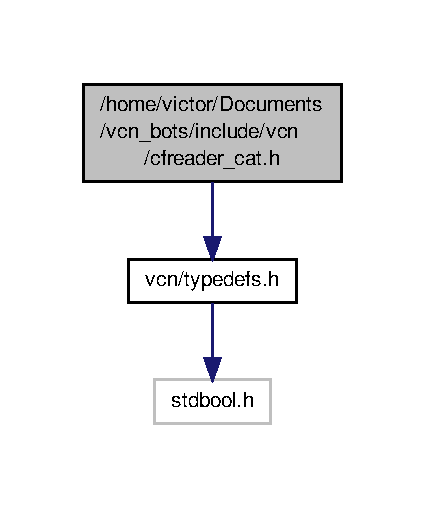
\includegraphics[width=204pt]{cfreader__cat_8h__incl}
\end{center}
\end{figure}
\subsection*{Typedefs}
\begin{DoxyCompactItemize}
\item 
\hypertarget{cfreader__cat_8h_a670e5720a4361f636ef92a258089e2bc}{typedef struct vcn\+\_\+cfreader\+\_\+s {\bfseries vcn\+\_\+cfreader\+\_\+t}}\label{cfreader__cat_8h_a670e5720a4361f636ef92a258089e2bc}

\end{DoxyCompactItemize}
\subsection*{Functions}
\begin{DoxyCompactItemize}
\item 
\hypertarget{cfreader__cat_8h_a410668e58054589cd04257768cf7e4a7}{vcn\+\_\+cfreader\+\_\+t $\ast$ {\bfseries vcn\+\_\+cfreader\+\_\+create} (const char $\ast$filename, const char $\ast$line\+\_\+comment\+\_\+token)}\label{cfreader__cat_8h_a410668e58054589cd04257768cf7e4a7}

\item 
\hypertarget{cfreader__cat_8h_a8c33208139e1ec06616f311ce3e2f104}{char {\bfseries vcn\+\_\+cfreader\+\_\+read\+\_\+int} (vcn\+\_\+cfreader\+\_\+t $\ast$cfreader, int $\ast$val)}\label{cfreader__cat_8h_a8c33208139e1ec06616f311ce3e2f104}

\item 
\hypertarget{cfreader__cat_8h_a2274ca06d08408fde228990e5b2de177}{char {\bfseries vcn\+\_\+cfreader\+\_\+read\+\_\+uint} (vcn\+\_\+cfreader\+\_\+t $\ast$cfreader, uint $\ast$val)}\label{cfreader__cat_8h_a2274ca06d08408fde228990e5b2de177}

\item 
\hypertarget{cfreader__cat_8h_a3542d4d17f46698bfd00fd218878a52f}{char {\bfseries vcn\+\_\+cfreader\+\_\+read\+\_\+float} (vcn\+\_\+cfreader\+\_\+t $\ast$cfreader, float $\ast$val)}\label{cfreader__cat_8h_a3542d4d17f46698bfd00fd218878a52f}

\item 
\hypertarget{cfreader__cat_8h_accf21a750cc4c7ba69cdc7be41e1119d}{char {\bfseries vcn\+\_\+cfreader\+\_\+read\+\_\+double} (vcn\+\_\+cfreader\+\_\+t $\ast$cfreader, double $\ast$val)}\label{cfreader__cat_8h_accf21a750cc4c7ba69cdc7be41e1119d}

\item 
\hypertarget{cfreader__cat_8h_ac69e16ca238851d1ffcbf1ba1f878586}{char {\bfseries vcn\+\_\+cfreader\+\_\+read\+\_\+bool} (vcn\+\_\+cfreader\+\_\+t $\ast$cfreader, bool $\ast$val)}\label{cfreader__cat_8h_ac69e16ca238851d1ffcbf1ba1f878586}

\item 
\hypertarget{cfreader__cat_8h_a990dbecbfdc83de4d66d4203809bb4d2}{char $\ast$ {\bfseries vcn\+\_\+cfreader\+\_\+read\+\_\+and\+\_\+allocate\+\_\+string} (vcn\+\_\+cfreader\+\_\+t $\ast$cfreader)}\label{cfreader__cat_8h_a990dbecbfdc83de4d66d4203809bb4d2}

\item 
\hypertarget{cfreader__cat_8h_adce71fba4f64c2ba09def17b7157c0d3}{void {\bfseries vcn\+\_\+cfreader\+\_\+destroy} (vcn\+\_\+cfreader\+\_\+t $\ast$cfreader)}\label{cfreader__cat_8h_adce71fba4f64c2ba09def17b7157c0d3}

\end{DoxyCompactItemize}


\subsection{Detailed Description}
Util to read customized file formats in plain text. 

\begin{DoxyAuthor}{Author}
Victor Eduardo Cardoso Nungaray ~\newline
 victorc@cimat.\+mx ~\newline
 \href{https://twitter.com/victore_cardoso}{\tt @victore\+\_\+cardoso } 
\end{DoxyAuthor}
\begin{DoxyDate}{Date}
14 August 2015
\end{DoxyDate}
\begin{DoxyParagraph}{License\+:}
This piece of code is in the P\+U\+B\+L\+I\+C D\+O\+M\+A\+I\+N, if your government does not recognizes such a dedication, then you are granted a perpetual and irrevocable license to copy and modify this file however you want. This does not imply any warranty. ~\newline
 Attributions and feedback are always welcome. 
\end{DoxyParagraph}

\hypertarget{dma__bot_8h}{\section{/home/victor/\+Documents/vcn\+\_\+bots/include/vcn/dma\+\_\+bot.h File Reference}
\label{dma__bot_8h}\index{/home/victor/\+Documents/vcn\+\_\+bots/include/vcn/dma\+\_\+bot.\+h@{/home/victor/\+Documents/vcn\+\_\+bots/include/vcn/dma\+\_\+bot.\+h}}
}


D\+M\+A File format designed to handle Dynamic Mesh Attributes.  


{\ttfamily \#include \char`\"{}vcn/typedefs.\+h\char`\"{}}\\*
Include dependency graph for dma\+\_\+bot.\+h\+:
\nopagebreak
\begin{figure}[H]
\begin{center}
\leavevmode
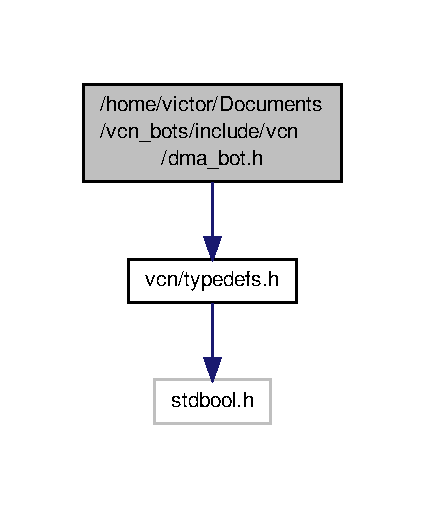
\includegraphics[width=204pt]{dma__bot_8h__incl}
\end{center}
\end{figure}
\subsection*{Typedefs}
\begin{DoxyCompactItemize}
\item 
\hypertarget{dma__bot_8h_aabf0c174943023de2b1d3d892008d4a1}{typedef struct vcn\+\_\+dma\+\_\+s {\bfseries vcn\+\_\+dma\+\_\+t}}\label{dma__bot_8h_aabf0c174943023de2b1d3d892008d4a1}

\end{DoxyCompactItemize}
\subsection*{Functions}
\begin{DoxyCompactItemize}
\item 
\hypertarget{dma__bot_8h_ad860f0a3755ad4a3309400f7bd1a91d2}{vcn\+\_\+dma\+\_\+t $\ast$ {\bfseries vcn\+\_\+dma\+\_\+create} (const char $\ast$filename)}\label{dma__bot_8h_ad860f0a3755ad4a3309400f7bd1a91d2}

\item 
\hypertarget{dma__bot_8h_ac9e8eff71352e4c12ca6c74fab430720}{void {\bfseries vcn\+\_\+dma\+\_\+destroy} (vcn\+\_\+dma\+\_\+t $\ast$dma)}\label{dma__bot_8h_ac9e8eff71352e4c12ca6c74fab430720}

\item 
\hypertarget{dma__bot_8h_aa5a4546a53854698fd3b605463a25474}{void {\bfseries vcn\+\_\+dma\+\_\+save} (vcn\+\_\+dma\+\_\+t $\ast$dma, const char $\ast$filename, bool save\+\_\+this\+\_\+time\+\_\+step(uint), bool save\+\_\+this\+\_\+attribute(uchar))}\label{dma__bot_8h_aa5a4546a53854698fd3b605463a25474}

\item 
\hypertarget{dma__bot_8h_a5371254cb4b0dacc7ca9eec891b3715c}{void {\bfseries vcn\+\_\+dma\+\_\+save\+\_\+as\+\_\+gid} (vcn\+\_\+dma\+\_\+t $\ast$dma, const char $\ast$filename\+\_\+msh, const char $\ast$filename\+\_\+res, bool save\+\_\+this\+\_\+time\+\_\+step(uint), bool save\+\_\+this\+\_\+attribute(uchar))}\label{dma__bot_8h_a5371254cb4b0dacc7ca9eec891b3715c}

\item 
\hypertarget{dma__bot_8h_a71699aacae6e4e7ca42865a614e17886}{bool {\bfseries vcn\+\_\+dma\+\_\+is\+\_\+2\+D} (vcn\+\_\+dma\+\_\+t $\ast$dma)}\label{dma__bot_8h_a71699aacae6e4e7ca42865a614e17886}

\item 
\hypertarget{dma__bot_8h_afff8b93835a6159dadaef25dfe4f179f}{bool {\bfseries vcn\+\_\+dma\+\_\+have\+\_\+simple\+\_\+precision} (vcn\+\_\+dma\+\_\+t $\ast$dma)}\label{dma__bot_8h_afff8b93835a6159dadaef25dfe4f179f}

\item 
\hypertarget{dma__bot_8h_ab5e2b47b73b52b745d865fb4547c04e6}{bool {\bfseries vcn\+\_\+dma\+\_\+have\+\_\+dynamic\+\_\+coordinates} (vcn\+\_\+dma\+\_\+t $\ast$dma)}\label{dma__bot_8h_ab5e2b47b73b52b745d865fb4547c04e6}

\item 
\hypertarget{dma__bot_8h_ad38e3fba5143f8cfa7332dc4b23b91bb}{bool {\bfseries vcn\+\_\+dma\+\_\+have\+\_\+variable\+\_\+step\+\_\+size} (vcn\+\_\+dma\+\_\+t $\ast$dma)}\label{dma__bot_8h_ad38e3fba5143f8cfa7332dc4b23b91bb}

\item 
\hypertarget{dma__bot_8h_a9faa7005ce12cbe1974490ff544afd53}{bool {\bfseries vcn\+\_\+dma\+\_\+have\+\_\+an\+\_\+attribute\+\_\+named} (vcn\+\_\+dma\+\_\+t $\ast$dma, const char $\ast$attribute\+\_\+name, uint $\ast$id\+\_\+out)}\label{dma__bot_8h_a9faa7005ce12cbe1974490ff544afd53}

\item 
\hypertarget{dma__bot_8h_a5f4a9d2adf259888cc328eae1ba2a765}{void $\ast$ {\bfseries vcn\+\_\+dma\+\_\+view\+\_\+static\+\_\+attribute} (vcn\+\_\+dma\+\_\+t $\ast$dma, uint id\+\_\+attr)}\label{dma__bot_8h_a5f4a9d2adf259888cc328eae1ba2a765}

\item 
\hypertarget{dma__bot_8h_a899fb7a8e21352ed1f1b87666adce036}{void $\ast$ {\bfseries vcn\+\_\+dma\+\_\+view\+\_\+dynamic\+\_\+attribute} (vcn\+\_\+dma\+\_\+t $\ast$dma, uint id\+\_\+attr, uint time\+\_\+step)}\label{dma__bot_8h_a899fb7a8e21352ed1f1b87666adce036}

\item 
\hypertarget{dma__bot_8h_a0d63a1ecf3a4d8cec3dd5f6a71d5e4f9}{void $\ast$ {\bfseries vcn\+\_\+dma\+\_\+view\+\_\+static\+\_\+attribute\+\_\+on\+\_\+vertices} (vcn\+\_\+dma\+\_\+t $\ast$dma, uint id\+\_\+attr)}\label{dma__bot_8h_a0d63a1ecf3a4d8cec3dd5f6a71d5e4f9}

\item 
\hypertarget{dma__bot_8h_a216f6699eb3ba58d9a4a8336103d224e}{void $\ast$ {\bfseries vcn\+\_\+dma\+\_\+view\+\_\+static\+\_\+attribute\+\_\+on\+\_\+elements} (vcn\+\_\+dma\+\_\+t $\ast$dma, uint id\+\_\+attr)}\label{dma__bot_8h_a216f6699eb3ba58d9a4a8336103d224e}

\item 
\hypertarget{dma__bot_8h_a9e8c1d6de3a7e0363a0b5d177d27abd0}{void $\ast$ {\bfseries vcn\+\_\+dma\+\_\+view\+\_\+dynamic\+\_\+attribute\+\_\+on\+\_\+vertices} (vcn\+\_\+dma\+\_\+t $\ast$dma, uint id\+\_\+attr, uint time\+\_\+step)}\label{dma__bot_8h_a9e8c1d6de3a7e0363a0b5d177d27abd0}

\item 
\hypertarget{dma__bot_8h_a3112a72cec5bfc9e1407124798bbdf7e}{void $\ast$ {\bfseries vcn\+\_\+dma\+\_\+view\+\_\+dynamic\+\_\+attribute\+\_\+on\+\_\+elements} (vcn\+\_\+dma\+\_\+t $\ast$dma, uint id\+\_\+attr, uint time\+\_\+step)}\label{dma__bot_8h_a3112a72cec5bfc9e1407124798bbdf7e}

\item 
\hypertarget{dma__bot_8h_ac63e595c0d9c306742c2026352084077}{void $\ast$$\ast$$\ast$ {\bfseries vcn\+\_\+dma\+\_\+view\+\_\+dynamic\+\_\+attributes\+\_\+of\+\_\+all\+\_\+time\+\_\+steps\+\_\+on\+\_\+vertices} (vcn\+\_\+dma\+\_\+t $\ast$dma)}\label{dma__bot_8h_ac63e595c0d9c306742c2026352084077}

\item 
\hypertarget{dma__bot_8h_a2bf5d99b1f679eef122b3c745f77c469}{void $\ast$$\ast$$\ast$ {\bfseries vcn\+\_\+dma\+\_\+view\+\_\+dynamic\+\_\+attributes\+\_\+of\+\_\+all\+\_\+time\+\_\+steps\+\_\+on\+\_\+elements} (vcn\+\_\+dma\+\_\+t $\ast$dma)}\label{dma__bot_8h_a2bf5d99b1f679eef122b3c745f77c469}

\item 
\hypertarget{dma__bot_8h_a1615748bf9f792c375d4af5d7fe9dcce}{void $\ast$ {\bfseries vcn\+\_\+dma\+\_\+view\+\_\+vertices} (vcn\+\_\+dma\+\_\+t $\ast$dma, uint time\+\_\+step)}\label{dma__bot_8h_a1615748bf9f792c375d4af5d7fe9dcce}

\item 
\hypertarget{dma__bot_8h_adfee6aa412c89751604abffd225b165a}{void $\ast$ {\bfseries vcn\+\_\+dma\+\_\+view\+\_\+delta\+\_\+time} (vcn\+\_\+dma\+\_\+t $\ast$dma)}\label{dma__bot_8h_adfee6aa412c89751604abffd225b165a}

\item 
\hypertarget{dma__bot_8h_a269297be53351437b02929b55d85c805}{uint {\bfseries vcn\+\_\+dma\+\_\+get\+\_\+\+N\+\_\+vertices} (vcn\+\_\+dma\+\_\+t $\ast$dma)}\label{dma__bot_8h_a269297be53351437b02929b55d85c805}

\item 
\hypertarget{dma__bot_8h_ab0caa0fa405cd7707cc84c3322dfc5b7}{uint {\bfseries vcn\+\_\+dma\+\_\+get\+\_\+\+N\+\_\+time\+\_\+steps} (vcn\+\_\+dma\+\_\+t $\ast$dma)}\label{dma__bot_8h_ab0caa0fa405cd7707cc84c3322dfc5b7}

\item 
\hypertarget{dma__bot_8h_af0267dd0209e8d2e2266a8ed56130f26}{uint {\bfseries vcn\+\_\+dma\+\_\+get\+\_\+dynamic\+\_\+chunk\+\_\+size} (vcn\+\_\+dma\+\_\+t $\ast$dma)}\label{dma__bot_8h_af0267dd0209e8d2e2266a8ed56130f26}

\item 
\hypertarget{dma__bot_8h_aa927b4d0ba0d915d3c962f6ddd19228c}{uint {\bfseries vcn\+\_\+dma\+\_\+get\+\_\+\+N\+\_\+attributes} (vcn\+\_\+dma\+\_\+t $\ast$dma)}\label{dma__bot_8h_aa927b4d0ba0d915d3c962f6ddd19228c}

\item 
\hypertarget{dma__bot_8h_ae80af8f229541955a14c2c231a4f4882}{uint {\bfseries vcn\+\_\+dma\+\_\+get\+\_\+\+N\+\_\+attributes\+\_\+on\+\_\+vertices} (vcn\+\_\+dma\+\_\+t $\ast$dma)}\label{dma__bot_8h_ae80af8f229541955a14c2c231a4f4882}

\item 
\hypertarget{dma__bot_8h_ad1b107400df3804db441b52ef314478d}{uint {\bfseries vcn\+\_\+dma\+\_\+get\+\_\+\+N\+\_\+attributes\+\_\+on\+\_\+elements} (vcn\+\_\+dma\+\_\+t $\ast$dma)}\label{dma__bot_8h_ad1b107400df3804db441b52ef314478d}

\item 
\hypertarget{dma__bot_8h_af4954ea7dd650ed9de32a0b24a800f0d}{uint {\bfseries vcn\+\_\+dma\+\_\+get\+\_\+\+N\+\_\+static\+\_\+attributes} (vcn\+\_\+dma\+\_\+t $\ast$dma)}\label{dma__bot_8h_af4954ea7dd650ed9de32a0b24a800f0d}

\item 
\hypertarget{dma__bot_8h_a1cfa46baa7655ae1a53524186ded31f7}{uint {\bfseries vcn\+\_\+dma\+\_\+get\+\_\+\+N\+\_\+dynamic\+\_\+attributes} (vcn\+\_\+dma\+\_\+t $\ast$dma)}\label{dma__bot_8h_a1cfa46baa7655ae1a53524186ded31f7}

\item 
\hypertarget{dma__bot_8h_a91fd39b9fdf87dd34a01eb0abd54fa96}{uint {\bfseries vcn\+\_\+dma\+\_\+get\+\_\+\+N\+\_\+static\+\_\+attributes\+\_\+on\+\_\+vertices} (vcn\+\_\+dma\+\_\+t $\ast$dma)}\label{dma__bot_8h_a91fd39b9fdf87dd34a01eb0abd54fa96}

\item 
\hypertarget{dma__bot_8h_ab045319b7a0fdd9581b0585944795836}{uint {\bfseries vcn\+\_\+dma\+\_\+get\+\_\+\+N\+\_\+static\+\_\+attributes\+\_\+on\+\_\+elements} (vcn\+\_\+dma\+\_\+t $\ast$dma)}\label{dma__bot_8h_ab045319b7a0fdd9581b0585944795836}

\item 
\hypertarget{dma__bot_8h_a84ad66177a050d49457890d791697f17}{uint {\bfseries vcn\+\_\+dma\+\_\+get\+\_\+\+N\+\_\+dynamic\+\_\+attributes\+\_\+on\+\_\+vertices} (vcn\+\_\+dma\+\_\+t $\ast$dma)}\label{dma__bot_8h_a84ad66177a050d49457890d791697f17}

\item 
\hypertarget{dma__bot_8h_aaf1d6cef0d37aaf684605f866a60e218}{uint {\bfseries vcn\+\_\+dma\+\_\+get\+\_\+\+N\+\_\+dynamic\+\_\+attributes\+\_\+on\+\_\+elements} (vcn\+\_\+dma\+\_\+t $\ast$dma)}\label{dma__bot_8h_aaf1d6cef0d37aaf684605f866a60e218}

\item 
\hypertarget{dma__bot_8h_a4d199268481c42fd10426785b44bf995}{uint {\bfseries vcn\+\_\+dma\+\_\+get\+\_\+\+N\+\_\+static\+\_\+class\+\_\+attributes\+\_\+on\+\_\+vertices} (vcn\+\_\+dma\+\_\+t $\ast$dma)}\label{dma__bot_8h_a4d199268481c42fd10426785b44bf995}

\item 
\hypertarget{dma__bot_8h_a767eaf2a93fd1ab9d250243979d246e4}{uint {\bfseries vcn\+\_\+dma\+\_\+get\+\_\+\+N\+\_\+static\+\_\+scalar\+\_\+attributes\+\_\+on\+\_\+vertices} (vcn\+\_\+dma\+\_\+t $\ast$dma)}\label{dma__bot_8h_a767eaf2a93fd1ab9d250243979d246e4}

\item 
\hypertarget{dma__bot_8h_a07f56b3cdad0c7b29a4f3813bb0f682a}{uint {\bfseries vcn\+\_\+dma\+\_\+get\+\_\+\+N\+\_\+static\+\_\+vector\+\_\+attributes\+\_\+on\+\_\+vertices} (vcn\+\_\+dma\+\_\+t $\ast$dma)}\label{dma__bot_8h_a07f56b3cdad0c7b29a4f3813bb0f682a}

\item 
\hypertarget{dma__bot_8h_ad8d590c1b8f4d8a11b6eac4f2d8865c4}{uint {\bfseries vcn\+\_\+dma\+\_\+get\+\_\+\+N\+\_\+static\+\_\+class\+\_\+attributes\+\_\+on\+\_\+elements} (vcn\+\_\+dma\+\_\+t $\ast$dma)}\label{dma__bot_8h_ad8d590c1b8f4d8a11b6eac4f2d8865c4}

\item 
\hypertarget{dma__bot_8h_a51f2c712e7f201feacd4c818244ef6fd}{uint {\bfseries vcn\+\_\+dma\+\_\+get\+\_\+\+N\+\_\+static\+\_\+scalar\+\_\+attributes\+\_\+on\+\_\+elements} (vcn\+\_\+dma\+\_\+t $\ast$dma)}\label{dma__bot_8h_a51f2c712e7f201feacd4c818244ef6fd}

\item 
\hypertarget{dma__bot_8h_aaa651201bbe47da33a000dd61b4133b9}{uint {\bfseries vcn\+\_\+dma\+\_\+get\+\_\+\+N\+\_\+static\+\_\+vector\+\_\+attributes\+\_\+on\+\_\+elements} (vcn\+\_\+dma\+\_\+t $\ast$dma)}\label{dma__bot_8h_aaa651201bbe47da33a000dd61b4133b9}

\item 
\hypertarget{dma__bot_8h_acb6fe9e54456a317c274ed0a8e2d65fc}{uint {\bfseries vcn\+\_\+dma\+\_\+get\+\_\+\+N\+\_\+dynamic\+\_\+class\+\_\+attributes\+\_\+on\+\_\+vertices} (vcn\+\_\+dma\+\_\+t $\ast$dma)}\label{dma__bot_8h_acb6fe9e54456a317c274ed0a8e2d65fc}

\item 
\hypertarget{dma__bot_8h_adbf319f813f858676eb383fd303f6007}{uint {\bfseries vcn\+\_\+dma\+\_\+get\+\_\+\+N\+\_\+dynamic\+\_\+scalar\+\_\+attributes\+\_\+on\+\_\+vertices} (vcn\+\_\+dma\+\_\+t $\ast$dma)}\label{dma__bot_8h_adbf319f813f858676eb383fd303f6007}

\item 
\hypertarget{dma__bot_8h_a7b7f5b4fb0cfa45c6e7eda056a21fe53}{uint {\bfseries vcn\+\_\+dma\+\_\+get\+\_\+\+N\+\_\+dynamic\+\_\+vector\+\_\+attributes\+\_\+on\+\_\+vertices} (vcn\+\_\+dma\+\_\+t $\ast$dma)}\label{dma__bot_8h_a7b7f5b4fb0cfa45c6e7eda056a21fe53}

\item 
\hypertarget{dma__bot_8h_a06797c9f5a6ab108e2ab4ad73e3a2a34}{uint {\bfseries vcn\+\_\+dma\+\_\+get\+\_\+\+N\+\_\+dynamic\+\_\+class\+\_\+attributes\+\_\+on\+\_\+elements} (vcn\+\_\+dma\+\_\+t $\ast$dma)}\label{dma__bot_8h_a06797c9f5a6ab108e2ab4ad73e3a2a34}

\item 
\hypertarget{dma__bot_8h_a0dea1c4c58392152ffaabb4c898474f6}{uint {\bfseries vcn\+\_\+dma\+\_\+get\+\_\+\+N\+\_\+dynamic\+\_\+scalar\+\_\+attributes\+\_\+on\+\_\+elements} (vcn\+\_\+dma\+\_\+t $\ast$dma)}\label{dma__bot_8h_a0dea1c4c58392152ffaabb4c898474f6}

\item 
\hypertarget{dma__bot_8h_a84b36aa1c06c520a1430de6fa935b3ee}{uint {\bfseries vcn\+\_\+dma\+\_\+get\+\_\+\+N\+\_\+dynamic\+\_\+vector\+\_\+attributes\+\_\+on\+\_\+elements} (vcn\+\_\+dma\+\_\+t $\ast$dma)}\label{dma__bot_8h_a84b36aa1c06c520a1430de6fa935b3ee}

\item 
\hypertarget{dma__bot_8h_a1ae1063b834d32ab5fff74dc581c612d}{char $\ast$ {\bfseries vcn\+\_\+dma\+\_\+view\+\_\+project\+\_\+name} (vcn\+\_\+dma\+\_\+t $\ast$dma)}\label{dma__bot_8h_a1ae1063b834d32ab5fff74dc581c612d}

\item 
\hypertarget{dma__bot_8h_a34b2f0517df78ff9f5734a1a09480df4}{char $\ast$ {\bfseries vcn\+\_\+dma\+\_\+view\+\_\+author\+\_\+name} (vcn\+\_\+dma\+\_\+t $\ast$dma)}\label{dma__bot_8h_a34b2f0517df78ff9f5734a1a09480df4}

\item 
\hypertarget{dma__bot_8h_a657e2ca421dd4b7f82f9ff64f3cff577}{char $\ast$ {\bfseries vcn\+\_\+dma\+\_\+allocate\+\_\+and\+\_\+get\+\_\+project\+\_\+name} (vcn\+\_\+dma\+\_\+t $\ast$dma)}\label{dma__bot_8h_a657e2ca421dd4b7f82f9ff64f3cff577}

\item 
\hypertarget{dma__bot_8h_a2fe6d6f8e2bc5b60825c56d936275e2d}{char $\ast$ {\bfseries vcn\+\_\+dma\+\_\+allocate\+\_\+and\+\_\+get\+\_\+author\+\_\+name} (vcn\+\_\+dma\+\_\+t $\ast$dma)}\label{dma__bot_8h_a2fe6d6f8e2bc5b60825c56d936275e2d}

\item 
\hypertarget{dma__bot_8h_a449881d8d624ed1e4d0208add9566a93}{char $\ast$ {\bfseries vcn\+\_\+dma\+\_\+view\+\_\+ith\+\_\+attribute\+\_\+name} (vcn\+\_\+dma\+\_\+t $\ast$dma, uint i)}\label{dma__bot_8h_a449881d8d624ed1e4d0208add9566a93}

\item 
\hypertarget{dma__bot_8h_accd472a5711712e224390312ad6677d2}{char $\ast$ {\bfseries vcn\+\_\+dma\+\_\+allocate\+\_\+and\+\_\+get\+\_\+ith\+\_\+attribute\+\_\+name} (vcn\+\_\+dma\+\_\+t $\ast$dma, uint i)}\label{dma__bot_8h_accd472a5711712e224390312ad6677d2}

\item 
\hypertarget{dma__bot_8h_ae063a3fec49aa0050bdca79d5f72742e}{char {\bfseries vcn\+\_\+dma\+\_\+get\+\_\+ith\+\_\+attribute\+\_\+type} (vcn\+\_\+dma\+\_\+t $\ast$dma, uint i)}\label{dma__bot_8h_ae063a3fec49aa0050bdca79d5f72742e}

\item 
\hypertarget{dma__bot_8h_a1c1e22bd972f10ad1c224ee57554d40f}{uchar {\bfseries vcn\+\_\+dma\+\_\+get\+\_\+ith\+\_\+attribute\+\_\+\+N\+\_\+components} (vcn\+\_\+dma\+\_\+t $\ast$dma, uint i)}\label{dma__bot_8h_a1c1e22bd972f10ad1c224ee57554d40f}

\item 
\hypertarget{dma__bot_8h_a431ad6c66d568b893bfd67e8dfa36d5e}{bool {\bfseries vcn\+\_\+dma\+\_\+is\+\_\+ith\+\_\+attribute\+\_\+upon\+\_\+vertices} (vcn\+\_\+dma\+\_\+t $\ast$dma, uint i)}\label{dma__bot_8h_a431ad6c66d568b893bfd67e8dfa36d5e}

\item 
\hypertarget{dma__bot_8h_a73203ca806fe50013a74045b7f02ccd1}{bool {\bfseries vcn\+\_\+dma\+\_\+is\+\_\+ith\+\_\+attribute\+\_\+upon\+\_\+elements} (vcn\+\_\+dma\+\_\+t $\ast$dma, uint i)}\label{dma__bot_8h_a73203ca806fe50013a74045b7f02ccd1}

\item 
\hypertarget{dma__bot_8h_aec602aa25668ef65211a8126b5fbb754}{bool {\bfseries vcn\+\_\+dma\+\_\+is\+\_\+ith\+\_\+attribute\+\_\+static} (vcn\+\_\+dma\+\_\+t $\ast$dma, uint i)}\label{dma__bot_8h_aec602aa25668ef65211a8126b5fbb754}

\item 
\hypertarget{dma__bot_8h_a8237de7108f89962ef5231106be7f071}{bool {\bfseries vcn\+\_\+dma\+\_\+is\+\_\+ith\+\_\+attribute\+\_\+dynamic} (vcn\+\_\+dma\+\_\+t $\ast$dma, uint i)}\label{dma__bot_8h_a8237de7108f89962ef5231106be7f071}

\item 
\hypertarget{dma__bot_8h_ad6a7cf32bc238a13cec33d515d84e65c}{bool {\bfseries vcn\+\_\+dma\+\_\+is\+\_\+ith\+\_\+attribute\+\_\+a\+\_\+class\+\_\+type} (vcn\+\_\+dma\+\_\+t $\ast$dma, uint i)}\label{dma__bot_8h_ad6a7cf32bc238a13cec33d515d84e65c}

\item 
\hypertarget{dma__bot_8h_a90f7065cef1fce05706c8c2615c64fb0}{bool {\bfseries vcn\+\_\+dma\+\_\+is\+\_\+ith\+\_\+attribute\+\_\+a\+\_\+scalar\+\_\+type} (vcn\+\_\+dma\+\_\+t $\ast$dma, uint i)}\label{dma__bot_8h_a90f7065cef1fce05706c8c2615c64fb0}

\item 
\hypertarget{dma__bot_8h_a75459ec28f1ac327be35c9995e565f11}{bool {\bfseries vcn\+\_\+dma\+\_\+is\+\_\+ith\+\_\+attribute\+\_\+a\+\_\+vector\+\_\+type} (vcn\+\_\+dma\+\_\+t $\ast$dma, uint i)}\label{dma__bot_8h_a75459ec28f1ac327be35c9995e565f11}

\item 
\hypertarget{dma__bot_8h_a048e039791d6f8a05dda134a65e34226}{uint {\bfseries vcn\+\_\+dma\+\_\+get\+\_\+\+N\+\_\+elements} (vcn\+\_\+dma\+\_\+t $\ast$dma)}\label{dma__bot_8h_a048e039791d6f8a05dda134a65e34226}

\item 
\hypertarget{dma__bot_8h_a7bdcc11b20f78ffcb9e9d46583a7411c}{uint {\bfseries vcn\+\_\+dma\+\_\+get\+\_\+\+N\+\_\+trg\+\_\+elements} (vcn\+\_\+dma\+\_\+t $\ast$dma)}\label{dma__bot_8h_a7bdcc11b20f78ffcb9e9d46583a7411c}

\item 
\hypertarget{dma__bot_8h_ac07d70a2a6ccc22f8063fef75448a2da}{uint {\bfseries vcn\+\_\+dma\+\_\+get\+\_\+\+N\+\_\+cdr\+\_\+elements} (vcn\+\_\+dma\+\_\+t $\ast$dma)}\label{dma__bot_8h_ac07d70a2a6ccc22f8063fef75448a2da}

\item 
\hypertarget{dma__bot_8h_a19e8fa085a5ca64cbc5eeb3e2400030c}{int32\+\_\+t $\ast$ {\bfseries vcn\+\_\+dma\+\_\+view\+\_\+trg\+\_\+elem\+\_\+connectivity\+\_\+matrix} (vcn\+\_\+dma\+\_\+t $\ast$dma)}\label{dma__bot_8h_a19e8fa085a5ca64cbc5eeb3e2400030c}

\item 
\hypertarget{dma__bot_8h_aba0c8f1f04dd9ad953ff67ca34183d18}{uint {\bfseries vcn\+\_\+dma\+\_\+get\+\_\+\+N\+\_\+segments} (vcn\+\_\+dma\+\_\+t $\ast$dma)}\label{dma__bot_8h_aba0c8f1f04dd9ad953ff67ca34183d18}

\item 
\hypertarget{dma__bot_8h_ab31fe186a373dc4f336df0952bc29c65}{uint $\ast$ {\bfseries vcn\+\_\+dma\+\_\+view\+\_\+segments} (vcn\+\_\+dma\+\_\+t $\ast$dma)}\label{dma__bot_8h_ab31fe186a373dc4f336df0952bc29c65}

\item 
\hypertarget{dma__bot_8h_adbd70c48634925c0294fba7b6d31dd24}{uint {\bfseries vcn\+\_\+dma\+\_\+get\+\_\+global\+\_\+\+I\+D\+\_\+from\+\_\+local\+\_\+\+I\+D\+\_\+of\+\_\+attributes\+\_\+on\+\_\+vertices} (vcn\+\_\+dma\+\_\+t $\ast$dma, uint idx)}\label{dma__bot_8h_adbd70c48634925c0294fba7b6d31dd24}

\item 
\hypertarget{dma__bot_8h_a286a756eacb79c0b75a47867ad50ecac}{uint {\bfseries vcn\+\_\+dma\+\_\+get\+\_\+global\+\_\+\+I\+D\+\_\+from\+\_\+local\+\_\+\+I\+D\+\_\+of\+\_\+attributes\+\_\+on\+\_\+elements} (vcn\+\_\+dma\+\_\+t $\ast$dma, uint idx)}\label{dma__bot_8h_a286a756eacb79c0b75a47867ad50ecac}

\item 
\hypertarget{dma__bot_8h_ae0c302830d6219d279f550ef3e3c0957}{uint {\bfseries vcn\+\_\+dma\+\_\+get\+\_\+global\+\_\+\+I\+D\+\_\+from\+\_\+local\+\_\+\+I\+D\+\_\+of\+\_\+static\+\_\+attributes} (vcn\+\_\+dma\+\_\+t $\ast$dma, uint idx)}\label{dma__bot_8h_ae0c302830d6219d279f550ef3e3c0957}

\item 
\hypertarget{dma__bot_8h_abc7af84c16cc5a5961de81b6f20d6488}{uint {\bfseries vcn\+\_\+dma\+\_\+get\+\_\+global\+\_\+\+I\+D\+\_\+from\+\_\+local\+\_\+\+I\+D\+\_\+of\+\_\+dynamic\+\_\+attributes} (vcn\+\_\+dma\+\_\+t $\ast$dma, uint idx)}\label{dma__bot_8h_abc7af84c16cc5a5961de81b6f20d6488}

\item 
\hypertarget{dma__bot_8h_a241b5793b7512f73bca6b7493e84fbb1}{uint {\bfseries vcn\+\_\+dma\+\_\+get\+\_\+global\+\_\+\+I\+D\+\_\+from\+\_\+local\+\_\+\+I\+D\+\_\+of\+\_\+static\+\_\+attributes\+\_\+on\+\_\+vertices} (vcn\+\_\+dma\+\_\+t $\ast$dma, uint idx)}\label{dma__bot_8h_a241b5793b7512f73bca6b7493e84fbb1}

\item 
\hypertarget{dma__bot_8h_a7f035c24c2d476735f888a1b533e1d10}{uint {\bfseries vcn\+\_\+dma\+\_\+get\+\_\+global\+\_\+\+I\+D\+\_\+from\+\_\+local\+\_\+\+I\+D\+\_\+of\+\_\+static\+\_\+attributes\+\_\+on\+\_\+elements} (vcn\+\_\+dma\+\_\+t $\ast$dma, uint idx)}\label{dma__bot_8h_a7f035c24c2d476735f888a1b533e1d10}

\item 
\hypertarget{dma__bot_8h_add2531ee4cfd868563c21f8aca3054ee}{uint {\bfseries vcn\+\_\+dma\+\_\+get\+\_\+global\+\_\+\+I\+D\+\_\+from\+\_\+local\+\_\+\+I\+D\+\_\+of\+\_\+dynamic\+\_\+attributes\+\_\+on\+\_\+vertices} (vcn\+\_\+dma\+\_\+t $\ast$dma, uint idx)}\label{dma__bot_8h_add2531ee4cfd868563c21f8aca3054ee}

\item 
\hypertarget{dma__bot_8h_a6a6047dfcf24a0476827f64449849bab}{uint {\bfseries vcn\+\_\+dma\+\_\+get\+\_\+global\+\_\+\+I\+D\+\_\+from\+\_\+local\+\_\+\+I\+D\+\_\+of\+\_\+dynamic\+\_\+attributes\+\_\+on\+\_\+elements} (vcn\+\_\+dma\+\_\+t $\ast$dma, uint idx)}\label{dma__bot_8h_a6a6047dfcf24a0476827f64449849bab}

\item 
\hypertarget{dma__bot_8h_af046db11fecf43880bcfa9eade9588ae}{uint {\bfseries vcn\+\_\+dma\+\_\+get\+\_\+global\+\_\+\+I\+D\+\_\+from\+\_\+local\+\_\+\+I\+D\+\_\+of\+\_\+static\+\_\+class\+\_\+attributes\+\_\+on\+\_\+vertices} (vcn\+\_\+dma\+\_\+t $\ast$dma, uint idx)}\label{dma__bot_8h_af046db11fecf43880bcfa9eade9588ae}

\item 
\hypertarget{dma__bot_8h_a0c6973c5a8c897d526acc3004d5e988d}{uint {\bfseries vcn\+\_\+dma\+\_\+get\+\_\+global\+\_\+\+I\+D\+\_\+from\+\_\+local\+\_\+\+I\+D\+\_\+of\+\_\+static\+\_\+scalar\+\_\+attributes\+\_\+on\+\_\+vertices} (vcn\+\_\+dma\+\_\+t $\ast$dma, uint idx)}\label{dma__bot_8h_a0c6973c5a8c897d526acc3004d5e988d}

\item 
\hypertarget{dma__bot_8h_ad70f64c75ce30ad5e7b13fe38edf0b45}{uint {\bfseries vcn\+\_\+dma\+\_\+get\+\_\+global\+\_\+\+I\+D\+\_\+from\+\_\+local\+\_\+\+I\+D\+\_\+of\+\_\+static\+\_\+vector\+\_\+attributes\+\_\+on\+\_\+vertices} (vcn\+\_\+dma\+\_\+t $\ast$dma, uint idx)}\label{dma__bot_8h_ad70f64c75ce30ad5e7b13fe38edf0b45}

\item 
\hypertarget{dma__bot_8h_a605afa1a7aae9a80f6a638677103fc43}{uint {\bfseries vcn\+\_\+dma\+\_\+get\+\_\+global\+\_\+\+I\+D\+\_\+from\+\_\+local\+\_\+\+I\+D\+\_\+of\+\_\+static\+\_\+class\+\_\+attributes\+\_\+on\+\_\+elements} (vcn\+\_\+dma\+\_\+t $\ast$dma, uint idx)}\label{dma__bot_8h_a605afa1a7aae9a80f6a638677103fc43}

\item 
\hypertarget{dma__bot_8h_ab4bc51a8224fa357a6898362d1671031}{uint {\bfseries vcn\+\_\+dma\+\_\+get\+\_\+global\+\_\+\+I\+D\+\_\+from\+\_\+local\+\_\+\+I\+D\+\_\+of\+\_\+static\+\_\+scalar\+\_\+attributes\+\_\+on\+\_\+elements} (vcn\+\_\+dma\+\_\+t $\ast$dma, uint idx)}\label{dma__bot_8h_ab4bc51a8224fa357a6898362d1671031}

\item 
\hypertarget{dma__bot_8h_aa6c1d85d7a22123df5d1ebfb97500497}{uint {\bfseries vcn\+\_\+dma\+\_\+get\+\_\+global\+\_\+\+I\+D\+\_\+from\+\_\+local\+\_\+\+I\+D\+\_\+of\+\_\+static\+\_\+vector\+\_\+attributes\+\_\+on\+\_\+elements} (vcn\+\_\+dma\+\_\+t $\ast$dma, uint idx)}\label{dma__bot_8h_aa6c1d85d7a22123df5d1ebfb97500497}

\item 
\hypertarget{dma__bot_8h_a67942808fc205aabf91c2d03ebb5aea2}{uint {\bfseries vcn\+\_\+dma\+\_\+get\+\_\+global\+\_\+\+I\+D\+\_\+from\+\_\+local\+\_\+\+I\+D\+\_\+of\+\_\+dynamic\+\_\+class\+\_\+attributes\+\_\+on\+\_\+vertices} (vcn\+\_\+dma\+\_\+t $\ast$dma, uint idx)}\label{dma__bot_8h_a67942808fc205aabf91c2d03ebb5aea2}

\item 
\hypertarget{dma__bot_8h_a8d6eddaeef7d273d060d075abd280ada}{uint {\bfseries vcn\+\_\+dma\+\_\+get\+\_\+global\+\_\+\+I\+D\+\_\+from\+\_\+local\+\_\+\+I\+D\+\_\+of\+\_\+dynamic\+\_\+scalar\+\_\+attributes\+\_\+on\+\_\+vertices} (vcn\+\_\+dma\+\_\+t $\ast$dma, uint idx)}\label{dma__bot_8h_a8d6eddaeef7d273d060d075abd280ada}

\item 
\hypertarget{dma__bot_8h_ac649abdd821965bf5c435534057085cf}{uint {\bfseries vcn\+\_\+dma\+\_\+get\+\_\+global\+\_\+\+I\+D\+\_\+from\+\_\+local\+\_\+\+I\+D\+\_\+of\+\_\+dynamic\+\_\+vector\+\_\+attributes\+\_\+on\+\_\+vertices} (vcn\+\_\+dma\+\_\+t $\ast$dma, uint idx)}\label{dma__bot_8h_ac649abdd821965bf5c435534057085cf}

\item 
\hypertarget{dma__bot_8h_af05995641ad354e62f764267a68b1526}{uint {\bfseries vcn\+\_\+dma\+\_\+get\+\_\+global\+\_\+\+I\+D\+\_\+from\+\_\+local\+\_\+\+I\+D\+\_\+of\+\_\+dynamic\+\_\+class\+\_\+attributes\+\_\+on\+\_\+elements} (vcn\+\_\+dma\+\_\+t $\ast$dma, uint idx)}\label{dma__bot_8h_af05995641ad354e62f764267a68b1526}

\item 
\hypertarget{dma__bot_8h_a438fc0c0f9e53ed7663a7d62e9bed6b6}{uint {\bfseries vcn\+\_\+dma\+\_\+get\+\_\+global\+\_\+\+I\+D\+\_\+from\+\_\+local\+\_\+\+I\+D\+\_\+of\+\_\+dynamic\+\_\+scalar\+\_\+attributes\+\_\+on\+\_\+elements} (vcn\+\_\+dma\+\_\+t $\ast$dma, uint idx)}\label{dma__bot_8h_a438fc0c0f9e53ed7663a7d62e9bed6b6}

\item 
\hypertarget{dma__bot_8h_a73618cd5caf8f02f32b77103edbbbeda}{uint {\bfseries vcn\+\_\+dma\+\_\+get\+\_\+global\+\_\+\+I\+D\+\_\+from\+\_\+local\+\_\+\+I\+D\+\_\+of\+\_\+dynamic\+\_\+vector\+\_\+attributes\+\_\+on\+\_\+elements} (vcn\+\_\+dma\+\_\+t $\ast$dma, uint idx)}\label{dma__bot_8h_a73618cd5caf8f02f32b77103edbbbeda}

\item 
\hypertarget{dma__bot_8h_a2ac5311bd6f8f6f5fbe9f91bddcf6f9d}{float {\bfseries get\+\_\+value\+\_\+from\+\_\+array} (void $\ast$array1, void $\ast$array2, float alpha1, uchar sizeof\+\_\+real, char value\+\_\+type, uchar nth\+\_\+component, uchar vector\+\_\+length, uint i)}\label{dma__bot_8h_a2ac5311bd6f8f6f5fbe9f91bddcf6f9d}

\end{DoxyCompactItemize}


\subsection{Detailed Description}
D\+M\+A File format designed to handle Dynamic Mesh Attributes. 

\begin{DoxyAuthor}{Author}
Victor Eduardo Cardoso Nungaray ~\newline
 victorc@cimat.\+mx ~\newline
 \href{https://twitter.com/victore_cardoso}{\tt @victore\+\_\+cardoso } 
\end{DoxyAuthor}
\begin{DoxyDate}{Date}
14 August 2015
\end{DoxyDate}
\begin{DoxyParagraph}{License\+:}
This piece of code is in the P\+U\+B\+L\+I\+C D\+O\+M\+A\+I\+N, if your government does not recognizes such a dedication, then you are granted a perpetual and irrevocable license to copy and modify this file however you want. This does not imply any warranty. ~\newline
 Attributions and feedback are always welcome. 
\end{DoxyParagraph}

\hypertarget{fem__bot-coming__soon_8h}{\section{/home/victor/\+Documents/vcn\+\_\+bots/include/vcn/fem\+\_\+bot-\/coming\+\_\+soon.h File Reference}
\label{fem__bot-coming__soon_8h}\index{/home/victor/\+Documents/vcn\+\_\+bots/include/vcn/fem\+\_\+bot-\/coming\+\_\+soon.\+h@{/home/victor/\+Documents/vcn\+\_\+bots/include/vcn/fem\+\_\+bot-\/coming\+\_\+soon.\+h}}
}


Next features add to the Finite Element Bot.  


\subsection*{Functions}
\begin{DoxyCompactItemize}
\item 
\hypertarget{fem__bot-coming__soon_8h_a68db92ac75c7596f6063b0555a6172f0}{void {\bfseries vcn\+\_\+fem\+\_\+enrich\+\_\+output} (const char $\ast$vcn\+\_\+dma\+\_\+filename, const char $\ast$vcn\+\_\+dma\+\_\+filename\+\_\+enhanced, const vcn\+\_\+fem\+\_\+elem\+\_\+t $\ast$const elemtype, const vcn\+\_\+fem\+\_\+material\+\_\+t $\ast$const material, bool add\+\_\+main\+\_\+strain, bool add\+\_\+real\+\_\+stress, bool add\+\_\+main\+\_\+stress, bool add\+\_\+effective\+\_\+stress, bool add\+\_\+main\+\_\+effective\+\_\+stress, bool add\+\_\+von\+\_\+mises\+\_\+stress, bool add\+\_\+error\+\_\+based\+\_\+on\+\_\+strain)}\label{fem__bot-coming__soon_8h_a68db92ac75c7596f6063b0555a6172f0}

\item 
\hypertarget{fem__bot-coming__soon_8h_a3a7e0c05255014a232059a75cd89e336}{void {\bfseries vcn\+\_\+fem\+\_\+analyze\+\_\+reaction} (const char $\ast$vcn\+\_\+dma\+\_\+filename, const char $\ast$data\+\_\+filename, bool track\+\_\+vertical\+\_\+reaction, bool track\+\_\+horizontal\+\_\+reaction, bool track\+\_\+reaction\+\_\+magnitude, uint N\+\_\+nodes, uint $\ast$nodes)}\label{fem__bot-coming__soon_8h_a3a7e0c05255014a232059a75cd89e336}

\end{DoxyCompactItemize}


\subsection{Detailed Description}
Next features add to the Finite Element Bot. 

\begin{DoxyAuthor}{Author}
Victor Eduardo Cardoso Nungaray ~\newline
 victorc@cimat.\+mx ~\newline
 \href{https://twitter.com/victore_cardoso}{\tt @victore\+\_\+cardoso } 
\end{DoxyAuthor}
\begin{DoxyDate}{Date}
10 August 2015
\end{DoxyDate}
\begin{DoxyParagraph}{License\+:}
This piece of code is in the P\+U\+B\+L\+I\+C D\+O\+M\+A\+I\+N, if your government does not recognizes such a dedication, then you are granted a perpetual and irrevocable license to copy and modify this file however you want. This does not imply any warranty. ~\newline
 Attributions and feedback are always welcome. 
\end{DoxyParagraph}

\hypertarget{fem__bot_8h}{\section{/home/victor/\+Documents/vcn\+\_\+bots/include/vcn/fem\+\_\+bot.h File Reference}
\label{fem__bot_8h}\index{/home/victor/\+Documents/vcn\+\_\+bots/include/vcn/fem\+\_\+bot.\+h@{/home/victor/\+Documents/vcn\+\_\+bots/include/vcn/fem\+\_\+bot.\+h}}
}


F\+E\+M bot will assemble the linear systems of well stablished F\+E problems, such as solid mechanics and heat diffusion.  


{\ttfamily \#include \char`\"{}vcn/typedefs.\+h\char`\"{}}\\*
{\ttfamily \#include \char`\"{}vcn/geometric\+\_\+bot.\+h\char`\"{}}\\*
{\ttfamily \#include \char`\"{}vcn/sparse\+\_\+bot.\+h\char`\"{}}\\*
Include dependency graph for fem\+\_\+bot.\+h\+:
\nopagebreak
\begin{figure}[H]
\begin{center}
\leavevmode
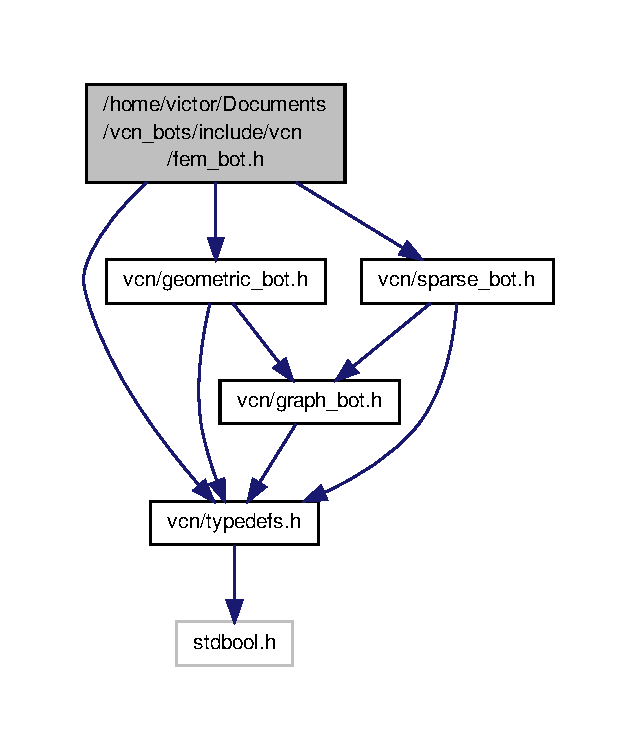
\includegraphics[width=306pt]{fem__bot_8h__incl}
\end{center}
\end{figure}
\subsection*{Classes}
\begin{DoxyCompactItemize}
\item 
struct \hyperlink{structvcn__bcond__t}{vcn\+\_\+bcond\+\_\+t}
\item 
struct \hyperlink{structvcn__fem__output__t}{vcn\+\_\+fem\+\_\+output\+\_\+t}
\end{DoxyCompactItemize}
\subsection*{Typedefs}
\begin{DoxyCompactItemize}
\item 
\hypertarget{fem__bot_8h_a1960f237d9a84c9671dc61072e6a3eb3}{typedef struct vcn\+\_\+fem\+\_\+elem\+\_\+s {\bfseries vcn\+\_\+fem\+\_\+elem\+\_\+t}}\label{fem__bot_8h_a1960f237d9a84c9671dc61072e6a3eb3}

\item 
\hypertarget{fem__bot_8h_a15d726942269c6b42f99208bb2c96650}{typedef struct vcn\+\_\+fem\+\_\+material\+\_\+s {\bfseries vcn\+\_\+fem\+\_\+material\+\_\+t}}\label{fem__bot_8h_a15d726942269c6b42f99208bb2c96650}

\item 
\hypertarget{fem__bot_8h_a6f86d7a05fd636d977a565fa2deff097}{typedef struct vcn\+\_\+fem\+\_\+implicit\+\_\+s {\bfseries vcn\+\_\+fem\+\_\+implicit\+\_\+t}}\label{fem__bot_8h_a6f86d7a05fd636d977a565fa2deff097}

\end{DoxyCompactItemize}
\subsection*{Functions}
\begin{DoxyCompactItemize}
\item 
\hypertarget{fem__bot_8h_a6e0a209fa762e820ed5040b7f4c4694d}{vcn\+\_\+fem\+\_\+implicit\+\_\+t $\ast$ {\bfseries vcn\+\_\+fem\+\_\+implicit\+\_\+create} ()}\label{fem__bot_8h_a6e0a209fa762e820ed5040b7f4c4694d}

\item 
\hypertarget{fem__bot_8h_aab49d1d0631f87de940b208e43c3172c}{void {\bfseries vcn\+\_\+fem\+\_\+implicit\+\_\+destroy} (vcn\+\_\+fem\+\_\+implicit\+\_\+t $\ast$isparams)}\label{fem__bot_8h_aab49d1d0631f87de940b208e43c3172c}

\item 
\hypertarget{fem__bot_8h_a0821a5344b977d6dbede10f086424e20}{void {\bfseries vcn\+\_\+fem\+\_\+implicit\+\_\+set\+\_\+\+N\+\_\+steps} (vcn\+\_\+fem\+\_\+implicit\+\_\+t $\ast$isparams, uint N\+\_\+time\+\_\+steps)}\label{fem__bot_8h_a0821a5344b977d6dbede10f086424e20}

\item 
\hypertarget{fem__bot_8h_adf5e9f817d29012a79428aefc2f3772a}{void {\bfseries vcn\+\_\+fem\+\_\+implicit\+\_\+set\+\_\+\+N\+\_\+max\+\_\+iter} (vcn\+\_\+fem\+\_\+implicit\+\_\+t $\ast$isparams, uint N\+\_\+max\+\_\+iter)}\label{fem__bot_8h_adf5e9f817d29012a79428aefc2f3772a}

\item 
\hypertarget{fem__bot_8h_a0cc40abe6a12aa01cca7564a788dbd87}{void {\bfseries vcn\+\_\+fem\+\_\+implicit\+\_\+set\+\_\+\+N\+\_\+max\+\_\+iter\+\_\+without\+\_\+enhance} (vcn\+\_\+fem\+\_\+implicit\+\_\+t $\ast$isparams, uint N\+\_\+max\+\_\+iter)}\label{fem__bot_8h_a0cc40abe6a12aa01cca7564a788dbd87}

\item 
\hypertarget{fem__bot_8h_a3a7278bb6f47556297a3551166fc2757}{void {\bfseries vcn\+\_\+fem\+\_\+implicit\+\_\+set\+\_\+residual\+\_\+tolerance} (vcn\+\_\+fem\+\_\+implicit\+\_\+t $\ast$isparams, double penergy\+\_\+tol)}\label{fem__bot_8h_a3a7278bb6f47556297a3551166fc2757}

\item 
\hypertarget{fem__bot_8h_a96345d73fe8dc4465f9af450387a954f}{uint {\bfseries vcn\+\_\+fem\+\_\+implicit\+\_\+get\+\_\+\+N\+\_\+steps} (vcn\+\_\+fem\+\_\+implicit\+\_\+t $\ast$isparams)}\label{fem__bot_8h_a96345d73fe8dc4465f9af450387a954f}

\item 
\hypertarget{fem__bot_8h_afca7295a2df67d2a53353431ef166dca}{uint {\bfseries vcn\+\_\+fem\+\_\+implicit\+\_\+get\+\_\+\+N\+\_\+max\+\_\+iter} (vcn\+\_\+fem\+\_\+implicit\+\_\+t $\ast$isparams)}\label{fem__bot_8h_afca7295a2df67d2a53353431ef166dca}

\item 
\hypertarget{fem__bot_8h_a1ca209e0d22c6633f4ad8709053df409}{uint {\bfseries vcn\+\_\+fem\+\_\+implicit\+\_\+get\+\_\+\+N\+\_\+max\+\_\+iter\+\_\+without\+\_\+enhance} (vcn\+\_\+fem\+\_\+implicit\+\_\+t $\ast$isparams)}\label{fem__bot_8h_a1ca209e0d22c6633f4ad8709053df409}

\item 
\hypertarget{fem__bot_8h_aabefc64cf277cfd45f606b250dfa8d6d}{double {\bfseries vcn\+\_\+fem\+\_\+implicit\+\_\+get\+\_\+residual\+\_\+tolerance} (vcn\+\_\+fem\+\_\+implicit\+\_\+t $\ast$isparams)}\label{fem__bot_8h_aabefc64cf277cfd45f606b250dfa8d6d}

\item 
\hypertarget{fem__bot_8h_a9ed0df3a08d6631a1cde7d6932d9f93a}{vcn\+\_\+fem\+\_\+material\+\_\+t $\ast$ {\bfseries vcn\+\_\+fem\+\_\+material\+\_\+create} ()}\label{fem__bot_8h_a9ed0df3a08d6631a1cde7d6932d9f93a}

\item 
\hypertarget{fem__bot_8h_a03c5001e38c3bec8f4fd87a7c8bb1200}{void {\bfseries vcn\+\_\+fem\+\_\+material\+\_\+destroy} (vcn\+\_\+fem\+\_\+material\+\_\+t $\ast$mat)}\label{fem__bot_8h_a03c5001e38c3bec8f4fd87a7c8bb1200}

\item 
\hypertarget{fem__bot_8h_a253e4585ca16984bb84658c42fa64fa8}{void {\bfseries vcn\+\_\+fem\+\_\+material\+\_\+set\+\_\+poisson\+\_\+module} (vcn\+\_\+fem\+\_\+material\+\_\+t $\ast$mat, double pmodule)}\label{fem__bot_8h_a253e4585ca16984bb84658c42fa64fa8}

\item 
\hypertarget{fem__bot_8h_aaae0ab63d75e70b3abcbce3062cc6b05}{void {\bfseries vcn\+\_\+fem\+\_\+material\+\_\+set\+\_\+elasticity\+\_\+module} (vcn\+\_\+fem\+\_\+material\+\_\+t $\ast$mat, double emodule)}\label{fem__bot_8h_aaae0ab63d75e70b3abcbce3062cc6b05}

\item 
\hypertarget{fem__bot_8h_ae365aa1b369277bb3d1026d10eb7741f}{void {\bfseries vcn\+\_\+fem\+\_\+material\+\_\+set\+\_\+density} (vcn\+\_\+fem\+\_\+material\+\_\+t $\ast$mat, double density)}\label{fem__bot_8h_ae365aa1b369277bb3d1026d10eb7741f}

\item 
\hypertarget{fem__bot_8h_a9e274bd468a268eafdeb2a0a9a21a35b}{void {\bfseries vcn\+\_\+fem\+\_\+material\+\_\+set\+\_\+fracture\+\_\+energy} (vcn\+\_\+fem\+\_\+material\+\_\+t $\ast$mat, double frac\+\_\+energy)}\label{fem__bot_8h_a9e274bd468a268eafdeb2a0a9a21a35b}

\item 
\hypertarget{fem__bot_8h_a58064b76bf2845eb2b3c2063f9f13c1a}{void {\bfseries vcn\+\_\+fem\+\_\+material\+\_\+set\+\_\+traction\+\_\+limit\+\_\+stress} (vcn\+\_\+fem\+\_\+material\+\_\+t $\ast$mat, double max\+\_\+stress)}\label{fem__bot_8h_a58064b76bf2845eb2b3c2063f9f13c1a}

\item 
\hypertarget{fem__bot_8h_acaaebfa88c4f89b78f229c4a64a7af65}{void {\bfseries vcn\+\_\+fem\+\_\+material\+\_\+set\+\_\+compression\+\_\+limit\+\_\+stress} (vcn\+\_\+fem\+\_\+material\+\_\+t $\ast$mat, double max\+\_\+stress)}\label{fem__bot_8h_acaaebfa88c4f89b78f229c4a64a7af65}

\item 
\hypertarget{fem__bot_8h_a1d68d578a6f4bfd5d7adcbfd19ec271c}{double {\bfseries vcn\+\_\+fem\+\_\+material\+\_\+get\+\_\+poisson\+\_\+module} (const vcn\+\_\+fem\+\_\+material\+\_\+t $\ast$const mat)}\label{fem__bot_8h_a1d68d578a6f4bfd5d7adcbfd19ec271c}

\item 
\hypertarget{fem__bot_8h_ae09d11b0ecb173c2546f5401a58cd257}{double {\bfseries vcn\+\_\+fem\+\_\+material\+\_\+get\+\_\+elasticity\+\_\+module} (const vcn\+\_\+fem\+\_\+material\+\_\+t $\ast$const mat)}\label{fem__bot_8h_ae09d11b0ecb173c2546f5401a58cd257}

\item 
\hypertarget{fem__bot_8h_a9d3a3b029d994ea502eb56a4d214ae95}{double {\bfseries vcn\+\_\+fem\+\_\+material\+\_\+get\+\_\+density} (const vcn\+\_\+fem\+\_\+material\+\_\+t $\ast$const mat)}\label{fem__bot_8h_a9d3a3b029d994ea502eb56a4d214ae95}

\item 
\hypertarget{fem__bot_8h_a7ea871a26279e69833efe37459455aa0}{double {\bfseries vcn\+\_\+fem\+\_\+material\+\_\+get\+\_\+fracture\+\_\+energy} (const vcn\+\_\+fem\+\_\+material\+\_\+t $\ast$const mat)}\label{fem__bot_8h_a7ea871a26279e69833efe37459455aa0}

\item 
\hypertarget{fem__bot_8h_ae4764b8f7d1b4d172ba2e6201ce0f01d}{double {\bfseries vcn\+\_\+fem\+\_\+material\+\_\+get\+\_\+traction\+\_\+limit\+\_\+stress} (const vcn\+\_\+fem\+\_\+material\+\_\+t $\ast$const mat)}\label{fem__bot_8h_ae4764b8f7d1b4d172ba2e6201ce0f01d}

\item 
\hypertarget{fem__bot_8h_a8b9ef465f23b354527f8223cecb15d4c}{double {\bfseries vcn\+\_\+fem\+\_\+material\+\_\+get\+\_\+compression\+\_\+limit\+\_\+stress} (const vcn\+\_\+fem\+\_\+material\+\_\+t $\ast$const mat)}\label{fem__bot_8h_a8b9ef465f23b354527f8223cecb15d4c}

\item 
\hypertarget{fem__bot_8h_acfa873ce2e48e4a7d0d45c732e7e6ec2}{void $\ast$ {\bfseries vcn\+\_\+fem\+\_\+material\+\_\+get\+\_\+damage\+\_\+function} (const vcn\+\_\+fem\+\_\+material\+\_\+t $\ast$const mat)}\label{fem__bot_8h_acfa873ce2e48e4a7d0d45c732e7e6ec2}

\item 
\hypertarget{fem__bot_8h_afcd3b6a1c6a673684b4a9f03242591e8}{int {\bfseries vcn\+\_\+fem\+\_\+material\+\_\+verify} (vcn\+\_\+fem\+\_\+material\+\_\+t $\ast$material)}\label{fem__bot_8h_afcd3b6a1c6a673684b4a9f03242591e8}

\item 
\hypertarget{fem__bot_8h_a280c2ff2b440b94569511bd4c07dd3d4}{\hyperlink{structvcn__bcond__t}{vcn\+\_\+bcond\+\_\+t} $\ast$ {\bfseries vcn\+\_\+fem\+\_\+bcond\+\_\+create} ()}\label{fem__bot_8h_a280c2ff2b440b94569511bd4c07dd3d4}

\item 
\hypertarget{fem__bot_8h_a50da87b565fea1cf8d7102637475e650}{\hyperlink{structvcn__bcond__t}{vcn\+\_\+bcond\+\_\+t} $\ast$ {\bfseries vcn\+\_\+fem\+\_\+bcond\+\_\+clone} (const \hyperlink{structvcn__bcond__t}{vcn\+\_\+bcond\+\_\+t} $\ast$const bconditions)}\label{fem__bot_8h_a50da87b565fea1cf8d7102637475e650}

\item 
\hypertarget{fem__bot_8h_a5fc48cba1d23cf07b61b93cdb454eebf}{\hyperlink{structvcn__bcond__t}{vcn\+\_\+bcond\+\_\+t} $\ast$ {\bfseries vcn\+\_\+fem\+\_\+bcond\+\_\+read} (const char $\ast$filename)}\label{fem__bot_8h_a5fc48cba1d23cf07b61b93cdb454eebf}

\item 
\hypertarget{fem__bot_8h_aec3223c95098bfb01b0d57d5b05426d6}{void {\bfseries vcn\+\_\+fem\+\_\+bcond\+\_\+save} (const \hyperlink{structvcn__bcond__t}{vcn\+\_\+bcond\+\_\+t} $\ast$const bconditions, const char $\ast$filename)}\label{fem__bot_8h_aec3223c95098bfb01b0d57d5b05426d6}

\item 
\hypertarget{fem__bot_8h_aad1a0ff13d74dd4d479f872084a19ef9}{void {\bfseries vcn\+\_\+fem\+\_\+bcond\+\_\+copy} (\hyperlink{structvcn__bcond__t}{vcn\+\_\+bcond\+\_\+t} $\ast$cpy, const \hyperlink{structvcn__bcond__t}{vcn\+\_\+bcond\+\_\+t} $\ast$const src)}\label{fem__bot_8h_aad1a0ff13d74dd4d479f872084a19ef9}

\item 
\hypertarget{fem__bot_8h_acb398c500e611b24a5b4673da672abd8}{void {\bfseries vcn\+\_\+fem\+\_\+bcond\+\_\+clear} (\hyperlink{structvcn__bcond__t}{vcn\+\_\+bcond\+\_\+t} $\ast$bconditions)}\label{fem__bot_8h_acb398c500e611b24a5b4673da672abd8}

\item 
\hypertarget{fem__bot_8h_a93c02289e868fb33e769ea61ba2cac67}{void {\bfseries vcn\+\_\+fem\+\_\+bcond\+\_\+destroy} (\hyperlink{structvcn__bcond__t}{vcn\+\_\+bcond\+\_\+t} $\ast$bconditions)}\label{fem__bot_8h_a93c02289e868fb33e769ea61ba2cac67}

\item 
\hypertarget{fem__bot_8h_aa11741f7a461d4daf7e44f5d97e88c6c}{void {\bfseries vcn\+\_\+fem\+\_\+bcond\+\_\+printf} (const \hyperlink{structvcn__bcond__t}{vcn\+\_\+bcond\+\_\+t} $\ast$const bconditions)}\label{fem__bot_8h_aa11741f7a461d4daf7e44f5d97e88c6c}

\item 
\hypertarget{fem__bot_8h_afabd73ec672fd81ab6eb84fb59e34725}{\hyperlink{structvcn__bcond__t}{vcn\+\_\+bcond\+\_\+t} $\ast$ {\bfseries vcn\+\_\+fem\+\_\+bcond\+\_\+create\+\_\+from\+\_\+model\+\_\+to\+\_\+mesh} (const \hyperlink{geometric__bot_8h_af753a8fb5e30b4d81a02489e92b54df2}{vcn\+\_\+msh3trg\+\_\+t} $\ast$const msh3trg, const \hyperlink{structvcn__bcond__t}{vcn\+\_\+bcond\+\_\+t} $\ast$const bconditions)}\label{fem__bot_8h_afabd73ec672fd81ab6eb84fb59e34725}

\item 
\hypertarget{fem__bot_8h_ac20ef2ea5b8ae85c4f072006672707ac}{vcn\+\_\+fem\+\_\+elem\+\_\+t $\ast$ {\bfseries vcn\+\_\+fem\+\_\+elem\+\_\+create\+\_\+triangle} ()}\label{fem__bot_8h_ac20ef2ea5b8ae85c4f072006672707ac}

\item 
\hypertarget{fem__bot_8h_a2b72e7aa584bc187b053b4c3ffc7b932}{void {\bfseries vcn\+\_\+fem\+\_\+elem\+\_\+destroy} (vcn\+\_\+fem\+\_\+elem\+\_\+t $\ast$elemtype)}\label{fem__bot_8h_a2b72e7aa584bc187b053b4c3ffc7b932}

\item 
\hypertarget{fem__bot_8h_aa4e8da7af135432150ff0ff889e7ec21}{uint {\bfseries vcn\+\_\+fem\+\_\+elem\+\_\+get\+\_\+\+N\+\_\+nodes} (const vcn\+\_\+fem\+\_\+elem\+\_\+t $\ast$const elemtype)}\label{fem__bot_8h_aa4e8da7af135432150ff0ff889e7ec21}

\item 
\hypertarget{fem__bot_8h_a5c8622a52f929adda5629290811a2fc2}{void $\ast$ {\bfseries vcn\+\_\+fem\+\_\+elem\+\_\+get\+\_\+ith\+\_\+shape\+\_\+function} (const vcn\+\_\+fem\+\_\+elem\+\_\+t $\ast$const elemtype, uint i)}\label{fem__bot_8h_a5c8622a52f929adda5629290811a2fc2}

\item 
\hypertarget{fem__bot_8h_a6efe2ca5819425df832c8777a5e85153}{uint {\bfseries vcn\+\_\+fem\+\_\+elem\+\_\+get\+\_\+closest\+\_\+\+Gauss\+\_\+\+Point\+\_\+to\+\_\+the\+\_\+ith\+\_\+node} (const vcn\+\_\+fem\+\_\+elem\+\_\+t $\ast$const elemtype, uint i)}\label{fem__bot_8h_a6efe2ca5819425df832c8777a5e85153}

\item 
\hypertarget{fem__bot_8h_a9a88c9ed93f27410998f81e2de0ffc37}{int {\bfseries vcn\+\_\+fem\+\_\+compute\+\_\+2\+D\+\_\+\+Solid\+\_\+\+Mechanics} (const \hyperlink{geometric__bot_8h_af753a8fb5e30b4d81a02489e92b54df2}{vcn\+\_\+msh3trg\+\_\+t} $\ast$const mesh, const vcn\+\_\+fem\+\_\+elem\+\_\+t $\ast$const elemtype, const vcn\+\_\+fem\+\_\+material\+\_\+t $\ast$const material, const \hyperlink{structvcn__bcond__t}{vcn\+\_\+bcond\+\_\+t} $\ast$const bmeshcond, char enable\+\_\+self\+\_\+weight, double gravity\mbox{[}2\mbox{]}, int($\ast$solver)(const \hyperlink{sparse__bot_8h_a7e7199ab50f88583be4e2c093ede990d}{vcn\+\_\+sparse\+\_\+t} $\ast$const A, const double $\ast$const b, double $\ast$x, uint omp\+\_\+threads), bool enable\+\_\+plane\+\_\+stress, double thickness, uint omp\+\_\+parallel\+\_\+threads, bool $\ast$elements\+\_\+enabled, double $\ast$displacement, double $\ast$strain, const char $\ast$logfile)}\label{fem__bot_8h_a9a88c9ed93f27410998f81e2de0ffc37}

\item 
\hypertarget{fem__bot_8h_aaea871a8df277bd3337704de53d767ad}{void {\bfseries vcn\+\_\+fem\+\_\+compute\+\_\+2\+D\+\_\+\+Non\+\_\+\+Linear\+\_\+\+Solid\+\_\+\+Mechanics} (const \hyperlink{geometric__bot_8h_af753a8fb5e30b4d81a02489e92b54df2}{vcn\+\_\+msh3trg\+\_\+t} $\ast$const mesh, const vcn\+\_\+fem\+\_\+elem\+\_\+t $\ast$const elemtype, const vcn\+\_\+fem\+\_\+material\+\_\+t $\ast$const material, const \hyperlink{structvcn__bcond__t}{vcn\+\_\+bcond\+\_\+t} $\ast$const bmeshcond, bool enable\+\_\+self\+\_\+weight, double gravity\mbox{[}2\mbox{]}, bool enable\+\_\+\+Cholesky\+\_\+solver, bool enable\+\_\+plane\+\_\+stress, double thickness, vcn\+\_\+fem\+\_\+implicit\+\_\+t $\ast$params, bool restore\+\_\+computation, \hyperlink{structvcn__fem__output__t}{vcn\+\_\+fem\+\_\+output\+\_\+t} $\ast$output, const char $\ast$logfile)}\label{fem__bot_8h_aaea871a8df277bd3337704de53d767ad}

\item 
\hypertarget{fem__bot_8h_afc3bab13e038f680ae48abe14dca7d46}{void {\bfseries vcn\+\_\+fem\+\_\+compute\+\_\+stress\+\_\+from\+\_\+strain} (uint N\+\_\+elements, uint $\ast$elements\+\_\+connectivity\+\_\+matrix, const vcn\+\_\+fem\+\_\+elem\+\_\+t $\ast$const elemtype, const vcn\+\_\+fem\+\_\+material\+\_\+t $\ast$const material, bool enable\+\_\+plane\+\_\+stress, double $\ast$strain, uint omp\+\_\+parallel\+\_\+threads, bool $\ast$elements\+\_\+enabled, double $\ast$stress)}\label{fem__bot_8h_afc3bab13e038f680ae48abe14dca7d46}

\item 
\hypertarget{fem__bot_8h_af4d7dd2bb5bcd25fd08a0737f9a543ab}{void {\bfseries vcn\+\_\+fem\+\_\+interpolate\+\_\+from\+\_\+\+Gauss\+\_\+points\+\_\+to\+\_\+nodes} (const \hyperlink{geometric__bot_8h_af753a8fb5e30b4d81a02489e92b54df2}{vcn\+\_\+msh3trg\+\_\+t} $\ast$const mesh, const vcn\+\_\+fem\+\_\+elem\+\_\+t $\ast$const elemtype, uint N\+\_\+components, double $\ast$values\+\_\+on\+\_\+\+G\+P\+\_\+from\+\_\+elements, double $\ast$values\+\_\+interpolated\+\_\+on\+\_\+nodes)}\label{fem__bot_8h_af4d7dd2bb5bcd25fd08a0737f9a543ab}

\end{DoxyCompactItemize}


\subsection{Detailed Description}
F\+E\+M bot will assemble the linear systems of well stablished F\+E problems, such as solid mechanics and heat diffusion. 

\begin{DoxyAuthor}{Author}
Victor Eduardo Cardoso Nungaray ~\newline
 victorc@cimat.\+mx ~\newline
 \href{https://twitter.com/victore_cardoso}{\tt @victore\+\_\+cardoso } 
\end{DoxyAuthor}
\begin{DoxyDate}{Date}
10 August 2015
\end{DoxyDate}
\begin{DoxyParagraph}{License\+:}
This piece of code is in the P\+U\+B\+L\+I\+C D\+O\+M\+A\+I\+N, if your government does not recognizes such a dedication, then you are granted a perpetual and irrevocable license to copy and modify this file however you want. This does not imply any warranty. ~\newline
 Attributions and feedback are always welcome. 
\end{DoxyParagraph}

\hypertarget{generic__dst_8h}{\section{/home/victor/\+Documents/vcn\+\_\+bots/include/vcn/generic\+\_\+dst.h File Reference}
\label{generic__dst_8h}\index{/home/victor/\+Documents/vcn\+\_\+bots/include/vcn/generic\+\_\+dst.\+h@{/home/victor/\+Documents/vcn\+\_\+bots/include/vcn/generic\+\_\+dst.\+h}}
}


General purpose data structures.  


{\ttfamily \#include \char`\"{}vcn/typedefs.\+h\char`\"{}}\\*
{\ttfamily \#include \char`\"{}vcn/math\+\_\+cat.\+h\char`\"{}}\\*
Include dependency graph for generic\+\_\+dst.\+h\+:
\nopagebreak
\begin{figure}[H]
\begin{center}
\leavevmode
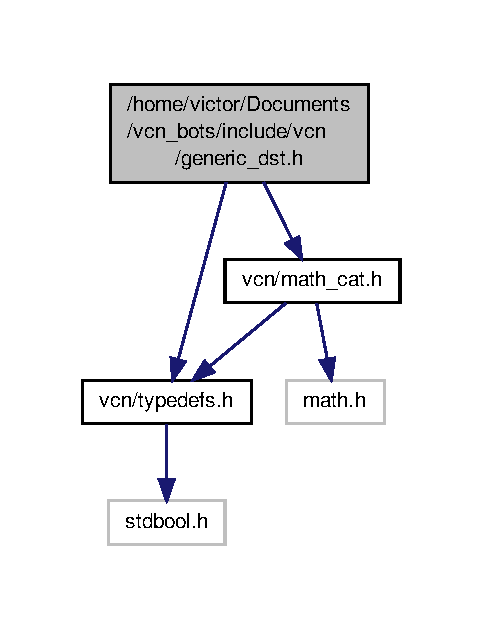
\includegraphics[width=232pt]{generic__dst_8h__incl}
\end{center}
\end{figure}
This graph shows which files directly or indirectly include this file\+:
\nopagebreak
\begin{figure}[H]
\begin{center}
\leavevmode
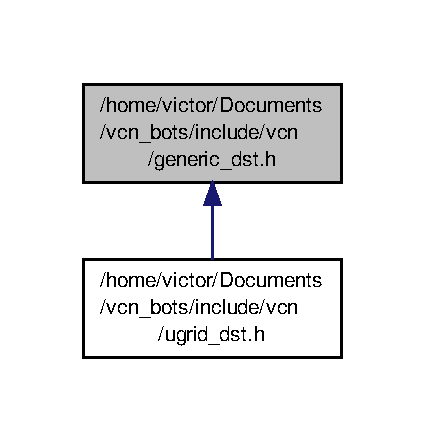
\includegraphics[width=204pt]{generic__dst_8h__dep__incl}
\end{center}
\end{figure}
\subsection*{Typedefs}
\begin{DoxyCompactItemize}
\item 
\hypertarget{generic__dst_8h_a2135b47b03a5f046d87fb039dd65c4ee}{typedef struct vcn\+\_\+list\+\_\+s {\bfseries vcn\+\_\+list\+\_\+t}}\label{generic__dst_8h_a2135b47b03a5f046d87fb039dd65c4ee}

\item 
\hypertarget{generic__dst_8h_a586be440648c1637b0acd4c6dd6e774f}{typedef struct vcn\+\_\+avl\+\_\+s {\bfseries vcn\+\_\+avl\+\_\+t}}\label{generic__dst_8h_a586be440648c1637b0acd4c6dd6e774f}

\item 
\hypertarget{generic__dst_8h_a7ae4f111e2f2ef0f3b753bee78c5de94}{typedef struct vcn\+\_\+htable\+\_\+s {\bfseries vcn\+\_\+htable\+\_\+t}}\label{generic__dst_8h_a7ae4f111e2f2ef0f3b753bee78c5de94}

\item 
\hypertarget{generic__dst_8h_a285b818de112b52cba94f1f93aaa5914}{typedef struct vcn\+\_\+list\+\_\+iter\+\_\+s {\bfseries vcn\+\_\+list\+\_\+iter\+\_\+t}}\label{generic__dst_8h_a285b818de112b52cba94f1f93aaa5914}

\item 
\hypertarget{generic__dst_8h_a52838d1595c1b877fbd8ad23c824707f}{typedef struct vcn\+\_\+avl\+\_\+iter\+\_\+s {\bfseries vcn\+\_\+avl\+\_\+iter\+\_\+t}}\label{generic__dst_8h_a52838d1595c1b877fbd8ad23c824707f}

\item 
\hypertarget{generic__dst_8h_a66ef2a7996969d813a7e11e0a920b80c}{typedef struct vcn\+\_\+htable\+\_\+iter\+\_\+s {\bfseries vcn\+\_\+htable\+\_\+iter\+\_\+t}}\label{generic__dst_8h_a66ef2a7996969d813a7e11e0a920b80c}

\end{DoxyCompactItemize}
\subsection*{Functions}
\begin{DoxyCompactItemize}
\item 
\hypertarget{generic__dst_8h_a56b46dd33f62f55de875c00c1dd18539}{vcn\+\_\+list\+\_\+t $\ast$ {\bfseries vcn\+\_\+list\+\_\+create} ()}\label{generic__dst_8h_a56b46dd33f62f55de875c00c1dd18539}

\item 
\hypertarget{generic__dst_8h_a82d90af53bbec4f26ff88edbff82b9da}{vcn\+\_\+list\+\_\+t $\ast$ {\bfseries vcn\+\_\+list\+\_\+clone} (const vcn\+\_\+list\+\_\+t $\ast$const list)}\label{generic__dst_8h_a82d90af53bbec4f26ff88edbff82b9da}

\item 
\hypertarget{generic__dst_8h_a4d9f14c6509ecae1b3e5f07148482b25}{void {\bfseries vcn\+\_\+list\+\_\+destroy} (vcn\+\_\+list\+\_\+t $\ast$list, void($\ast$free\+\_\+val)(void $\ast$))}\label{generic__dst_8h_a4d9f14c6509ecae1b3e5f07148482b25}

\item 
\hypertarget{generic__dst_8h_aa575a1afff9e0cc7b0ff47efc439cb42}{void {\bfseries vcn\+\_\+list\+\_\+clear} (vcn\+\_\+list\+\_\+t $\ast$list, void($\ast$free\+\_\+val)(void $\ast$))}\label{generic__dst_8h_aa575a1afff9e0cc7b0ff47efc439cb42}

\item 
\hypertarget{generic__dst_8h_afd9b18d30bfac43515650ca9f94879ea}{vcn\+\_\+list\+\_\+t $\ast$ {\bfseries vcn\+\_\+list\+\_\+create\+\_\+from\+\_\+array} (void $\ast$$\ast$array, uint N)}\label{generic__dst_8h_afd9b18d30bfac43515650ca9f94879ea}

\item 
\hypertarget{generic__dst_8h_a37d6ccd4320a8df1c8609e89c96bdb6d}{void $\ast$$\ast$ {\bfseries vcn\+\_\+list\+\_\+create\+\_\+array} (const vcn\+\_\+list\+\_\+t $\ast$const list)}\label{generic__dst_8h_a37d6ccd4320a8df1c8609e89c96bdb6d}

\item 
\hypertarget{generic__dst_8h_ad1217aed82b63ae1ba12123bda2d8475}{void {\bfseries vcn\+\_\+list\+\_\+insert} (vcn\+\_\+list\+\_\+t $\ast$const list, const void $\ast$const val)}\label{generic__dst_8h_ad1217aed82b63ae1ba12123bda2d8475}

\item 
\hypertarget{generic__dst_8h_a172eaecbe6dbe91dd7a964f02d347a2f}{void {\bfseries vcn\+\_\+list\+\_\+insert\+\_\+first} (vcn\+\_\+list\+\_\+t $\ast$list, const void $\ast$const val)}\label{generic__dst_8h_a172eaecbe6dbe91dd7a964f02d347a2f}

\item 
\hypertarget{generic__dst_8h_ab4e3360c92ce4e5f041933ea6923a918}{void $\ast$ {\bfseries vcn\+\_\+list\+\_\+remove\+\_\+first} (vcn\+\_\+list\+\_\+t $\ast$list)}\label{generic__dst_8h_ab4e3360c92ce4e5f041933ea6923a918}

\item 
\hypertarget{generic__dst_8h_a436e5c477d7c7ad7e6c59dba0aff90d4}{void $\ast$ {\bfseries vcn\+\_\+list\+\_\+remove\+\_\+last} (vcn\+\_\+list\+\_\+t $\ast$list)}\label{generic__dst_8h_a436e5c477d7c7ad7e6c59dba0aff90d4}

\item 
\hypertarget{generic__dst_8h_a9f948dfc247ebca987e8b09efd41f074}{void $\ast$ {\bfseries vcn\+\_\+list\+\_\+get\+\_\+first} (const vcn\+\_\+list\+\_\+t $\ast$const list)}\label{generic__dst_8h_a9f948dfc247ebca987e8b09efd41f074}

\item 
\hypertarget{generic__dst_8h_ad0d028e6a41423b9ffde9f48828838ed}{void $\ast$ {\bfseries vcn\+\_\+list\+\_\+get\+\_\+last} (const vcn\+\_\+list\+\_\+t $\ast$const list)}\label{generic__dst_8h_ad0d028e6a41423b9ffde9f48828838ed}

\item 
\hypertarget{generic__dst_8h_a63b43fb704dca9c2b98709ff528bb3cf}{void {\bfseries vcn\+\_\+list\+\_\+remove} (vcn\+\_\+list\+\_\+t $\ast$list, const void $\ast$const val)}\label{generic__dst_8h_a63b43fb704dca9c2b98709ff528bb3cf}

\item 
\hypertarget{generic__dst_8h_afe1022fc7ec87a8475e412097f9fa0de}{void $\ast$ {\bfseries vcn\+\_\+list\+\_\+exist} (const vcn\+\_\+list\+\_\+t $\ast$const list, const void $\ast$const val, int($\ast$compare)(const void $\ast$const, const void $\ast$const))}\label{generic__dst_8h_afe1022fc7ec87a8475e412097f9fa0de}

\item 
\hypertarget{generic__dst_8h_ad178fe72e608279bb8172b9f30406517}{uint {\bfseries vcn\+\_\+list\+\_\+get\+\_\+position} (const vcn\+\_\+list\+\_\+t $\ast$const list, const void $\ast$const val, int($\ast$compare)(const void $\ast$const, const void $\ast$const))}\label{generic__dst_8h_ad178fe72e608279bb8172b9f30406517}

\item 
\hypertarget{generic__dst_8h_abe2ce45e8911e2f9926332a43b946213}{uint {\bfseries vcn\+\_\+list\+\_\+length} (const vcn\+\_\+list\+\_\+t $\ast$const list)}\label{generic__dst_8h_abe2ce45e8911e2f9926332a43b946213}

\item 
\hypertarget{generic__dst_8h_a9985bd1188fdb0305748dcba187383d8}{vcn\+\_\+list\+\_\+iter\+\_\+t $\ast$ {\bfseries vcn\+\_\+list\+\_\+iter\+\_\+create} (const vcn\+\_\+list\+\_\+t $\ast$const list)}\label{generic__dst_8h_a9985bd1188fdb0305748dcba187383d8}

\item 
\hypertarget{generic__dst_8h_a8bdfeb8d01ce6d357814b7d611a89be0}{vcn\+\_\+list\+\_\+iter\+\_\+t $\ast$ {\bfseries vcn\+\_\+list\+\_\+iter\+\_\+clone} (const vcn\+\_\+list\+\_\+iter\+\_\+t $\ast$const iter)}\label{generic__dst_8h_a8bdfeb8d01ce6d357814b7d611a89be0}

\item 
\hypertarget{generic__dst_8h_a1fd0a37b4de8cda64ca061aa1b29393a}{void {\bfseries vcn\+\_\+list\+\_\+iter\+\_\+destroy} (vcn\+\_\+list\+\_\+iter\+\_\+t $\ast$iter)}\label{generic__dst_8h_a1fd0a37b4de8cda64ca061aa1b29393a}

\item 
\hypertarget{generic__dst_8h_a1ad6498126161220c06021299e469114}{void $\ast$ {\bfseries vcn\+\_\+list\+\_\+iter\+\_\+get\+\_\+next} (vcn\+\_\+list\+\_\+iter\+\_\+t $\ast$iter)}\label{generic__dst_8h_a1ad6498126161220c06021299e469114}

\item 
\hypertarget{generic__dst_8h_ae420c82f375c5a12415a1b448415065c}{bool {\bfseries vcn\+\_\+list\+\_\+iter\+\_\+has\+\_\+more} (vcn\+\_\+list\+\_\+iter\+\_\+t $\ast$iter)}\label{generic__dst_8h_ae420c82f375c5a12415a1b448415065c}

\item 
\hypertarget{generic__dst_8h_a683c23c16fb11ecb7f1fd47b96406bca}{void {\bfseries vcn\+\_\+list\+\_\+iter\+\_\+restart} (vcn\+\_\+list\+\_\+iter\+\_\+t $\ast$iter)}\label{generic__dst_8h_a683c23c16fb11ecb7f1fd47b96406bca}

\item 
\hypertarget{generic__dst_8h_a6edd29462169d518acca4640ba3932e1}{vcn\+\_\+avl\+\_\+t $\ast$ {\bfseries vcn\+\_\+avl\+\_\+create} (int($\ast$compare)(const void $\ast$const ,const void $\ast$const ))}\label{generic__dst_8h_a6edd29462169d518acca4640ba3932e1}

\item 
\hypertarget{generic__dst_8h_a9c957fd854c50620dad4cf5b2d5dc930}{vcn\+\_\+avl\+\_\+t $\ast$ {\bfseries vcn\+\_\+avl\+\_\+clone} (const vcn\+\_\+avl\+\_\+t $\ast$const avl)}\label{generic__dst_8h_a9c957fd854c50620dad4cf5b2d5dc930}

\item 
\hypertarget{generic__dst_8h_a198f8a041e468c64f22c80dc0611dbe6}{void {\bfseries vcn\+\_\+avl\+\_\+destroy} (vcn\+\_\+avl\+\_\+t $\ast$avl, void($\ast$free\+\_\+val)(void $\ast$))}\label{generic__dst_8h_a198f8a041e468c64f22c80dc0611dbe6}

\item 
\hypertarget{generic__dst_8h_a9d9fb67e6a76b243c75f839f59ec94f9}{void {\bfseries vcn\+\_\+avl\+\_\+clear} (vcn\+\_\+avl\+\_\+t $\ast$avl, void($\ast$free\+\_\+val)(void $\ast$))}\label{generic__dst_8h_a9d9fb67e6a76b243c75f839f59ec94f9}

\item 
\hypertarget{generic__dst_8h_a1d1ae51c6013f2e070882dade14fe4d4}{bool {\bfseries vcn\+\_\+avl\+\_\+insert} (vcn\+\_\+avl\+\_\+t $\ast$const avl, const void $\ast$const val)}\label{generic__dst_8h_a1d1ae51c6013f2e070882dade14fe4d4}

\item 
\hypertarget{generic__dst_8h_a847cd9e6b29818750541f8e7e367f706}{void $\ast$ {\bfseries vcn\+\_\+avl\+\_\+get\+\_\+most\+\_\+left} (const vcn\+\_\+avl\+\_\+t $\ast$const avl)}\label{generic__dst_8h_a847cd9e6b29818750541f8e7e367f706}

\item 
\hypertarget{generic__dst_8h_a7dff251c6fe787a553bf0ae66cd66bab}{void $\ast$ {\bfseries vcn\+\_\+avl\+\_\+get\+\_\+most\+\_\+right} (const vcn\+\_\+avl\+\_\+t $\ast$const avl)}\label{generic__dst_8h_a7dff251c6fe787a553bf0ae66cd66bab}

\item 
\hypertarget{generic__dst_8h_a1ca3d72a84ae3a000153a03d18f40bfb}{bool {\bfseries vcn\+\_\+avl\+\_\+remove} (vcn\+\_\+avl\+\_\+t $\ast$avl, void $\ast$val)}\label{generic__dst_8h_a1ca3d72a84ae3a000153a03d18f40bfb}

\item 
\hypertarget{generic__dst_8h_a8c93f772f8da90d6c1b737df8f53a47e}{void $\ast$ {\bfseries vcn\+\_\+avl\+\_\+remove\+\_\+most\+\_\+left} (vcn\+\_\+avl\+\_\+t $\ast$const avl)}\label{generic__dst_8h_a8c93f772f8da90d6c1b737df8f53a47e}

\item 
\hypertarget{generic__dst_8h_a763fd63e8381a57c3fb51506050ebf6c}{void $\ast$ {\bfseries vcn\+\_\+avl\+\_\+remove\+\_\+most\+\_\+right} (vcn\+\_\+avl\+\_\+t $\ast$const avl)}\label{generic__dst_8h_a763fd63e8381a57c3fb51506050ebf6c}

\item 
\hypertarget{generic__dst_8h_af736f770bbfd76511f46eb867d81cfed}{uint {\bfseries vcn\+\_\+avl\+\_\+length} (const vcn\+\_\+avl\+\_\+t $\ast$const avl)}\label{generic__dst_8h_af736f770bbfd76511f46eb867d81cfed}

\item 
\hypertarget{generic__dst_8h_a20dffbc3eaee0f8affa7f47595b16c83}{uint {\bfseries vcn\+\_\+avl\+\_\+height} (const vcn\+\_\+avl\+\_\+t $\ast$const avl)}\label{generic__dst_8h_a20dffbc3eaee0f8affa7f47595b16c83}

\item 
\hypertarget{generic__dst_8h_a5dfb553dbec4d82448331ccdbf2d2e51}{void $\ast$ {\bfseries vcn\+\_\+avl\+\_\+exist} (const vcn\+\_\+avl\+\_\+t $\ast$const avl, const void $\ast$const val)}\label{generic__dst_8h_a5dfb553dbec4d82448331ccdbf2d2e51}

\item 
\hypertarget{generic__dst_8h_a81296fb269a983bc3dd7d3ad600e4efe}{vcn\+\_\+avl\+\_\+iter\+\_\+t $\ast$ {\bfseries vcn\+\_\+avl\+\_\+iter\+\_\+create} (const vcn\+\_\+avl\+\_\+t $\ast$const avl)}\label{generic__dst_8h_a81296fb269a983bc3dd7d3ad600e4efe}

\item 
\hypertarget{generic__dst_8h_ad5a98f73eef80f557a89f15073bae387}{vcn\+\_\+avl\+\_\+iter\+\_\+t $\ast$ {\bfseries vcn\+\_\+avl\+\_\+iter\+\_\+clone} (const vcn\+\_\+avl\+\_\+iter\+\_\+t $\ast$const iter)}\label{generic__dst_8h_ad5a98f73eef80f557a89f15073bae387}

\item 
\hypertarget{generic__dst_8h_ac7c47bc5ba3e7972bc8f83d4227a7bdc}{void {\bfseries vcn\+\_\+avl\+\_\+iter\+\_\+destroy} (vcn\+\_\+avl\+\_\+iter\+\_\+t $\ast$iter)}\label{generic__dst_8h_ac7c47bc5ba3e7972bc8f83d4227a7bdc}

\item 
\hypertarget{generic__dst_8h_a94ef6711b0d5fe8f97f08cb0345769ec}{void $\ast$ {\bfseries vcn\+\_\+avl\+\_\+iter\+\_\+get\+\_\+next} (vcn\+\_\+avl\+\_\+iter\+\_\+t $\ast$iter)}\label{generic__dst_8h_a94ef6711b0d5fe8f97f08cb0345769ec}

\item 
\hypertarget{generic__dst_8h_a59dc0fbc96356eea3b1c942471f029b2}{bool {\bfseries vcn\+\_\+avl\+\_\+iter\+\_\+has\+\_\+more} (vcn\+\_\+avl\+\_\+iter\+\_\+t $\ast$iter)}\label{generic__dst_8h_a59dc0fbc96356eea3b1c942471f029b2}

\item 
\hypertarget{generic__dst_8h_afd25b371f81d633512b0d5dce09a0e61}{void {\bfseries vcn\+\_\+avl\+\_\+iter\+\_\+restart} (vcn\+\_\+avl\+\_\+iter\+\_\+t $\ast$iter)}\label{generic__dst_8h_afd25b371f81d633512b0d5dce09a0e61}

\item 
\hypertarget{generic__dst_8h_affcbfa3dc38700e0d78282e1ecef5692}{vcn\+\_\+htable\+\_\+t $\ast$ {\bfseries vcn\+\_\+htable\+\_\+create} (uint size, uint($\ast$hash\+\_\+key)(const void $\ast$const))}\label{generic__dst_8h_affcbfa3dc38700e0d78282e1ecef5692}

\item 
\hypertarget{generic__dst_8h_ac7ce8f4a82cf7450662eb448acccc09c}{void {\bfseries vcn\+\_\+htable\+\_\+destroy} (vcn\+\_\+htable\+\_\+t $\ast$htable, void($\ast$free\+\_\+val)(void $\ast$))}\label{generic__dst_8h_ac7ce8f4a82cf7450662eb448acccc09c}

\item 
\hypertarget{generic__dst_8h_a3f88de831b60aca9477ac21fdcc2549f}{void {\bfseries vcn\+\_\+htable\+\_\+clear} (vcn\+\_\+htable\+\_\+t $\ast$htable, void($\ast$free\+\_\+val)(void $\ast$))}\label{generic__dst_8h_a3f88de831b60aca9477ac21fdcc2549f}

\item 
\hypertarget{generic__dst_8h_a0cf077946b1753a53200d8b1c8c19771}{void {\bfseries vcn\+\_\+htable\+\_\+insert} (vcn\+\_\+htable\+\_\+t $\ast$htable, const void $\ast$const val)}\label{generic__dst_8h_a0cf077946b1753a53200d8b1c8c19771}

\item 
\hypertarget{generic__dst_8h_a2950717c202ddc0495452d9f255c648e}{void {\bfseries vcn\+\_\+htable\+\_\+remove} (vcn\+\_\+htable\+\_\+t $\ast$htable, const void $\ast$const val)}\label{generic__dst_8h_a2950717c202ddc0495452d9f255c648e}

\item 
\hypertarget{generic__dst_8h_ad824de6b046e1a6d3514534acb38eb2e}{void $\ast$ {\bfseries vcn\+\_\+htable\+\_\+remove\+\_\+first} (vcn\+\_\+htable\+\_\+t $\ast$htable)}\label{generic__dst_8h_ad824de6b046e1a6d3514534acb38eb2e}

\item 
\hypertarget{generic__dst_8h_a0198c0883e940c708e6d5b168fb692cd}{void $\ast$ {\bfseries vcn\+\_\+htable\+\_\+exist} (const vcn\+\_\+htable\+\_\+t $\ast$const htable, const void $\ast$const val, int($\ast$compare)(const void $\ast$const, const void $\ast$const))}\label{generic__dst_8h_a0198c0883e940c708e6d5b168fb692cd}

\item 
\hypertarget{generic__dst_8h_ae469eda3db836b4c7ced1c43ed92ec19}{uint {\bfseries vcn\+\_\+htable\+\_\+n\+\_\+hash\+\_\+collisions} (const vcn\+\_\+htable\+\_\+t $\ast$const htable)}\label{generic__dst_8h_ae469eda3db836b4c7ced1c43ed92ec19}

\item 
\hypertarget{generic__dst_8h_ae0ad9eafd5d33b3d625955ee4613bb52}{vcn\+\_\+list\+\_\+t $\ast$ {\bfseries vcn\+\_\+htable\+\_\+get\+\_\+hash\+\_\+collisions} (const vcn\+\_\+htable\+\_\+t $\ast$const htable)}\label{generic__dst_8h_ae0ad9eafd5d33b3d625955ee4613bb52}

\item 
\hypertarget{generic__dst_8h_a9b0f0e8b20a7e0924195f7182f93dba1}{uint {\bfseries vcn\+\_\+htable\+\_\+length} (vcn\+\_\+htable\+\_\+t $\ast$htable)}\label{generic__dst_8h_a9b0f0e8b20a7e0924195f7182f93dba1}

\item 
\hypertarget{generic__dst_8h_ad5dc8b6a398eca31922181342b8d2338}{uint {\bfseries vcn\+\_\+htable\+\_\+size} (vcn\+\_\+htable\+\_\+t $\ast$htable)}\label{generic__dst_8h_ad5dc8b6a398eca31922181342b8d2338}

\item 
\hypertarget{generic__dst_8h_aa52a1292f3fc65689aa3b26da2bd4399}{vcn\+\_\+htable\+\_\+iter\+\_\+t $\ast$ {\bfseries vcn\+\_\+htable\+\_\+iter\+\_\+create} (const vcn\+\_\+htable\+\_\+t $\ast$const htable)}\label{generic__dst_8h_aa52a1292f3fc65689aa3b26da2bd4399}

\item 
\hypertarget{generic__dst_8h_a1b3c88c028959be59a6f85f2dd5992a8}{void {\bfseries vcn\+\_\+htable\+\_\+iter\+\_\+destroy} (vcn\+\_\+htable\+\_\+iter\+\_\+t $\ast$iter)}\label{generic__dst_8h_a1b3c88c028959be59a6f85f2dd5992a8}

\item 
\hypertarget{generic__dst_8h_aea485ba6605d82f95dafae28d99212f0}{void $\ast$ {\bfseries vcn\+\_\+htable\+\_\+iter\+\_\+get\+\_\+next} (vcn\+\_\+htable\+\_\+iter\+\_\+t $\ast$iter)}\label{generic__dst_8h_aea485ba6605d82f95dafae28d99212f0}

\item 
\hypertarget{generic__dst_8h_aee50096d7fe45b71bfc8b23ad7d1b525}{bool {\bfseries vcn\+\_\+htable\+\_\+iter\+\_\+has\+\_\+more} (vcn\+\_\+htable\+\_\+iter\+\_\+t $\ast$iter)}\label{generic__dst_8h_aee50096d7fe45b71bfc8b23ad7d1b525}

\item 
\hypertarget{generic__dst_8h_a535d17a8edb92c06ebf9adaa1bed90ce}{void {\bfseries vcn\+\_\+htable\+\_\+iter\+\_\+notify\+\_\+element\+\_\+to\+\_\+remove} (vcn\+\_\+htable\+\_\+iter\+\_\+t $\ast$iter, void $\ast$elem)}\label{generic__dst_8h_a535d17a8edb92c06ebf9adaa1bed90ce}

\item 
\hypertarget{generic__dst_8h_a8fa8dcb9fd1886c3b1e768f4321b4303}{void {\bfseries vcn\+\_\+htable\+\_\+iter\+\_\+restart} (vcn\+\_\+htable\+\_\+iter\+\_\+t $\ast$iter)}\label{generic__dst_8h_a8fa8dcb9fd1886c3b1e768f4321b4303}

\end{DoxyCompactItemize}


\subsection{Detailed Description}
General purpose data structures. 

\begin{DoxyAuthor}{Author}
Victor Eduardo Cardoso Nungaray ~\newline
 victorc@cimat.\+mx ~\newline
 \href{https://twitter.com/victore_cardoso}{\tt @victore\+\_\+cardoso } 
\end{DoxyAuthor}
\begin{DoxyDate}{Date}
10 August 2015
\end{DoxyDate}
\begin{DoxyParagraph}{License\+:}
This piece of code is in the P\+U\+B\+L\+I\+C D\+O\+M\+A\+I\+N, if your government does not recognizes such a dedication, then you are granted a perpetual and irrevocable license to copy and modify this file however you want. This does not imply any warranty. ~\newline
 Attributions and feedback are always welcome. 
\end{DoxyParagraph}

\hypertarget{geometric__bot-cairo_8h}{\section{/home/victor/\+Documents/vcn\+\_\+bots/include/vcn/geometric\+\_\+bot-\/cairo.h File Reference}
\label{geometric__bot-cairo_8h}\index{/home/victor/\+Documents/vcn\+\_\+bots/include/vcn/geometric\+\_\+bot-\/cairo.\+h@{/home/victor/\+Documents/vcn\+\_\+bots/include/vcn/geometric\+\_\+bot-\/cairo.\+h}}
}


Drawing functions using \href{http://www.cairographics.org}{\tt Cairo Graphics Library}.  


{\ttfamily \#include $<$cairo.\+h$>$}\\*
{\ttfamily \#include \char`\"{}vcn/typedefs.\+h\char`\"{}}\\*
{\ttfamily \#include \char`\"{}vcn/geometric\+\_\+bot.\+h\char`\"{}}\\*
Include dependency graph for geometric\+\_\+bot-\/cairo.h\+:
\nopagebreak
\begin{figure}[H]
\begin{center}
\leavevmode
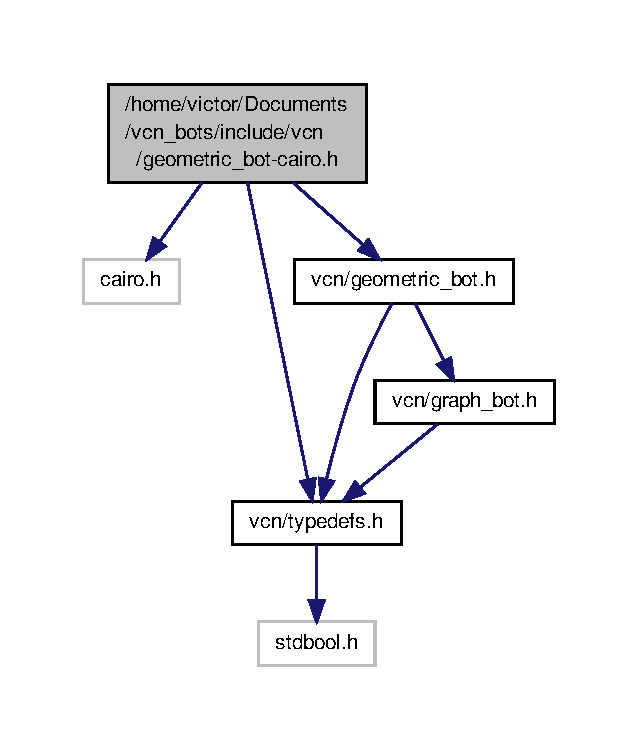
\includegraphics[width=306pt]{geometric__bot-cairo_8h__incl}
\end{center}
\end{figure}
\subsection*{Functions}
\begin{DoxyCompactItemize}
\item 
void \hyperlink{geometric__bot-cairo_8h_a3b8ba617ef66d703239f5eb74487971a}{vcn\+\_\+model\+\_\+export\+\_\+png} (const \hyperlink{geometric__bot_8h_a10375cbf3125046dc59bd4bef92432ad}{vcn\+\_\+model\+\_\+t} $\ast$const model, const char $\ast$filename, int width, int height, bool include\+\_\+numbering)
\begin{DoxyCompactList}\small\item\em Export a P\+N\+G image of the model. \end{DoxyCompactList}\item 
void \hyperlink{geometric__bot-cairo_8h_aff415fd425c1c8a60322e5eb45749ee0}{vcn\+\_\+model\+\_\+export\+\_\+eps} (const \hyperlink{geometric__bot_8h_a10375cbf3125046dc59bd4bef92432ad}{vcn\+\_\+model\+\_\+t} $\ast$const model, const char $\ast$filename, int width, int height, bool include\+\_\+numbering)
\begin{DoxyCompactList}\small\item\em Export an E\+P\+S image of the model. \end{DoxyCompactList}\item 
void \hyperlink{geometric__bot-cairo_8h_a404bf8be5f7e93e864721274dfaa4b69}{vcn\+\_\+mesh\+\_\+save\+\_\+png} (const \hyperlink{geometric__bot_8h_a8942da13867aa76dd55d8f2b079ad3ce}{vcn\+\_\+mesh\+\_\+t} $\ast$const mesh, const char $\ast$filename, int width, int height)
\begin{DoxyCompactList}\small\item\em Export a P\+N\+G image of the mesh. \end{DoxyCompactList}\item 
void \hyperlink{geometric__bot-cairo_8h_aab095b139981821f1d079e7da88102e8}{vcn\+\_\+mesh\+\_\+save\+\_\+eps} (const \hyperlink{geometric__bot_8h_a8942da13867aa76dd55d8f2b079ad3ce}{vcn\+\_\+mesh\+\_\+t} $\ast$const mesh, const char $\ast$filename, int width, int height)
\begin{DoxyCompactList}\small\item\em Export an E\+P\+S image of the mesh. \end{DoxyCompactList}\item 
void \hyperlink{geometric__bot-cairo_8h_aa096a0bdddf902a0cf2380d6397e8e4e}{vcn\+\_\+msh3trg\+\_\+save\+\_\+png} (const \hyperlink{geometric__bot_8h_af753a8fb5e30b4d81a02489e92b54df2}{vcn\+\_\+msh3trg\+\_\+t} $\ast$const msh3trg, const char $\ast$filename, int width, int height, double rgba\+\_\+bg\mbox{[}4\mbox{]}, double rgba\+\_\+fg\mbox{[}4\mbox{]}, double rgb\+\_\+edge\mbox{[}3\mbox{]}, double rgb\+\_\+sgm\mbox{[}3\mbox{]}, double edge\+\_\+width, double sgm\+\_\+width)
\begin{DoxyCompactList}\small\item\em Export a P\+N\+G image of the triangulation. \end{DoxyCompactList}\item 
void \hyperlink{geometric__bot-cairo_8h_ae1ddaf8105a328f7c74387319007a87b}{vcn\+\_\+msh3trg\+\_\+partition\+\_\+save\+\_\+png} (const \hyperlink{geometric__bot_8h_af753a8fb5e30b4d81a02489e92b54df2}{vcn\+\_\+msh3trg\+\_\+t} $\ast$const msh3trg, const char $\ast$filename, int width, int height, uint k\+\_\+part, const uint $\ast$const part, uint k\+\_\+to\+\_\+draw, double scale\+\_\+partitions, double rgba\+\_\+bg\mbox{[}4\mbox{]}, double alpha\+\_\+fg, double rgb\+\_\+edge\mbox{[}3\mbox{]}, double rgb\+\_\+sgm\mbox{[}3\mbox{]}, double edge\+\_\+width, double sgm\+\_\+width)
\begin{DoxyCompactList}\small\item\em Export a P\+N\+G image of the triangulation and its partitions. \end{DoxyCompactList}\item 
void \hyperlink{geometric__bot-cairo_8h_ad4ac0d9c4ad1f317494ab7314317eb1a}{vcn\+\_\+mshpoly\+\_\+save\+\_\+png} (const \hyperlink{geometric__bot_8h_a25e055df6f6e0902c79e1f37ef4cc329}{vcn\+\_\+mshpoly\+\_\+t} $\ast$const mshpoly, char $\ast$filename, bool draw\+\_\+adjacencies, int width, int height)
\begin{DoxyCompactList}\small\item\em Export a P\+N\+G image of the Voronoi graph. \end{DoxyCompactList}\item 
void \hyperlink{geometric__bot-cairo_8h_a2c2aafbd20b8706da1213271dc086be5}{vcn\+\_\+mshpack\+\_\+save\+\_\+png} (const \hyperlink{geometric__bot_8h_aa1e47f3fc55677e96c43ca151d971d86}{vcn\+\_\+mshpack\+\_\+t} $\ast$const mshpack, const char $\ast$filename, int width, int height)
\begin{DoxyCompactList}\small\item\em Export a P\+N\+G image of the sphere-\/pack. \end{DoxyCompactList}\end{DoxyCompactItemize}


\subsection{Detailed Description}
Drawing functions using \href{http://www.cairographics.org}{\tt Cairo Graphics Library}. 

\begin{DoxyAuthor}{Author}
Victor Eduardo Cardoso Nungaray ~\newline
 victorc@cimat.\+mx ~\newline
 \href{https://twitter.com/victore_cardoso}{\tt @victore\+\_\+cardoso } 
\end{DoxyAuthor}
\begin{DoxyDate}{Date}
4 August 2015
\end{DoxyDate}
\begin{DoxyParagraph}{License\+:}
This piece of code is in the P\+U\+B\+L\+I\+C D\+O\+M\+A\+I\+N, if your government does not recognizes such a dedication, then you are granted a perpetual and irrevocable license to copy and modify this file however you want. This does not imply any warranty. ~\newline
 Attributions and feedback are always welcome. 
\end{DoxyParagraph}


\subsection{Function Documentation}
\hypertarget{geometric__bot-cairo_8h_aab095b139981821f1d079e7da88102e8}{\index{geometric\+\_\+bot-\/cairo.\+h@{geometric\+\_\+bot-\/cairo.\+h}!vcn\+\_\+mesh\+\_\+save\+\_\+eps@{vcn\+\_\+mesh\+\_\+save\+\_\+eps}}
\index{vcn\+\_\+mesh\+\_\+save\+\_\+eps@{vcn\+\_\+mesh\+\_\+save\+\_\+eps}!geometric\+\_\+bot-\/cairo.\+h@{geometric\+\_\+bot-\/cairo.\+h}}
\subsubsection[{vcn\+\_\+mesh\+\_\+save\+\_\+eps}]{\setlength{\rightskip}{0pt plus 5cm}void vcn\+\_\+mesh\+\_\+save\+\_\+eps (
\begin{DoxyParamCaption}
\item[{const {\bf vcn\+\_\+mesh\+\_\+t} $\ast$const}]{mesh, }
\item[{const char $\ast$}]{filename, }
\item[{int}]{width, }
\item[{int}]{height}
\end{DoxyParamCaption}
)}}\label{geometric__bot-cairo_8h_aab095b139981821f1d079e7da88102e8}


Export an E\+P\+S image of the mesh. 


\begin{DoxyParams}[1]{Parameters}
\mbox{\tt in}  & {\em mesh} & Mesh to be displayed in the image. \\
\hline
\mbox{\tt in}  & {\em filename} & Name of the P\+N\+G file. \\
\hline
\mbox{\tt in}  & {\em width} & Width of the image. \\
\hline
\mbox{\tt in}  & {\em height} & of the image. \\
\hline
\end{DoxyParams}
\hypertarget{geometric__bot-cairo_8h_a404bf8be5f7e93e864721274dfaa4b69}{\index{geometric\+\_\+bot-\/cairo.\+h@{geometric\+\_\+bot-\/cairo.\+h}!vcn\+\_\+mesh\+\_\+save\+\_\+png@{vcn\+\_\+mesh\+\_\+save\+\_\+png}}
\index{vcn\+\_\+mesh\+\_\+save\+\_\+png@{vcn\+\_\+mesh\+\_\+save\+\_\+png}!geometric\+\_\+bot-\/cairo.\+h@{geometric\+\_\+bot-\/cairo.\+h}}
\subsubsection[{vcn\+\_\+mesh\+\_\+save\+\_\+png}]{\setlength{\rightskip}{0pt plus 5cm}void vcn\+\_\+mesh\+\_\+save\+\_\+png (
\begin{DoxyParamCaption}
\item[{const {\bf vcn\+\_\+mesh\+\_\+t} $\ast$const}]{mesh, }
\item[{const char $\ast$}]{filename, }
\item[{int}]{width, }
\item[{int}]{height}
\end{DoxyParamCaption}
)}}\label{geometric__bot-cairo_8h_a404bf8be5f7e93e864721274dfaa4b69}


Export a P\+N\+G image of the mesh. 


\begin{DoxyParams}[1]{Parameters}
\mbox{\tt in}  & {\em mesh} & Mesh to be displayed in the image. \\
\hline
\mbox{\tt in}  & {\em filename} & Name of the P\+N\+G file. \\
\hline
\mbox{\tt in}  & {\em width} & Width of the image. \\
\hline
\mbox{\tt in}  & {\em height} & of the image. \\
\hline
\end{DoxyParams}
\hypertarget{geometric__bot-cairo_8h_aff415fd425c1c8a60322e5eb45749ee0}{\index{geometric\+\_\+bot-\/cairo.\+h@{geometric\+\_\+bot-\/cairo.\+h}!vcn\+\_\+model\+\_\+export\+\_\+eps@{vcn\+\_\+model\+\_\+export\+\_\+eps}}
\index{vcn\+\_\+model\+\_\+export\+\_\+eps@{vcn\+\_\+model\+\_\+export\+\_\+eps}!geometric\+\_\+bot-\/cairo.\+h@{geometric\+\_\+bot-\/cairo.\+h}}
\subsubsection[{vcn\+\_\+model\+\_\+export\+\_\+eps}]{\setlength{\rightskip}{0pt plus 5cm}void vcn\+\_\+model\+\_\+export\+\_\+eps (
\begin{DoxyParamCaption}
\item[{const {\bf vcn\+\_\+model\+\_\+t} $\ast$const}]{model, }
\item[{const char $\ast$}]{filename, }
\item[{int}]{width, }
\item[{int}]{height, }
\item[{bool}]{include\+\_\+numbering}
\end{DoxyParamCaption}
)}}\label{geometric__bot-cairo_8h_aff415fd425c1c8a60322e5eb45749ee0}


Export an E\+P\+S image of the model. 


\begin{DoxyParams}[1]{Parameters}
\mbox{\tt in}  & {\em model} & Model to be displayed in the image. \\
\hline
\mbox{\tt in}  & {\em filename} & Name of the E\+P\+S file. \\
\hline
\mbox{\tt in}  & {\em width} & Width of the image. \\
\hline
\mbox{\tt in}  & {\em height} & of the image. \\
\hline
\mbox{\tt in}  & {\em include\+\_\+numbering} & Enable or Disable the ids of vertices and segments. \\
\hline
\end{DoxyParams}
\hypertarget{geometric__bot-cairo_8h_a3b8ba617ef66d703239f5eb74487971a}{\index{geometric\+\_\+bot-\/cairo.\+h@{geometric\+\_\+bot-\/cairo.\+h}!vcn\+\_\+model\+\_\+export\+\_\+png@{vcn\+\_\+model\+\_\+export\+\_\+png}}
\index{vcn\+\_\+model\+\_\+export\+\_\+png@{vcn\+\_\+model\+\_\+export\+\_\+png}!geometric\+\_\+bot-\/cairo.\+h@{geometric\+\_\+bot-\/cairo.\+h}}
\subsubsection[{vcn\+\_\+model\+\_\+export\+\_\+png}]{\setlength{\rightskip}{0pt plus 5cm}void vcn\+\_\+model\+\_\+export\+\_\+png (
\begin{DoxyParamCaption}
\item[{const {\bf vcn\+\_\+model\+\_\+t} $\ast$const}]{model, }
\item[{const char $\ast$}]{filename, }
\item[{int}]{width, }
\item[{int}]{height, }
\item[{bool}]{include\+\_\+numbering}
\end{DoxyParamCaption}
)}}\label{geometric__bot-cairo_8h_a3b8ba617ef66d703239f5eb74487971a}


Export a P\+N\+G image of the model. 


\begin{DoxyParams}[1]{Parameters}
\mbox{\tt in}  & {\em model} & Model to be displayed in the image. \\
\hline
\mbox{\tt in}  & {\em filename} & Name of the P\+N\+G file. \\
\hline
\mbox{\tt in}  & {\em width} & Width of the image. \\
\hline
\mbox{\tt in}  & {\em height} & of the image. \\
\hline
\mbox{\tt in}  & {\em include\+\_\+numbering} & Enable or Disable the ids of vertices and segments. \\
\hline
\end{DoxyParams}
\hypertarget{geometric__bot-cairo_8h_ae1ddaf8105a328f7c74387319007a87b}{\index{geometric\+\_\+bot-\/cairo.\+h@{geometric\+\_\+bot-\/cairo.\+h}!vcn\+\_\+msh3trg\+\_\+partition\+\_\+save\+\_\+png@{vcn\+\_\+msh3trg\+\_\+partition\+\_\+save\+\_\+png}}
\index{vcn\+\_\+msh3trg\+\_\+partition\+\_\+save\+\_\+png@{vcn\+\_\+msh3trg\+\_\+partition\+\_\+save\+\_\+png}!geometric\+\_\+bot-\/cairo.\+h@{geometric\+\_\+bot-\/cairo.\+h}}
\subsubsection[{vcn\+\_\+msh3trg\+\_\+partition\+\_\+save\+\_\+png}]{\setlength{\rightskip}{0pt plus 5cm}void vcn\+\_\+msh3trg\+\_\+partition\+\_\+save\+\_\+png (
\begin{DoxyParamCaption}
\item[{const {\bf vcn\+\_\+msh3trg\+\_\+t} $\ast$const}]{msh3trg, }
\item[{const char $\ast$}]{filename, }
\item[{int}]{width, }
\item[{int}]{height, }
\item[{uint}]{k\+\_\+part, }
\item[{const uint $\ast$const}]{part, }
\item[{uint}]{k\+\_\+to\+\_\+draw, }
\item[{double}]{scale\+\_\+partitions, }
\item[{double}]{rgba\+\_\+bg\mbox{[}4\mbox{]}, }
\item[{double}]{alpha\+\_\+fg, }
\item[{double}]{rgb\+\_\+edge\mbox{[}3\mbox{]}, }
\item[{double}]{rgb\+\_\+sgm\mbox{[}3\mbox{]}, }
\item[{double}]{edge\+\_\+width, }
\item[{double}]{sgm\+\_\+width}
\end{DoxyParamCaption}
)}}\label{geometric__bot-cairo_8h_ae1ddaf8105a328f7c74387319007a87b}


Export a P\+N\+G image of the triangulation and its partitions. 


\begin{DoxyParams}[1]{Parameters}
\mbox{\tt in}  & {\em msh3trg} & Triangulation to be displayed. \\
\hline
\mbox{\tt in}  & {\em k\+\_\+part} & Number of partitions. \\
\hline
\mbox{\tt in}  & {\em part} & Partition corresponding to the vertex. \\
\hline
\mbox{\tt in}  & {\em filename} & Name of the image file. \\
\hline
\mbox{\tt in}  & {\em width} & Image width. \\
\hline
\mbox{\tt in}  & {\em height} & Image height. \\
\hline
\mbox{\tt in}  & {\em k\+\_\+to\+\_\+draw} & Partition to draw. Zero to draw all of them. \\
\hline
\mbox{\tt in}  & {\em scale\+\_\+partitions} & Scale of the size of the partitions, in (0,1\mbox{]}. \\
\hline
\mbox{\tt in}  & {\em rgba\+\_\+bg} & Background color, N\+U\+L\+L to set white. ~\newline
 Color channels\+: Red, Green, Blue and Alpha. \\
\hline
\mbox{\tt in}  & {\em alpha\+\_\+fg} & Alpha channel for triangles color. ~\newline
 Color channels\+: Red, Green, Blue and Alpha. \\
\hline
\mbox{\tt in}  & {\em rgb\+\_\+edge} & Edges line color, N\+U\+L\+L to set default color. ~\newline
 Color channels\+: Red, Green and Blue. \\
\hline
\mbox{\tt in}  & {\em rgb\+\_\+sgm} & Segments line color, N\+U\+L\+L to set default color. ~\newline
 Color channels\+: Red, Green and Blue. \\
\hline
\mbox{\tt in}  & {\em edge\+\_\+width} & Line width to draw edges. \\
\hline
\mbox{\tt in}  & {\em sgm\+\_\+width} & Line width to draw input segments. \\
\hline
\end{DoxyParams}
\hypertarget{geometric__bot-cairo_8h_aa096a0bdddf902a0cf2380d6397e8e4e}{\index{geometric\+\_\+bot-\/cairo.\+h@{geometric\+\_\+bot-\/cairo.\+h}!vcn\+\_\+msh3trg\+\_\+save\+\_\+png@{vcn\+\_\+msh3trg\+\_\+save\+\_\+png}}
\index{vcn\+\_\+msh3trg\+\_\+save\+\_\+png@{vcn\+\_\+msh3trg\+\_\+save\+\_\+png}!geometric\+\_\+bot-\/cairo.\+h@{geometric\+\_\+bot-\/cairo.\+h}}
\subsubsection[{vcn\+\_\+msh3trg\+\_\+save\+\_\+png}]{\setlength{\rightskip}{0pt plus 5cm}void vcn\+\_\+msh3trg\+\_\+save\+\_\+png (
\begin{DoxyParamCaption}
\item[{const {\bf vcn\+\_\+msh3trg\+\_\+t} $\ast$const}]{msh3trg, }
\item[{const char $\ast$}]{filename, }
\item[{int}]{width, }
\item[{int}]{height, }
\item[{double}]{rgba\+\_\+bg\mbox{[}4\mbox{]}, }
\item[{double}]{rgba\+\_\+fg\mbox{[}4\mbox{]}, }
\item[{double}]{rgb\+\_\+edge\mbox{[}3\mbox{]}, }
\item[{double}]{rgb\+\_\+sgm\mbox{[}3\mbox{]}, }
\item[{double}]{edge\+\_\+width, }
\item[{double}]{sgm\+\_\+width}
\end{DoxyParamCaption}
)}}\label{geometric__bot-cairo_8h_aa096a0bdddf902a0cf2380d6397e8e4e}


Export a P\+N\+G image of the triangulation. 


\begin{DoxyParams}[1]{Parameters}
\mbox{\tt in}  & {\em msh3trg} & Triangulation to be displayed. \\
\hline
\mbox{\tt in}  & {\em filename} & Name of the image file. \\
\hline
\mbox{\tt in}  & {\em width} & Image width. \\
\hline
\mbox{\tt in}  & {\em height} & Image height. \\
\hline
\mbox{\tt in}  & {\em rgba\+\_\+bg} & Background color, N\+U\+L\+L to set white. ~\newline
 Color channels\+: Red, Green, Blue and Alpha. \\
\hline
\mbox{\tt in}  & {\em rgba\+\_\+fg} & Triangles color, N\+U\+L\+L to set default color. ~\newline
 Color channels\+: Red, Green, Blue and Alpha. \\
\hline
\mbox{\tt in}  & {\em rgb\+\_\+edge} & Edges line color, N\+U\+L\+L to set default color. ~\newline
 Color channels\+: Red, Green and Blue. \\
\hline
\mbox{\tt in}  & {\em rgb\+\_\+sgm} & Segments line color, N\+U\+L\+L to set default color. ~\newline
 Color channels\+: Red, Green and Blue. \\
\hline
\mbox{\tt in}  & {\em edge\+\_\+width} & Line width to draw edges. \\
\hline
\mbox{\tt in}  & {\em sgm\+\_\+width} & Line width to draw input segments. \\
\hline
\end{DoxyParams}
\hypertarget{geometric__bot-cairo_8h_a2c2aafbd20b8706da1213271dc086be5}{\index{geometric\+\_\+bot-\/cairo.\+h@{geometric\+\_\+bot-\/cairo.\+h}!vcn\+\_\+mshpack\+\_\+save\+\_\+png@{vcn\+\_\+mshpack\+\_\+save\+\_\+png}}
\index{vcn\+\_\+mshpack\+\_\+save\+\_\+png@{vcn\+\_\+mshpack\+\_\+save\+\_\+png}!geometric\+\_\+bot-\/cairo.\+h@{geometric\+\_\+bot-\/cairo.\+h}}
\subsubsection[{vcn\+\_\+mshpack\+\_\+save\+\_\+png}]{\setlength{\rightskip}{0pt plus 5cm}void vcn\+\_\+mshpack\+\_\+save\+\_\+png (
\begin{DoxyParamCaption}
\item[{const {\bf vcn\+\_\+mshpack\+\_\+t} $\ast$const}]{mshpack, }
\item[{const char $\ast$}]{filename, }
\item[{int}]{width, }
\item[{int}]{height}
\end{DoxyParamCaption}
)}}\label{geometric__bot-cairo_8h_a2c2aafbd20b8706da1213271dc086be5}


Export a P\+N\+G image of the sphere-\/pack. 


\begin{DoxyParams}[1]{Parameters}
\mbox{\tt in}  & {\em mshpack} & Sphere-\/pack to be displayed. \\
\hline
\mbox{\tt in}  & {\em filename} & Name of the image file. \\
\hline
\mbox{\tt in}  & {\em width} & Image width. \\
\hline
\mbox{\tt in}  & {\em height} & Image height. \\
\hline
\end{DoxyParams}
\hypertarget{geometric__bot-cairo_8h_ad4ac0d9c4ad1f317494ab7314317eb1a}{\index{geometric\+\_\+bot-\/cairo.\+h@{geometric\+\_\+bot-\/cairo.\+h}!vcn\+\_\+mshpoly\+\_\+save\+\_\+png@{vcn\+\_\+mshpoly\+\_\+save\+\_\+png}}
\index{vcn\+\_\+mshpoly\+\_\+save\+\_\+png@{vcn\+\_\+mshpoly\+\_\+save\+\_\+png}!geometric\+\_\+bot-\/cairo.\+h@{geometric\+\_\+bot-\/cairo.\+h}}
\subsubsection[{vcn\+\_\+mshpoly\+\_\+save\+\_\+png}]{\setlength{\rightskip}{0pt plus 5cm}void vcn\+\_\+mshpoly\+\_\+save\+\_\+png (
\begin{DoxyParamCaption}
\item[{const {\bf vcn\+\_\+mshpoly\+\_\+t} $\ast$const}]{mshpoly, }
\item[{char $\ast$}]{filename, }
\item[{bool}]{draw\+\_\+adjacencies, }
\item[{int}]{width, }
\item[{int}]{height}
\end{DoxyParamCaption}
)}}\label{geometric__bot-cairo_8h_ad4ac0d9c4ad1f317494ab7314317eb1a}


Export a P\+N\+G image of the Voronoi graph. 


\begin{DoxyParams}[1]{Parameters}
\mbox{\tt in}  & {\em mshpoly} & Voronoi graph to be displayed. \\
\hline
\mbox{\tt in}  & {\em filename} & Name of the image file. \\
\hline
\mbox{\tt in}  & {\em draw\+\_\+adjacencies} & Enable or disable drawing adjacencies. \\
\hline
\mbox{\tt in}  & {\em width} & Image width. \\
\hline
\mbox{\tt in}  & {\em height} & Image height. \\
\hline
\end{DoxyParams}

\hypertarget{geometric__bot-coming__soon_8h}{\section{/home/victor/\+Documents/vcn\+\_\+bots/include/vcn/geometric\+\_\+bot-\/coming\+\_\+soon.h File Reference}
\label{geometric__bot-coming__soon_8h}\index{/home/victor/\+Documents/vcn\+\_\+bots/include/vcn/geometric\+\_\+bot-\/coming\+\_\+soon.\+h@{/home/victor/\+Documents/vcn\+\_\+bots/include/vcn/geometric\+\_\+bot-\/coming\+\_\+soon.\+h}}
}


Features to be added in the next release.  


{\ttfamily \#include $<$stdbool.\+h$>$}\\*
Include dependency graph for geometric\+\_\+bot-\/coming\+\_\+soon.h\+:
\nopagebreak
\begin{figure}[H]
\begin{center}
\leavevmode
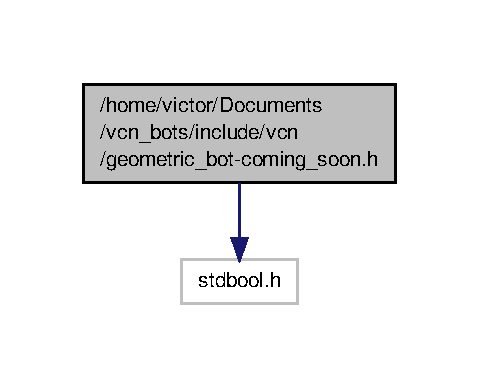
\includegraphics[width=230pt]{geometric__bot-coming__soon_8h__incl}
\end{center}
\end{figure}
\subsection*{Classes}
\begin{DoxyCompactItemize}
\item 
struct \hyperlink{structvcn__mshqmix__s}{vcn\+\_\+mshqmix\+\_\+s}
\begin{DoxyCompactList}\small\item\em Read-\/only mesh structure conformed by triangles and quadrilaterals. Such a mesh is produced by joining couples of triangles which maximizes the quality of the quadrilateral formed, using a greedy strategy. \end{DoxyCompactList}\item 
struct \hyperlink{structvcn__mshquad__s}{vcn\+\_\+mshquad\+\_\+s}
\begin{DoxyCompactList}\small\item\em Read-\/only structure storing a mesh of quadrilaterals, which is the result of a perfect matching of couples of triangles maximizing the global quality of quadrilaterals, without leaving isolated triangles in the mesh. \end{DoxyCompactList}\end{DoxyCompactItemize}
\subsection*{Typedefs}
\begin{DoxyCompactItemize}
\item 
\hypertarget{geometric__bot-coming__soon_8h_a6afc4193e3c1f85a155299aaafc942e7}{typedef struct \hyperlink{structvcn__mshqmix__s}{vcn\+\_\+mshqmix\+\_\+s} \hyperlink{geometric__bot-coming__soon_8h_a6afc4193e3c1f85a155299aaafc942e7}{vcn\+\_\+mshqmix\+\_\+t}}\label{geometric__bot-coming__soon_8h_a6afc4193e3c1f85a155299aaafc942e7}

\begin{DoxyCompactList}\small\item\em Read-\/only mesh structure conformed by triangles and quadrilaterals. Such a mesh is produced by joining couples of triangles which maximizes the quality of the quadrilateral formed, using a greedy strategy. \end{DoxyCompactList}\item 
\hypertarget{geometric__bot-coming__soon_8h_ad8d160c4087aa79eaa0a4cd72fba2b67}{typedef struct \hyperlink{structvcn__mshquad__s}{vcn\+\_\+mshquad\+\_\+s} \hyperlink{geometric__bot-coming__soon_8h_ad8d160c4087aa79eaa0a4cd72fba2b67}{vcn\+\_\+mshquad\+\_\+t}}\label{geometric__bot-coming__soon_8h_ad8d160c4087aa79eaa0a4cd72fba2b67}

\begin{DoxyCompactList}\small\item\em Read-\/only structure storing a mesh of quadrilaterals, which is the result of a perfect matching of couples of triangles maximizing the global quality of quadrilaterals, without leaving isolated triangles in the mesh. \end{DoxyCompactList}\end{DoxyCompactItemize}


\subsection{Detailed Description}
Features to be added in the next release. 

\begin{DoxyAuthor}{Author}
Victor Eduardo Cardoso Nungaray ~\newline
 victorc@cimat.\+mx ~\newline
 \href{https://twitter.com/victore_cardoso}{\tt @victore\+\_\+cardoso } 
\end{DoxyAuthor}
\begin{DoxyDate}{Date}
5 August 2015
\end{DoxyDate}
\begin{DoxyParagraph}{License\+:}
This piece of code is in the P\+U\+B\+L\+I\+C D\+O\+M\+A\+I\+N, if your government does not recognizes such a dedication, then you are granted a perpetual and irrevocable license to copy and modify this file however you want. This does not imply any warranty. ~\newline
 Attributions and feedback are always welcome. 
\end{DoxyParagraph}

\hypertarget{geometric__bot_8h}{\section{/home/victor/\+Documents/vcn\+\_\+bots/include/vcn/geometric\+\_\+bot.h File Reference}
\label{geometric__bot_8h}\index{/home/victor/\+Documents/vcn\+\_\+bots/include/vcn/geometric\+\_\+bot.\+h@{/home/victor/\+Documents/vcn\+\_\+bots/include/vcn/geometric\+\_\+bot.\+h}}
}


The geometric bot is a program used to generate tesselations, such as meshes suited for numerical interpolation in a wide range of engineering applications, such as computer graphics, finite element, computer vision and machine learning.  


{\ttfamily \#include \char`\"{}vcn/typedefs.\+h\char`\"{}}\\*
{\ttfamily \#include \char`\"{}vcn/graph\+\_\+bot.\+h\char`\"{}}\\*
Include dependency graph for geometric\+\_\+bot.\+h\+:
\nopagebreak
\begin{figure}[H]
\begin{center}
\leavevmode
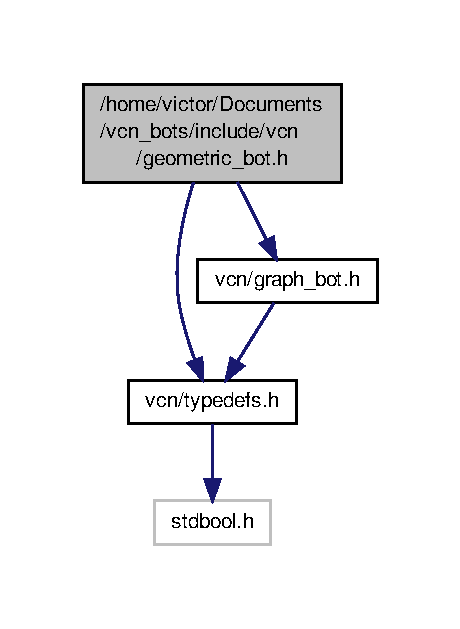
\includegraphics[width=221pt]{geometric__bot_8h__incl}
\end{center}
\end{figure}
This graph shows which files directly or indirectly include this file\+:
\nopagebreak
\begin{figure}[H]
\begin{center}
\leavevmode
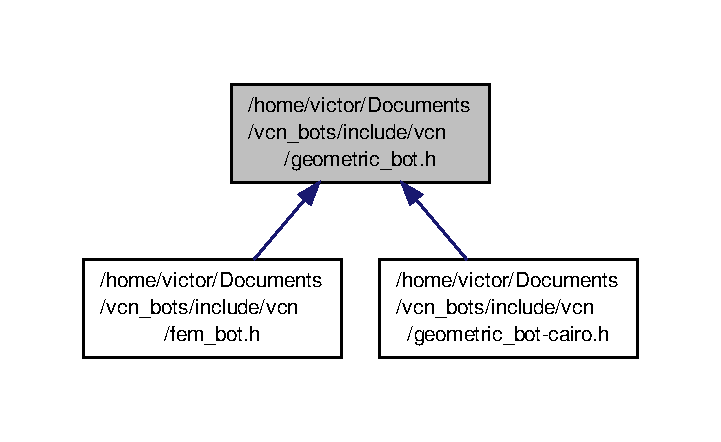
\includegraphics[width=346pt]{geometric__bot_8h__dep__incl}
\end{center}
\end{figure}
\subsection*{Classes}
\begin{DoxyCompactItemize}
\item 
struct \hyperlink{structvcn__msh3trg__s}{vcn\+\_\+msh3trg\+\_\+s}
\begin{DoxyCompactList}\small\item\em Read-\/only mesh structure, which stores the same mesh than vcn\+\_\+mesh\+\_\+t (a Delaunay triangulation), but stored in easy-\/to-\/read data structures. \end{DoxyCompactList}\item 
struct \hyperlink{structvcn__mshpoly__s}{vcn\+\_\+mshpoly\+\_\+s}
\begin{DoxyCompactList}\small\item\em Read-\/only mesh structure storing the Voronoi graph, which is a dual tesselation of the Delaunay triangulation. The Voronoi graph is a mesh conformed by convex polygons, with the property that the closest centroid of any point in the graph is the centroid of the polygon where such a point is located. \end{DoxyCompactList}\item 
struct \hyperlink{structvcn__mshpack__s}{vcn\+\_\+mshpack\+\_\+s}
\begin{DoxyCompactList}\small\item\em Read-\/only mesh structure, which stores a 2\+D sphere packing produced from the triangulation in vcn\+\_\+mesh\+\_\+t. \end{DoxyCompactList}\end{DoxyCompactItemize}
\subsection*{Macros}
\begin{DoxyCompactItemize}
\item 
\hypertarget{geometric__bot_8h_a6051d96ebad27c49f9692183a104fd19}{\#define \hyperlink{geometric__bot_8h_a6051d96ebad27c49f9692183a104fd19}{V\+C\+N\+\_\+\+A\+N\+G\+L\+E\+\_\+\+U\+N\+C}~(0.\+0)}\label{geometric__bot_8h_a6051d96ebad27c49f9692183a104fd19}

\begin{DoxyCompactList}\small\item\em Set as max\+\_\+angle param in \hyperlink{geometric__bot_8h_a65fe7a5b5494e394f0ad7c3ae0fa0165}{vcn\+\_\+mesh\+\_\+refine()} for unconstrained minimum angle. \end{DoxyCompactList}\item 
\hypertarget{geometric__bot_8h_a795ccb25076ecff6345045242d7a1cb3}{\#define \hyperlink{geometric__bot_8h_a795ccb25076ecff6345045242d7a1cb3}{V\+C\+N\+\_\+\+A\+N\+G\+L\+E\+\_\+\+M\+A\+X}~(0.\+46163958715250017309)}\label{geometric__bot_8h_a795ccb25076ecff6345045242d7a1cb3}

\begin{DoxyCompactList}\small\item\em Set as max\+\_\+angle param in \hyperlink{geometric__bot_8h_a65fe7a5b5494e394f0ad7c3ae0fa0165}{vcn\+\_\+mesh\+\_\+refine()} in order to generate a refined mesh with the maximum quality predicted by theory. Minimum angle bound equivalent to 26.\+45 degrees. \end{DoxyCompactList}\item 
\hypertarget{geometric__bot_8h_aec8e05d177222d7f57eb18979d73a3f3}{\#define \hyperlink{geometric__bot_8h_aec8e05d177222d7f57eb18979d73a3f3}{V\+C\+N\+\_\+\+D\+E\+N\+S\+I\+T\+Y\+\_\+\+C\+D\+T}~((void$\ast$)1)}\label{geometric__bot_8h_aec8e05d177222d7f57eb18979d73a3f3}

\begin{DoxyCompactList}\small\item\em Set as density function in \hyperlink{geometric__bot_8h_a65fe7a5b5494e394f0ad7c3ae0fa0165}{vcn\+\_\+mesh\+\_\+refine()} to create the Constrained Delaunay Triangulation of the domain, without inserting new vertices. \end{DoxyCompactList}\item 
\hypertarget{geometric__bot_8h_ae9aa8758a412fda9ccc6136ffbaaa791}{\#define \hyperlink{geometric__bot_8h_ae9aa8758a412fda9ccc6136ffbaaa791}{V\+C\+N\+\_\+\+D\+E\+N\+S\+I\+T\+Y\+\_\+\+M\+A\+X}~((void$\ast$)2)}\label{geometric__bot_8h_ae9aa8758a412fda9ccc6136ffbaaa791}

\begin{DoxyCompactList}\small\item\em Set as density function in \hyperlink{geometric__bot_8h_a65fe7a5b5494e394f0ad7c3ae0fa0165}{vcn\+\_\+mesh\+\_\+refine()} to create a mesh by defining the max size of edges in the output. \end{DoxyCompactList}\item 
\hypertarget{geometric__bot_8h_afeaa07a01d3c9649a1f7401d4ecee362}{\#define \hyperlink{geometric__bot_8h_afeaa07a01d3c9649a1f7401d4ecee362}{V\+C\+N\+\_\+\+D\+E\+N\+S\+I\+T\+Y\+\_\+\+I\+M\+G}~((void$\ast$)3)}\label{geometric__bot_8h_afeaa07a01d3c9649a1f7401d4ecee362}

\begin{DoxyCompactList}\small\item\em Set as density function in \hyperlink{geometric__bot_8h_a65fe7a5b5494e394f0ad7c3ae0fa0165}{vcn\+\_\+mesh\+\_\+refine()} to utilize an image as density function. \end{DoxyCompactList}\item 
\hypertarget{geometric__bot_8h_a6ec080f4e38bb40ceac0e04a99dadeaf}{\#define \hyperlink{geometric__bot_8h_a6ec080f4e38bb40ceac0e04a99dadeaf}{V\+C\+N\+\_\+\+L\+A\+B\+E\+L\+I\+N\+G\+\_\+\+A\+M\+D}~((void$\ast$)1)}\label{geometric__bot_8h_a6ec080f4e38bb40ceac0e04a99dadeaf}

\begin{DoxyCompactList}\small\item\em Set as labeling function in \hyperlink{geometric__bot_8h_a0952856f723e71f6461e84910f506214}{vcn\+\_\+mesh\+\_\+get\+\_\+msh3trg()} to ennumerate the nodes by reducing the fill-\/in of the L\+U decomposition of the adjacency matrix. Using the Approximate Minimum Degree algorithm. \end{DoxyCompactList}\end{DoxyCompactItemize}
\subsection*{Typedefs}
\begin{DoxyCompactItemize}
\item 
\hypertarget{geometric__bot_8h_a10375cbf3125046dc59bd4bef92432ad}{typedef struct vcn\+\_\+model\+\_\+s \hyperlink{geometric__bot_8h_a10375cbf3125046dc59bd4bef92432ad}{vcn\+\_\+model\+\_\+t}}\label{geometric__bot_8h_a10375cbf3125046dc59bd4bef92432ad}

\begin{DoxyCompactList}\small\item\em Geometry model defining the domain. \end{DoxyCompactList}\item 
\hypertarget{geometric__bot_8h_a8942da13867aa76dd55d8f2b079ad3ce}{typedef struct vcn\+\_\+mesh\+\_\+s \hyperlink{geometric__bot_8h_a8942da13867aa76dd55d8f2b079ad3ce}{vcn\+\_\+mesh\+\_\+t}}\label{geometric__bot_8h_a8942da13867aa76dd55d8f2b079ad3ce}

\begin{DoxyCompactList}\small\item\em Write-\/only mesh structure used to create and modify meshes. This mesh is based on a Delaunay triangulation. In order to read the mesh, it must be \char`\"{}converted\char`\"{} into a read-\/only structure, such as vcn\+\_\+msh3trg\+\_\+t. \end{DoxyCompactList}\item 
\hypertarget{geometric__bot_8h_af753a8fb5e30b4d81a02489e92b54df2}{typedef struct \hyperlink{structvcn__msh3trg__s}{vcn\+\_\+msh3trg\+\_\+s} \hyperlink{geometric__bot_8h_af753a8fb5e30b4d81a02489e92b54df2}{vcn\+\_\+msh3trg\+\_\+t}}\label{geometric__bot_8h_af753a8fb5e30b4d81a02489e92b54df2}

\begin{DoxyCompactList}\small\item\em Read-\/only mesh structure, which stores the same mesh than vcn\+\_\+mesh\+\_\+t (a Delaunay triangulation), but stored in easy-\/to-\/read data structures. \end{DoxyCompactList}\item 
\hypertarget{geometric__bot_8h_a25e055df6f6e0902c79e1f37ef4cc329}{typedef struct \hyperlink{structvcn__mshpoly__s}{vcn\+\_\+mshpoly\+\_\+s} \hyperlink{geometric__bot_8h_a25e055df6f6e0902c79e1f37ef4cc329}{vcn\+\_\+mshpoly\+\_\+t}}\label{geometric__bot_8h_a25e055df6f6e0902c79e1f37ef4cc329}

\begin{DoxyCompactList}\small\item\em Read-\/only mesh structure storing the Voronoi graph, which is a dual tesselation of the Delaunay triangulation. The Voronoi graph is a mesh conformed by convex polygons, with the property that the closest centroid of any point in the graph is the centroid of the polygon where such a point is located. \end{DoxyCompactList}\item 
\hypertarget{geometric__bot_8h_aa1e47f3fc55677e96c43ca151d971d86}{typedef struct \hyperlink{structvcn__mshpack__s}{vcn\+\_\+mshpack\+\_\+s} \hyperlink{geometric__bot_8h_aa1e47f3fc55677e96c43ca151d971d86}{vcn\+\_\+mshpack\+\_\+t}}\label{geometric__bot_8h_aa1e47f3fc55677e96c43ca151d971d86}

\begin{DoxyCompactList}\small\item\em Read-\/only mesh structure, which stores a 2\+D sphere packing produced from the triangulation in vcn\+\_\+mesh\+\_\+t. \end{DoxyCompactList}\item 
\hypertarget{geometric__bot_8h_ae4c41c6290ca2bb2c68749b5d6aaa93e}{typedef struct vcn\+\_\+density\+\_\+img\+\_\+s \hyperlink{geometric__bot_8h_ae4c41c6290ca2bb2c68749b5d6aaa93e}{vcn\+\_\+density\+\_\+img\+\_\+t}}\label{geometric__bot_8h_ae4c41c6290ca2bb2c68749b5d6aaa93e}

\begin{DoxyCompactList}\small\item\em Built-\/in image used to calculate the density of a given point. \end{DoxyCompactList}\end{DoxyCompactItemize}
\subsection*{Functions}
\begin{DoxyCompactItemize}
\item 
\hyperlink{geometric__bot_8h_a10375cbf3125046dc59bd4bef92432ad}{vcn\+\_\+model\+\_\+t} $\ast$ \hyperlink{geometric__bot_8h_a1a446c6b4539efa1d38d3d7413747627}{vcn\+\_\+model\+\_\+load} (const char $\ast$filename)
\begin{DoxyCompactList}\small\item\em Load geometry from a plain text file. \end{DoxyCompactList}\item 
\hyperlink{geometric__bot_8h_a10375cbf3125046dc59bd4bef92432ad}{vcn\+\_\+model\+\_\+t} $\ast$ \hyperlink{geometric__bot_8h_a161dcc3f517ff5ca53ffac145ab40f35}{vcn\+\_\+model\+\_\+create} (double $\ast$vertices, uint N\+\_\+vertices, uint $\ast$segments, uint N\+\_\+segments, double $\ast$holes, uint N\+\_\+holes)
\begin{DoxyCompactList}\small\item\em Create model from input data. \end{DoxyCompactList}\item 
\hyperlink{geometric__bot_8h_a10375cbf3125046dc59bd4bef92432ad}{vcn\+\_\+model\+\_\+t} $\ast$ \hyperlink{geometric__bot_8h_a5aac5fee89c01765e39eda2201d401cc}{vcn\+\_\+model\+\_\+create\+\_\+rectangle} (double x\+\_\+min, double y\+\_\+min, double x\+\_\+max, double y\+\_\+max)
\begin{DoxyCompactList}\small\item\em Creates a geometry model of a rectangle. \end{DoxyCompactList}\item 
\hyperlink{geometric__bot_8h_a10375cbf3125046dc59bd4bef92432ad}{vcn\+\_\+model\+\_\+t} $\ast$ \hyperlink{geometric__bot_8h_a04f48b97e88e777faa8fce535c2b2d19}{vcn\+\_\+model\+\_\+create\+\_\+polygon} (double radius, double x\+\_\+center, double y\+\_\+center, uint N\+\_\+sides)
\begin{DoxyCompactList}\small\item\em Creates a geometry model of a regular polygon. \end{DoxyCompactList}\item 
\hyperlink{geometric__bot_8h_a10375cbf3125046dc59bd4bef92432ad}{vcn\+\_\+model\+\_\+t} $\ast$ \hyperlink{geometric__bot_8h_a2ec53fd8e54d45f57fa9f745a6cb8eeb}{vcn\+\_\+model\+\_\+create\+\_\+from\+\_\+msh3trg} (const \hyperlink{geometric__bot_8h_af753a8fb5e30b4d81a02489e92b54df2}{vcn\+\_\+msh3trg\+\_\+t} $\ast$const msh3trg)
\begin{DoxyCompactList}\small\item\em Build a geometry model from a triangulation. \end{DoxyCompactList}\item 
\hyperlink{geometric__bot_8h_a10375cbf3125046dc59bd4bef92432ad}{vcn\+\_\+model\+\_\+t} $\ast$ \hyperlink{geometric__bot_8h_a1fdf604dc0fe2213068d9c72360db5c6}{vcn\+\_\+model\+\_\+create\+\_\+from\+\_\+msh3trg\+\_\+with\+\_\+disabled\+\_\+trg} (const \hyperlink{geometric__bot_8h_af753a8fb5e30b4d81a02489e92b54df2}{vcn\+\_\+msh3trg\+\_\+t} $\ast$const msh3trg, const bool $\ast$const trg\+\_\+enabled, uint $\ast$N\+\_\+real\+\_\+vtx\+\_\+boundaries, uint $\ast$$\ast$real\+\_\+vtx\+\_\+boundaries)
\begin{DoxyCompactList}\small\item\em Build a geometry model from a triangulation with disabled triangles. \end{DoxyCompactList}\item 
void \hyperlink{geometric__bot_8h_a0043072f854544633f10ba9428fdce3a}{vcn\+\_\+model\+\_\+set\+\_\+enveloped\+\_\+areas\+\_\+as\+\_\+holes} (\hyperlink{geometric__bot_8h_a10375cbf3125046dc59bd4bef92432ad}{vcn\+\_\+model\+\_\+t} $\ast$model)
\begin{DoxyCompactList}\small\item\em Mark as holes all the enveloped areas in the model. The enveloped areas are internal bounded areas. \end{DoxyCompactList}\item 
\hyperlink{geometric__bot_8h_a10375cbf3125046dc59bd4bef92432ad}{vcn\+\_\+model\+\_\+t} $\ast$ \hyperlink{geometric__bot_8h_ac390733b18a46bc5171a86ec8e69e43c}{vcn\+\_\+model\+\_\+clone} (const \hyperlink{geometric__bot_8h_a10375cbf3125046dc59bd4bef92432ad}{vcn\+\_\+model\+\_\+t} $\ast$const model)
\begin{DoxyCompactList}\small\item\em Create an identical copy of the model. \end{DoxyCompactList}\item 
\hypertarget{geometric__bot_8h_a18b4a66a322d4b6a3739399c918c9b0f}{\hyperlink{graph__bot_8h_a3a951da0c05a3e2ab67d73a94269fdab}{vcn\+\_\+graph\+\_\+t} $\ast$ {\bfseries vcn\+\_\+model\+\_\+get\+\_\+vtx\+\_\+graph} (const \hyperlink{geometric__bot_8h_a10375cbf3125046dc59bd4bef92432ad}{vcn\+\_\+model\+\_\+t} $\ast$const model)}\label{geometric__bot_8h_a18b4a66a322d4b6a3739399c918c9b0f}

\item 
bool \hyperlink{geometric__bot_8h_aadc25ee97bb3ea0f61a8302f1723d81a}{vcn\+\_\+model\+\_\+is\+\_\+vtx\+\_\+inside} (const \hyperlink{geometric__bot_8h_a10375cbf3125046dc59bd4bef92432ad}{vcn\+\_\+model\+\_\+t} $\ast$const model, const double $\ast$const vtx)
\begin{DoxyCompactList}\small\item\em Check if the vertex lies inside the model. ~\newline
{\bfseries W\+A\+R\+N\+I\+N\+G\+:} A mesh is built internally, making this function expensive, if you are going to test several vertices for the same model please build a mesh using V\+C\+N\+\_\+\+D\+E\+N\+S\+I\+T\+Y\+\_\+\+C\+D\+T and use the function \hyperlink{geometric__bot_8h_a9c414c9576b316c022d1dd6847f701e4}{vcn\+\_\+mesh\+\_\+is\+\_\+vtx\+\_\+inside()}. \end{DoxyCompactList}\item 
void \hyperlink{geometric__bot_8h_accc7820ad1c8fee93b13be48f292ac10}{vcn\+\_\+model\+\_\+export\+\_\+to\+\_\+asymptote} (const \hyperlink{geometric__bot_8h_a10375cbf3125046dc59bd4bef92432ad}{vcn\+\_\+model\+\_\+t} $\ast$const model, const char $\ast$filename)
\begin{DoxyCompactList}\small\item\em Export the \href{http://asymptote.sourceforge.net/}{\tt Asymptote} code to generate an image of the model. \end{DoxyCompactList}\item 
void \hyperlink{geometric__bot_8h_a7082312493d6b8d46a75b525177479b7}{vcn\+\_\+model\+\_\+destroy} (\hyperlink{geometric__bot_8h_a10375cbf3125046dc59bd4bef92432ad}{vcn\+\_\+model\+\_\+t} $\ast$model)
\begin{DoxyCompactList}\small\item\em Destroy the model. \end{DoxyCompactList}\item 
uchar \hyperlink{geometric__bot_8h_a148e58df14b39c8a8d29cf2ba5061e83}{vcn\+\_\+model\+\_\+save} (const \hyperlink{geometric__bot_8h_a10375cbf3125046dc59bd4bef92432ad}{vcn\+\_\+model\+\_\+t} $\ast$const model, const char $\ast$filename)
\begin{DoxyCompactList}\small\item\em Save model into a plain text file. \end{DoxyCompactList}\item 
int \hyperlink{geometric__bot_8h_aff5e6a9d38c001491a171b165e5aa42b}{vcn\+\_\+model\+\_\+verify\+\_\+consistence} (const \hyperlink{geometric__bot_8h_a10375cbf3125046dc59bd4bef92432ad}{vcn\+\_\+model\+\_\+t} $\ast$const model, uint ids\+\_\+causing\+\_\+error\mbox{[}2\mbox{]})
\item 
void \hyperlink{geometric__bot_8h_a824bd2ac57d111a80f5406815c716a2e}{vcn\+\_\+model\+\_\+get\+\_\+enveloping\+\_\+box} (const \hyperlink{geometric__bot_8h_a10375cbf3125046dc59bd4bef92432ad}{vcn\+\_\+model\+\_\+t} $\ast$const model, double box\mbox{[}4\mbox{]})
\begin{DoxyCompactList}\small\item\em Get enveloping box of the model. \end{DoxyCompactList}\item 
\hypertarget{geometric__bot_8h_a2a5f5539a3888a145349457da17cf45f}{int {\bfseries vcn\+\_\+model\+\_\+regularize} (\hyperlink{geometric__bot_8h_a10375cbf3125046dc59bd4bef92432ad}{vcn\+\_\+model\+\_\+t} $\ast$model, double lambda, uint N\+\_\+fixed\+\_\+vertices, uint $\ast$fixed\+\_\+vertices)}\label{geometric__bot_8h_a2a5f5539a3888a145349457da17cf45f}

\item 
\hypertarget{geometric__bot_8h_ae662046c5a369fbbacde498bf0eaa5ed}{void {\bfseries vcn\+\_\+model\+\_\+collapse\+\_\+small\+\_\+segments} (\hyperlink{geometric__bot_8h_a10375cbf3125046dc59bd4bef92432ad}{vcn\+\_\+model\+\_\+t} $\ast$model, double tolerance, uint N\+\_\+fixed\+\_\+vertices, uint $\ast$fixed\+\_\+vertices)}\label{geometric__bot_8h_ae662046c5a369fbbacde498bf0eaa5ed}

\item 
\hypertarget{geometric__bot_8h_a42f4dffda1440e370dd529bd3c945b1d}{void {\bfseries vcn\+\_\+model\+\_\+collapse\+\_\+colinear\+\_\+vertices} (\hyperlink{geometric__bot_8h_a10375cbf3125046dc59bd4bef92432ad}{vcn\+\_\+model\+\_\+t} $\ast$model, uint N\+\_\+fixed\+\_\+vertices, uint $\ast$fixed\+\_\+vertices, double tolerance)}\label{geometric__bot_8h_a42f4dffda1440e370dd529bd3c945b1d}

\item 
\hypertarget{geometric__bot_8h_a4afe06c5f25b2b770c455a496933e3c2}{\hyperlink{geometric__bot_8h_a10375cbf3125046dc59bd4bef92432ad}{vcn\+\_\+model\+\_\+t} $\ast$ {\bfseries vcn\+\_\+model\+\_\+get\+\_\+combination} (const \hyperlink{geometric__bot_8h_a10375cbf3125046dc59bd4bef92432ad}{vcn\+\_\+model\+\_\+t} $\ast$const model1, const \hyperlink{geometric__bot_8h_a10375cbf3125046dc59bd4bef92432ad}{vcn\+\_\+model\+\_\+t} $\ast$const model2, double min\+\_\+length\+\_\+x\+\_\+segment)}\label{geometric__bot_8h_a4afe06c5f25b2b770c455a496933e3c2}

\item 
\hypertarget{geometric__bot_8h_a9f55828a4e3852357ac27b9faa67ccd3}{\hyperlink{geometric__bot_8h_a10375cbf3125046dc59bd4bef92432ad}{vcn\+\_\+model\+\_\+t} $\ast$ {\bfseries vcn\+\_\+model\+\_\+get\+\_\+intersection} (const \hyperlink{geometric__bot_8h_a10375cbf3125046dc59bd4bef92432ad}{vcn\+\_\+model\+\_\+t} $\ast$const model1, const \hyperlink{geometric__bot_8h_a10375cbf3125046dc59bd4bef92432ad}{vcn\+\_\+model\+\_\+t} $\ast$const model2, double min\+\_\+length\+\_\+x\+\_\+segment)}\label{geometric__bot_8h_a9f55828a4e3852357ac27b9faa67ccd3}

\item 
\hypertarget{geometric__bot_8h_af0047583497a34e7af27b2ad778a3d4c}{\hyperlink{geometric__bot_8h_a10375cbf3125046dc59bd4bef92432ad}{vcn\+\_\+model\+\_\+t} $\ast$ {\bfseries vcn\+\_\+model\+\_\+get\+\_\+union} (const \hyperlink{geometric__bot_8h_a10375cbf3125046dc59bd4bef92432ad}{vcn\+\_\+model\+\_\+t} $\ast$const model1, const \hyperlink{geometric__bot_8h_a10375cbf3125046dc59bd4bef92432ad}{vcn\+\_\+model\+\_\+t} $\ast$const model2, double min\+\_\+length\+\_\+x\+\_\+segment)}\label{geometric__bot_8h_af0047583497a34e7af27b2ad778a3d4c}

\item 
\hypertarget{geometric__bot_8h_a869dffb6e0a2abb61cb1df612769020f}{double $\ast$ {\bfseries vcn\+\_\+model\+\_\+get\+\_\+holes} (const \hyperlink{geometric__bot_8h_a10375cbf3125046dc59bd4bef92432ad}{vcn\+\_\+model\+\_\+t} $\ast$const model, uint $\ast$N\+\_\+holes)}\label{geometric__bot_8h_a869dffb6e0a2abb61cb1df612769020f}

\item 
\hypertarget{geometric__bot_8h_a205c9a0e07b909077efd7a8d220a065a}{double $\ast$ {\bfseries vcn\+\_\+model\+\_\+get\+\_\+vertices} (const \hyperlink{geometric__bot_8h_a10375cbf3125046dc59bd4bef92432ad}{vcn\+\_\+model\+\_\+t} $\ast$const model, uint $\ast$N\+\_\+vertices)}\label{geometric__bot_8h_a205c9a0e07b909077efd7a8d220a065a}

\item 
\hypertarget{geometric__bot_8h_af3113e923478b2690f22d41a7c86a0e2}{void {\bfseries vcn\+\_\+model\+\_\+unify\+\_\+edge} (\hyperlink{geometric__bot_8h_a10375cbf3125046dc59bd4bef92432ad}{vcn\+\_\+model\+\_\+t} $\ast$model, double $\ast$vtx1, double $\ast$vtx2)}\label{geometric__bot_8h_af3113e923478b2690f22d41a7c86a0e2}

\item 
\hypertarget{geometric__bot_8h_a29213475e1b4372ba08978c73e597f8c}{uint {\bfseries vcn\+\_\+model\+\_\+get\+\_\+vertex\+\_\+id} (const \hyperlink{geometric__bot_8h_a10375cbf3125046dc59bd4bef92432ad}{vcn\+\_\+model\+\_\+t} $\ast$const model, double $\ast$vtx)}\label{geometric__bot_8h_a29213475e1b4372ba08978c73e597f8c}

\item 
\hypertarget{geometric__bot_8h_a041d025b8d7aa16c9f4b3b6f9607c3d3}{double $\ast$ {\bfseries vcn\+\_\+model\+\_\+get\+\_\+vertex\+\_\+coordinate} (const \hyperlink{geometric__bot_8h_a10375cbf3125046dc59bd4bef92432ad}{vcn\+\_\+model\+\_\+t} $\ast$const model, uint id)}\label{geometric__bot_8h_a041d025b8d7aa16c9f4b3b6f9607c3d3}

\item 
\hypertarget{geometric__bot_8h_a4f3e130eba4f49d84a57b8fe4176fc67}{uint {\bfseries vcn\+\_\+model\+\_\+get\+\_\+edge\+\_\+id} (const \hyperlink{geometric__bot_8h_a10375cbf3125046dc59bd4bef92432ad}{vcn\+\_\+model\+\_\+t} $\ast$const model, double $\ast$edge\+\_\+vertices)}\label{geometric__bot_8h_a4f3e130eba4f49d84a57b8fe4176fc67}

\item 
\hypertarget{geometric__bot_8h_a58ce32bfc1373d05e77da9e0e7fcc163}{double $\ast$ {\bfseries vcn\+\_\+model\+\_\+get\+\_\+edge\+\_\+coordinates} (const \hyperlink{geometric__bot_8h_a10375cbf3125046dc59bd4bef92432ad}{vcn\+\_\+model\+\_\+t} $\ast$const model, uint id)}\label{geometric__bot_8h_a58ce32bfc1373d05e77da9e0e7fcc163}

\item 
\hypertarget{geometric__bot_8h_adccb4756e7ace7a8699ee27458fb0590}{uint {\bfseries vcn\+\_\+model\+\_\+get\+\_\+number\+\_\+of\+\_\+vertices} (const \hyperlink{geometric__bot_8h_a10375cbf3125046dc59bd4bef92432ad}{vcn\+\_\+model\+\_\+t} $\ast$const model)}\label{geometric__bot_8h_adccb4756e7ace7a8699ee27458fb0590}

\item 
\hypertarget{geometric__bot_8h_a05f48a63d8ff358b49f1ca370358b832}{uint {\bfseries vcn\+\_\+model\+\_\+get\+\_\+number\+\_\+of\+\_\+edges} (const \hyperlink{geometric__bot_8h_a10375cbf3125046dc59bd4bef92432ad}{vcn\+\_\+model\+\_\+t} $\ast$const model)}\label{geometric__bot_8h_a05f48a63d8ff358b49f1ca370358b832}

\item 
\hypertarget{geometric__bot_8h_ac4ed1574eefbd3a93b6c8632d4318ab2}{uint {\bfseries vcn\+\_\+model\+\_\+get\+\_\+number\+\_\+of\+\_\+hole\+\_\+seeds} (const \hyperlink{geometric__bot_8h_a10375cbf3125046dc59bd4bef92432ad}{vcn\+\_\+model\+\_\+t} $\ast$const model)}\label{geometric__bot_8h_ac4ed1574eefbd3a93b6c8632d4318ab2}

\item 
\hypertarget{geometric__bot_8h_aae89c4a4c3493179496bf7af691ac832}{double {\bfseries vcn\+\_\+model\+\_\+get\+\_\+length\+\_\+of\+\_\+ith\+\_\+edge} (const \hyperlink{geometric__bot_8h_a10375cbf3125046dc59bd4bef92432ad}{vcn\+\_\+model\+\_\+t} $\ast$model, uint i)}\label{geometric__bot_8h_aae89c4a4c3493179496bf7af691ac832}

\item 
\hypertarget{geometric__bot_8h_afd8108c91cb8eac0fe0b8c10f6a643b6}{double {\bfseries vcn\+\_\+model\+\_\+get\+\_\+area} (const \hyperlink{geometric__bot_8h_a10375cbf3125046dc59bd4bef92432ad}{vcn\+\_\+model\+\_\+t} $\ast$const model)}\label{geometric__bot_8h_afd8108c91cb8eac0fe0b8c10f6a643b6}

\item 
\hypertarget{geometric__bot_8h_a3d6fa1f39cb7d4e4ef0d74f9e40a8c70}{double {\bfseries vcn\+\_\+model\+\_\+get\+\_\+sum\+\_\+of\+\_\+sgm\+\_\+length} (const \hyperlink{geometric__bot_8h_a10375cbf3125046dc59bd4bef92432ad}{vcn\+\_\+model\+\_\+t} $\ast$const model)}\label{geometric__bot_8h_a3d6fa1f39cb7d4e4ef0d74f9e40a8c70}

\item 
\hyperlink{geometric__bot_8h_ae4c41c6290ca2bb2c68749b5d6aaa93e}{vcn\+\_\+density\+\_\+img\+\_\+t} $\ast$ \hyperlink{geometric__bot_8h_ae41611191433b9ff27edfc9ae04dde37}{vcn\+\_\+density\+\_\+img\+\_\+create} (const char $\ast$filename, double scale, double xdisp, double ydisp, double max\+\_\+density)
\begin{DoxyCompactList}\small\item\em Read the image to be used in the density calculation. \end{DoxyCompactList}\item 
uint \hyperlink{geometric__bot_8h_a475dd3dc6e13acc2ff91de576dff518a}{vcn\+\_\+density\+\_\+img\+\_\+get\+\_\+width} (const \hyperlink{geometric__bot_8h_ae4c41c6290ca2bb2c68749b5d6aaa93e}{vcn\+\_\+density\+\_\+img\+\_\+t} $\ast$const data)
\begin{DoxyCompactList}\small\item\em Returns the image's width. \end{DoxyCompactList}\item 
uint \hyperlink{geometric__bot_8h_a02e7af90ac66a402e9a82842664cb1dc}{vcn\+\_\+density\+\_\+img\+\_\+get\+\_\+height} (const \hyperlink{geometric__bot_8h_ae4c41c6290ca2bb2c68749b5d6aaa93e}{vcn\+\_\+density\+\_\+img\+\_\+t} $\ast$const data)
\begin{DoxyCompactList}\small\item\em Returns the image's height. \end{DoxyCompactList}\item 
void \hyperlink{geometric__bot_8h_a8ba717d871bf9b5c9592ee7ee5c7b588}{vcn\+\_\+density\+\_\+img\+\_\+destroy} (\hyperlink{geometric__bot_8h_ae4c41c6290ca2bb2c68749b5d6aaa93e}{vcn\+\_\+density\+\_\+img\+\_\+t} $\ast$data)
\begin{DoxyCompactList}\small\item\em Destroys the density image data. \end{DoxyCompactList}\item 
\hyperlink{geometric__bot_8h_a8942da13867aa76dd55d8f2b079ad3ce}{vcn\+\_\+mesh\+\_\+t} $\ast$ \hyperlink{geometric__bot_8h_a25fc194513d321be3bdd4a94c27d3709}{vcn\+\_\+mesh\+\_\+clone} (const \hyperlink{geometric__bot_8h_a8942da13867aa76dd55d8f2b079ad3ce}{vcn\+\_\+mesh\+\_\+t} $\ast$const mesh)
\begin{DoxyCompactList}\small\item\em Create an identical copy of the mesh. \end{DoxyCompactList}\item 
\hyperlink{geometric__bot_8h_a8942da13867aa76dd55d8f2b079ad3ce}{vcn\+\_\+mesh\+\_\+t} $\ast$ \hyperlink{geometric__bot_8h_a69fd725376344576722d7867ba2e38cc}{vcn\+\_\+mesh\+\_\+create\+\_\+\+Delaunay} (uint N\+\_\+vertices, const double $\ast$const vertices)
\begin{DoxyCompactList}\small\item\em Create a Delaunay triangulation from a given set of vertices. \end{DoxyCompactList}\item 
\hyperlink{geometric__bot_8h_a8942da13867aa76dd55d8f2b079ad3ce}{vcn\+\_\+mesh\+\_\+t} $\ast$ \hyperlink{geometric__bot_8h_abdaeeb97be899e58961dec2b1efd3642}{vcn\+\_\+mesh\+\_\+create\+\_\+\+C\+D\+T} (const \hyperlink{geometric__bot_8h_a10375cbf3125046dc59bd4bef92432ad}{vcn\+\_\+model\+\_\+t} $\ast$const model)
\begin{DoxyCompactList}\small\item\em Create a Constrained Delaunay triangulation from a given P\+S\+L. \end{DoxyCompactList}\item 
\hyperlink{geometric__bot_8h_a8942da13867aa76dd55d8f2b079ad3ce}{vcn\+\_\+mesh\+\_\+t} $\ast$ \hyperlink{geometric__bot_8h_a2ac4cbf143b4b43575a95c9e5dad8483}{vcn\+\_\+mesh\+\_\+create\+\_\+from\+\_\+model} (const \hyperlink{geometric__bot_8h_a10375cbf3125046dc59bd4bef92432ad}{vcn\+\_\+model\+\_\+t} $\ast$const model, uint max\+\_\+vtx, uint max\+\_\+trg, double min\+\_\+angle, double($\ast$density)(const double $\ast$const x, const void $\ast$const data), const void $\ast$const density\+\_\+data)
\begin{DoxyCompactList}\small\item\em Creates a mesh from a Planar Straight Line Graph (P\+S\+L\+G, encoded in the model) as exposed by Schewchuck\+: \end{DoxyCompactList}\item 
\hyperlink{graph__bot_8h_a3a951da0c05a3e2ab67d73a94269fdab}{vcn\+\_\+graph\+\_\+t} $\ast$ \hyperlink{geometric__bot_8h_a712d685c11cdf23a13884e42923ee926}{vcn\+\_\+mesh\+\_\+create\+\_\+vtx\+\_\+graph} (const \hyperlink{geometric__bot_8h_a8942da13867aa76dd55d8f2b079ad3ce}{vcn\+\_\+mesh\+\_\+t} $\ast$const mesh)
\begin{DoxyCompactList}\small\item\em Build a graph from the triangular mesh. Each vertex of the mesh represent a node in the graph. ~\newline
{\bfseries W\+A\+R\+N\+I\+N\+G\+:} Assuming that vertices has an I\+D as attribute. \end{DoxyCompactList}\item 
\hyperlink{graph__bot_8h_a3a951da0c05a3e2ab67d73a94269fdab}{vcn\+\_\+graph\+\_\+t} $\ast$ \hyperlink{geometric__bot_8h_a7eff21b3ddc55dab0ecda1c830f14e84}{vcn\+\_\+mesh\+\_\+create\+\_\+elem\+\_\+graph} (const \hyperlink{geometric__bot_8h_a8942da13867aa76dd55d8f2b079ad3ce}{vcn\+\_\+mesh\+\_\+t} $\ast$const mesh)
\begin{DoxyCompactList}\small\item\em Build a graph from the triangular mesh. Each element of the mesh represent a node in the graph. ~\newline
{\bfseries W\+A\+R\+N\+I\+N\+G\+:} Assuming that triangles has an I\+D as attribute. \end{DoxyCompactList}\item 
void \hyperlink{geometric__bot_8h_a71f17341ecfa0a0a85194e83ac99093b}{vcn\+\_\+mesh\+\_\+duplicate\+\_\+one\+\_\+point\+\_\+connections} (\hyperlink{geometric__bot_8h_a8942da13867aa76dd55d8f2b079ad3ce}{vcn\+\_\+mesh\+\_\+t} $\ast$mesh)
\begin{DoxyCompactList}\small\item\em Duplicate vertices which are the only intersection of two disjoint portions of the mesh in order to disconnect such portions. \end{DoxyCompactList}\item 
void \hyperlink{geometric__bot_8h_ac3a85ac5cae0601e24c0bacff46dd666}{vcn\+\_\+mesh\+\_\+destroy} (\hyperlink{geometric__bot_8h_a8942da13867aa76dd55d8f2b079ad3ce}{vcn\+\_\+mesh\+\_\+t} $\ast$mesh)
\begin{DoxyCompactList}\small\item\em Destroy mesh. \end{DoxyCompactList}\item 
bool \hyperlink{geometric__bot_8h_a9c414c9576b316c022d1dd6847f701e4}{vcn\+\_\+mesh\+\_\+is\+\_\+vtx\+\_\+inside} (const \hyperlink{geometric__bot_8h_a8942da13867aa76dd55d8f2b079ad3ce}{vcn\+\_\+mesh\+\_\+t} $\ast$const mesh, const double $\ast$const vtx)
\begin{DoxyCompactList}\small\item\em Check if the vertex lies inside the mesh. \end{DoxyCompactList}\item 
void \hyperlink{geometric__bot_8h_a65fe7a5b5494e394f0ad7c3ae0fa0165}{vcn\+\_\+mesh\+\_\+refine} (\hyperlink{geometric__bot_8h_a8942da13867aa76dd55d8f2b079ad3ce}{vcn\+\_\+mesh\+\_\+t} $\ast$const mesh, uint max\+\_\+vtx, uint max\+\_\+trg, double min\+\_\+angle, double($\ast$density)(const double $\ast$const x, const void $\ast$const data), const void $\ast$const density\+\_\+data)
\begin{DoxyCompactList}\small\item\em Produces a refined Delaunay triangulation. The algorithm have the folowing properties\+: \end{DoxyCompactList}\item 
int \hyperlink{geometric__bot_8h_ab1172a13fc246a12f213602dd69b9c05}{vcn\+\_\+mesh\+\_\+insert\+\_\+vertex} (\hyperlink{geometric__bot_8h_a8942da13867aa76dd55d8f2b079ad3ce}{vcn\+\_\+mesh\+\_\+t} $\ast$const mesh, const double $\ast$const vertex)
\begin{DoxyCompactList}\small\item\em Insert a new vertex inside the mesh while maintaining the Delaunay condition. \end{DoxyCompactList}\item 
double $\ast$ \hyperlink{geometric__bot_8h_a7d78c4f14200632cc1f8382d81d46909}{vcn\+\_\+mesh\+\_\+get\+\_\+centroids\+\_\+of\+\_\+subareas} (const \hyperlink{geometric__bot_8h_a8942da13867aa76dd55d8f2b079ad3ce}{vcn\+\_\+mesh\+\_\+t} $\ast$const mesh, uint $\ast$N\+\_\+centroids)
\begin{DoxyCompactList}\small\item\em Calculates the pseudo-\/centroid of the sub-\/areas in the mesh. A sub-\/area is a portion of the domain which is bounded by input segments, A single mesh could have multiple subareas. The pseudo-\/centroid is the centroid of a triangle (inside the sub-\/area) which is closest to the real centroid of the whole subarea. The pseudo-\/centroid is guaranteed to be inside a concave polygon, such as most of the sub-\/areas. \end{DoxyCompactList}\item 
double $\ast$ \hyperlink{geometric__bot_8h_a3089fdf87b2d7ef499ce4b784aaa83d3}{vcn\+\_\+mesh\+\_\+get\+\_\+centroids\+\_\+of\+\_\+enveloped\+\_\+areas} (const \hyperlink{geometric__bot_8h_a8942da13867aa76dd55d8f2b079ad3ce}{vcn\+\_\+mesh\+\_\+t} $\ast$const mesh, uint $\ast$N\+\_\+centroids)
\begin{DoxyCompactList}\small\item\em A hole can be seen as an enveloped sub-\/area, which is a sub-\/area inside another enveloping subarea. This routine calculates the location of the pseudo-\/centroids of enveloped areas, which could be used to plant holes. \end{DoxyCompactList}\item 
double \hyperlink{geometric__bot_8h_aa83ac07b19d502e68d81b66a59c00db8}{vcn\+\_\+mesh\+\_\+clear\+\_\+enveloped\+\_\+areas} (\hyperlink{geometric__bot_8h_a8942da13867aa76dd55d8f2b079ad3ce}{vcn\+\_\+mesh\+\_\+t} $\ast$mesh, double $\ast$area\+\_\+removed)
\begin{DoxyCompactList}\small\item\em Delete the triangles inside enveloped areas. \end{DoxyCompactList}\item 
double \hyperlink{geometric__bot_8h_aa2643dbbe2d8d73f65793b46663e2d8a}{vcn\+\_\+mesh\+\_\+keep\+\_\+biggest\+\_\+isolated\+\_\+area} (\hyperlink{geometric__bot_8h_a8942da13867aa76dd55d8f2b079ad3ce}{vcn\+\_\+mesh\+\_\+t} $\ast$mesh, double $\ast$area\+\_\+removed)
\begin{DoxyCompactList}\small\item\em If the mesh is not a continuous domain, this function keep the biggest sub-\/area and delete the other ones. ~\newline
{\bfseries W\+A\+R\+N\+I\+N\+G}\+: After this functions is used, some input segments and input vertices will be disconnected. \end{DoxyCompactList}\item 
uint \hyperlink{geometric__bot_8h_a8dcfaf6f3afe6401566b4ad50dcefe82}{vcn\+\_\+mesh\+\_\+delete\+\_\+isolated\+\_\+segments} (\hyperlink{geometric__bot_8h_a8942da13867aa76dd55d8f2b079ad3ce}{vcn\+\_\+mesh\+\_\+t} $\ast$const mesh)
\begin{DoxyCompactList}\small\item\em Delete those input segments without adjacent triangles, which could arise if the P\+S\+L\+G is not well defined or if one of the following functions has been used\+: \hyperlink{geometric__bot_8h_aa83ac07b19d502e68d81b66a59c00db8}{vcn\+\_\+mesh\+\_\+clear\+\_\+enveloped\+\_\+areas()} or \hyperlink{geometric__bot_8h_aa2643dbbe2d8d73f65793b46663e2d8a}{vcn\+\_\+mesh\+\_\+keep\+\_\+biggest\+\_\+isolated\+\_\+area()}. \end{DoxyCompactList}\item 
uint \hyperlink{geometric__bot_8h_ac83047be991f1c92658a6df0696a46ad}{vcn\+\_\+mesh\+\_\+delete\+\_\+internal\+\_\+input\+\_\+segments} (\hyperlink{geometric__bot_8h_a8942da13867aa76dd55d8f2b079ad3ce}{vcn\+\_\+mesh\+\_\+t} $\ast$const mesh)
\begin{DoxyCompactList}\small\item\em Delete those input segments inside the boundaries. \end{DoxyCompactList}\item 
uint \hyperlink{geometric__bot_8h_a6be2b16eff83e05fd0b194e3806efdd9}{vcn\+\_\+mesh\+\_\+delete\+\_\+isolated\+\_\+vertices} (\hyperlink{geometric__bot_8h_a8942da13867aa76dd55d8f2b079ad3ce}{vcn\+\_\+mesh\+\_\+t} $\ast$mesh)
\begin{DoxyCompactList}\small\item\em Delete those input vertices disconnected from the mesh, which could arise if the P\+S\+L\+G is not well defined or if the function \hyperlink{geometric__bot_8h_a8dcfaf6f3afe6401566b4ad50dcefe82}{vcn\+\_\+mesh\+\_\+delete\+\_\+isolated\+\_\+segments()} has been used. \end{DoxyCompactList}\item 
\hypertarget{geometric__bot_8h_ae4a5c96f59c5d337c0cf3559cda10366}{void {\bfseries vcn\+\_\+mesh\+\_\+get\+\_\+vertices} (\hyperlink{geometric__bot_8h_a8942da13867aa76dd55d8f2b079ad3ce}{vcn\+\_\+mesh\+\_\+t} $\ast$mesh, double $\ast$vertices)}\label{geometric__bot_8h_ae4a5c96f59c5d337c0cf3559cda10366}

\item 
\hyperlink{geometric__bot_8h_af753a8fb5e30b4d81a02489e92b54df2}{vcn\+\_\+msh3trg\+\_\+t} $\ast$ \hyperlink{geometric__bot_8h_a42daa8c6b3d81526b95bda5fdfb6f89b}{vcn\+\_\+msh3trg\+\_\+create} ()
\begin{DoxyCompactList}\small\item\em Create an empty structure to store triangulations. \end{DoxyCompactList}\item 
\hyperlink{geometric__bot_8h_af753a8fb5e30b4d81a02489e92b54df2}{vcn\+\_\+msh3trg\+\_\+t} $\ast$ \hyperlink{geometric__bot_8h_a8140ae1d1de40b7f9421dea98828309e}{vcn\+\_\+msh3trg\+\_\+clone} (\hyperlink{geometric__bot_8h_af753a8fb5e30b4d81a02489e92b54df2}{vcn\+\_\+msh3trg\+\_\+t} $\ast$msh3trg)
\begin{DoxyCompactList}\small\item\em Create an identical copy of the triangulation. \end{DoxyCompactList}\item 
void \hyperlink{geometric__bot_8h_a537b1f8722794b6d1d174190da674233}{vcn\+\_\+msh3trg\+\_\+clear} (\hyperlink{geometric__bot_8h_af753a8fb5e30b4d81a02489e92b54df2}{vcn\+\_\+msh3trg\+\_\+t} $\ast$msh3trg)
\begin{DoxyCompactList}\small\item\em Clear the triangulation structure. \end{DoxyCompactList}\item 
void \hyperlink{geometric__bot_8h_a84f7dfb878ca52a134087fda2d27cece}{vcn\+\_\+msh3trg\+\_\+destroy} (\hyperlink{geometric__bot_8h_af753a8fb5e30b4d81a02489e92b54df2}{vcn\+\_\+msh3trg\+\_\+t} $\ast$msh3trg)
\begin{DoxyCompactList}\small\item\em Destroy the triangulation structure. \end{DoxyCompactList}\item 
\hyperlink{graph__bot_8h_a3a951da0c05a3e2ab67d73a94269fdab}{vcn\+\_\+graph\+\_\+t} $\ast$ \hyperlink{geometric__bot_8h_a94d24c962bb4fb1526368edd63ea3195}{vcn\+\_\+msh3trg\+\_\+create\+\_\+vtx\+\_\+graph} (const \hyperlink{geometric__bot_8h_af753a8fb5e30b4d81a02489e92b54df2}{vcn\+\_\+msh3trg\+\_\+t} $\ast$const msh3trg)
\begin{DoxyCompactList}\small\item\em Build a graph from the vertices of the mesh. \end{DoxyCompactList}\item 
\hyperlink{graph__bot_8h_a3a951da0c05a3e2ab67d73a94269fdab}{vcn\+\_\+graph\+\_\+t} $\ast$ \hyperlink{geometric__bot_8h_ad7d212cf98d87286dca5ade5a9982522}{vcn\+\_\+msh3trg\+\_\+create\+\_\+elem\+\_\+graph} (const \hyperlink{geometric__bot_8h_af753a8fb5e30b4d81a02489e92b54df2}{vcn\+\_\+msh3trg\+\_\+t} $\ast$const msh3trg)
\begin{DoxyCompactList}\small\item\em Build a graph from the elements mesh. \end{DoxyCompactList}\item 
\hyperlink{geometric__bot_8h_af753a8fb5e30b4d81a02489e92b54df2}{vcn\+\_\+msh3trg\+\_\+t} $\ast$ \hyperlink{geometric__bot_8h_a0952856f723e71f6461e84910f506214}{vcn\+\_\+mesh\+\_\+get\+\_\+msh3trg} (const \hyperlink{geometric__bot_8h_a8942da13867aa76dd55d8f2b079ad3ce}{vcn\+\_\+mesh\+\_\+t} $\ast$const mesh, bool include\+\_\+triangles, bool include\+\_\+input\+\_\+segments, bool include\+\_\+input\+\_\+vertices, bool include\+\_\+neighbours, uint $\ast$($\ast$labeling)(const \hyperlink{graph__bot_8h_a3a951da0c05a3e2ab67d73a94269fdab}{vcn\+\_\+graph\+\_\+t} $\ast$const))
\begin{DoxyCompactList}\small\item\em Create a read-\/only triangular mesh from the write-\/only mesh. \end{DoxyCompactList}\item 
void \hyperlink{geometric__bot_8h_ad7dc7d6bf9b2566bdc019eb97cbe5df9}{vcn\+\_\+msh3trg\+\_\+disable\+\_\+single\+\_\+point\+\_\+connections} (const \hyperlink{geometric__bot_8h_af753a8fb5e30b4d81a02489e92b54df2}{vcn\+\_\+msh3trg\+\_\+t} $\ast$const msh3trg, bool $\ast$enabled\+\_\+elements)
\begin{DoxyCompactList}\small\item\em Disable the elements sharing single point connections. \end{DoxyCompactList}\item 
\hypertarget{geometric__bot_8h_a25642776041fdb1083a02917e06219ed}{\hyperlink{geometric__bot_8h_a25e055df6f6e0902c79e1f37ef4cc329}{vcn\+\_\+mshpoly\+\_\+t} $\ast$ {\bfseries vcn\+\_\+mesh\+\_\+get\+\_\+mshpoly} (const \hyperlink{geometric__bot_8h_a8942da13867aa76dd55d8f2b079ad3ce}{vcn\+\_\+mesh\+\_\+t} $\ast$const mesh, bool include\+\_\+adjacencies, bool central\+\_\+voronoi, uint central\+\_\+voronoi\+\_\+max\+\_\+iter, double($\ast$central\+\_\+voronoi\+\_\+density)(double $\ast$), uint $\ast$($\ast$labeling)(const \hyperlink{graph__bot_8h_a3a951da0c05a3e2ab67d73a94269fdab}{vcn\+\_\+graph\+\_\+t} $\ast$const))}\label{geometric__bot_8h_a25642776041fdb1083a02917e06219ed}

\item 
\hypertarget{geometric__bot_8h_ab0331b67a56dd319cb4e2de846057f11}{void {\bfseries vcn\+\_\+mshpoly\+\_\+destroy} (\hyperlink{geometric__bot_8h_a25e055df6f6e0902c79e1f37ef4cc329}{vcn\+\_\+mshpoly\+\_\+t} $\ast$voronoi)}\label{geometric__bot_8h_ab0331b67a56dd319cb4e2de846057f11}

\item 
\hypertarget{geometric__bot_8h_a857affaa55ae0de90d55e34a57ec6b86}{\hyperlink{geometric__bot_8h_aa1e47f3fc55677e96c43ca151d971d86}{vcn\+\_\+mshpack\+\_\+t} $\ast$ {\bfseries vcn\+\_\+mesh\+\_\+get\+\_\+mshpack} (const \hyperlink{geometric__bot_8h_a8942da13867aa76dd55d8f2b079ad3ce}{vcn\+\_\+mesh\+\_\+t} $\ast$const mesh, bool include\+\_\+adjacencies, uint iterations, double overlapping\+\_\+factor, double porosity\+\_\+factor, uint $\ast$($\ast$labeling)(const \hyperlink{graph__bot_8h_a3a951da0c05a3e2ab67d73a94269fdab}{vcn\+\_\+graph\+\_\+t} $\ast$const))}\label{geometric__bot_8h_a857affaa55ae0de90d55e34a57ec6b86}

\item 
\hypertarget{geometric__bot_8h_a4113abb3ad92ac5798b389a66337e1ad}{void {\bfseries vcn\+\_\+mshpack\+\_\+destroy} (\hyperlink{geometric__bot_8h_aa1e47f3fc55677e96c43ca151d971d86}{vcn\+\_\+mshpack\+\_\+t} $\ast$spack)}\label{geometric__bot_8h_a4113abb3ad92ac5798b389a66337e1ad}

\item 
\hypertarget{geometric__bot_8h_a471b3af4106aa29f04cb5bf8b72d923a}{void {\bfseries vcn\+\_\+mesh\+\_\+save\+\_\+dma} (const \hyperlink{geometric__bot_8h_a8942da13867aa76dd55d8f2b079ad3ce}{vcn\+\_\+mesh\+\_\+t} $\ast$const mesh, const char $\ast$filename, const char $\ast$author, const char $\ast$project\+\_\+name, bool save\+\_\+triangles\+\_\+quality, bool save\+\_\+triangles\+\_\+size, bool enable\+\_\+double\+\_\+precision)}\label{geometric__bot_8h_a471b3af4106aa29f04cb5bf8b72d923a}

\item 
\hypertarget{geometric__bot_8h_a006f9edd6ecf4f009db40021d8cfe326}{uint {\bfseries vcn\+\_\+mesh\+\_\+get\+\_\+number\+\_\+of\+\_\+vertices} (const \hyperlink{geometric__bot_8h_a8942da13867aa76dd55d8f2b079ad3ce}{vcn\+\_\+mesh\+\_\+t} $\ast$const mesh)}\label{geometric__bot_8h_a006f9edd6ecf4f009db40021d8cfe326}

\item 
\hypertarget{geometric__bot_8h_a03134613dee40bcd45be948cd98b3ecb}{uint {\bfseries vcn\+\_\+mesh\+\_\+get\+\_\+number\+\_\+of\+\_\+triangles} (const \hyperlink{geometric__bot_8h_a8942da13867aa76dd55d8f2b079ad3ce}{vcn\+\_\+mesh\+\_\+t} $\ast$const mesh)}\label{geometric__bot_8h_a03134613dee40bcd45be948cd98b3ecb}

\item 
\hypertarget{geometric__bot_8h_a25f5c3800168a50dd3184c66fe762b45}{uint {\bfseries vcn\+\_\+mesh\+\_\+get\+\_\+number\+\_\+of\+\_\+segments} (const \hyperlink{geometric__bot_8h_a8942da13867aa76dd55d8f2b079ad3ce}{vcn\+\_\+mesh\+\_\+t} $\ast$const mesh)}\label{geometric__bot_8h_a25f5c3800168a50dd3184c66fe762b45}

\item 
\hypertarget{geometric__bot_8h_a6cc9ad8e91d6f4409a292a9b66767358}{double {\bfseries vcn\+\_\+mesh\+\_\+get\+\_\+area} (const \hyperlink{geometric__bot_8h_a8942da13867aa76dd55d8f2b079ad3ce}{vcn\+\_\+mesh\+\_\+t} $\ast$const mesh)}\label{geometric__bot_8h_a6cc9ad8e91d6f4409a292a9b66767358}

\end{DoxyCompactItemize}


\subsection{Detailed Description}
The geometric bot is a program used to generate tesselations, such as meshes suited for numerical interpolation in a wide range of engineering applications, such as computer graphics, finite element, computer vision and machine learning. 

\begin{DoxyAuthor}{Author}
Victor Eduardo Cardoso Nungaray ~\newline
 victorc@cimat.\+mx ~\newline
 \href{https://twitter.com/victore_cardoso}{\tt @victore\+\_\+cardoso } 
\end{DoxyAuthor}
\begin{DoxyDate}{Date}
10 August 2015
\end{DoxyDate}
\begin{DoxyParagraph}{License\+:}
This piece of code is in the P\+U\+B\+L\+I\+C D\+O\+M\+A\+I\+N, if your government does not recognizes such a dedication, then you are granted a perpetual and irrevocable license to copy and modify this file however you want. This does not imply any warranty. ~\newline
 Attributions and feedback are always welcome. 
\end{DoxyParagraph}


\subsection{Function Documentation}
\hypertarget{geometric__bot_8h_ae41611191433b9ff27edfc9ae04dde37}{\index{geometric\+\_\+bot.\+h@{geometric\+\_\+bot.\+h}!vcn\+\_\+density\+\_\+img\+\_\+create@{vcn\+\_\+density\+\_\+img\+\_\+create}}
\index{vcn\+\_\+density\+\_\+img\+\_\+create@{vcn\+\_\+density\+\_\+img\+\_\+create}!geometric\+\_\+bot.\+h@{geometric\+\_\+bot.\+h}}
\subsubsection[{vcn\+\_\+density\+\_\+img\+\_\+create}]{\setlength{\rightskip}{0pt plus 5cm}{\bf vcn\+\_\+density\+\_\+img\+\_\+t}$\ast$ vcn\+\_\+density\+\_\+img\+\_\+create (
\begin{DoxyParamCaption}
\item[{const char $\ast$}]{filename, }
\item[{double}]{scale, }
\item[{double}]{xdisp, }
\item[{double}]{ydisp, }
\item[{double}]{max\+\_\+density}
\end{DoxyParamCaption}
)}}\label{geometric__bot_8h_ae41611191433b9ff27edfc9ae04dde37}


Read the image to be used in the density calculation. 


\begin{DoxyParams}[1]{Parameters}
\mbox{\tt in}  & {\em filename} & File name of the image. Formats supported\+: P\+N\+G, J\+P\+E\+G, B\+M\+P, P\+S\+D (composite view only, no extra channels), G\+I\+F, H\+D\+R, P\+I\+C and P\+N\+M (P\+P\+M and P\+G\+M binary only). \\
\hline
\mbox{\tt in}  & {\em scale} & Scale of the image. To keep the same size, set a scale of 1. \\
\hline
 & {\em in\mbox{[}} & xdisp Horizontal displacement of the image. This parameter could be used for centering the image along the X axis. \\
\hline
\mbox{\tt in}  & {\em ydisp} & Vertical displacement of the image. This parameter could be used for centering the image along the Y axis. \\
\hline
\mbox{\tt in}  & {\em max\+\_\+density} & The highest density representable in the image. The max\+\_\+density corresponds to black and the lowest density, zero, corresponds to white. \\
\hline
\end{DoxyParams}
\begin{DoxyReturn}{Returns}
The image data required when the density parameter is set to 2 (density given by an image). 
\end{DoxyReturn}
\hypertarget{geometric__bot_8h_a8ba717d871bf9b5c9592ee7ee5c7b588}{\index{geometric\+\_\+bot.\+h@{geometric\+\_\+bot.\+h}!vcn\+\_\+density\+\_\+img\+\_\+destroy@{vcn\+\_\+density\+\_\+img\+\_\+destroy}}
\index{vcn\+\_\+density\+\_\+img\+\_\+destroy@{vcn\+\_\+density\+\_\+img\+\_\+destroy}!geometric\+\_\+bot.\+h@{geometric\+\_\+bot.\+h}}
\subsubsection[{vcn\+\_\+density\+\_\+img\+\_\+destroy}]{\setlength{\rightskip}{0pt plus 5cm}void vcn\+\_\+density\+\_\+img\+\_\+destroy (
\begin{DoxyParamCaption}
\item[{{\bf vcn\+\_\+density\+\_\+img\+\_\+t} $\ast$}]{data}
\end{DoxyParamCaption}
)}}\label{geometric__bot_8h_a8ba717d871bf9b5c9592ee7ee5c7b588}


Destroys the density image data. 


\begin{DoxyParams}[1]{Parameters}
\mbox{\tt in}  & {\em data} & image's data to be destroyed (memory free). \\
\hline
\end{DoxyParams}
\hypertarget{geometric__bot_8h_a02e7af90ac66a402e9a82842664cb1dc}{\index{geometric\+\_\+bot.\+h@{geometric\+\_\+bot.\+h}!vcn\+\_\+density\+\_\+img\+\_\+get\+\_\+height@{vcn\+\_\+density\+\_\+img\+\_\+get\+\_\+height}}
\index{vcn\+\_\+density\+\_\+img\+\_\+get\+\_\+height@{vcn\+\_\+density\+\_\+img\+\_\+get\+\_\+height}!geometric\+\_\+bot.\+h@{geometric\+\_\+bot.\+h}}
\subsubsection[{vcn\+\_\+density\+\_\+img\+\_\+get\+\_\+height}]{\setlength{\rightskip}{0pt plus 5cm}uint vcn\+\_\+density\+\_\+img\+\_\+get\+\_\+height (
\begin{DoxyParamCaption}
\item[{const {\bf vcn\+\_\+density\+\_\+img\+\_\+t} $\ast$const}]{data}
\end{DoxyParamCaption}
)}}\label{geometric__bot_8h_a02e7af90ac66a402e9a82842664cb1dc}


Returns the image's height. 


\begin{DoxyParams}[1]{Parameters}
\mbox{\tt in}  & {\em data} & image's data. \\
\hline
\end{DoxyParams}
\hypertarget{geometric__bot_8h_a475dd3dc6e13acc2ff91de576dff518a}{\index{geometric\+\_\+bot.\+h@{geometric\+\_\+bot.\+h}!vcn\+\_\+density\+\_\+img\+\_\+get\+\_\+width@{vcn\+\_\+density\+\_\+img\+\_\+get\+\_\+width}}
\index{vcn\+\_\+density\+\_\+img\+\_\+get\+\_\+width@{vcn\+\_\+density\+\_\+img\+\_\+get\+\_\+width}!geometric\+\_\+bot.\+h@{geometric\+\_\+bot.\+h}}
\subsubsection[{vcn\+\_\+density\+\_\+img\+\_\+get\+\_\+width}]{\setlength{\rightskip}{0pt plus 5cm}uint vcn\+\_\+density\+\_\+img\+\_\+get\+\_\+width (
\begin{DoxyParamCaption}
\item[{const {\bf vcn\+\_\+density\+\_\+img\+\_\+t} $\ast$const}]{data}
\end{DoxyParamCaption}
)}}\label{geometric__bot_8h_a475dd3dc6e13acc2ff91de576dff518a}


Returns the image's width. 


\begin{DoxyParams}[1]{Parameters}
\mbox{\tt in}  & {\em data} & image's data. \\
\hline
\end{DoxyParams}
\hypertarget{geometric__bot_8h_aa83ac07b19d502e68d81b66a59c00db8}{\index{geometric\+\_\+bot.\+h@{geometric\+\_\+bot.\+h}!vcn\+\_\+mesh\+\_\+clear\+\_\+enveloped\+\_\+areas@{vcn\+\_\+mesh\+\_\+clear\+\_\+enveloped\+\_\+areas}}
\index{vcn\+\_\+mesh\+\_\+clear\+\_\+enveloped\+\_\+areas@{vcn\+\_\+mesh\+\_\+clear\+\_\+enveloped\+\_\+areas}!geometric\+\_\+bot.\+h@{geometric\+\_\+bot.\+h}}
\subsubsection[{vcn\+\_\+mesh\+\_\+clear\+\_\+enveloped\+\_\+areas}]{\setlength{\rightskip}{0pt plus 5cm}double vcn\+\_\+mesh\+\_\+clear\+\_\+enveloped\+\_\+areas (
\begin{DoxyParamCaption}
\item[{{\bf vcn\+\_\+mesh\+\_\+t} $\ast$}]{mesh, }
\item[{double $\ast$}]{area\+\_\+removed}
\end{DoxyParamCaption}
)}}\label{geometric__bot_8h_aa83ac07b19d502e68d81b66a59c00db8}


Delete the triangles inside enveloped areas. 


\begin{DoxyParams}[1]{Parameters}
\mbox{\tt in}  & {\em mesh} & Mesh to be processed. \\
\hline
\mbox{\tt out}  & {\em area\+\_\+removed} & N\+U\+L\+L if not required. Stores the total area of deleted triangles. \\
\hline
\end{DoxyParams}
\begin{DoxyReturn}{Returns}
Area of the non-\/deleted mesh. 
\end{DoxyReturn}
\hypertarget{geometric__bot_8h_a25fc194513d321be3bdd4a94c27d3709}{\index{geometric\+\_\+bot.\+h@{geometric\+\_\+bot.\+h}!vcn\+\_\+mesh\+\_\+clone@{vcn\+\_\+mesh\+\_\+clone}}
\index{vcn\+\_\+mesh\+\_\+clone@{vcn\+\_\+mesh\+\_\+clone}!geometric\+\_\+bot.\+h@{geometric\+\_\+bot.\+h}}
\subsubsection[{vcn\+\_\+mesh\+\_\+clone}]{\setlength{\rightskip}{0pt plus 5cm}{\bf vcn\+\_\+mesh\+\_\+t}$\ast$ vcn\+\_\+mesh\+\_\+clone (
\begin{DoxyParamCaption}
\item[{const {\bf vcn\+\_\+mesh\+\_\+t} $\ast$const}]{mesh}
\end{DoxyParamCaption}
)}}\label{geometric__bot_8h_a25fc194513d321be3bdd4a94c27d3709}


Create an identical copy of the mesh. 


\begin{DoxyParams}[1]{Parameters}
\mbox{\tt in}  & {\em mesh} & Mesh to be cloned. \\
\hline
\end{DoxyParams}
\begin{DoxyReturn}{Returns}
Cloned mesh if success, N\+U\+L\+L if something goes wrong. 
\end{DoxyReturn}
\hypertarget{geometric__bot_8h_abdaeeb97be899e58961dec2b1efd3642}{\index{geometric\+\_\+bot.\+h@{geometric\+\_\+bot.\+h}!vcn\+\_\+mesh\+\_\+create\+\_\+\+C\+D\+T@{vcn\+\_\+mesh\+\_\+create\+\_\+\+C\+D\+T}}
\index{vcn\+\_\+mesh\+\_\+create\+\_\+\+C\+D\+T@{vcn\+\_\+mesh\+\_\+create\+\_\+\+C\+D\+T}!geometric\+\_\+bot.\+h@{geometric\+\_\+bot.\+h}}
\subsubsection[{vcn\+\_\+mesh\+\_\+create\+\_\+\+C\+D\+T}]{\setlength{\rightskip}{0pt plus 5cm}{\bf vcn\+\_\+mesh\+\_\+t}$\ast$ vcn\+\_\+mesh\+\_\+create\+\_\+\+C\+D\+T (
\begin{DoxyParamCaption}
\item[{const {\bf vcn\+\_\+model\+\_\+t} $\ast$const}]{model}
\end{DoxyParamCaption}
)}}\label{geometric__bot_8h_abdaeeb97be899e58961dec2b1efd3642}


Create a Constrained Delaunay triangulation from a given P\+S\+L. 


\begin{DoxyParams}[1]{Parameters}
\mbox{\tt in}  & {\em model} & Structure which contains the P\+S\+L\+G to be triangulated; \\
\hline
\end{DoxyParams}
\begin{DoxyReturn}{Returns}
The mesh corresponding to the C\+D\+T if success, or N\+U\+L\+L if something goes wrong. 
\end{DoxyReturn}
\hypertarget{geometric__bot_8h_a69fd725376344576722d7867ba2e38cc}{\index{geometric\+\_\+bot.\+h@{geometric\+\_\+bot.\+h}!vcn\+\_\+mesh\+\_\+create\+\_\+\+Delaunay@{vcn\+\_\+mesh\+\_\+create\+\_\+\+Delaunay}}
\index{vcn\+\_\+mesh\+\_\+create\+\_\+\+Delaunay@{vcn\+\_\+mesh\+\_\+create\+\_\+\+Delaunay}!geometric\+\_\+bot.\+h@{geometric\+\_\+bot.\+h}}
\subsubsection[{vcn\+\_\+mesh\+\_\+create\+\_\+\+Delaunay}]{\setlength{\rightskip}{0pt plus 5cm}{\bf vcn\+\_\+mesh\+\_\+t}$\ast$ vcn\+\_\+mesh\+\_\+create\+\_\+\+Delaunay (
\begin{DoxyParamCaption}
\item[{uint}]{N\+\_\+vertices, }
\item[{const double $\ast$const}]{vertices}
\end{DoxyParamCaption}
)}}\label{geometric__bot_8h_a69fd725376344576722d7867ba2e38cc}


Create a Delaunay triangulation from a given set of vertices. 


\begin{DoxyParams}[1]{Parameters}
\mbox{\tt in}  & {\em N\+\_\+vertices} & Number of vertices. \\
\hline
\mbox{\tt in}  & {\em vertices} & Concatenated coordinates of the vertices. \\
\hline
\end{DoxyParams}
\begin{DoxyReturn}{Returns}
The mesh corresponding to the triangulation if success, or N\+U\+L\+L if something goes wrong. 
\end{DoxyReturn}
\hypertarget{geometric__bot_8h_a7eff21b3ddc55dab0ecda1c830f14e84}{\index{geometric\+\_\+bot.\+h@{geometric\+\_\+bot.\+h}!vcn\+\_\+mesh\+\_\+create\+\_\+elem\+\_\+graph@{vcn\+\_\+mesh\+\_\+create\+\_\+elem\+\_\+graph}}
\index{vcn\+\_\+mesh\+\_\+create\+\_\+elem\+\_\+graph@{vcn\+\_\+mesh\+\_\+create\+\_\+elem\+\_\+graph}!geometric\+\_\+bot.\+h@{geometric\+\_\+bot.\+h}}
\subsubsection[{vcn\+\_\+mesh\+\_\+create\+\_\+elem\+\_\+graph}]{\setlength{\rightskip}{0pt plus 5cm}{\bf vcn\+\_\+graph\+\_\+t}$\ast$ vcn\+\_\+mesh\+\_\+create\+\_\+elem\+\_\+graph (
\begin{DoxyParamCaption}
\item[{const {\bf vcn\+\_\+mesh\+\_\+t} $\ast$const}]{mesh}
\end{DoxyParamCaption}
)}}\label{geometric__bot_8h_a7eff21b3ddc55dab0ecda1c830f14e84}


Build a graph from the triangular mesh. Each element of the mesh represent a node in the graph. ~\newline
{\bfseries W\+A\+R\+N\+I\+N\+G\+:} Assuming that triangles has an I\+D as attribute. 


\begin{DoxyParams}[1]{Parameters}
\mbox{\tt in}  & {\em mesh} & Mesh representing the graph. \\
\hline
\end{DoxyParams}
\begin{DoxyReturn}{Returns}
The graph generated from the elements (triangles) of the mesh. 
\end{DoxyReturn}
\hypertarget{geometric__bot_8h_a2ac4cbf143b4b43575a95c9e5dad8483}{\index{geometric\+\_\+bot.\+h@{geometric\+\_\+bot.\+h}!vcn\+\_\+mesh\+\_\+create\+\_\+from\+\_\+model@{vcn\+\_\+mesh\+\_\+create\+\_\+from\+\_\+model}}
\index{vcn\+\_\+mesh\+\_\+create\+\_\+from\+\_\+model@{vcn\+\_\+mesh\+\_\+create\+\_\+from\+\_\+model}!geometric\+\_\+bot.\+h@{geometric\+\_\+bot.\+h}}
\subsubsection[{vcn\+\_\+mesh\+\_\+create\+\_\+from\+\_\+model}]{\setlength{\rightskip}{0pt plus 5cm}{\bf vcn\+\_\+mesh\+\_\+t}$\ast$ vcn\+\_\+mesh\+\_\+create\+\_\+from\+\_\+model (
\begin{DoxyParamCaption}
\item[{const {\bf vcn\+\_\+model\+\_\+t} $\ast$const}]{model, }
\item[{uint}]{max\+\_\+vtx, }
\item[{uint}]{max\+\_\+trg, }
\item[{double}]{min\+\_\+angle, }
\item[{double($\ast$)(const double $\ast$const x, const void $\ast$const data)}]{density, }
\item[{const void $\ast$const}]{density\+\_\+data}
\end{DoxyParamCaption}
)}}\label{geometric__bot_8h_a2ac4cbf143b4b43575a95c9e5dad8483}


Creates a mesh from a Planar Straight Line Graph (P\+S\+L\+G, encoded in the model) as exposed by Schewchuck\+: 


\begin{DoxyItemize}
\item Calculates the Constrained Delauany Triangulation from the P\+S\+L\+G.
\item Remove triangles from concavities and from holes.
\item Delaunay Refinement (Circumcenter insertion of poor-\/quaility triangles). The internal routine is mesh\+\_\+refine(), which is size optimal for a given minimum angle (please read the description of this routine).
\end{DoxyItemize}

\begin{DoxySeeAlso}{See also}
J. R. Shewchuk. {\bfseries  Reprint of\+: Delaunay refinement algorithms for triangular mesh generation.} Computational Geometry 47 (2014), pages 741-\/778. 

G. L. Miller, S. E. Pav and N. J. Walkington. {\bfseries  When and why Ruppert's algorithm works.} 2003
\end{DoxySeeAlso}

\begin{DoxyParams}[1]{Parameters}
\mbox{\tt in}  & {\em model} & Structure which contains the P\+S\+L\+G to be triangulated; the model also contains the location of the points inside the holes, at least one point for each hole.\\
\hline
\mbox{\tt in}  & {\em max\+\_\+vtx} & Maximum number of vertices, which should be superior to the number of input vertices. Set zero for an undefined maximum number of vertices (keeping guarantees). The use of a max number of vertices could truncates the Delaunay refinment process if it runs-\/out of vertices. Use this feature only if it is strictly necessary.\\
\hline
\mbox{\tt in}  & {\em max\+\_\+trg} & Maximum number of triangles. Set zero for an undefined maximum number of triangles (keeping guarantees). The use of a max number of triangles could truncates the Delaunay refinment process if it runs-\/out of triangles. Use this feature only if it is strictly necessary.\\
\hline
\mbox{\tt in}  & {\em min\+\_\+angle} & Minimum angle allowed in the triangulation (in radians). This angle must be in the range of 0 and {\bfseries V\+C\+N\+\_\+\+A\+N\+G\+L\+E\+\_\+\+M\+A\+X}, which corresponds to 26.\+45 degrees (0.\+4616 radians approx).\\
\hline
\mbox{\tt in}  & {\em density} & Function to control the density of the triangulation, which must be greater than zero for all points. (See mesh\+\_\+refine() documentation).\\
\hline
\mbox{\tt in}  & {\em density\+\_\+data} & Data used to estimate the density. It is given to the density function without alterations (See mesh\+\_\+refine() documentation).\\
\hline
\end{DoxyParams}
\begin{DoxyReturn}{Returns}
The mesh created from the model geometry. 
\end{DoxyReturn}
\hypertarget{geometric__bot_8h_a712d685c11cdf23a13884e42923ee926}{\index{geometric\+\_\+bot.\+h@{geometric\+\_\+bot.\+h}!vcn\+\_\+mesh\+\_\+create\+\_\+vtx\+\_\+graph@{vcn\+\_\+mesh\+\_\+create\+\_\+vtx\+\_\+graph}}
\index{vcn\+\_\+mesh\+\_\+create\+\_\+vtx\+\_\+graph@{vcn\+\_\+mesh\+\_\+create\+\_\+vtx\+\_\+graph}!geometric\+\_\+bot.\+h@{geometric\+\_\+bot.\+h}}
\subsubsection[{vcn\+\_\+mesh\+\_\+create\+\_\+vtx\+\_\+graph}]{\setlength{\rightskip}{0pt plus 5cm}{\bf vcn\+\_\+graph\+\_\+t}$\ast$ vcn\+\_\+mesh\+\_\+create\+\_\+vtx\+\_\+graph (
\begin{DoxyParamCaption}
\item[{const {\bf vcn\+\_\+mesh\+\_\+t} $\ast$const}]{mesh}
\end{DoxyParamCaption}
)}}\label{geometric__bot_8h_a712d685c11cdf23a13884e42923ee926}


Build a graph from the triangular mesh. Each vertex of the mesh represent a node in the graph. ~\newline
{\bfseries W\+A\+R\+N\+I\+N\+G\+:} Assuming that vertices has an I\+D as attribute. 


\begin{DoxyParams}[1]{Parameters}
\mbox{\tt in}  & {\em mesh} & Mesh representing the graph. \\
\hline
\end{DoxyParams}
\begin{DoxyReturn}{Returns}
The graph generated from the vertices of the mesh. 
\end{DoxyReturn}
\hypertarget{geometric__bot_8h_ac83047be991f1c92658a6df0696a46ad}{\index{geometric\+\_\+bot.\+h@{geometric\+\_\+bot.\+h}!vcn\+\_\+mesh\+\_\+delete\+\_\+internal\+\_\+input\+\_\+segments@{vcn\+\_\+mesh\+\_\+delete\+\_\+internal\+\_\+input\+\_\+segments}}
\index{vcn\+\_\+mesh\+\_\+delete\+\_\+internal\+\_\+input\+\_\+segments@{vcn\+\_\+mesh\+\_\+delete\+\_\+internal\+\_\+input\+\_\+segments}!geometric\+\_\+bot.\+h@{geometric\+\_\+bot.\+h}}
\subsubsection[{vcn\+\_\+mesh\+\_\+delete\+\_\+internal\+\_\+input\+\_\+segments}]{\setlength{\rightskip}{0pt plus 5cm}uint vcn\+\_\+mesh\+\_\+delete\+\_\+internal\+\_\+input\+\_\+segments (
\begin{DoxyParamCaption}
\item[{{\bf vcn\+\_\+mesh\+\_\+t} $\ast$const}]{mesh}
\end{DoxyParamCaption}
)}}\label{geometric__bot_8h_ac83047be991f1c92658a6df0696a46ad}


Delete those input segments inside the boundaries. 


\begin{DoxyParams}[1]{Parameters}
\mbox{\tt in}  & {\em mesh} & Mesh to be processed. \\
\hline
\end{DoxyParams}
\begin{DoxyReturn}{Returns}
Number of subsegments deleted. 
\end{DoxyReturn}
\hypertarget{geometric__bot_8h_a8dcfaf6f3afe6401566b4ad50dcefe82}{\index{geometric\+\_\+bot.\+h@{geometric\+\_\+bot.\+h}!vcn\+\_\+mesh\+\_\+delete\+\_\+isolated\+\_\+segments@{vcn\+\_\+mesh\+\_\+delete\+\_\+isolated\+\_\+segments}}
\index{vcn\+\_\+mesh\+\_\+delete\+\_\+isolated\+\_\+segments@{vcn\+\_\+mesh\+\_\+delete\+\_\+isolated\+\_\+segments}!geometric\+\_\+bot.\+h@{geometric\+\_\+bot.\+h}}
\subsubsection[{vcn\+\_\+mesh\+\_\+delete\+\_\+isolated\+\_\+segments}]{\setlength{\rightskip}{0pt plus 5cm}uint vcn\+\_\+mesh\+\_\+delete\+\_\+isolated\+\_\+segments (
\begin{DoxyParamCaption}
\item[{{\bf vcn\+\_\+mesh\+\_\+t} $\ast$const}]{mesh}
\end{DoxyParamCaption}
)}}\label{geometric__bot_8h_a8dcfaf6f3afe6401566b4ad50dcefe82}


Delete those input segments without adjacent triangles, which could arise if the P\+S\+L\+G is not well defined or if one of the following functions has been used\+: \hyperlink{geometric__bot_8h_aa83ac07b19d502e68d81b66a59c00db8}{vcn\+\_\+mesh\+\_\+clear\+\_\+enveloped\+\_\+areas()} or \hyperlink{geometric__bot_8h_aa2643dbbe2d8d73f65793b46663e2d8a}{vcn\+\_\+mesh\+\_\+keep\+\_\+biggest\+\_\+isolated\+\_\+area()}. 


\begin{DoxyParams}[1]{Parameters}
\mbox{\tt in}  & {\em mesh} & Mesh to be processed. \\
\hline
\end{DoxyParams}
\begin{DoxyReturn}{Returns}
Number of subsegments deleted. 
\end{DoxyReturn}
\hypertarget{geometric__bot_8h_a6be2b16eff83e05fd0b194e3806efdd9}{\index{geometric\+\_\+bot.\+h@{geometric\+\_\+bot.\+h}!vcn\+\_\+mesh\+\_\+delete\+\_\+isolated\+\_\+vertices@{vcn\+\_\+mesh\+\_\+delete\+\_\+isolated\+\_\+vertices}}
\index{vcn\+\_\+mesh\+\_\+delete\+\_\+isolated\+\_\+vertices@{vcn\+\_\+mesh\+\_\+delete\+\_\+isolated\+\_\+vertices}!geometric\+\_\+bot.\+h@{geometric\+\_\+bot.\+h}}
\subsubsection[{vcn\+\_\+mesh\+\_\+delete\+\_\+isolated\+\_\+vertices}]{\setlength{\rightskip}{0pt plus 5cm}uint vcn\+\_\+mesh\+\_\+delete\+\_\+isolated\+\_\+vertices (
\begin{DoxyParamCaption}
\item[{{\bf vcn\+\_\+mesh\+\_\+t} $\ast$}]{mesh}
\end{DoxyParamCaption}
)}}\label{geometric__bot_8h_a6be2b16eff83e05fd0b194e3806efdd9}


Delete those input vertices disconnected from the mesh, which could arise if the P\+S\+L\+G is not well defined or if the function \hyperlink{geometric__bot_8h_a8dcfaf6f3afe6401566b4ad50dcefe82}{vcn\+\_\+mesh\+\_\+delete\+\_\+isolated\+\_\+segments()} has been used. 


\begin{DoxyParams}[1]{Parameters}
\mbox{\tt in}  & {\em mesh} & Mesh to be processed. \\
\hline
\end{DoxyParams}
\begin{DoxyReturn}{Returns}
Number of vertices deleted. 
\end{DoxyReturn}
\hypertarget{geometric__bot_8h_ac3a85ac5cae0601e24c0bacff46dd666}{\index{geometric\+\_\+bot.\+h@{geometric\+\_\+bot.\+h}!vcn\+\_\+mesh\+\_\+destroy@{vcn\+\_\+mesh\+\_\+destroy}}
\index{vcn\+\_\+mesh\+\_\+destroy@{vcn\+\_\+mesh\+\_\+destroy}!geometric\+\_\+bot.\+h@{geometric\+\_\+bot.\+h}}
\subsubsection[{vcn\+\_\+mesh\+\_\+destroy}]{\setlength{\rightskip}{0pt plus 5cm}void vcn\+\_\+mesh\+\_\+destroy (
\begin{DoxyParamCaption}
\item[{{\bf vcn\+\_\+mesh\+\_\+t} $\ast$}]{mesh}
\end{DoxyParamCaption}
)}}\label{geometric__bot_8h_ac3a85ac5cae0601e24c0bacff46dd666}


Destroy mesh. 


\begin{DoxyParams}[1]{Parameters}
\mbox{\tt in}  & {\em mesh} & Mesh to be destroyed. \\
\hline
\end{DoxyParams}
\hypertarget{geometric__bot_8h_a71f17341ecfa0a0a85194e83ac99093b}{\index{geometric\+\_\+bot.\+h@{geometric\+\_\+bot.\+h}!vcn\+\_\+mesh\+\_\+duplicate\+\_\+one\+\_\+point\+\_\+connections@{vcn\+\_\+mesh\+\_\+duplicate\+\_\+one\+\_\+point\+\_\+connections}}
\index{vcn\+\_\+mesh\+\_\+duplicate\+\_\+one\+\_\+point\+\_\+connections@{vcn\+\_\+mesh\+\_\+duplicate\+\_\+one\+\_\+point\+\_\+connections}!geometric\+\_\+bot.\+h@{geometric\+\_\+bot.\+h}}
\subsubsection[{vcn\+\_\+mesh\+\_\+duplicate\+\_\+one\+\_\+point\+\_\+connections}]{\setlength{\rightskip}{0pt plus 5cm}void vcn\+\_\+mesh\+\_\+duplicate\+\_\+one\+\_\+point\+\_\+connections (
\begin{DoxyParamCaption}
\item[{{\bf vcn\+\_\+mesh\+\_\+t} $\ast$}]{mesh}
\end{DoxyParamCaption}
)}}\label{geometric__bot_8h_a71f17341ecfa0a0a85194e83ac99093b}


Duplicate vertices which are the only intersection of two disjoint portions of the mesh in order to disconnect such portions. 


\begin{DoxyParams}[1]{Parameters}
\mbox{\tt in}  & {\em mesh} & Mesh to be processed. \\
\hline
\end{DoxyParams}
\hypertarget{geometric__bot_8h_a3089fdf87b2d7ef499ce4b784aaa83d3}{\index{geometric\+\_\+bot.\+h@{geometric\+\_\+bot.\+h}!vcn\+\_\+mesh\+\_\+get\+\_\+centroids\+\_\+of\+\_\+enveloped\+\_\+areas@{vcn\+\_\+mesh\+\_\+get\+\_\+centroids\+\_\+of\+\_\+enveloped\+\_\+areas}}
\index{vcn\+\_\+mesh\+\_\+get\+\_\+centroids\+\_\+of\+\_\+enveloped\+\_\+areas@{vcn\+\_\+mesh\+\_\+get\+\_\+centroids\+\_\+of\+\_\+enveloped\+\_\+areas}!geometric\+\_\+bot.\+h@{geometric\+\_\+bot.\+h}}
\subsubsection[{vcn\+\_\+mesh\+\_\+get\+\_\+centroids\+\_\+of\+\_\+enveloped\+\_\+areas}]{\setlength{\rightskip}{0pt plus 5cm}double$\ast$ vcn\+\_\+mesh\+\_\+get\+\_\+centroids\+\_\+of\+\_\+enveloped\+\_\+areas (
\begin{DoxyParamCaption}
\item[{const {\bf vcn\+\_\+mesh\+\_\+t} $\ast$const}]{mesh, }
\item[{uint $\ast$}]{N\+\_\+centroids}
\end{DoxyParamCaption}
)}}\label{geometric__bot_8h_a3089fdf87b2d7ef499ce4b784aaa83d3}


A hole can be seen as an enveloped sub-\/area, which is a sub-\/area inside another enveloping subarea. This routine calculates the location of the pseudo-\/centroids of enveloped areas, which could be used to plant holes. 


\begin{DoxyParams}[1]{Parameters}
\mbox{\tt in}  & {\em mesh} & Mesh to analyse. \\
\hline
\mbox{\tt out}  & {\em N\+\_\+centroids} & Stores the number of enveloped areas. \\
\hline
\end{DoxyParams}
\begin{DoxyReturn}{Returns}
Return the array with the locations of the centroids concatenated. 
\end{DoxyReturn}
\hypertarget{geometric__bot_8h_a7d78c4f14200632cc1f8382d81d46909}{\index{geometric\+\_\+bot.\+h@{geometric\+\_\+bot.\+h}!vcn\+\_\+mesh\+\_\+get\+\_\+centroids\+\_\+of\+\_\+subareas@{vcn\+\_\+mesh\+\_\+get\+\_\+centroids\+\_\+of\+\_\+subareas}}
\index{vcn\+\_\+mesh\+\_\+get\+\_\+centroids\+\_\+of\+\_\+subareas@{vcn\+\_\+mesh\+\_\+get\+\_\+centroids\+\_\+of\+\_\+subareas}!geometric\+\_\+bot.\+h@{geometric\+\_\+bot.\+h}}
\subsubsection[{vcn\+\_\+mesh\+\_\+get\+\_\+centroids\+\_\+of\+\_\+subareas}]{\setlength{\rightskip}{0pt plus 5cm}double$\ast$ vcn\+\_\+mesh\+\_\+get\+\_\+centroids\+\_\+of\+\_\+subareas (
\begin{DoxyParamCaption}
\item[{const {\bf vcn\+\_\+mesh\+\_\+t} $\ast$const}]{mesh, }
\item[{uint $\ast$}]{N\+\_\+centroids}
\end{DoxyParamCaption}
)}}\label{geometric__bot_8h_a7d78c4f14200632cc1f8382d81d46909}


Calculates the pseudo-\/centroid of the sub-\/areas in the mesh. A sub-\/area is a portion of the domain which is bounded by input segments, A single mesh could have multiple subareas. The pseudo-\/centroid is the centroid of a triangle (inside the sub-\/area) which is closest to the real centroid of the whole subarea. The pseudo-\/centroid is guaranteed to be inside a concave polygon, such as most of the sub-\/areas. 


\begin{DoxyParams}[1]{Parameters}
\mbox{\tt in}  & {\em mesh} & Mesh to analyse. \\
\hline
\mbox{\tt out}  & {\em N\+\_\+centroids} & Stores the number of enveloped areas. \\
\hline
\end{DoxyParams}
\begin{DoxyReturn}{Returns}
Return the array with the locations of the centroids concatenated. 
\end{DoxyReturn}
\hypertarget{geometric__bot_8h_a0952856f723e71f6461e84910f506214}{\index{geometric\+\_\+bot.\+h@{geometric\+\_\+bot.\+h}!vcn\+\_\+mesh\+\_\+get\+\_\+msh3trg@{vcn\+\_\+mesh\+\_\+get\+\_\+msh3trg}}
\index{vcn\+\_\+mesh\+\_\+get\+\_\+msh3trg@{vcn\+\_\+mesh\+\_\+get\+\_\+msh3trg}!geometric\+\_\+bot.\+h@{geometric\+\_\+bot.\+h}}
\subsubsection[{vcn\+\_\+mesh\+\_\+get\+\_\+msh3trg}]{\setlength{\rightskip}{0pt plus 5cm}{\bf vcn\+\_\+msh3trg\+\_\+t}$\ast$ vcn\+\_\+mesh\+\_\+get\+\_\+msh3trg (
\begin{DoxyParamCaption}
\item[{const {\bf vcn\+\_\+mesh\+\_\+t} $\ast$const}]{mesh, }
\item[{bool}]{include\+\_\+triangles, }
\item[{bool}]{include\+\_\+input\+\_\+segments, }
\item[{bool}]{include\+\_\+input\+\_\+vertices, }
\item[{bool}]{include\+\_\+neighbours, }
\item[{uint $\ast$($\ast$)(const {\bf vcn\+\_\+graph\+\_\+t} $\ast$const)}]{labeling}
\end{DoxyParamCaption}
)}}\label{geometric__bot_8h_a0952856f723e71f6461e84910f506214}


Create a read-\/only triangular mesh from the write-\/only mesh. 


\begin{DoxyParams}[1]{Parameters}
\mbox{\tt in}  & {\em include\+\_\+triangles} & Include or exclude the connectivity matrix from the output. \\
\hline
\mbox{\tt in}  & {\em include\+\_\+input\+\_\+segments} & Include or exclude the correspondence-\/ table relating input segments ids with mesh edges ids. \\
\hline
\mbox{\tt in}  & {\em include\+\_\+input\+\_\+vertices} & Include or exclude the correspondence-\/ table relating input vertices ids with mesh vertices ids. ~\newline
{\bfseries W\+A\+R\+N\+I\+N\+G}\+: If a vertex was deleted by the function \hyperlink{geometric__bot_8h_a6be2b16eff83e05fd0b194e3806efdd9}{vcn\+\_\+mesh\+\_\+delete\+\_\+isolated\+\_\+vertices()}, the corresponding id will be out of bounds. \\
\hline
\mbox{\tt in}  & {\em include\+\_\+neighbours} & Include or exclude the triangle's neighbours relation from the output. \\
\hline
\mbox{\tt in}  & {\em labeling} & Labeling function. This function computes the best permutation of labels for a particular operation, such as L\+U decomposition or to minimize the band-\/width of the corresponding sparse-\/matrix. N\+U\+L\+L to generate an arbitrary labeling. \\
\hline
\end{DoxyParams}
\begin{DoxyReturn}{Returns}
The triangular mesh if success, N\+U\+L\+L if something goes wrong. 
\end{DoxyReturn}
\hypertarget{geometric__bot_8h_ab1172a13fc246a12f213602dd69b9c05}{\index{geometric\+\_\+bot.\+h@{geometric\+\_\+bot.\+h}!vcn\+\_\+mesh\+\_\+insert\+\_\+vertex@{vcn\+\_\+mesh\+\_\+insert\+\_\+vertex}}
\index{vcn\+\_\+mesh\+\_\+insert\+\_\+vertex@{vcn\+\_\+mesh\+\_\+insert\+\_\+vertex}!geometric\+\_\+bot.\+h@{geometric\+\_\+bot.\+h}}
\subsubsection[{vcn\+\_\+mesh\+\_\+insert\+\_\+vertex}]{\setlength{\rightskip}{0pt plus 5cm}int vcn\+\_\+mesh\+\_\+insert\+\_\+vertex (
\begin{DoxyParamCaption}
\item[{{\bf vcn\+\_\+mesh\+\_\+t} $\ast$const}]{mesh, }
\item[{const double $\ast$const}]{vertex}
\end{DoxyParamCaption}
)}}\label{geometric__bot_8h_ab1172a13fc246a12f213602dd69b9c05}


Insert a new vertex inside the mesh while maintaining the Delaunay condition. 


\begin{DoxyParams}[1]{Parameters}
\mbox{\tt in}  & {\em mesh} & Mesh where the vertex is going to be inserted. \\
\hline
\mbox{\tt in}  & {\em vertex} & Vertex to insert. \\
\hline
\end{DoxyParams}
\begin{DoxyReturn}{Returns}
Status of the operation\+:
\begin{DoxyItemize}
\item {\bfseries 0} Successful insertion.
\item {\bfseries 1} The point lies outside the mesh. 
\end{DoxyItemize}
\end{DoxyReturn}
\hypertarget{geometric__bot_8h_a9c414c9576b316c022d1dd6847f701e4}{\index{geometric\+\_\+bot.\+h@{geometric\+\_\+bot.\+h}!vcn\+\_\+mesh\+\_\+is\+\_\+vtx\+\_\+inside@{vcn\+\_\+mesh\+\_\+is\+\_\+vtx\+\_\+inside}}
\index{vcn\+\_\+mesh\+\_\+is\+\_\+vtx\+\_\+inside@{vcn\+\_\+mesh\+\_\+is\+\_\+vtx\+\_\+inside}!geometric\+\_\+bot.\+h@{geometric\+\_\+bot.\+h}}
\subsubsection[{vcn\+\_\+mesh\+\_\+is\+\_\+vtx\+\_\+inside}]{\setlength{\rightskip}{0pt plus 5cm}bool vcn\+\_\+mesh\+\_\+is\+\_\+vtx\+\_\+inside (
\begin{DoxyParamCaption}
\item[{const {\bf vcn\+\_\+mesh\+\_\+t} $\ast$const}]{mesh, }
\item[{const double $\ast$const}]{vtx}
\end{DoxyParamCaption}
)}}\label{geometric__bot_8h_a9c414c9576b316c022d1dd6847f701e4}


Check if the vertex lies inside the mesh. 


\begin{DoxyParams}[1]{Parameters}
\mbox{\tt in}  & {\em mesh} & Discretization of the domain. \\
\hline
\mbox{\tt in}  & {\em vtx} & Vertex which is checked to be inside the domain. \\
\hline
\end{DoxyParams}
\begin{DoxyReturn}{Returns}
{\bfseries true} if the vertes lies inside the mesh ({\bfseries false} if the vertex lies outside the mesh). 
\end{DoxyReturn}
\hypertarget{geometric__bot_8h_aa2643dbbe2d8d73f65793b46663e2d8a}{\index{geometric\+\_\+bot.\+h@{geometric\+\_\+bot.\+h}!vcn\+\_\+mesh\+\_\+keep\+\_\+biggest\+\_\+isolated\+\_\+area@{vcn\+\_\+mesh\+\_\+keep\+\_\+biggest\+\_\+isolated\+\_\+area}}
\index{vcn\+\_\+mesh\+\_\+keep\+\_\+biggest\+\_\+isolated\+\_\+area@{vcn\+\_\+mesh\+\_\+keep\+\_\+biggest\+\_\+isolated\+\_\+area}!geometric\+\_\+bot.\+h@{geometric\+\_\+bot.\+h}}
\subsubsection[{vcn\+\_\+mesh\+\_\+keep\+\_\+biggest\+\_\+isolated\+\_\+area}]{\setlength{\rightskip}{0pt plus 5cm}double vcn\+\_\+mesh\+\_\+keep\+\_\+biggest\+\_\+isolated\+\_\+area (
\begin{DoxyParamCaption}
\item[{{\bf vcn\+\_\+mesh\+\_\+t} $\ast$}]{mesh, }
\item[{double $\ast$}]{area\+\_\+removed}
\end{DoxyParamCaption}
)}}\label{geometric__bot_8h_aa2643dbbe2d8d73f65793b46663e2d8a}


If the mesh is not a continuous domain, this function keep the biggest sub-\/area and delete the other ones. ~\newline
{\bfseries W\+A\+R\+N\+I\+N\+G}\+: After this functions is used, some input segments and input vertices will be disconnected. 


\begin{DoxyParams}[1]{Parameters}
\mbox{\tt in}  & {\em mesh} & Mesh to be processed. \\
\hline
\mbox{\tt out}  & {\em area\+\_\+removed} & N\+U\+L\+L if not required. Stores the total area of deleted triangles. \\
\hline
\end{DoxyParams}
\begin{DoxyReturn}{Returns}
Area of the non-\/deleted mesh. 
\end{DoxyReturn}
\hypertarget{geometric__bot_8h_a65fe7a5b5494e394f0ad7c3ae0fa0165}{\index{geometric\+\_\+bot.\+h@{geometric\+\_\+bot.\+h}!vcn\+\_\+mesh\+\_\+refine@{vcn\+\_\+mesh\+\_\+refine}}
\index{vcn\+\_\+mesh\+\_\+refine@{vcn\+\_\+mesh\+\_\+refine}!geometric\+\_\+bot.\+h@{geometric\+\_\+bot.\+h}}
\subsubsection[{vcn\+\_\+mesh\+\_\+refine}]{\setlength{\rightskip}{0pt plus 5cm}void vcn\+\_\+mesh\+\_\+refine (
\begin{DoxyParamCaption}
\item[{{\bf vcn\+\_\+mesh\+\_\+t} $\ast$const}]{mesh, }
\item[{uint}]{max\+\_\+vtx, }
\item[{uint}]{max\+\_\+trg, }
\item[{double}]{min\+\_\+angle, }
\item[{double($\ast$)(const double $\ast$const x, const void $\ast$const data)}]{density, }
\item[{const void $\ast$const}]{density\+\_\+data}
\end{DoxyParamCaption}
)}}\label{geometric__bot_8h_a65fe7a5b5494e394f0ad7c3ae0fa0165}


Produces a refined Delaunay triangulation. The algorithm have the folowing properties\+: 


\begin{DoxyItemize}
\item The minimal angle in the output is greater or equal to 26.\+45 degrees if the minimum input angle is greater than 36.\+53 degrees, otherwise it produces the least quantity of poor-\/quality triangles.
\item Termination is proven.
\item Size optimality is proven.
\item Good grading guarantees.
\end{DoxyItemize}

\begin{DoxySeeAlso}{See also}
J. Ruppert. {\bfseries  A Delaunay Refinement Algorithm for Quality 2-\/\+Dimensional Mesh Generation.} Journal of Algorithms 18 (1995), pages 548-\/585. 

J. R. Shewchuk. {\bfseries  Reprint of\+: Delaunay refinement algorithms for triangular mesh generation.} Computational Geometry 47 (2014), pages 741-\/778. 

G. L. Miller, S. E. Pav and N. J. Walkington. {\bfseries  When and why Ruppert's algorithm works.} 2003
\end{DoxySeeAlso}

\begin{DoxyParams}[1]{Parameters}
\mbox{\tt in}  & {\em mesh} & The triangulation which is going to be refined, it is assumed to be a Constrained Delaunay Triangulation.\\
\hline
\mbox{\tt in}  & {\em max\+\_\+vtx} & Maximum number of vertices, which should be superior to the number of input vertices. Set zero for an undefined maximum number of vertices (keeping guarantees). The use of a max number of vertices could truncates the Delaunay refinment process if it runs-\/out of vertices. Use this feature only if it is strictly necessary.\\
\hline
\mbox{\tt in}  & {\em max\+\_\+trg} & Maximum number of triangles. Set zero for an undefined maximum number of triangles (keeping guarantees). The use of a max number of triangles could truncates the Delaunay refinment process if it runs-\/out of triangles. Use this feature only if it is strictly necessary.\\
\hline
\mbox{\tt in}  & {\em min\+\_\+angle} & Minimum angle allowed in the triangulation (in radians). This angle must be in the range of 0 and {\bfseries V\+C\+N\+\_\+\+A\+N\+G\+L\+E\+\_\+\+M\+A\+X}, which corresponds to 26.\+45 degrees (0.\+4616 radians approx).\\
\hline
\mbox{\tt in}  & {\em density} & Function to control the density of the triangulation, which must be greater than zero for all points. ~\newline
Small {\bfseries local features} could produce finer meshes than those indicated by the density function (because the minimum angle constraint). ~\newline
The expected size of an edge is the inverse of the density. ~\newline
The following values trigger a default behaviour\+:
\begin{DoxyItemize}
\item {\bfseries N\+U\+L\+L (or 0)}\+: No density defined, build the mesh with the minimum number of triangles for a given minimum angle. {\bfseries density\+\_\+data} must be {\bfseries N\+U\+L\+L}.
\item {\bfseries V\+C\+N\+\_\+\+D\+E\+N\+S\+I\+T\+Y\+\_\+\+C\+D\+T}\+: Used to build the Constrained Delaunay Triangulation (C\+D\+T) inside the domain. The C\+D\+T is the triangulation which maximizes the minimum angle of all the triangles, using only the input vertices.
\item {\bfseries V\+C\+N\+\_\+\+D\+E\+N\+S\+I\+T\+Y\+\_\+\+M\+A\+X}\+: Used to define maximum size of edges and input subsegments. {\bfseries density\+\_\+data} must be an array {\bfseries 'double max\mbox{[}2\mbox{]}'}, which defines the maximum edge length into max\mbox{[}0\mbox{]} and the maximum subsegment length into max\mbox{[}1\mbox{]}. To have any effect, the value max\mbox{[}1\mbox{]} must be smaller than max\mbox{[}0\mbox{]} because an input segment is also an edge (a greater value has not effect). If some max value equals zero then it is not considered, hence you can constrain only the subsegments size.
\item {\bfseries V\+C\+N\+\_\+\+D\+E\+N\+S\+I\+T\+Y\+\_\+\+I\+M\+G}\+: The density is given by an image. {\bfseries density\+\_\+data} must be a pointer to {\bfseries vcn\+\_\+density\+\_\+img\+\_\+t}.
\end{DoxyItemize}\\
\hline
\mbox{\tt in}  & {\em density\+\_\+data} & Data used to estimate the density. It is given to the density function without alterations. Set N\+U\+L\+L if not required. \\
\hline
\end{DoxyParams}
\hypertarget{geometric__bot_8h_ac390733b18a46bc5171a86ec8e69e43c}{\index{geometric\+\_\+bot.\+h@{geometric\+\_\+bot.\+h}!vcn\+\_\+model\+\_\+clone@{vcn\+\_\+model\+\_\+clone}}
\index{vcn\+\_\+model\+\_\+clone@{vcn\+\_\+model\+\_\+clone}!geometric\+\_\+bot.\+h@{geometric\+\_\+bot.\+h}}
\subsubsection[{vcn\+\_\+model\+\_\+clone}]{\setlength{\rightskip}{0pt plus 5cm}{\bf vcn\+\_\+model\+\_\+t}$\ast$ vcn\+\_\+model\+\_\+clone (
\begin{DoxyParamCaption}
\item[{const {\bf vcn\+\_\+model\+\_\+t} $\ast$const}]{model}
\end{DoxyParamCaption}
)}}\label{geometric__bot_8h_ac390733b18a46bc5171a86ec8e69e43c}


Create an identical copy of the model. 


\begin{DoxyParams}{Parameters}
{\em model} & Model to be cloned. \\
\hline
\end{DoxyParams}
\begin{DoxyReturn}{Returns}
Cloned model. 
\end{DoxyReturn}
\hypertarget{geometric__bot_8h_a161dcc3f517ff5ca53ffac145ab40f35}{\index{geometric\+\_\+bot.\+h@{geometric\+\_\+bot.\+h}!vcn\+\_\+model\+\_\+create@{vcn\+\_\+model\+\_\+create}}
\index{vcn\+\_\+model\+\_\+create@{vcn\+\_\+model\+\_\+create}!geometric\+\_\+bot.\+h@{geometric\+\_\+bot.\+h}}
\subsubsection[{vcn\+\_\+model\+\_\+create}]{\setlength{\rightskip}{0pt plus 5cm}{\bf vcn\+\_\+model\+\_\+t}$\ast$ vcn\+\_\+model\+\_\+create (
\begin{DoxyParamCaption}
\item[{double $\ast$}]{vertices, }
\item[{uint}]{N\+\_\+vertices, }
\item[{uint $\ast$}]{segments, }
\item[{uint}]{N\+\_\+segments, }
\item[{double $\ast$}]{holes, }
\item[{uint}]{N\+\_\+holes}
\end{DoxyParamCaption}
)}}\label{geometric__bot_8h_a161dcc3f517ff5ca53ffac145ab40f35}


Create model from input data. 


\begin{DoxyParams}[1]{Parameters}
\mbox{\tt in}  & {\em vertices} & Concatenated coordinates of the vertices forming the model. \\
\hline
\mbox{\tt in}  & {\em N\+\_\+vertices} & Number of vertices. \\
\hline
\mbox{\tt in}  & {\em segments} & Concatenated pairs of vertices ids (C-\/numbering style), each one defining a segment. \\
\hline
\mbox{\tt in}  & {\em N\+\_\+segments} & Number of segments. \\
\hline
\mbox{\tt in}  & {\em holes} & Concatenated coordinates of points located inside holes. Each hole should have at least one hole-\/indicator point. \\
\hline
\mbox{\tt in}  & {\em N\+\_\+holes} & Number of hole indicators. \\
\hline
\end{DoxyParams}
\begin{DoxyReturn}{Returns}
The model if success, N\+U\+L\+L if something goes wrong. 
\end{DoxyReturn}
\hypertarget{geometric__bot_8h_a2ec53fd8e54d45f57fa9f745a6cb8eeb}{\index{geometric\+\_\+bot.\+h@{geometric\+\_\+bot.\+h}!vcn\+\_\+model\+\_\+create\+\_\+from\+\_\+msh3trg@{vcn\+\_\+model\+\_\+create\+\_\+from\+\_\+msh3trg}}
\index{vcn\+\_\+model\+\_\+create\+\_\+from\+\_\+msh3trg@{vcn\+\_\+model\+\_\+create\+\_\+from\+\_\+msh3trg}!geometric\+\_\+bot.\+h@{geometric\+\_\+bot.\+h}}
\subsubsection[{vcn\+\_\+model\+\_\+create\+\_\+from\+\_\+msh3trg}]{\setlength{\rightskip}{0pt plus 5cm}{\bf vcn\+\_\+model\+\_\+t}$\ast$ vcn\+\_\+model\+\_\+create\+\_\+from\+\_\+msh3trg (
\begin{DoxyParamCaption}
\item[{const {\bf vcn\+\_\+msh3trg\+\_\+t} $\ast$const}]{msh3trg}
\end{DoxyParamCaption}
)}}\label{geometric__bot_8h_a2ec53fd8e54d45f57fa9f745a6cb8eeb}


Build a geometry model from a triangulation. 


\begin{DoxyParams}[1]{Parameters}
\mbox{\tt in}  & {\em msh3trg} & Input triangulation. \\
\hline
\end{DoxyParams}
\begin{DoxyReturn}{Returns}
Model if success, N\+U\+L\+L if something goes wrong. 
\end{DoxyReturn}
\hypertarget{geometric__bot_8h_a1fdf604dc0fe2213068d9c72360db5c6}{\index{geometric\+\_\+bot.\+h@{geometric\+\_\+bot.\+h}!vcn\+\_\+model\+\_\+create\+\_\+from\+\_\+msh3trg\+\_\+with\+\_\+disabled\+\_\+trg@{vcn\+\_\+model\+\_\+create\+\_\+from\+\_\+msh3trg\+\_\+with\+\_\+disabled\+\_\+trg}}
\index{vcn\+\_\+model\+\_\+create\+\_\+from\+\_\+msh3trg\+\_\+with\+\_\+disabled\+\_\+trg@{vcn\+\_\+model\+\_\+create\+\_\+from\+\_\+msh3trg\+\_\+with\+\_\+disabled\+\_\+trg}!geometric\+\_\+bot.\+h@{geometric\+\_\+bot.\+h}}
\subsubsection[{vcn\+\_\+model\+\_\+create\+\_\+from\+\_\+msh3trg\+\_\+with\+\_\+disabled\+\_\+trg}]{\setlength{\rightskip}{0pt plus 5cm}{\bf vcn\+\_\+model\+\_\+t}$\ast$ vcn\+\_\+model\+\_\+create\+\_\+from\+\_\+msh3trg\+\_\+with\+\_\+disabled\+\_\+trg (
\begin{DoxyParamCaption}
\item[{const {\bf vcn\+\_\+msh3trg\+\_\+t} $\ast$const}]{msh3trg, }
\item[{const bool $\ast$const}]{trg\+\_\+enabled, }
\item[{uint $\ast$}]{N\+\_\+real\+\_\+vtx\+\_\+boundaries, }
\item[{uint $\ast$$\ast$}]{real\+\_\+vtx\+\_\+boundaries}
\end{DoxyParamCaption}
)}}\label{geometric__bot_8h_a1fdf604dc0fe2213068d9c72360db5c6}


Build a geometry model from a triangulation with disabled triangles. 


\begin{DoxyParams}[1]{Parameters}
\mbox{\tt in}  & {\em msh3trg} & Input triangulation. \\
\hline
\mbox{\tt in}  & {\em trg\+\_\+enabled} & Array of booleans indicating wich triangles are enabled. N\+U\+L\+L to enable all. \\
\hline
\mbox{\tt out}  & {\em N\+\_\+real\+\_\+vtx\+\_\+boundaries} & Stores the number of vertices forming the boundary that appears in the original input. \\
\hline
\mbox{\tt out}  & {\em real\+\_\+vtx\+\_\+boundaries} & Stores an array of the vertices ids in the new model corresponding to original input vertices. \\
\hline
\end{DoxyParams}
\begin{DoxyReturn}{Returns}
Model if success, N\+U\+L\+L if something goes wrong. 
\end{DoxyReturn}
\hypertarget{geometric__bot_8h_a04f48b97e88e777faa8fce535c2b2d19}{\index{geometric\+\_\+bot.\+h@{geometric\+\_\+bot.\+h}!vcn\+\_\+model\+\_\+create\+\_\+polygon@{vcn\+\_\+model\+\_\+create\+\_\+polygon}}
\index{vcn\+\_\+model\+\_\+create\+\_\+polygon@{vcn\+\_\+model\+\_\+create\+\_\+polygon}!geometric\+\_\+bot.\+h@{geometric\+\_\+bot.\+h}}
\subsubsection[{vcn\+\_\+model\+\_\+create\+\_\+polygon}]{\setlength{\rightskip}{0pt plus 5cm}{\bf vcn\+\_\+model\+\_\+t}$\ast$ vcn\+\_\+model\+\_\+create\+\_\+polygon (
\begin{DoxyParamCaption}
\item[{double}]{radius, }
\item[{double}]{x\+\_\+center, }
\item[{double}]{y\+\_\+center, }
\item[{uint}]{N\+\_\+sides}
\end{DoxyParamCaption}
)}}\label{geometric__bot_8h_a04f48b97e88e777faa8fce535c2b2d19}


Creates a geometry model of a regular polygon. 


\begin{DoxyParams}[1]{Parameters}
\mbox{\tt in}  & {\em radius} & Radius of the polygon (distance from the center to the vertices). \\
\hline
\mbox{\tt in}  & {\em x\+\_\+center} & X coordinate of the center. \\
\hline
\mbox{\tt in}  & {\em y\+\_\+center} & Y coordinate of the center. \\
\hline
\mbox{\tt in}  & {\em N\+\_\+sides} & Number of sides of the polygon. \\
\hline
\end{DoxyParams}
\begin{DoxyReturn}{Returns}
Model of the regular polygon. 
\end{DoxyReturn}
\hypertarget{geometric__bot_8h_a5aac5fee89c01765e39eda2201d401cc}{\index{geometric\+\_\+bot.\+h@{geometric\+\_\+bot.\+h}!vcn\+\_\+model\+\_\+create\+\_\+rectangle@{vcn\+\_\+model\+\_\+create\+\_\+rectangle}}
\index{vcn\+\_\+model\+\_\+create\+\_\+rectangle@{vcn\+\_\+model\+\_\+create\+\_\+rectangle}!geometric\+\_\+bot.\+h@{geometric\+\_\+bot.\+h}}
\subsubsection[{vcn\+\_\+model\+\_\+create\+\_\+rectangle}]{\setlength{\rightskip}{0pt plus 5cm}{\bf vcn\+\_\+model\+\_\+t}$\ast$ vcn\+\_\+model\+\_\+create\+\_\+rectangle (
\begin{DoxyParamCaption}
\item[{double}]{x\+\_\+min, }
\item[{double}]{y\+\_\+min, }
\item[{double}]{x\+\_\+max, }
\item[{double}]{y\+\_\+max}
\end{DoxyParamCaption}
)}}\label{geometric__bot_8h_a5aac5fee89c01765e39eda2201d401cc}


Creates a geometry model of a rectangle. 


\begin{DoxyParams}[1]{Parameters}
\mbox{\tt in}  & {\em x\+\_\+min} & X coordinate of the inferior left corner. \\
\hline
\mbox{\tt in}  & {\em y\+\_\+min} & Y coordinate of the inferior left corner. \\
\hline
\mbox{\tt in}  & {\em x\+\_\+min} & X coordinate of the superior right corner. \\
\hline
\mbox{\tt in}  & {\em y\+\_\+min} & Y coordinate of the superior right corner. \\
\hline
\end{DoxyParams}
\begin{DoxyReturn}{Returns}
Model of the rectangle. 
\end{DoxyReturn}
\hypertarget{geometric__bot_8h_a7082312493d6b8d46a75b525177479b7}{\index{geometric\+\_\+bot.\+h@{geometric\+\_\+bot.\+h}!vcn\+\_\+model\+\_\+destroy@{vcn\+\_\+model\+\_\+destroy}}
\index{vcn\+\_\+model\+\_\+destroy@{vcn\+\_\+model\+\_\+destroy}!geometric\+\_\+bot.\+h@{geometric\+\_\+bot.\+h}}
\subsubsection[{vcn\+\_\+model\+\_\+destroy}]{\setlength{\rightskip}{0pt plus 5cm}void vcn\+\_\+model\+\_\+destroy (
\begin{DoxyParamCaption}
\item[{{\bf vcn\+\_\+model\+\_\+t} $\ast$}]{model}
\end{DoxyParamCaption}
)}}\label{geometric__bot_8h_a7082312493d6b8d46a75b525177479b7}


Destroy the model. 


\begin{DoxyParams}[1]{Parameters}
\mbox{\tt in}  & {\em model} & Model to be destroyed. \\
\hline
\end{DoxyParams}
\hypertarget{geometric__bot_8h_accc7820ad1c8fee93b13be48f292ac10}{\index{geometric\+\_\+bot.\+h@{geometric\+\_\+bot.\+h}!vcn\+\_\+model\+\_\+export\+\_\+to\+\_\+asymptote@{vcn\+\_\+model\+\_\+export\+\_\+to\+\_\+asymptote}}
\index{vcn\+\_\+model\+\_\+export\+\_\+to\+\_\+asymptote@{vcn\+\_\+model\+\_\+export\+\_\+to\+\_\+asymptote}!geometric\+\_\+bot.\+h@{geometric\+\_\+bot.\+h}}
\subsubsection[{vcn\+\_\+model\+\_\+export\+\_\+to\+\_\+asymptote}]{\setlength{\rightskip}{0pt plus 5cm}void vcn\+\_\+model\+\_\+export\+\_\+to\+\_\+asymptote (
\begin{DoxyParamCaption}
\item[{const {\bf vcn\+\_\+model\+\_\+t} $\ast$const}]{model, }
\item[{const char $\ast$}]{filename}
\end{DoxyParamCaption}
)}}\label{geometric__bot_8h_accc7820ad1c8fee93b13be48f292ac10}


Export the \href{http://asymptote.sourceforge.net/}{\tt Asymptote} code to generate an image of the model. 


\begin{DoxyParams}[1]{Parameters}
\mbox{\tt in}  & {\em model} & Model to be displayed in the image. \\
\hline
\mbox{\tt in}  & {\em filename} & Name of the A\+S\+Y file. \\
\hline
\end{DoxyParams}
\hypertarget{geometric__bot_8h_a824bd2ac57d111a80f5406815c716a2e}{\index{geometric\+\_\+bot.\+h@{geometric\+\_\+bot.\+h}!vcn\+\_\+model\+\_\+get\+\_\+enveloping\+\_\+box@{vcn\+\_\+model\+\_\+get\+\_\+enveloping\+\_\+box}}
\index{vcn\+\_\+model\+\_\+get\+\_\+enveloping\+\_\+box@{vcn\+\_\+model\+\_\+get\+\_\+enveloping\+\_\+box}!geometric\+\_\+bot.\+h@{geometric\+\_\+bot.\+h}}
\subsubsection[{vcn\+\_\+model\+\_\+get\+\_\+enveloping\+\_\+box}]{\setlength{\rightskip}{0pt plus 5cm}void vcn\+\_\+model\+\_\+get\+\_\+enveloping\+\_\+box (
\begin{DoxyParamCaption}
\item[{const {\bf vcn\+\_\+model\+\_\+t} $\ast$const}]{model, }
\item[{double}]{box\mbox{[}4\mbox{]}}
\end{DoxyParamCaption}
)}}\label{geometric__bot_8h_a824bd2ac57d111a80f5406815c716a2e}


Get enveloping box of the model. 


\begin{DoxyParams}[1]{Parameters}
\mbox{\tt in}  & {\em model} & Geometric model which will be inside the enveloping box. \\
\hline
\mbox{\tt out}  & {\em box} & Array (of doubles) storing the coordinates of the lower left and the upper right corners of the minimum enveloping box of the model. \\
\hline
\end{DoxyParams}
\hypertarget{geometric__bot_8h_aadc25ee97bb3ea0f61a8302f1723d81a}{\index{geometric\+\_\+bot.\+h@{geometric\+\_\+bot.\+h}!vcn\+\_\+model\+\_\+is\+\_\+vtx\+\_\+inside@{vcn\+\_\+model\+\_\+is\+\_\+vtx\+\_\+inside}}
\index{vcn\+\_\+model\+\_\+is\+\_\+vtx\+\_\+inside@{vcn\+\_\+model\+\_\+is\+\_\+vtx\+\_\+inside}!geometric\+\_\+bot.\+h@{geometric\+\_\+bot.\+h}}
\subsubsection[{vcn\+\_\+model\+\_\+is\+\_\+vtx\+\_\+inside}]{\setlength{\rightskip}{0pt plus 5cm}bool vcn\+\_\+model\+\_\+is\+\_\+vtx\+\_\+inside (
\begin{DoxyParamCaption}
\item[{const {\bf vcn\+\_\+model\+\_\+t} $\ast$const}]{model, }
\item[{const double $\ast$const}]{vtx}
\end{DoxyParamCaption}
)}}\label{geometric__bot_8h_aadc25ee97bb3ea0f61a8302f1723d81a}


Check if the vertex lies inside the model. ~\newline
{\bfseries W\+A\+R\+N\+I\+N\+G\+:} A mesh is built internally, making this function expensive, if you are going to test several vertices for the same model please build a mesh using V\+C\+N\+\_\+\+D\+E\+N\+S\+I\+T\+Y\+\_\+\+C\+D\+T and use the function \hyperlink{geometric__bot_8h_a9c414c9576b316c022d1dd6847f701e4}{vcn\+\_\+mesh\+\_\+is\+\_\+vtx\+\_\+inside()}. 


\begin{DoxyParams}[1]{Parameters}
\mbox{\tt in}  & {\em model} & Geometry of the domain. \\
\hline
\mbox{\tt in}  & {\em vtx} & Vertex which is checked to be inside the domain. \\
\hline
\end{DoxyParams}
\begin{DoxyReturn}{Returns}
{\bfseries true} if the vertes lies inside the geometry ({\bfseries false} if the vertex lies outside the geometry). 
\end{DoxyReturn}
\hypertarget{geometric__bot_8h_a1a446c6b4539efa1d38d3d7413747627}{\index{geometric\+\_\+bot.\+h@{geometric\+\_\+bot.\+h}!vcn\+\_\+model\+\_\+load@{vcn\+\_\+model\+\_\+load}}
\index{vcn\+\_\+model\+\_\+load@{vcn\+\_\+model\+\_\+load}!geometric\+\_\+bot.\+h@{geometric\+\_\+bot.\+h}}
\subsubsection[{vcn\+\_\+model\+\_\+load}]{\setlength{\rightskip}{0pt plus 5cm}{\bf vcn\+\_\+model\+\_\+t}$\ast$ vcn\+\_\+model\+\_\+load (
\begin{DoxyParamCaption}
\item[{const char $\ast$}]{filename}
\end{DoxyParamCaption}
)}}\label{geometric__bot_8h_a1a446c6b4539efa1d38d3d7413747627}


Load geometry from a plain text file. 


\begin{DoxyParams}[1]{Parameters}
\mbox{\tt in}  & {\em filename} & Name of the file storing the model. \\
\hline
\end{DoxyParams}
\begin{DoxyReturn}{Returns}
The model if success, N\+U\+L\+L if something goes wrong. 
\end{DoxyReturn}
\hypertarget{geometric__bot_8h_a148e58df14b39c8a8d29cf2ba5061e83}{\index{geometric\+\_\+bot.\+h@{geometric\+\_\+bot.\+h}!vcn\+\_\+model\+\_\+save@{vcn\+\_\+model\+\_\+save}}
\index{vcn\+\_\+model\+\_\+save@{vcn\+\_\+model\+\_\+save}!geometric\+\_\+bot.\+h@{geometric\+\_\+bot.\+h}}
\subsubsection[{vcn\+\_\+model\+\_\+save}]{\setlength{\rightskip}{0pt plus 5cm}uchar vcn\+\_\+model\+\_\+save (
\begin{DoxyParamCaption}
\item[{const {\bf vcn\+\_\+model\+\_\+t} $\ast$const}]{model, }
\item[{const char $\ast$}]{filename}
\end{DoxyParamCaption}
)}}\label{geometric__bot_8h_a148e58df14b39c8a8d29cf2ba5061e83}


Save model into a plain text file. 


\begin{DoxyParams}[1]{Parameters}
\mbox{\tt in}  & {\em model} & Model to be saved. \\
\hline
\mbox{\tt in}  & {\em filename} & File name. \\
\hline
\end{DoxyParams}
\hypertarget{geometric__bot_8h_a0043072f854544633f10ba9428fdce3a}{\index{geometric\+\_\+bot.\+h@{geometric\+\_\+bot.\+h}!vcn\+\_\+model\+\_\+set\+\_\+enveloped\+\_\+areas\+\_\+as\+\_\+holes@{vcn\+\_\+model\+\_\+set\+\_\+enveloped\+\_\+areas\+\_\+as\+\_\+holes}}
\index{vcn\+\_\+model\+\_\+set\+\_\+enveloped\+\_\+areas\+\_\+as\+\_\+holes@{vcn\+\_\+model\+\_\+set\+\_\+enveloped\+\_\+areas\+\_\+as\+\_\+holes}!geometric\+\_\+bot.\+h@{geometric\+\_\+bot.\+h}}
\subsubsection[{vcn\+\_\+model\+\_\+set\+\_\+enveloped\+\_\+areas\+\_\+as\+\_\+holes}]{\setlength{\rightskip}{0pt plus 5cm}void vcn\+\_\+model\+\_\+set\+\_\+enveloped\+\_\+areas\+\_\+as\+\_\+holes (
\begin{DoxyParamCaption}
\item[{{\bf vcn\+\_\+model\+\_\+t} $\ast$}]{model}
\end{DoxyParamCaption}
)}}\label{geometric__bot_8h_a0043072f854544633f10ba9428fdce3a}


Mark as holes all the enveloped areas in the model. The enveloped areas are internal bounded areas. 


\begin{DoxyParams}[1]{Parameters}
\mbox{\tt in}  & {\em model} & to be processed. \\
\hline
\end{DoxyParams}
\hypertarget{geometric__bot_8h_aff5e6a9d38c001491a171b165e5aa42b}{\index{geometric\+\_\+bot.\+h@{geometric\+\_\+bot.\+h}!vcn\+\_\+model\+\_\+verify\+\_\+consistence@{vcn\+\_\+model\+\_\+verify\+\_\+consistence}}
\index{vcn\+\_\+model\+\_\+verify\+\_\+consistence@{vcn\+\_\+model\+\_\+verify\+\_\+consistence}!geometric\+\_\+bot.\+h@{geometric\+\_\+bot.\+h}}
\subsubsection[{vcn\+\_\+model\+\_\+verify\+\_\+consistence}]{\setlength{\rightskip}{0pt plus 5cm}int vcn\+\_\+model\+\_\+verify\+\_\+consistence (
\begin{DoxyParamCaption}
\item[{const {\bf vcn\+\_\+model\+\_\+t} $\ast$const}]{model, }
\item[{uint}]{ids\+\_\+causing\+\_\+error\mbox{[}2\mbox{]}}
\end{DoxyParamCaption}
)}}\label{geometric__bot_8h_aff5e6a9d38c001491a171b165e5aa42b}

\begin{DoxyParams}[1]{Parameters}
\mbox{\tt in}  & {\em model} & Model to be verified. \\
\hline
\mbox{\tt out}  & {\em ids\+\_\+causing\+\_\+error} & N\+U\+L\+L if not required. Stores the ids of the model elements producing the inconsistency, such elements could be vertices or segments. \\
\hline
\end{DoxyParams}
\begin{DoxyReturn}{Returns}
Error code\+:
\begin{DoxyItemize}
\item {\bfseries 0} No error. The model could be meshed.
\item {\bfseries 1} There are no vertices.
\item {\bfseries 2} There are no segments.
\item {\bfseries 3} There are repeated vertices.
\item {\bfseries 4} Vertex id (forming an edge) out of bounds.
\item {\bfseries 5} There are repeated segments.
\item {\bfseries 6} There are intersecting segments.
\item {\bfseries 7} There is a vertex upon a segment.
\item {\bfseries 8} Unknown error (Unlikely but possible due to numerical error).
\item {\bfseries 9} Unclosed shape. 
\end{DoxyItemize}
\end{DoxyReturn}
\hypertarget{geometric__bot_8h_a537b1f8722794b6d1d174190da674233}{\index{geometric\+\_\+bot.\+h@{geometric\+\_\+bot.\+h}!vcn\+\_\+msh3trg\+\_\+clear@{vcn\+\_\+msh3trg\+\_\+clear}}
\index{vcn\+\_\+msh3trg\+\_\+clear@{vcn\+\_\+msh3trg\+\_\+clear}!geometric\+\_\+bot.\+h@{geometric\+\_\+bot.\+h}}
\subsubsection[{vcn\+\_\+msh3trg\+\_\+clear}]{\setlength{\rightskip}{0pt plus 5cm}void vcn\+\_\+msh3trg\+\_\+clear (
\begin{DoxyParamCaption}
\item[{{\bf vcn\+\_\+msh3trg\+\_\+t} $\ast$}]{msh3trg}
\end{DoxyParamCaption}
)}}\label{geometric__bot_8h_a537b1f8722794b6d1d174190da674233}


Clear the triangulation structure. 


\begin{DoxyParams}[1]{Parameters}
\mbox{\tt in}  & {\em msh3trg} & Structure to be cleared. \\
\hline
\end{DoxyParams}
\hypertarget{geometric__bot_8h_a8140ae1d1de40b7f9421dea98828309e}{\index{geometric\+\_\+bot.\+h@{geometric\+\_\+bot.\+h}!vcn\+\_\+msh3trg\+\_\+clone@{vcn\+\_\+msh3trg\+\_\+clone}}
\index{vcn\+\_\+msh3trg\+\_\+clone@{vcn\+\_\+msh3trg\+\_\+clone}!geometric\+\_\+bot.\+h@{geometric\+\_\+bot.\+h}}
\subsubsection[{vcn\+\_\+msh3trg\+\_\+clone}]{\setlength{\rightskip}{0pt plus 5cm}{\bf vcn\+\_\+msh3trg\+\_\+t}$\ast$ vcn\+\_\+msh3trg\+\_\+clone (
\begin{DoxyParamCaption}
\item[{{\bf vcn\+\_\+msh3trg\+\_\+t} $\ast$}]{msh3trg}
\end{DoxyParamCaption}
)}}\label{geometric__bot_8h_a8140ae1d1de40b7f9421dea98828309e}


Create an identical copy of the triangulation. 


\begin{DoxyParams}[1]{Parameters}
\mbox{\tt in}  & {\em msh3trg} & Triangulation to be cloned. \\
\hline
\end{DoxyParams}
\begin{DoxyReturn}{Returns}
Cloned triangulation. 
\end{DoxyReturn}
\hypertarget{geometric__bot_8h_a42daa8c6b3d81526b95bda5fdfb6f89b}{\index{geometric\+\_\+bot.\+h@{geometric\+\_\+bot.\+h}!vcn\+\_\+msh3trg\+\_\+create@{vcn\+\_\+msh3trg\+\_\+create}}
\index{vcn\+\_\+msh3trg\+\_\+create@{vcn\+\_\+msh3trg\+\_\+create}!geometric\+\_\+bot.\+h@{geometric\+\_\+bot.\+h}}
\subsubsection[{vcn\+\_\+msh3trg\+\_\+create}]{\setlength{\rightskip}{0pt plus 5cm}{\bf vcn\+\_\+msh3trg\+\_\+t}$\ast$ vcn\+\_\+msh3trg\+\_\+create (
\begin{DoxyParamCaption}
{}
\end{DoxyParamCaption}
)}}\label{geometric__bot_8h_a42daa8c6b3d81526b95bda5fdfb6f89b}


Create an empty structure to store triangulations. 

\begin{DoxyReturn}{Returns}
The empty structure. 
\end{DoxyReturn}
\hypertarget{geometric__bot_8h_ad7d212cf98d87286dca5ade5a9982522}{\index{geometric\+\_\+bot.\+h@{geometric\+\_\+bot.\+h}!vcn\+\_\+msh3trg\+\_\+create\+\_\+elem\+\_\+graph@{vcn\+\_\+msh3trg\+\_\+create\+\_\+elem\+\_\+graph}}
\index{vcn\+\_\+msh3trg\+\_\+create\+\_\+elem\+\_\+graph@{vcn\+\_\+msh3trg\+\_\+create\+\_\+elem\+\_\+graph}!geometric\+\_\+bot.\+h@{geometric\+\_\+bot.\+h}}
\subsubsection[{vcn\+\_\+msh3trg\+\_\+create\+\_\+elem\+\_\+graph}]{\setlength{\rightskip}{0pt plus 5cm}{\bf vcn\+\_\+graph\+\_\+t}$\ast$ vcn\+\_\+msh3trg\+\_\+create\+\_\+elem\+\_\+graph (
\begin{DoxyParamCaption}
\item[{const {\bf vcn\+\_\+msh3trg\+\_\+t} $\ast$const}]{msh3trg}
\end{DoxyParamCaption}
)}}\label{geometric__bot_8h_ad7d212cf98d87286dca5ade5a9982522}


Build a graph from the elements mesh. 


\begin{DoxyParams}[1]{Parameters}
\mbox{\tt in}  & {\em msh3trg} & Mesh representing the graph. \\
\hline
\end{DoxyParams}
\begin{DoxyReturn}{Returns}
The graph generated from the elements mesh. 
\end{DoxyReturn}
\hypertarget{geometric__bot_8h_a94d24c962bb4fb1526368edd63ea3195}{\index{geometric\+\_\+bot.\+h@{geometric\+\_\+bot.\+h}!vcn\+\_\+msh3trg\+\_\+create\+\_\+vtx\+\_\+graph@{vcn\+\_\+msh3trg\+\_\+create\+\_\+vtx\+\_\+graph}}
\index{vcn\+\_\+msh3trg\+\_\+create\+\_\+vtx\+\_\+graph@{vcn\+\_\+msh3trg\+\_\+create\+\_\+vtx\+\_\+graph}!geometric\+\_\+bot.\+h@{geometric\+\_\+bot.\+h}}
\subsubsection[{vcn\+\_\+msh3trg\+\_\+create\+\_\+vtx\+\_\+graph}]{\setlength{\rightskip}{0pt plus 5cm}{\bf vcn\+\_\+graph\+\_\+t}$\ast$ vcn\+\_\+msh3trg\+\_\+create\+\_\+vtx\+\_\+graph (
\begin{DoxyParamCaption}
\item[{const {\bf vcn\+\_\+msh3trg\+\_\+t} $\ast$const}]{msh3trg}
\end{DoxyParamCaption}
)}}\label{geometric__bot_8h_a94d24c962bb4fb1526368edd63ea3195}


Build a graph from the vertices of the mesh. 


\begin{DoxyParams}[1]{Parameters}
\mbox{\tt in}  & {\em msh3trg} & Mesh representing the graph. \\
\hline
\end{DoxyParams}
\begin{DoxyReturn}{Returns}
The graph generated from the vertices of the mesh. 
\end{DoxyReturn}
\hypertarget{geometric__bot_8h_a84f7dfb878ca52a134087fda2d27cece}{\index{geometric\+\_\+bot.\+h@{geometric\+\_\+bot.\+h}!vcn\+\_\+msh3trg\+\_\+destroy@{vcn\+\_\+msh3trg\+\_\+destroy}}
\index{vcn\+\_\+msh3trg\+\_\+destroy@{vcn\+\_\+msh3trg\+\_\+destroy}!geometric\+\_\+bot.\+h@{geometric\+\_\+bot.\+h}}
\subsubsection[{vcn\+\_\+msh3trg\+\_\+destroy}]{\setlength{\rightskip}{0pt plus 5cm}void vcn\+\_\+msh3trg\+\_\+destroy (
\begin{DoxyParamCaption}
\item[{{\bf vcn\+\_\+msh3trg\+\_\+t} $\ast$}]{msh3trg}
\end{DoxyParamCaption}
)}}\label{geometric__bot_8h_a84f7dfb878ca52a134087fda2d27cece}


Destroy the triangulation structure. 


\begin{DoxyParams}[1]{Parameters}
\mbox{\tt in}  & {\em msh3trg} & Structure to be destroyed \\
\hline
\end{DoxyParams}
\hypertarget{geometric__bot_8h_ad7dc7d6bf9b2566bdc019eb97cbe5df9}{\index{geometric\+\_\+bot.\+h@{geometric\+\_\+bot.\+h}!vcn\+\_\+msh3trg\+\_\+disable\+\_\+single\+\_\+point\+\_\+connections@{vcn\+\_\+msh3trg\+\_\+disable\+\_\+single\+\_\+point\+\_\+connections}}
\index{vcn\+\_\+msh3trg\+\_\+disable\+\_\+single\+\_\+point\+\_\+connections@{vcn\+\_\+msh3trg\+\_\+disable\+\_\+single\+\_\+point\+\_\+connections}!geometric\+\_\+bot.\+h@{geometric\+\_\+bot.\+h}}
\subsubsection[{vcn\+\_\+msh3trg\+\_\+disable\+\_\+single\+\_\+point\+\_\+connections}]{\setlength{\rightskip}{0pt plus 5cm}void vcn\+\_\+msh3trg\+\_\+disable\+\_\+single\+\_\+point\+\_\+connections (
\begin{DoxyParamCaption}
\item[{const {\bf vcn\+\_\+msh3trg\+\_\+t} $\ast$const}]{msh3trg, }
\item[{bool $\ast$}]{enabled\+\_\+elements}
\end{DoxyParamCaption}
)}}\label{geometric__bot_8h_ad7dc7d6bf9b2566bdc019eb97cbe5df9}


Disable the elements sharing single point connections. 


\begin{DoxyParams}[1]{Parameters}
\mbox{\tt in}  & {\em msh3trg} & Triangular mesh, array with indicators of enabled and disabled triangular elements. \\
\hline
\mbox{\tt out}  & {\em enabled\+\_\+elements} & Turn to false the indices of this array corresponding to elements which share single point connections. \\
\hline
\end{DoxyParams}

\hypertarget{geometric__cat_8h}{\section{/home/victor/\+Documents/vcn\+\_\+bots/include/vcn/geometric\+\_\+cat.h File Reference}
\label{geometric__cat_8h}\index{/home/victor/\+Documents/vcn\+\_\+bots/include/vcn/geometric\+\_\+cat.\+h@{/home/victor/\+Documents/vcn\+\_\+bots/include/vcn/geometric\+\_\+cat.\+h}}
}


Simple geometric routines.  


{\ttfamily \#include \char`\"{}vcn/math\+\_\+cat.\+h\char`\"{}}\\*
Include dependency graph for geometric\+\_\+cat.\+h\+:
\nopagebreak
\begin{figure}[H]
\begin{center}
\leavevmode
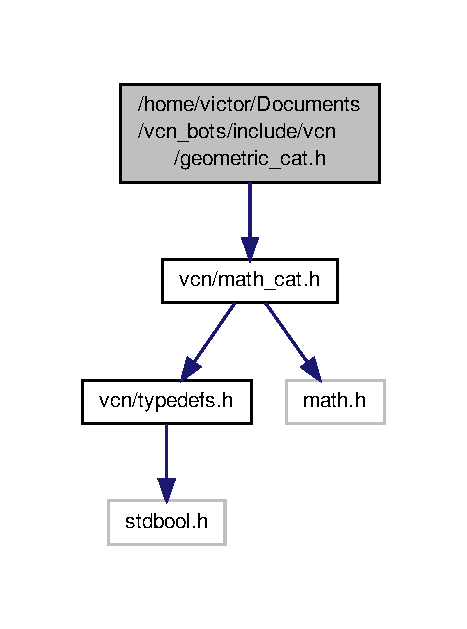
\includegraphics[width=224pt]{geometric__cat_8h__incl}
\end{center}
\end{figure}
\subsection*{Macros}
\begin{DoxyCompactItemize}
\item 
\hypertarget{geometric__cat_8h_ab20e95f5fb6286d6f41db6423cbdc26d}{\#define {\bfseries G\+E\+O\+M\+E\+T\+R\+I\+C\+\_\+\+T\+O\+L\+E\+R\+A\+N\+C\+E}~(1.\+5e-\/8)}\label{geometric__cat_8h_ab20e95f5fb6286d6f41db6423cbdc26d}

\item 
\hypertarget{geometric__cat_8h_a9461a1a37412f7c2382874c8b69a0c74}{\#define {\bfseries G\+E\+O\+M\+E\+T\+R\+I\+C\+\_\+\+T\+O\+L\+E\+R\+A\+N\+C\+E\+\_\+\+P\+O\+W2}~(2.\+25e-\/16)}\label{geometric__cat_8h_a9461a1a37412f7c2382874c8b69a0c74}

\end{DoxyCompactItemize}
\subsection*{Functions}
\begin{DoxyCompactItemize}
\item 
\hypertarget{geometric__cat_8h_ac91bf4d4c681d2b7c80e53a6cab32f35}{void {\bfseries get\+\_\+normal\+\_\+2\+D} (const double $\ast$const x1, const double $\ast$const x2, double $\ast$normal)}\label{geometric__cat_8h_ac91bf4d4c681d2b7c80e53a6cab32f35}

\item 
\hypertarget{geometric__cat_8h_a4ffbd20d7f8033791d19d3904bc3af2d}{double {\bfseries get\+\_\+dist\+Pow2} (const double $\ast$const \+\_\+\+\_\+restrict p1, const double $\ast$const \+\_\+\+\_\+restrict p2)}\label{geometric__cat_8h_a4ffbd20d7f8033791d19d3904bc3af2d}

\item 
\hypertarget{geometric__cat_8h_a4abc307fd8f09b27b7cfbfa5feec4841}{double {\bfseries get\+\_\+dist} (const double $\ast$const \+\_\+\+\_\+restrict p1, const double $\ast$const \+\_\+\+\_\+restrict p2)}\label{geometric__cat_8h_a4abc307fd8f09b27b7cfbfa5feec4841}

\item 
\hypertarget{geometric__cat_8h_a918b11d4fa32fb1d803f618821f71624}{void \hyperlink{geometric__cat_8h_a918b11d4fa32fb1d803f618821f71624}{vcn\+\_\+get\+\_\+enveloping\+\_\+box} (uint N\+\_\+vertices, const double $\ast$const vertices, double box\mbox{[}4\mbox{]})}\label{geometric__cat_8h_a918b11d4fa32fb1d803f618821f71624}

\begin{DoxyCompactList}\small\item\em Get enveloping box. \end{DoxyCompactList}\item 
\hypertarget{geometric__cat_8h_a3718606bed9ed1a5382a978d288fe455}{double {\bfseries get\+\_\+2triangle\+\_\+area} (const double $\ast$const \+\_\+\+\_\+restrict t1, const double $\ast$const \+\_\+\+\_\+restrict t2, const double $\ast$const \+\_\+\+\_\+restrict t3)}\label{geometric__cat_8h_a3718606bed9ed1a5382a978d288fe455}

\item 
\hypertarget{geometric__cat_8h_ac459c28100664311823ff0a5195e58c4}{void {\bfseries get\+\_\+triangle\+\_\+centroid} (const double $\ast$const \+\_\+\+\_\+restrict t1, const double $\ast$const \+\_\+\+\_\+restrict t2, const double $\ast$const \+\_\+\+\_\+restrict t3, double $\ast$const \+\_\+\+\_\+restrict centroid)}\label{geometric__cat_8h_ac459c28100664311823ff0a5195e58c4}

\item 
\hypertarget{geometric__cat_8h_a810401891169dbce4fb713bb05230cd0}{double {\bfseries get\+\_\+triangle\+\_\+min\+\_\+angle} (const double $\ast$const t1, const double $\ast$const t2, const double $\ast$const t3)}\label{geometric__cat_8h_a810401891169dbce4fb713bb05230cd0}

\item 
\hypertarget{geometric__cat_8h_a13b7cbc199dbc847fe2beefca9ad0d84}{double {\bfseries get\+\_\+triangle\+\_\+cr2se\+\_\+ratio} (const double $\ast$const t1, const double $\ast$const t2, const double $\ast$const t3)}\label{geometric__cat_8h_a13b7cbc199dbc847fe2beefca9ad0d84}

\item 
\hypertarget{geometric__cat_8h_a07ee069fe0a7966c9797da5335af36d2}{double {\bfseries get\+\_\+circumradius} (const double $\ast$const t1, const double $\ast$const t2, const double $\ast$const t3)}\label{geometric__cat_8h_a07ee069fe0a7966c9797da5335af36d2}

\item 
\hypertarget{geometric__cat_8h_a44fbea8fdc8a780028e5135f2e95386a}{void {\bfseries get\+\_\+circumcenter} (const double $\ast$const t1, const double $\ast$const t2, const double $\ast$const t3, double $\ast$const xc)}\label{geometric__cat_8h_a44fbea8fdc8a780028e5135f2e95386a}

\item 
\hypertarget{geometric__cat_8h_a588096a1a28b33a3eb64fab3e2d4bf3c}{void {\bfseries get\+\_\+circumcenter\+\_\+from\+\_\+segment} (const double $\ast$const s1, const double $\ast$const s2, double radii, double $\ast$const xc)}\label{geometric__cat_8h_a588096a1a28b33a3eb64fab3e2d4bf3c}

\item 
\hypertarget{geometric__cat_8h_a3e1f8601c1a6ee014e6675bc6d465801}{double {\bfseries get\+\_\+triangle\+\_\+quality} (const double $\ast$const t1, const double $\ast$const t2, const double $\ast$const t3)}\label{geometric__cat_8h_a3e1f8601c1a6ee014e6675bc6d465801}

\item 
\hypertarget{geometric__cat_8h_ac0fe1b1ffd9f898f38d06cf064f0b90a}{void {\bfseries get\+\_\+min\+\_\+and\+\_\+max\+\_\+lengths\+\_\+of\+\_\+the\+\_\+triangle\+\_\+sides} (const double $\ast$const t1, const double $\ast$const t2, const double $\ast$const t3, double $\ast$min, double $\ast$max)}\label{geometric__cat_8h_ac0fe1b1ffd9f898f38d06cf064f0b90a}

\item 
\hypertarget{geometric__cat_8h_a62f0c2256493246ffe77db126dd1a975}{uint {\bfseries get\+\_\+closest\+\_\+vertex} (const double $\ast$const vertices, uint N, double x, double y, uint N\+\_\+index\+\_\+to\+\_\+ignore, uint $\ast$index\+\_\+to\+\_\+ignore, double $\ast$distance)}\label{geometric__cat_8h_a62f0c2256493246ffe77db126dd1a975}

\item 
\hypertarget{geometric__cat_8h_a94017850cab80e982ac68bb723bbb143}{int {\bfseries get\+\_\+closest\+\_\+point\+\_\+to\+\_\+the\+\_\+segment} (const double $\ast$const s1, const double $\ast$const s2, const double $\ast$const p, double $\ast$const p\+\_\+closest)}\label{geometric__cat_8h_a94017850cab80e982ac68bb723bbb143}

\item 
\hypertarget{geometric__cat_8h_a1ec241bc3cd504c07e68af8441feb69a}{int {\bfseries get\+\_\+closest\+\_\+dist\+\_\+to\+\_\+the\+\_\+segment} (const double $\ast$const \+\_\+\+\_\+restrict s1, const double $\ast$const \+\_\+\+\_\+restrict s2, const double $\ast$const \+\_\+\+\_\+restrict p)}\label{geometric__cat_8h_a1ec241bc3cd504c07e68af8441feb69a}

\item 
\hypertarget{geometric__cat_8h_a9372990fef3bb31ec27ef8ac6eec4757}{bool {\bfseries does\+\_\+the\+\_\+segments\+\_\+are\+\_\+intersected} (const double $\ast$const sa1, const double $\ast$const sa2, const double $\ast$const sb1, const double $\ast$const sb2, double $\ast$const p\+\_\+out, int $\ast$const status)}\label{geometric__cat_8h_a9372990fef3bb31ec27ef8ac6eec4757}

\item 
\hypertarget{geometric__cat_8h_a608257fdea39ad026c2f48715d82dcac}{bool {\bfseries does\+\_\+the\+\_\+point\+\_\+lies\+\_\+upon\+\_\+the\+\_\+segment} (const double $\ast$const s1, const double $\ast$const s2, const double $\ast$const p)}\label{geometric__cat_8h_a608257fdea39ad026c2f48715d82dcac}

\item 
\hypertarget{geometric__cat_8h_a72d10fd1b88df41233868e80aeef4b42}{bool {\bfseries does\+\_\+the\+\_\+point\+\_\+lies\+\_\+in\+\_\+the\+\_\+triangle} (const double $\ast$const t1, const double $\ast$const t2, const double $\ast$const t3, const double $\ast$const p)}\label{geometric__cat_8h_a72d10fd1b88df41233868e80aeef4b42}

\item 
\hypertarget{geometric__cat_8h_a0f30ff9a832373ca89126946680d3035}{bool {\bfseries does\+\_\+the\+\_\+point\+\_\+lies\+\_\+inside\+\_\+the\+\_\+triangle} (const double $\ast$const t1, const double $\ast$const t2, const double $\ast$const t3, const double $\ast$const p)}\label{geometric__cat_8h_a0f30ff9a832373ca89126946680d3035}

\item 
\hypertarget{geometric__cat_8h_ad151ae4f746c1482b763410c7fc9793d}{bool {\bfseries does\+\_\+the\+\_\+point\+\_\+lies\+\_\+inside\+\_\+the\+\_\+diametral\+\_\+circle} (const double $\ast$const s1, const double $\ast$const s2, const double $\ast$const p)}\label{geometric__cat_8h_ad151ae4f746c1482b763410c7fc9793d}

\item 
\hypertarget{geometric__cat_8h_a5d127a40ebaa0fb797da0d91e2f1fc4d}{bool {\bfseries does\+\_\+the\+\_\+point\+\_\+lies\+\_\+inside\+\_\+the\+\_\+circumcircle} (const double $\ast$const t1, const double $\ast$const t2, const double $\ast$const t3, const double $\ast$const p)}\label{geometric__cat_8h_a5d127a40ebaa0fb797da0d91e2f1fc4d}

\item 
\hypertarget{geometric__cat_8h_ab285539a68aa429c85ff3cb08cc4ba37}{bool {\bfseries does\+\_\+the\+\_\+segment\+\_\+intersects\+\_\+the\+\_\+triangle} (const double $\ast$const t1, const double $\ast$const t2, const double $\ast$const t3, const double $\ast$const s1, const double $\ast$const s2)}\label{geometric__cat_8h_ab285539a68aa429c85ff3cb08cc4ba37}

\item 
\hypertarget{geometric__cat_8h_a9aa16a689c91727c230c0bb56aa5e168}{bool {\bfseries does\+\_\+the\+\_\+segment\+\_\+intersects\+\_\+the\+\_\+circle} (double $\ast$circumcenter, double radius, double $\ast$s1, double $\ast$s2)}\label{geometric__cat_8h_a9aa16a689c91727c230c0bb56aa5e168}

\item 
\hypertarget{geometric__cat_8h_ad6e2db07658d060936c732bb93611a58}{bool {\bfseries does\+\_\+the\+\_\+point\+\_\+lies\+\_\+inside\+\_\+the\+\_\+box} (const double $\ast$const bmin, const double $\ast$const bmax, const double $\ast$const p)}\label{geometric__cat_8h_ad6e2db07658d060936c732bb93611a58}

\end{DoxyCompactItemize}


\subsection{Detailed Description}
Simple geometric routines. 

\begin{DoxyAuthor}{Author}
Victor Eduardo Cardoso Nungaray ~\newline
 victorc@cimat.\+mx ~\newline
 \href{https://twitter.com/victore_cardoso}{\tt @victore\+\_\+cardoso } 
\end{DoxyAuthor}
\begin{DoxyDate}{Date}
10 August 2015
\end{DoxyDate}
\begin{DoxyParagraph}{License\+:}
This piece of code is in the P\+U\+B\+L\+I\+C D\+O\+M\+A\+I\+N, if your government does not recognizes such a dedication, then you are granted a perpetual and irrevocable license to copy and modify this file however you want. This does not imply any warranty. ~\newline
 Attributions and feedback are always welcome. 
\end{DoxyParagraph}

\hypertarget{graph__bot-coming__soon_8h}{\section{/home/victor/\+Documents/vcn\+\_\+bots/include/vcn/graph\+\_\+bot-\/coming\+\_\+soon.h File Reference}
\label{graph__bot-coming__soon_8h}\index{/home/victor/\+Documents/vcn\+\_\+bots/include/vcn/graph\+\_\+bot-\/coming\+\_\+soon.\+h@{/home/victor/\+Documents/vcn\+\_\+bots/include/vcn/graph\+\_\+bot-\/coming\+\_\+soon.\+h}}
}


Next features to be added to the Graph's Bot.  


\subsection*{Functions}
\begin{DoxyCompactItemize}
\item 
\hypertarget{graph__bot-coming__soon_8h_ab3967ef385306a83c1f3747f0101ac4f}{void {\bfseries vcn\+\_\+label\+\_\+minimum\+\_\+bandwidth} (uint N\+\_\+nodes, const uint $\ast$const N\+\_\+connections, uint $\ast$$\ast$connectivity\+\_\+matrix, uint $\ast$perm, uint $\ast$iperm)}\label{graph__bot-coming__soon_8h_ab3967ef385306a83c1f3747f0101ac4f}

\item 
\hypertarget{graph__bot-coming__soon_8h_aeb31fbc5d2d4bd578133e1188f3ff3c4}{void {\bfseries vcn\+\_\+label\+\_\+spectral} (uint N\+\_\+nodes, const uint $\ast$const N\+\_\+connections, uint $\ast$$\ast$connectivity\+\_\+matrix, uint $\ast$perm, uint $\ast$iperm)}\label{graph__bot-coming__soon_8h_aeb31fbc5d2d4bd578133e1188f3ff3c4}

\item 
\hypertarget{graph__bot-coming__soon_8h_a5adde6d64f7a1a44b0c1d97574afc4c8}{void {\bfseries vcn\+\_\+nested\+\_\+dissection} (uint N\+\_\+nodes, uint $\ast$N\+\_\+connections, uint $\ast$$\ast$connectivity\+\_\+matrix, uint $\ast$perm, uint $\ast$iperm)}\label{graph__bot-coming__soon_8h_a5adde6d64f7a1a44b0c1d97574afc4c8}

\end{DoxyCompactItemize}


\subsection{Detailed Description}
Next features to be added to the Graph's Bot. 

\begin{DoxyAuthor}{Author}
Victor Eduardo Cardoso Nungaray ~\newline
 victorc@cimat.\+mx ~\newline
 \href{https://twitter.com/victore_cardoso}{\tt @victore\+\_\+cardoso } 
\end{DoxyAuthor}
\begin{DoxyDate}{Date}
10 August 2015
\end{DoxyDate}
\begin{DoxyParagraph}{License\+:}
This piece of code is in the P\+U\+B\+L\+I\+C D\+O\+M\+A\+I\+N, if your government does not recognizes such a dedication, then you are granted a perpetual and irrevocable license to copy and modify this file however you want. This does not imply any warranty. ~\newline
 Attributions and feedback are always welcome. 
\end{DoxyParagraph}

\hypertarget{graph__bot_8h}{\section{/home/victor/\+Documents/vcn\+\_\+bots/include/vcn/graph\+\_\+bot.h File Reference}
\label{graph__bot_8h}\index{/home/victor/\+Documents/vcn\+\_\+bots/include/vcn/graph\+\_\+bot.\+h@{/home/victor/\+Documents/vcn\+\_\+bots/include/vcn/graph\+\_\+bot.\+h}}
}


The graph bot is a set of numerical procedures to handle graphs, exahistively used in meshing procedures, parallel computations and machine learning techniques.  


{\ttfamily \#include \char`\"{}vcn/typedefs.\+h\char`\"{}}\\*
Include dependency graph for graph\+\_\+bot.\+h\+:
\nopagebreak
\begin{figure}[H]
\begin{center}
\leavevmode
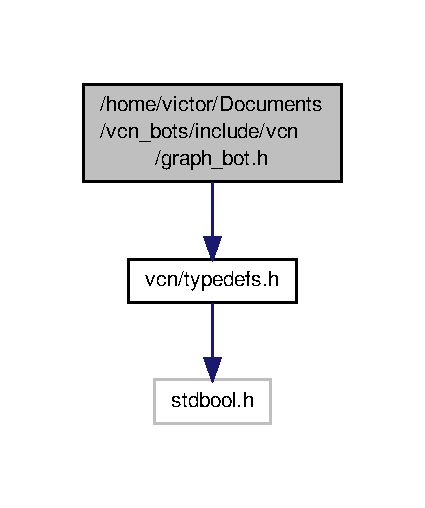
\includegraphics[width=204pt]{graph__bot_8h__incl}
\end{center}
\end{figure}
This graph shows which files directly or indirectly include this file\+:
\nopagebreak
\begin{figure}[H]
\begin{center}
\leavevmode
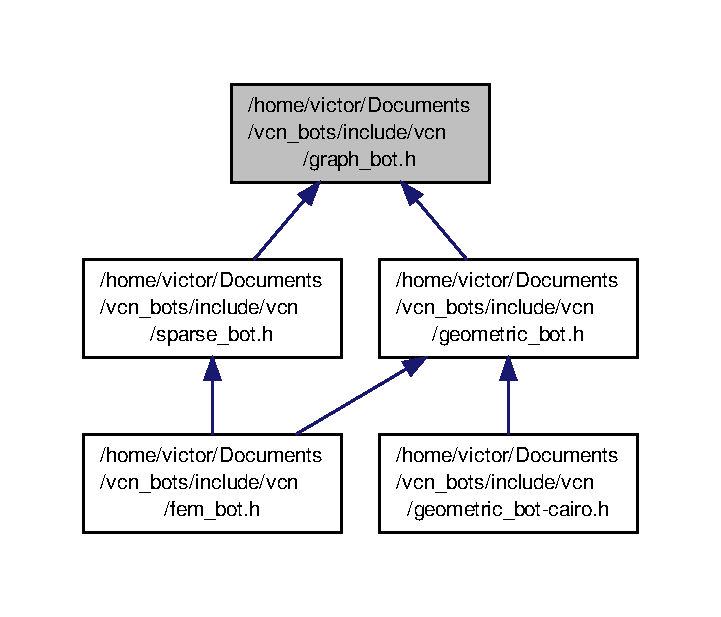
\includegraphics[width=346pt]{graph__bot_8h__dep__incl}
\end{center}
\end{figure}
\subsection*{Classes}
\begin{DoxyCompactItemize}
\item 
struct \hyperlink{structvcn__graph__s}{vcn\+\_\+graph\+\_\+s}
\begin{DoxyCompactList}\small\item\em Graph structure. \end{DoxyCompactList}\end{DoxyCompactItemize}
\subsection*{Typedefs}
\begin{DoxyCompactItemize}
\item 
\hypertarget{graph__bot_8h_a3a951da0c05a3e2ab67d73a94269fdab}{typedef struct \hyperlink{structvcn__graph__s}{vcn\+\_\+graph\+\_\+s} \hyperlink{graph__bot_8h_a3a951da0c05a3e2ab67d73a94269fdab}{vcn\+\_\+graph\+\_\+t}}\label{graph__bot_8h_a3a951da0c05a3e2ab67d73a94269fdab}

\begin{DoxyCompactList}\small\item\em Graph structure. \end{DoxyCompactList}\end{DoxyCompactItemize}
\subsection*{Functions}
\begin{DoxyCompactItemize}
\item 
void \hyperlink{graph__bot_8h_abc950f7fa0438a1ffcca287c553fe5ad}{vcn\+\_\+graph\+\_\+destroy} (\hyperlink{graph__bot_8h_a3a951da0c05a3e2ab67d73a94269fdab}{vcn\+\_\+graph\+\_\+t} $\ast$graph)
\begin{DoxyCompactList}\small\item\em Destroy graph. \end{DoxyCompactList}\item 
\hyperlink{graph__bot_8h_a3a951da0c05a3e2ab67d73a94269fdab}{vcn\+\_\+graph\+\_\+t} $\ast$ \hyperlink{graph__bot_8h_aed779f5201f689139f20428664dc3a2f}{vcn\+\_\+graph\+\_\+get\+\_\+subgraph} (const \hyperlink{graph__bot_8h_a3a951da0c05a3e2ab67d73a94269fdab}{vcn\+\_\+graph\+\_\+t} $\ast$const graph, uint N\+\_\+nodes, uint $\ast$nodes)
\begin{DoxyCompactList}\small\item\em Get a subgraph from the graph. \end{DoxyCompactList}\item 
uint $\ast$ \hyperlink{graph__bot_8h_a553a36280e5570478bb6db37903a1c03}{vcn\+\_\+graph\+\_\+labeling\+\_\+amd} (const \hyperlink{graph__bot_8h_a3a951da0c05a3e2ab67d73a94269fdab}{vcn\+\_\+graph\+\_\+t} $\ast$const graph, uint $\ast$iperm)
\begin{DoxyCompactList}\small\item\em Labeling used to minimize entries in L\+U decomposition based on the A\+M\+D algorithm. \end{DoxyCompactList}\item 
uint $\ast$ \hyperlink{graph__bot_8h_a22d4262265ef055e3fb4eed044540b6d}{vcn\+\_\+graph\+\_\+labeling\+\_\+mmd} (const \hyperlink{graph__bot_8h_a3a951da0c05a3e2ab67d73a94269fdab}{vcn\+\_\+graph\+\_\+t} $\ast$const graph, uint $\ast$iperm)
\begin{DoxyCompactList}\small\item\em Multiple Minimum Degree based on Quotient Graphs. The output labeling reduces the fill-\/in on L\+U decompositions. \end{DoxyCompactList}\item 
uint $\ast$ \hyperlink{graph__bot_8h_a3efa2fc387b77afe9debece16dd3a7aa}{vcn\+\_\+graph\+\_\+partition\+\_\+sb} (const \hyperlink{graph__bot_8h_a3a951da0c05a3e2ab67d73a94269fdab}{vcn\+\_\+graph\+\_\+t} $\ast$const graph, uint k)
\begin{DoxyCompactList}\small\item\em Graph partition using Spectral bisection. \end{DoxyCompactList}\end{DoxyCompactItemize}


\subsection{Detailed Description}
The graph bot is a set of numerical procedures to handle graphs, exahistively used in meshing procedures, parallel computations and machine learning techniques. 

\begin{DoxyAuthor}{Author}
Victor Eduardo Cardoso Nungaray ~\newline
 victorc@cimat.\+mx ~\newline
 \href{https://twitter.com/victore_cardoso}{\tt @victore\+\_\+cardoso } 
\end{DoxyAuthor}
\begin{DoxyDate}{Date}
10 August 2015
\end{DoxyDate}
\begin{DoxyParagraph}{License\+:}
This piece of code is in the P\+U\+B\+L\+I\+C D\+O\+M\+A\+I\+N, if your government does not recognizes such a dedication, then you are granted a perpetual and irrevocable license to copy and modify this file however you want. This does not imply any warranty. ~\newline
 Attributions and feedback are always welcome. 
\end{DoxyParagraph}


\subsection{Function Documentation}
\hypertarget{graph__bot_8h_abc950f7fa0438a1ffcca287c553fe5ad}{\index{graph\+\_\+bot.\+h@{graph\+\_\+bot.\+h}!vcn\+\_\+graph\+\_\+destroy@{vcn\+\_\+graph\+\_\+destroy}}
\index{vcn\+\_\+graph\+\_\+destroy@{vcn\+\_\+graph\+\_\+destroy}!graph\+\_\+bot.\+h@{graph\+\_\+bot.\+h}}
\subsubsection[{vcn\+\_\+graph\+\_\+destroy}]{\setlength{\rightskip}{0pt plus 5cm}void vcn\+\_\+graph\+\_\+destroy (
\begin{DoxyParamCaption}
\item[{{\bf vcn\+\_\+graph\+\_\+t} $\ast$}]{graph}
\end{DoxyParamCaption}
)}}\label{graph__bot_8h_abc950f7fa0438a1ffcca287c553fe5ad}


Destroy graph. 


\begin{DoxyParams}[1]{Parameters}
\mbox{\tt in}  & {\em graph} & Graph to be destroyed. \\
\hline
\end{DoxyParams}
\hypertarget{graph__bot_8h_aed779f5201f689139f20428664dc3a2f}{\index{graph\+\_\+bot.\+h@{graph\+\_\+bot.\+h}!vcn\+\_\+graph\+\_\+get\+\_\+subgraph@{vcn\+\_\+graph\+\_\+get\+\_\+subgraph}}
\index{vcn\+\_\+graph\+\_\+get\+\_\+subgraph@{vcn\+\_\+graph\+\_\+get\+\_\+subgraph}!graph\+\_\+bot.\+h@{graph\+\_\+bot.\+h}}
\subsubsection[{vcn\+\_\+graph\+\_\+get\+\_\+subgraph}]{\setlength{\rightskip}{0pt plus 5cm}{\bf vcn\+\_\+graph\+\_\+t}$\ast$ vcn\+\_\+graph\+\_\+get\+\_\+subgraph (
\begin{DoxyParamCaption}
\item[{const {\bf vcn\+\_\+graph\+\_\+t} $\ast$const}]{graph, }
\item[{uint}]{N\+\_\+nodes, }
\item[{uint $\ast$}]{nodes}
\end{DoxyParamCaption}
)}}\label{graph__bot_8h_aed779f5201f689139f20428664dc3a2f}


Get a subgraph from the graph. 


\begin{DoxyParams}[1]{Parameters}
\mbox{\tt in}  & {\em graph} & Super graph containing the output subgraph. \\
\hline
\mbox{\tt in}  & {\em N\+\_\+nodes} & Number of nodes in the subgraph. \\
\hline
\mbox{\tt in}  & {\em nodes} & I\+D of nodes of the subgraph. \\
\hline
\end{DoxyParams}
\begin{DoxyReturn}{Returns}
Subgraph. 
\end{DoxyReturn}
\hypertarget{graph__bot_8h_a553a36280e5570478bb6db37903a1c03}{\index{graph\+\_\+bot.\+h@{graph\+\_\+bot.\+h}!vcn\+\_\+graph\+\_\+labeling\+\_\+amd@{vcn\+\_\+graph\+\_\+labeling\+\_\+amd}}
\index{vcn\+\_\+graph\+\_\+labeling\+\_\+amd@{vcn\+\_\+graph\+\_\+labeling\+\_\+amd}!graph\+\_\+bot.\+h@{graph\+\_\+bot.\+h}}
\subsubsection[{vcn\+\_\+graph\+\_\+labeling\+\_\+amd}]{\setlength{\rightskip}{0pt plus 5cm}uint$\ast$ vcn\+\_\+graph\+\_\+labeling\+\_\+amd (
\begin{DoxyParamCaption}
\item[{const {\bf vcn\+\_\+graph\+\_\+t} $\ast$const}]{graph, }
\item[{uint $\ast$}]{iperm}
\end{DoxyParamCaption}
)}}\label{graph__bot_8h_a553a36280e5570478bb6db37903a1c03}


Labeling used to minimize entries in L\+U decomposition based on the A\+M\+D algorithm. 


\begin{DoxyParams}[1]{Parameters}
\mbox{\tt in}  & {\em graph} & Input graph to be labeled. \\
\hline
\mbox{\tt out}  & {\em iperm} & Inverse permutation, array mapping output I\+Ds with input I\+Ds. N\+U\+L\+L if not required. \\
\hline
\end{DoxyParams}
\begin{DoxyReturn}{Returns}
The permutation, an array mapping input I\+Ds with output I\+Ds.
\end{DoxyReturn}
\begin{DoxySeeAlso}{See also}
P. R. Amestoy, T. A. Davis and I. S. Duff. {\bfseries An Approximate Minimum Degree Ordering Algorithm.} Journal of Matrix Analysis and Applications (Vol. 17 1996), S\+I\+A\+M, pages 886-\/905. 
\end{DoxySeeAlso}
\hypertarget{graph__bot_8h_a22d4262265ef055e3fb4eed044540b6d}{\index{graph\+\_\+bot.\+h@{graph\+\_\+bot.\+h}!vcn\+\_\+graph\+\_\+labeling\+\_\+mmd@{vcn\+\_\+graph\+\_\+labeling\+\_\+mmd}}
\index{vcn\+\_\+graph\+\_\+labeling\+\_\+mmd@{vcn\+\_\+graph\+\_\+labeling\+\_\+mmd}!graph\+\_\+bot.\+h@{graph\+\_\+bot.\+h}}
\subsubsection[{vcn\+\_\+graph\+\_\+labeling\+\_\+mmd}]{\setlength{\rightskip}{0pt plus 5cm}uint$\ast$ vcn\+\_\+graph\+\_\+labeling\+\_\+mmd (
\begin{DoxyParamCaption}
\item[{const {\bf vcn\+\_\+graph\+\_\+t} $\ast$const}]{graph, }
\item[{uint $\ast$}]{iperm}
\end{DoxyParamCaption}
)}}\label{graph__bot_8h_a22d4262265ef055e3fb4eed044540b6d}


Multiple Minimum Degree based on Quotient Graphs. The output labeling reduces the fill-\/in on L\+U decompositions. 


\begin{DoxyParams}[1]{Parameters}
\mbox{\tt in}  & {\em graph} & Input graph to be labeled. \\
\hline
\mbox{\tt out}  & {\em iperm} & Inverse permutation, array mapping output I\+Ds with input I\+Ds. N\+U\+L\+L if not required. \\
\hline
\end{DoxyParams}
\begin{DoxyReturn}{Returns}
The permutation, an array mapping input I\+Ds with output I\+Ds.
\end{DoxyReturn}
\begin{DoxySeeAlso}{See also}
A. George and J. W.\+H. Liu. {\bfseries The evolution of the minimum degree ordering algorithm.} S\+I\+A\+M Review (Vol. 31 1989), pages 1-\/19. 
\end{DoxySeeAlso}
\hypertarget{graph__bot_8h_a3efa2fc387b77afe9debece16dd3a7aa}{\index{graph\+\_\+bot.\+h@{graph\+\_\+bot.\+h}!vcn\+\_\+graph\+\_\+partition\+\_\+sb@{vcn\+\_\+graph\+\_\+partition\+\_\+sb}}
\index{vcn\+\_\+graph\+\_\+partition\+\_\+sb@{vcn\+\_\+graph\+\_\+partition\+\_\+sb}!graph\+\_\+bot.\+h@{graph\+\_\+bot.\+h}}
\subsubsection[{vcn\+\_\+graph\+\_\+partition\+\_\+sb}]{\setlength{\rightskip}{0pt plus 5cm}uint$\ast$ vcn\+\_\+graph\+\_\+partition\+\_\+sb (
\begin{DoxyParamCaption}
\item[{const {\bf vcn\+\_\+graph\+\_\+t} $\ast$const}]{graph, }
\item[{uint}]{k}
\end{DoxyParamCaption}
)}}\label{graph__bot_8h_a3efa2fc387b77afe9debece16dd3a7aa}


Graph partition using Spectral bisection. 


\begin{DoxyParams}[1]{Parameters}
\mbox{\tt in}  & {\em graph} & Graph to be partitioned. \\
\hline
\end{DoxyParams}
\begin{DoxyReturn}{Returns}
Arrays of I\+Ds corresponding to the partition of each node, starting from zero.
\end{DoxyReturn}
\begin{DoxySeeAlso}{See also}
B. Hendrickson and R. Leland. {\bfseries An improved spectral graph partitioning algorithm for mapping parallel computations.} S\+I\+A\+M J. Sci. Comput. (Vol 16 1995), pages 452-\/469. 
\end{DoxySeeAlso}

\hypertarget{math__cat_8h}{\section{/home/victor/\+Documents/vcn\+\_\+bots/include/vcn/math\+\_\+cat.h File Reference}
\label{math__cat_8h}\index{/home/victor/\+Documents/vcn\+\_\+bots/include/vcn/math\+\_\+cat.\+h@{/home/victor/\+Documents/vcn\+\_\+bots/include/vcn/math\+\_\+cat.\+h}}
}


Simple math routines.  


{\ttfamily \#include \char`\"{}vcn/typedefs.\+h\char`\"{}}\\*
{\ttfamily \#include $<$math.\+h$>$}\\*
Include dependency graph for math\+\_\+cat.\+h\+:
\nopagebreak
\begin{figure}[H]
\begin{center}
\leavevmode
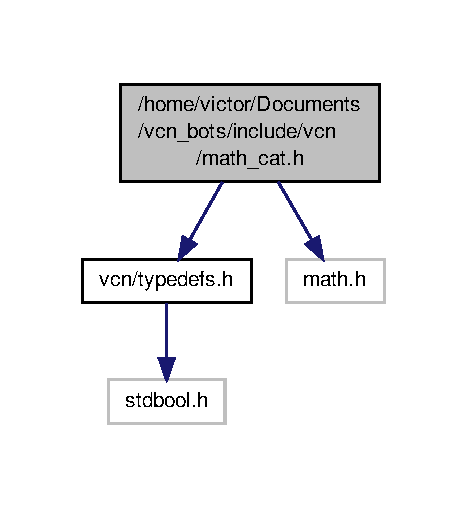
\includegraphics[width=224pt]{math__cat_8h__incl}
\end{center}
\end{figure}
This graph shows which files directly or indirectly include this file\+:
\nopagebreak
\begin{figure}[H]
\begin{center}
\leavevmode
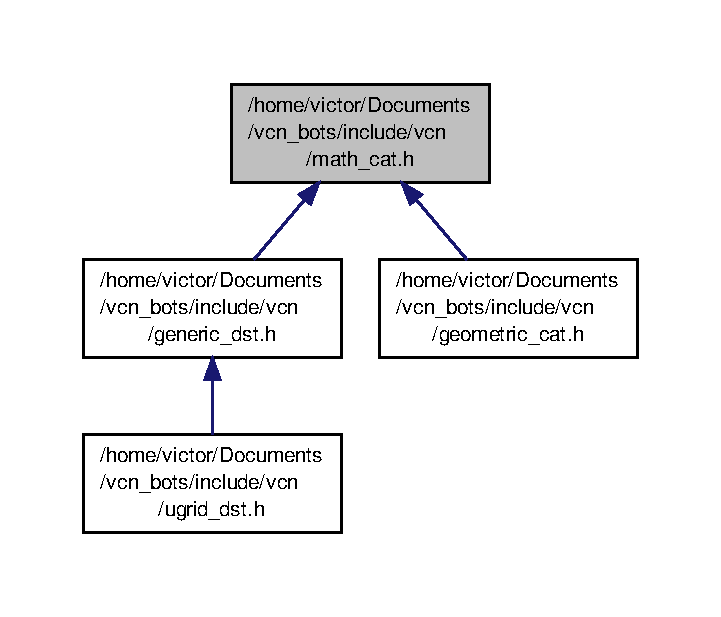
\includegraphics[width=346pt]{math__cat_8h__dep__incl}
\end{center}
\end{figure}
\subsection*{Classes}
\begin{DoxyCompactItemize}
\item 
struct \hyperlink{structGauss__Legendre__table__t}{Gauss\+\_\+\+Legendre\+\_\+table\+\_\+t}
\end{DoxyCompactItemize}
\subsection*{Macros}
\begin{DoxyCompactItemize}
\item 
\hypertarget{math__cat_8h_ae71449b1cc6e6250b91f539153a7a0d3}{\#define {\bfseries M\+\_\+\+P\+I}~(3.\+14159265358979323846264338327)}\label{math__cat_8h_ae71449b1cc6e6250b91f539153a7a0d3}

\item 
\hypertarget{math__cat_8h_ab1fb5556708bdfa9e495e77c26b83b49}{\#define {\bfseries M\+A\+X\+\_\+\+U\+I\+N\+T}~((unsigned int)(-\/1))}\label{math__cat_8h_ab1fb5556708bdfa9e495e77c26b83b49}

\item 
\hypertarget{math__cat_8h_a514396dd60fa0621c83072091fb2a0cd}{\#define {\bfseries S\+Q\+R\+T2}~(1.\+41421356237309504880)}\label{math__cat_8h_a514396dd60fa0621c83072091fb2a0cd}

\item 
\hypertarget{math__cat_8h_ae42978afd835c3a1f70d409a1b5f5a39}{\#define {\bfseries S\+Q\+R\+T3}~(1.\+73205080756887729352)}\label{math__cat_8h_ae42978afd835c3a1f70d409a1b5f5a39}

\item 
\hypertarget{math__cat_8h_a5c61eeb300e28e2d68938ed36640177a}{\#define {\bfseries I\+N\+V\+\_\+\+S\+Q\+R\+T3}~(0.\+57735026919)  /$\ast$ 1/sqrt(3) $\ast$/}\label{math__cat_8h_a5c61eeb300e28e2d68938ed36640177a}

\item 
\hypertarget{math__cat_8h_ae869c70a21a4f1b096c1d0ef699d3c30}{\#define {\bfseries I\+N\+V\+\_\+\+S\+Q\+R\+T6}~(0.\+40824829046)  /$\ast$ 1/sqrt(6) $\ast$/}\label{math__cat_8h_ae869c70a21a4f1b096c1d0ef699d3c30}

\end{DoxyCompactItemize}
\subsection*{Functions}
\begin{DoxyCompactItemize}
\item 
\hypertarget{math__cat_8h_aeaccc39baa3a109dc36ab7939c110c60}{int {\bfseries pow2i} (int a)}\label{math__cat_8h_aeaccc39baa3a109dc36ab7939c110c60}

\item 
\hypertarget{math__cat_8h_a2cd7f59510dbcdad5f6526fc7ef08853}{int {\bfseries powk} (int a, uint k)}\label{math__cat_8h_a2cd7f59510dbcdad5f6526fc7ef08853}

\item 
\hypertarget{math__cat_8h_a4136222d97588360c5b5ed9735e0b670}{uint {\bfseries pow2u} (uint a)}\label{math__cat_8h_a4136222d97588360c5b5ed9735e0b670}

\item 
\hypertarget{math__cat_8h_a87f1b0ee3570dee48d6bb9739e8b75df}{double {\bfseries pow2} (double a)}\label{math__cat_8h_a87f1b0ee3570dee48d6bb9739e8b75df}

\item 
\hypertarget{math__cat_8h_a5f945dd59574be1d9270a9bf1be8bb2a}{double {\bfseries pow3} (double a)}\label{math__cat_8h_a5f945dd59574be1d9270a9bf1be8bb2a}

\item 
\hypertarget{math__cat_8h_a95e2963ee3caed51c04dd8c6129b062a}{double {\bfseries pow4} (double a)}\label{math__cat_8h_a95e2963ee3caed51c04dd8c6129b062a}

\item 
\hypertarget{math__cat_8h_ae4432a69291e3f77a2f580b9ae18106a}{double {\bfseries pow5} (double a)}\label{math__cat_8h_ae4432a69291e3f77a2f580b9ae18106a}

\item 
\hypertarget{math__cat_8h_a73bfd0b195aa24e88a64710065b5f13a}{double {\bfseries pow6} (double a)}\label{math__cat_8h_a73bfd0b195aa24e88a64710065b5f13a}

\item 
\hypertarget{math__cat_8h_a43d02bb809bacde5e093c7310587c56c}{double {\bfseries pow7} (double a)}\label{math__cat_8h_a43d02bb809bacde5e093c7310587c56c}

\item 
\hypertarget{math__cat_8h_a0ff8a661089e66ad9b4f02d7ba118dee}{double {\bfseries pow8} (double a)}\label{math__cat_8h_a0ff8a661089e66ad9b4f02d7ba118dee}

\item 
\hypertarget{math__cat_8h_a94bd2fb872789d150df4e533bbcaebc9}{double {\bfseries pow9} (double a)}\label{math__cat_8h_a94bd2fb872789d150df4e533bbcaebc9}

\item 
\hypertarget{math__cat_8h_abd8bbcfabb3ddef2ccaafb9928a37b95}{int {\bfseries min} (int a, int b)}\label{math__cat_8h_abd8bbcfabb3ddef2ccaafb9928a37b95}

\item 
\hypertarget{math__cat_8h_af082905f7eac6d03e92015146bbc1925}{int {\bfseries max} (int a, int b)}\label{math__cat_8h_af082905f7eac6d03e92015146bbc1925}

\item 
\hypertarget{math__cat_8h_acaa6dc0b0c9d374a9169eddc348cfd80}{uint {\bfseries minu} (uint a, uint b)}\label{math__cat_8h_acaa6dc0b0c9d374a9169eddc348cfd80}

\item 
\hypertarget{math__cat_8h_a48d788e32c73734b54387c036d38180a}{uint {\bfseries maxu} (uint a, uint b)}\label{math__cat_8h_a48d788e32c73734b54387c036d38180a}

\item 
\hypertarget{math__cat_8h_aca86432a644e6fe95e8e800646056522}{double {\bfseries mind} (double a, double b)}\label{math__cat_8h_aca86432a644e6fe95e8e800646056522}

\item 
\hypertarget{math__cat_8h_a44382b42eb4cbc06b090262941f6b52e}{double {\bfseries maxd} (double a, double b)}\label{math__cat_8h_a44382b42eb4cbc06b090262941f6b52e}

\item 
\hypertarget{math__cat_8h_aa1440c5d16aa5fa9549eff1af2f36783}{double {\bfseries hypotenuse} (double a, double b)}\label{math__cat_8h_aa1440c5d16aa5fa9549eff1af2f36783}

\item 
\hypertarget{math__cat_8h_aed4fee868c9f7050b48fe50339a08ed0}{double {\bfseries get\+\_\+harmonic\+\_\+average} (double a, double b)}\label{math__cat_8h_aed4fee868c9f7050b48fe50339a08ed0}

\item 
\hypertarget{math__cat_8h_ad6b278c9c8d3326a9f649671cd826e28}{\hyperlink{structGauss__Legendre__table__t}{Gauss\+\_\+\+Legendre\+\_\+table\+\_\+t} $\ast$ {\bfseries G\+Ltable\+\_\+create} (uint N\+\_\+points)}\label{math__cat_8h_ad6b278c9c8d3326a9f649671cd826e28}

\item 
\hypertarget{math__cat_8h_accaadaedc40a0acab6de2f611770e1bf}{void {\bfseries G\+Ltable\+\_\+destroy} (\hyperlink{structGauss__Legendre__table__t}{Gauss\+\_\+\+Legendre\+\_\+table\+\_\+t} $\ast$G\+Ltable)}\label{math__cat_8h_accaadaedc40a0acab6de2f611770e1bf}

\end{DoxyCompactItemize}


\subsection{Detailed Description}
Simple math routines. 

\begin{DoxyAuthor}{Author}
Victor Eduardo Cardoso Nungaray ~\newline
 victorc@cimat.\+mx ~\newline
 \href{https://twitter.com/victore_cardoso}{\tt @victore\+\_\+cardoso } 
\end{DoxyAuthor}
\begin{DoxyDate}{Date}
10 August 2015
\end{DoxyDate}
\begin{DoxyParagraph}{License\+:}
This piece of code is in the P\+U\+B\+L\+I\+C D\+O\+M\+A\+I\+N, if your government does not recognizes such a dedication, then you are granted a perpetual and irrevocable license to copy and modify this file however you want. This does not imply any warranty. ~\newline
 Attributions and feedback are always welcome. 
\end{DoxyParagraph}

\hypertarget{sparse__bot_8h}{\section{/home/victor/\+Documents/vcn\+\_\+bots/include/vcn/sparse\+\_\+bot.h File Reference}
\label{sparse__bot_8h}\index{/home/victor/\+Documents/vcn\+\_\+bots/include/vcn/sparse\+\_\+bot.\+h@{/home/victor/\+Documents/vcn\+\_\+bots/include/vcn/sparse\+\_\+bot.\+h}}
}


The sparse bot is a set of solvers for symmetric and sparse matrices. There are fast matrix computations.  


{\ttfamily \#include \char`\"{}vcn/typedefs.\+h\char`\"{}}\\*
{\ttfamily \#include \char`\"{}vcn/graph\+\_\+bot.\+h\char`\"{}}\\*
Include dependency graph for sparse\+\_\+bot.\+h\+:
\nopagebreak
\begin{figure}[H]
\begin{center}
\leavevmode
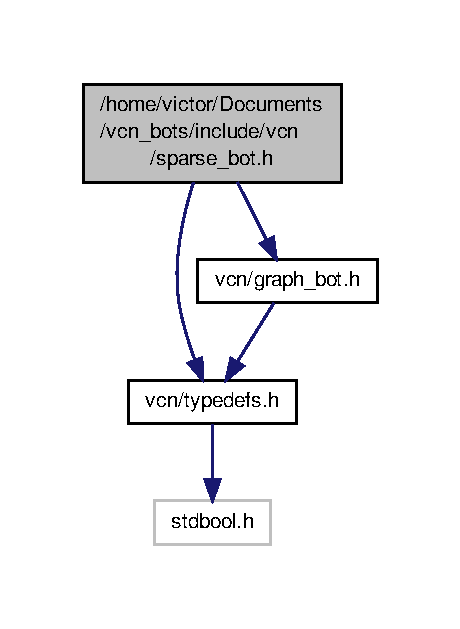
\includegraphics[width=221pt]{sparse__bot_8h__incl}
\end{center}
\end{figure}
This graph shows which files directly or indirectly include this file\+:
\nopagebreak
\begin{figure}[H]
\begin{center}
\leavevmode
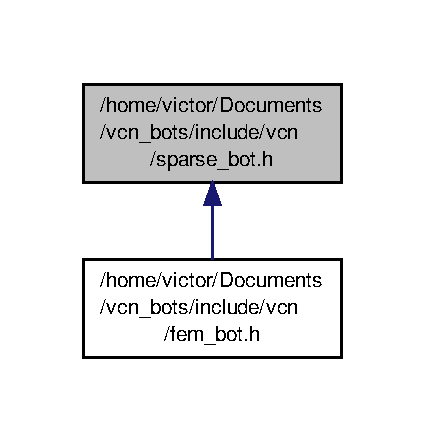
\includegraphics[width=204pt]{sparse__bot_8h__dep__incl}
\end{center}
\end{figure}
\subsection*{Macros}
\begin{DoxyCompactItemize}
\item 
\hypertarget{sparse__bot_8h_a5b6ff826c42f9186e4089e274087e3a2}{\#define \hyperlink{sparse__bot_8h_a5b6ff826c42f9186e4089e274087e3a2}{V\+C\+N\+\_\+\+S\+O\+L\+V\+E\+R\+\_\+\+L\+U\+D}~(1)}\label{sparse__bot_8h_a5b6ff826c42f9186e4089e274087e3a2}

\begin{DoxyCompactList}\small\item\em L\+U decomposition. \end{DoxyCompactList}\item 
\hypertarget{sparse__bot_8h_a943bf6aaf7a80125dd7ae5b366092547}{\#define \hyperlink{sparse__bot_8h_a943bf6aaf7a80125dd7ae5b366092547}{V\+C\+N\+\_\+\+S\+O\+L\+V\+E\+R\+\_\+\+C\+H\+K}~(2)}\label{sparse__bot_8h_a943bf6aaf7a80125dd7ae5b366092547}

\begin{DoxyCompactList}\small\item\em Cholesky decomposition. \end{DoxyCompactList}\item 
\hypertarget{sparse__bot_8h_ab6d21df2c8203b527cfa41e109aab996}{\#define \hyperlink{sparse__bot_8h_ab6d21df2c8203b527cfa41e109aab996}{V\+C\+N\+\_\+\+S\+O\+L\+V\+E\+R\+\_\+\+C\+G\+J}~(3)}\label{sparse__bot_8h_ab6d21df2c8203b527cfa41e109aab996}

\begin{DoxyCompactList}\small\item\em Conjugate Gradient preconditioned with Jacobi. \end{DoxyCompactList}\end{DoxyCompactItemize}
\subsection*{Typedefs}
\begin{DoxyCompactItemize}
\item 
\hypertarget{sparse__bot_8h_a7e7199ab50f88583be4e2c093ede990d}{typedef struct vcn\+\_\+sparse\+\_\+s \hyperlink{sparse__bot_8h_a7e7199ab50f88583be4e2c093ede990d}{vcn\+\_\+sparse\+\_\+t}}\label{sparse__bot_8h_a7e7199ab50f88583be4e2c093ede990d}

\begin{DoxyCompactList}\small\item\em Sparse matrix in \char`\"{}\+Compress Row Storage\char`\"{} format. \end{DoxyCompactList}\end{DoxyCompactItemize}
\subsection*{Functions}
\begin{DoxyCompactItemize}
\item 
\hyperlink{sparse__bot_8h_a7e7199ab50f88583be4e2c093ede990d}{vcn\+\_\+sparse\+\_\+t} $\ast$ \hyperlink{sparse__bot_8h_a27a8168cd7853bcb1b03ccc926aa436b}{vcn\+\_\+sparse\+\_\+create} (const \hyperlink{graph__bot_8h_a3a951da0c05a3e2ab67d73a94269fdab}{vcn\+\_\+graph\+\_\+t} $\ast$const graph, const uint $\ast$const perm, uint vars\+\_\+per\+\_\+node)
\begin{DoxyCompactList}\small\item\em Create a sparse matrix from a graph. \end{DoxyCompactList}\item 
\hypertarget{sparse__bot_8h_a46557bd0aa9e52335fb0fefd32fa637a}{\hyperlink{sparse__bot_8h_a7e7199ab50f88583be4e2c093ede990d}{vcn\+\_\+sparse\+\_\+t} $\ast$ {\bfseries vcn\+\_\+sparse\+\_\+clone} (\hyperlink{sparse__bot_8h_a7e7199ab50f88583be4e2c093ede990d}{vcn\+\_\+sparse\+\_\+t} $\ast$A)}\label{sparse__bot_8h_a46557bd0aa9e52335fb0fefd32fa637a}

\item 
\hypertarget{sparse__bot_8h_a5967196046f509a0099ed6c33e11a43f}{void {\bfseries vcn\+\_\+sparse\+\_\+save} (const \hyperlink{sparse__bot_8h_a7e7199ab50f88583be4e2c093ede990d}{vcn\+\_\+sparse\+\_\+t} $\ast$const A, const char $\ast$filename)}\label{sparse__bot_8h_a5967196046f509a0099ed6c33e11a43f}

\item 
\hypertarget{sparse__bot_8h_aa9517799b72d86621769d1bb2739eb3d}{void {\bfseries vcn\+\_\+sparse\+\_\+destroy} (\hyperlink{sparse__bot_8h_a7e7199ab50f88583be4e2c093ede990d}{vcn\+\_\+sparse\+\_\+t} $\ast$A)}\label{sparse__bot_8h_aa9517799b72d86621769d1bb2739eb3d}

\item 
\hypertarget{sparse__bot_8h_a79c7397201890dc77d10e5fda87f5267}{void {\bfseries vcn\+\_\+sparse\+\_\+reset} (\hyperlink{sparse__bot_8h_a7e7199ab50f88583be4e2c093ede990d}{vcn\+\_\+sparse\+\_\+t} $\ast$A)}\label{sparse__bot_8h_a79c7397201890dc77d10e5fda87f5267}

\item 
\hypertarget{sparse__bot_8h_af7423014075b89eeecddceed54d3744f}{void {\bfseries vcn\+\_\+sparse\+\_\+set} (\hyperlink{sparse__bot_8h_a7e7199ab50f88583be4e2c093ede990d}{vcn\+\_\+sparse\+\_\+t} $\ast$A, uint i, uint j, double value)}\label{sparse__bot_8h_af7423014075b89eeecddceed54d3744f}

\item 
\hypertarget{sparse__bot_8h_a445cc09b48e389ff78bf98a89e88d73a}{void {\bfseries vcn\+\_\+sparse\+\_\+set\+\_\+identity\+\_\+row} (\hyperlink{sparse__bot_8h_a7e7199ab50f88583be4e2c093ede990d}{vcn\+\_\+sparse\+\_\+t} $\ast$A, uint row)}\label{sparse__bot_8h_a445cc09b48e389ff78bf98a89e88d73a}

\item 
\hypertarget{sparse__bot_8h_afa5145286ea1e6550b07a7be48dbe573}{void {\bfseries vcn\+\_\+sparse\+\_\+make\+\_\+diagonal} (\hyperlink{sparse__bot_8h_a7e7199ab50f88583be4e2c093ede990d}{vcn\+\_\+sparse\+\_\+t} $\ast$A, double diag\+\_\+val)}\label{sparse__bot_8h_afa5145286ea1e6550b07a7be48dbe573}

\item 
\hypertarget{sparse__bot_8h_ac0b904ca7bbe2fbeb588ba4edabe5cd3}{double {\bfseries vcn\+\_\+sparse\+\_\+get} (const \hyperlink{sparse__bot_8h_a7e7199ab50f88583be4e2c093ede990d}{vcn\+\_\+sparse\+\_\+t} $\ast$const A, uint i, uint j)}\label{sparse__bot_8h_ac0b904ca7bbe2fbeb588ba4edabe5cd3}

\item 
\hypertarget{sparse__bot_8h_af705ac7b904a5a03a5991e92013583cf}{double {\bfseries vcn\+\_\+sparse\+\_\+get\+\_\+and\+\_\+set} (\hyperlink{sparse__bot_8h_a7e7199ab50f88583be4e2c093ede990d}{vcn\+\_\+sparse\+\_\+t} $\ast$A, uint i, uint j, double value)}\label{sparse__bot_8h_af705ac7b904a5a03a5991e92013583cf}

\item 
\hypertarget{sparse__bot_8h_ade162e8689a7f8b2cf2c0dc4a992b146}{bool {\bfseries vcn\+\_\+sparse\+\_\+is\+\_\+non\+\_\+zero} (const \hyperlink{sparse__bot_8h_a7e7199ab50f88583be4e2c093ede990d}{vcn\+\_\+sparse\+\_\+t} $\ast$const A, uint i, uint j)}\label{sparse__bot_8h_ade162e8689a7f8b2cf2c0dc4a992b146}

\item 
\hypertarget{sparse__bot_8h_af3bfab7303daa9f705a8f6bd89d273c2}{uint {\bfseries vcn\+\_\+sparse\+\_\+memory\+\_\+used} (const \hyperlink{sparse__bot_8h_a7e7199ab50f88583be4e2c093ede990d}{vcn\+\_\+sparse\+\_\+t} $\ast$const A)}\label{sparse__bot_8h_af3bfab7303daa9f705a8f6bd89d273c2}

\item 
\hypertarget{sparse__bot_8h_afc156c86d54abbc5d88e2229534081ee}{void {\bfseries vcn\+\_\+sparse\+\_\+add} (\hyperlink{sparse__bot_8h_a7e7199ab50f88583be4e2c093ede990d}{vcn\+\_\+sparse\+\_\+t} $\ast$A, uint i, uint j, double value)}\label{sparse__bot_8h_afc156c86d54abbc5d88e2229534081ee}

\item 
\hypertarget{sparse__bot_8h_aa5106d2051bec6738fadcfe69d2800f2}{void {\bfseries vcn\+\_\+sparse\+\_\+scale} (\hyperlink{sparse__bot_8h_a7e7199ab50f88583be4e2c093ede990d}{vcn\+\_\+sparse\+\_\+t} $\ast$A, double factor)}\label{sparse__bot_8h_aa5106d2051bec6738fadcfe69d2800f2}

\item 
\hypertarget{sparse__bot_8h_ac4f789b247182fd354d9c9579c2fbd28}{void {\bfseries vcn\+\_\+sparse\+\_\+transpose} (\hyperlink{sparse__bot_8h_a7e7199ab50f88583be4e2c093ede990d}{vcn\+\_\+sparse\+\_\+t} $\ast$A, \hyperlink{sparse__bot_8h_a7e7199ab50f88583be4e2c093ede990d}{vcn\+\_\+sparse\+\_\+t} $\ast$\+\_\+\+At)}\label{sparse__bot_8h_ac4f789b247182fd354d9c9579c2fbd28}

\item 
\hypertarget{sparse__bot_8h_a6c3998747413482413a108bb4103c5ab}{uint {\bfseries vcn\+\_\+sparse\+\_\+get\+\_\+size} (const \hyperlink{sparse__bot_8h_a7e7199ab50f88583be4e2c093ede990d}{vcn\+\_\+sparse\+\_\+t} $\ast$const A)}\label{sparse__bot_8h_a6c3998747413482413a108bb4103c5ab}

\item 
\hypertarget{sparse__bot_8h_adaeb0625a8d4cd1de4963ff36dd8824f}{uint {\bfseries vcn\+\_\+sparse\+\_\+get\+\_\+nnz} (const \hyperlink{sparse__bot_8h_a7e7199ab50f88583be4e2c093ede990d}{vcn\+\_\+sparse\+\_\+t} $\ast$const A)}\label{sparse__bot_8h_adaeb0625a8d4cd1de4963ff36dd8824f}

\item 
\hypertarget{sparse__bot_8h_a07c82209ccbffa4e2448364d4bbdd92c}{void {\bfseries vcn\+\_\+sparse\+\_\+multiply\+\_\+scalar} (\hyperlink{sparse__bot_8h_a7e7199ab50f88583be4e2c093ede990d}{vcn\+\_\+sparse\+\_\+t} $\ast$A, double scalar, uint omp\+\_\+parallel\+\_\+threads)}\label{sparse__bot_8h_a07c82209ccbffa4e2448364d4bbdd92c}

\item 
\hypertarget{sparse__bot_8h_aaf07cfd5b4442d9a1c6e1f50c653b52a}{void {\bfseries vcn\+\_\+sparse\+\_\+multiply\+\_\+vector} (\hyperlink{sparse__bot_8h_a7e7199ab50f88583be4e2c093ede990d}{vcn\+\_\+sparse\+\_\+t} $\ast$A, double $\ast$in, double $\ast$out, uint omp\+\_\+parallel\+\_\+threads)}\label{sparse__bot_8h_aaf07cfd5b4442d9a1c6e1f50c653b52a}

\item 
\hypertarget{sparse__bot_8h_a7f6c99882fdb87089267ee8a7c052fd5}{void {\bfseries vcn\+\_\+sparse\+\_\+set\+\_\+\+Dirichlet\+\_\+condition} (\hyperlink{sparse__bot_8h_a7e7199ab50f88583be4e2c093ede990d}{vcn\+\_\+sparse\+\_\+t} $\ast$A, double $\ast$R\+H\+S, uint idx, double value)}\label{sparse__bot_8h_a7f6c99882fdb87089267ee8a7c052fd5}

\item 
\hypertarget{sparse__bot_8h_a484073902625d838893bb7b991ddee48}{int {\bfseries vcn\+\_\+sparse\+\_\+solve\+\_\+\+Gauss\+\_\+\+Seidel} (const \hyperlink{sparse__bot_8h_a7e7199ab50f88583be4e2c093ede990d}{vcn\+\_\+sparse\+\_\+t} $\ast$const A, const double $\ast$const b, double $\ast$\+\_\+x, uint max\+\_\+iter, double tolerance, uint $\ast$niter\+\_\+performed, double $\ast$tolerance\+\_\+reached, uint omp\+\_\+parallel\+\_\+threads)}\label{sparse__bot_8h_a484073902625d838893bb7b991ddee48}

\item 
\hypertarget{sparse__bot_8h_ab041e7e5e9e261c5bbf2931c9263efa3}{int {\bfseries vcn\+\_\+sparse\+\_\+solve\+\_\+conjugate\+\_\+gradient} (const \hyperlink{sparse__bot_8h_a7e7199ab50f88583be4e2c093ede990d}{vcn\+\_\+sparse\+\_\+t} $\ast$const A, const double $\ast$const b, double $\ast$\+\_\+x, uint max\+\_\+iter, double tolerance, uint $\ast$niter\+\_\+performed, double $\ast$tolerance\+\_\+reached, uint omp\+\_\+parallel\+\_\+threads)}\label{sparse__bot_8h_ab041e7e5e9e261c5bbf2931c9263efa3}

\item 
\hypertarget{sparse__bot_8h_a98f93e02d559dadbf2dfdae01fd42dbb}{int {\bfseries vcn\+\_\+sparse\+\_\+solve\+\_\+\+C\+G\+\_\+precond\+\_\+\+Jacobi} (const \hyperlink{sparse__bot_8h_a7e7199ab50f88583be4e2c093ede990d}{vcn\+\_\+sparse\+\_\+t} $\ast$const A, const double $\ast$const b, double $\ast$\+\_\+x, uint max\+\_\+iter, double tolerance, uint $\ast$niter\+\_\+performed, double $\ast$tolerance\+\_\+reached, uint omp\+\_\+parallel\+\_\+threads)}\label{sparse__bot_8h_a98f93e02d559dadbf2dfdae01fd42dbb}

\item 
\hypertarget{sparse__bot_8h_a3980058756a0b69a96170ddbb9a29529}{int {\bfseries vcn\+\_\+sparse\+\_\+solve\+\_\+\+C\+G\+\_\+precond\+\_\+\+Cholesky} (const \hyperlink{sparse__bot_8h_a7e7199ab50f88583be4e2c093ede990d}{vcn\+\_\+sparse\+\_\+t} $\ast$const A, const double $\ast$const b, double $\ast$\+\_\+x, uint ktrunc, uint max\+\_\+iter, double tolerance, uint $\ast$niter\+\_\+performed, double $\ast$tolerance\+\_\+reached, uint omp\+\_\+parallel\+\_\+threads)}\label{sparse__bot_8h_a3980058756a0b69a96170ddbb9a29529}

\item 
\hypertarget{sparse__bot_8h_a8e3ab6f0f8e4b9ef09de0effce03a9dd}{int {\bfseries vcn\+\_\+sparse\+\_\+solve\+\_\+\+C\+G\+\_\+precond\+\_\+fsai} (const \hyperlink{sparse__bot_8h_a7e7199ab50f88583be4e2c093ede990d}{vcn\+\_\+sparse\+\_\+t} $\ast$const A, const double $\ast$const b, double $\ast$\+\_\+x, double threshold, uint max\+\_\+iter, double tolerance, uint $\ast$niter\+\_\+performed, double $\ast$tolerance\+\_\+reached, uint omp\+\_\+parallel\+\_\+threads)}\label{sparse__bot_8h_a8e3ab6f0f8e4b9ef09de0effce03a9dd}

\item 
\hypertarget{sparse__bot_8h_aba5e497e9d6b68e7f8f80a5ed59a1c2e}{\hyperlink{sparse__bot_8h_a7e7199ab50f88583be4e2c093ede990d}{vcn\+\_\+sparse\+\_\+t} $\ast$ {\bfseries vcn\+\_\+sparse\+\_\+create\+\_\+permutation} (const \hyperlink{sparse__bot_8h_a7e7199ab50f88583be4e2c093ede990d}{vcn\+\_\+sparse\+\_\+t} $\ast$const A, const uint $\ast$const perm, const uint $\ast$const iperm)}\label{sparse__bot_8h_aba5e497e9d6b68e7f8f80a5ed59a1c2e}

\item 
\hypertarget{sparse__bot_8h_adb7fb16de5af30bbf1ab92254e8739a8}{void {\bfseries vcn\+\_\+sparse\+\_\+fill\+\_\+permutation} (const \hyperlink{sparse__bot_8h_a7e7199ab50f88583be4e2c093ede990d}{vcn\+\_\+sparse\+\_\+t} $\ast$const A, \hyperlink{sparse__bot_8h_a7e7199ab50f88583be4e2c093ede990d}{vcn\+\_\+sparse\+\_\+t} $\ast$Ar, const uint $\ast$const perm, const uint $\ast$const iperm)}\label{sparse__bot_8h_adb7fb16de5af30bbf1ab92254e8739a8}

\item 
\hypertarget{sparse__bot_8h_af31217aa0b0fa807a3b55d520e442857}{double $\ast$ {\bfseries vcn\+\_\+sparse\+\_\+create\+\_\+vector\+\_\+permutation} (const double $\ast$const b, const uint $\ast$const perm, uint N)}\label{sparse__bot_8h_af31217aa0b0fa807a3b55d520e442857}

\item 
int \hyperlink{sparse__bot_8h_a65c3d624d56cfed63041fa2b4e3ffd63}{vcn\+\_\+sparse\+\_\+alloc\+\_\+\+L\+U} (const \hyperlink{sparse__bot_8h_a7e7199ab50f88583be4e2c093ede990d}{vcn\+\_\+sparse\+\_\+t} $\ast$const A, \hyperlink{sparse__bot_8h_a7e7199ab50f88583be4e2c093ede990d}{vcn\+\_\+sparse\+\_\+t} $\ast$$\ast$L, \hyperlink{sparse__bot_8h_a7e7199ab50f88583be4e2c093ede990d}{vcn\+\_\+sparse\+\_\+t} $\ast$$\ast$U)
\begin{DoxyCompactList}\small\item\em Allocate L\+U decomposition using symbolic Cholesky. \end{DoxyCompactList}\item 
void \hyperlink{sparse__bot_8h_a66b80379c6e6642196456b6d7c5d87c8}{vcn\+\_\+sparse\+\_\+decompose\+\_\+\+L\+U} (const \hyperlink{sparse__bot_8h_a7e7199ab50f88583be4e2c093ede990d}{vcn\+\_\+sparse\+\_\+t} $\ast$const Ar, \hyperlink{sparse__bot_8h_a7e7199ab50f88583be4e2c093ede990d}{vcn\+\_\+sparse\+\_\+t} $\ast$L, \hyperlink{sparse__bot_8h_a7e7199ab50f88583be4e2c093ede990d}{vcn\+\_\+sparse\+\_\+t} $\ast$U, uint omp\+\_\+parallel\+\_\+threads)
\begin{DoxyCompactList}\small\item\em L\+U decomposition (Doolitle). L and U must be allocated previously using \hyperlink{sparse__bot_8h_a65c3d624d56cfed63041fa2b4e3ffd63}{vcn\+\_\+sparse\+\_\+alloc\+\_\+\+L\+U()}. \end{DoxyCompactList}\item 
int \hyperlink{sparse__bot_8h_a3b38550488ef34c4679021fd55f33665}{vcn\+\_\+sparse\+\_\+decompose\+\_\+\+Cholesky} (const \hyperlink{sparse__bot_8h_a7e7199ab50f88583be4e2c093ede990d}{vcn\+\_\+sparse\+\_\+t} $\ast$const Ar, \hyperlink{sparse__bot_8h_a7e7199ab50f88583be4e2c093ede990d}{vcn\+\_\+sparse\+\_\+t} $\ast$L, \hyperlink{sparse__bot_8h_a7e7199ab50f88583be4e2c093ede990d}{vcn\+\_\+sparse\+\_\+t} $\ast$Lt, uint omp\+\_\+parallel\+\_\+threads)
\begin{DoxyCompactList}\small\item\em Cholesky decomposition. L and Lt must be allocated previously using \hyperlink{sparse__bot_8h_a65c3d624d56cfed63041fa2b4e3ffd63}{vcn\+\_\+sparse\+\_\+alloc\+\_\+\+L\+U()}. \end{DoxyCompactList}\item 
\hypertarget{sparse__bot_8h_a0e81e209931d37e322c55a7c3afcae81}{void {\bfseries vcn\+\_\+sparse\+\_\+solve\+\_\+\+L\+U} (const \hyperlink{sparse__bot_8h_a7e7199ab50f88583be4e2c093ede990d}{vcn\+\_\+sparse\+\_\+t} $\ast$const L, const \hyperlink{sparse__bot_8h_a7e7199ab50f88583be4e2c093ede990d}{vcn\+\_\+sparse\+\_\+t} $\ast$const U, const double $\ast$const b, double $\ast$\+\_\+x)}\label{sparse__bot_8h_a0e81e209931d37e322c55a7c3afcae81}

\item 
\hypertarget{sparse__bot_8h_a73ea369053f0772d8921d70494e89dc1}{int {\bfseries vcn\+\_\+sparse\+\_\+solve\+\_\+\+Cholesky} (const \hyperlink{sparse__bot_8h_a7e7199ab50f88583be4e2c093ede990d}{vcn\+\_\+sparse\+\_\+t} $\ast$const A, const double $\ast$const b, double $\ast$x, uint omp\+\_\+parallel\+\_\+threads)}\label{sparse__bot_8h_a73ea369053f0772d8921d70494e89dc1}

\item 
\hypertarget{sparse__bot_8h_a5fc7b5e8f86a06be337446fe029c16b1}{int {\bfseries vcn\+\_\+sparse\+\_\+solve\+\_\+using\+\_\+\+L\+U} (const \hyperlink{sparse__bot_8h_a7e7199ab50f88583be4e2c093ede990d}{vcn\+\_\+sparse\+\_\+t} $\ast$const A, const double $\ast$const b, double $\ast$x, uint omp\+\_\+parallel\+\_\+threads)}\label{sparse__bot_8h_a5fc7b5e8f86a06be337446fe029c16b1}

\item 
\hypertarget{sparse__bot_8h_afffae0bfd8fb335134da3b1a96c13b87}{void {\bfseries vcn\+\_\+sparse\+\_\+forward\+\_\+solve} (const \hyperlink{sparse__bot_8h_a7e7199ab50f88583be4e2c093ede990d}{vcn\+\_\+sparse\+\_\+t} $\ast$const L, const double $\ast$const b, double $\ast$\+\_\+x)}\label{sparse__bot_8h_afffae0bfd8fb335134da3b1a96c13b87}

\item 
\hypertarget{sparse__bot_8h_a962c4f4ea7b59c4a7bb616ed3370a3ba}{void {\bfseries vcn\+\_\+sparse\+\_\+backward\+\_\+solve} (const \hyperlink{sparse__bot_8h_a7e7199ab50f88583be4e2c093ede990d}{vcn\+\_\+sparse\+\_\+t} $\ast$const U, const double $\ast$const b, double $\ast$\+\_\+x)}\label{sparse__bot_8h_a962c4f4ea7b59c4a7bb616ed3370a3ba}

\item 
\hypertarget{sparse__bot_8h_a6f6276265699097fd623f9f6ca32c226}{void {\bfseries vcn\+\_\+sparse\+\_\+eigen\+\_\+power} (const \hyperlink{sparse__bot_8h_a7e7199ab50f88583be4e2c093ede990d}{vcn\+\_\+sparse\+\_\+t} $\ast$const A, int h, double $\ast$$\ast$\+\_\+eigenvecs, double $\ast$\+\_\+eigenvals, int $\ast$it, double tolerance, uint omp\+\_\+parallel\+\_\+threads)}\label{sparse__bot_8h_a6f6276265699097fd623f9f6ca32c226}

\item 
\hypertarget{sparse__bot_8h_acf582cdfe17c9a4a43569ee7d1d326fc}{int {\bfseries vcn\+\_\+sparse\+\_\+eigen\+\_\+ipower} (const \hyperlink{sparse__bot_8h_a7e7199ab50f88583be4e2c093ede990d}{vcn\+\_\+sparse\+\_\+t} $\ast$const A, int solver\+\_\+type, int h, double mu, double $\ast$$\ast$\+\_\+eigenvecs, double $\ast$\+\_\+eigenvals, int $\ast$it, double tolerance, uint omp\+\_\+parallel\+\_\+threads)}\label{sparse__bot_8h_acf582cdfe17c9a4a43569ee7d1d326fc}

\item 
\hypertarget{sparse__bot_8h_a47dfd13e0b01bbbf74da4abb8363e848}{void {\bfseries vcn\+\_\+sparse\+\_\+eigen\+\_\+lanczos} (const \hyperlink{sparse__bot_8h_a7e7199ab50f88583be4e2c093ede990d}{vcn\+\_\+sparse\+\_\+t} $\ast$const A, double $\ast$\+\_\+eigenmax, double $\ast$\+\_\+eigenmin, int $\ast$it, double tolerance, uint omp\+\_\+parallel\+\_\+threads)}\label{sparse__bot_8h_a47dfd13e0b01bbbf74da4abb8363e848}

\item 
\hypertarget{sparse__bot_8h_a34db8b5a314f39aade33fb7f65db9556}{void {\bfseries vcn\+\_\+sparse\+\_\+eigen\+\_\+givens} (const double $\ast$const main\+\_\+diag, const double $\ast$const uplw\+\_\+diag, int i, double $\ast$\+\_\+eigenvalue, double tolerance, uint N)}\label{sparse__bot_8h_a34db8b5a314f39aade33fb7f65db9556}

\item 
\hypertarget{sparse__bot_8h_a55229dc706afcdd17bfe67de3ccfec77}{int {\bfseries vcn\+\_\+sparse\+\_\+spy\+\_\+plot\+\_\+as\+\_\+png} (const \hyperlink{sparse__bot_8h_a7e7199ab50f88583be4e2c093ede990d}{vcn\+\_\+sparse\+\_\+t} $\ast$const A, const char $\ast$url, uint size, bool enable\+\_\+zeros\+\_\+allocated, bool enable\+\_\+color)}\label{sparse__bot_8h_a55229dc706afcdd17bfe67de3ccfec77}

\item 
\hypertarget{sparse__bot_8h_a64cec56ddb78f56e8de64c1bf21ff0b5}{void {\bfseries vcn\+\_\+matrix\+\_\+2\+X2\+\_\+inverse} (const double $\ast$const A, double $\ast$A\+\_\+inv)}\label{sparse__bot_8h_a64cec56ddb78f56e8de64c1bf21ff0b5}

\item 
\hypertarget{sparse__bot_8h_ab0f5df4be608cf978154646b36ad3cf3}{void {\bfseries vcn\+\_\+matrix\+\_\+2\+X2\+\_\+eigen} (const double $\ast$const A, double $\ast$Lambda, double $\ast$P, double tolerance)}\label{sparse__bot_8h_ab0f5df4be608cf978154646b36ad3cf3}

\item 
\hypertarget{sparse__bot_8h_a05c8c4fcc6a5af26933675bb1df60d75}{double {\bfseries vcn\+\_\+matrix\+\_\+2\+X2\+\_\+det} (double $\ast$A)}\label{sparse__bot_8h_a05c8c4fcc6a5af26933675bb1df60d75}

\item 
\hypertarget{sparse__bot_8h_a12bf4c2e2d04fd959237b61898ef42da}{double {\bfseries vcn\+\_\+matrix\+\_\+3\+X3\+\_\+det} (double $\ast$A)}\label{sparse__bot_8h_a12bf4c2e2d04fd959237b61898ef42da}

\item 
\hypertarget{sparse__bot_8h_a1dc9333d660c3aec1196b122e1f662ca}{void {\bfseries vcn\+\_\+matrix\+\_\+2\+X2\+\_\+inverse\+\_\+destructive} (double $\ast$A)}\label{sparse__bot_8h_a1dc9333d660c3aec1196b122e1f662ca}

\item 
\hypertarget{sparse__bot_8h_a921088e51b77aa70138f2cec3852db72}{void {\bfseries vcn\+\_\+matrix\+\_\+3\+X3\+\_\+inverse\+\_\+destructive} (double $\ast$A)}\label{sparse__bot_8h_a921088e51b77aa70138f2cec3852db72}

\item 
\hypertarget{sparse__bot_8h_aa1dd7876725246b440bf1b3d26134c22}{void {\bfseries vcn\+\_\+matrix\+\_\+cholesky\+\_\+decomposition} (const double $\ast$const A, double $\ast$\+\_\+\+Lplus\+Lt, uint N)}\label{sparse__bot_8h_aa1dd7876725246b440bf1b3d26134c22}

\item 
\hypertarget{sparse__bot_8h_a28409c0eeea3abb2238cae35b9041b82}{void {\bfseries vcn\+\_\+matrix\+\_\+cholesky\+\_\+solve} (const double $\ast$const Lplus\+Lt, const double $\ast$const b, double $\ast$\+\_\+x, uint N)}\label{sparse__bot_8h_a28409c0eeea3abb2238cae35b9041b82}

\item 
\hypertarget{sparse__bot_8h_ae92d4d82633ef8e1065d4dfd05da40b5}{double {\bfseries vcn\+\_\+matrix\+\_\+cond1} (const double $\ast$const A, int N)}\label{sparse__bot_8h_ae92d4d82633ef8e1065d4dfd05da40b5}

\item 
\hypertarget{sparse__bot_8h_ad9a9b74c1d50245b94567e64a77763fa}{double {\bfseries vcn\+\_\+matrix\+\_\+cond2} (const double $\ast$const A, int N)}\label{sparse__bot_8h_ad9a9b74c1d50245b94567e64a77763fa}

\item 
\hypertarget{sparse__bot_8h_a4da58b469dd7cdb59d3bc555005a91b8}{void {\bfseries vcn\+\_\+matrix\+\_\+qr\+\_\+decomposition} (double $\ast$A, int N, double $\ast$c, double $\ast$d, int $\ast$sing)}\label{sparse__bot_8h_a4da58b469dd7cdb59d3bc555005a91b8}

\item 
\hypertarget{sparse__bot_8h_a9b0e5e9a3a9ac8c471e95d0646b4cbfa}{void {\bfseries vcn\+\_\+matrix\+\_\+qr\+\_\+solve} (const double $\ast$const A, int N, double $\ast$c, double $\ast$d, double $\ast$b)}\label{sparse__bot_8h_a9b0e5e9a3a9ac8c471e95d0646b4cbfa}

\item 
\hypertarget{sparse__bot_8h_afd358cae8ef7b016622a611276f76f54}{void {\bfseries vcn\+\_\+matrix\+\_\+svd\+\_\+decomposition} (double $\ast$A, double $\ast$w, double $\ast$V, int N, int M)}\label{sparse__bot_8h_afd358cae8ef7b016622a611276f76f54}

\item 
\hypertarget{sparse__bot_8h_a9482b09117fe11bc2c680d602feeef67}{void {\bfseries vcn\+\_\+matrix\+\_\+svd\+\_\+solve} (const double $\ast$const U, const double $\ast$const w, const double $\ast$const V, double $\ast$x, const double $\ast$const b, int N, int M)}\label{sparse__bot_8h_a9482b09117fe11bc2c680d602feeef67}

\item 
\hypertarget{sparse__bot_8h_a7bc973b77e3036efeacfdc852c628d18}{void {\bfseries vcn\+\_\+matrix\+\_\+forward\+\_\+solve} (const double $\ast$const L, const double $\ast$const b, double $\ast$\+\_\+x, uint N)}\label{sparse__bot_8h_a7bc973b77e3036efeacfdc852c628d18}

\item 
\hypertarget{sparse__bot_8h_a771c67aed718f77d2a35cecd7a4f60ba}{void {\bfseries vcn\+\_\+matrix\+\_\+backward\+\_\+solve} (const double $\ast$const U, const double $\ast$const b, double $\ast$\+\_\+x, uint N)}\label{sparse__bot_8h_a771c67aed718f77d2a35cecd7a4f60ba}

\item 
\hypertarget{sparse__bot_8h_ae4aabbff0d19ffea22c874a8cfd482bf}{void {\bfseries vcn\+\_\+sparse\+\_\+read\+\_\+mat4} (\hyperlink{sparse__bot_8h_a7e7199ab50f88583be4e2c093ede990d}{vcn\+\_\+sparse\+\_\+t} $\ast$A, const char $\ast$url, char $\ast$label)}\label{sparse__bot_8h_ae4aabbff0d19ffea22c874a8cfd482bf}

\item 
\hypertarget{sparse__bot_8h_abbc4fa7fb972fcc53768e6d18a3c54cd}{void {\bfseries vcn\+\_\+sparse\+\_\+save\+\_\+mat4} (const \hyperlink{sparse__bot_8h_a7e7199ab50f88583be4e2c093ede990d}{vcn\+\_\+sparse\+\_\+t} $\ast$const A, const char $\ast$url, char $\ast$label)}\label{sparse__bot_8h_abbc4fa7fb972fcc53768e6d18a3c54cd}

\item 
\hypertarget{sparse__bot_8h_ae6d21112b3641bae6cb85b256f7692a2}{void {\bfseries vcn\+\_\+mat4\+\_\+printf} (const char $\ast$url)}\label{sparse__bot_8h_ae6d21112b3641bae6cb85b256f7692a2}

\item 
\hypertarget{sparse__bot_8h_aff11d6f52bf4eb48d4e53e37352f3a81}{short {\bfseries vcn\+\_\+mat4\+\_\+exist} (const char $\ast$url, char $\ast$label)}\label{sparse__bot_8h_aff11d6f52bf4eb48d4e53e37352f3a81}

\item 
\hypertarget{sparse__bot_8h_a7c12361cac70a36f0ea9f885dc21d0f7}{void {\bfseries vcn\+\_\+mat4\+\_\+clear} (const char $\ast$url)}\label{sparse__bot_8h_a7c12361cac70a36f0ea9f885dc21d0f7}

\item 
\hypertarget{sparse__bot_8h_afa233104f869b644f3e9a4ecbd28b34f}{void {\bfseries vcn\+\_\+mat4\+\_\+read\+\_\+vec} (const char $\ast$url, char $\ast$label, double $\ast$\+\_\+x)}\label{sparse__bot_8h_afa233104f869b644f3e9a4ecbd28b34f}

\item 
\hypertarget{sparse__bot_8h_a567bf5ab166c4a598ca98db4e4157fa4}{void {\bfseries vcn\+\_\+mat4\+\_\+save\+\_\+vec} (const char $\ast$url, char $\ast$label, const double $\ast$const x, uint N)}\label{sparse__bot_8h_a567bf5ab166c4a598ca98db4e4157fa4}

\item 
\hypertarget{sparse__bot_8h_a2935fc113fea495eb3ea2e29a684d6a9}{void {\bfseries vcn\+\_\+mat4\+\_\+read\+\_\+mtx} (const char $\ast$url, char $\ast$label, double $\ast$\+\_\+\+A)}\label{sparse__bot_8h_a2935fc113fea495eb3ea2e29a684d6a9}

\item 
\hypertarget{sparse__bot_8h_afdce8aa1fb4fcd5af6de168107604101}{void {\bfseries vcn\+\_\+mat4\+\_\+save\+\_\+mtx} (const char $\ast$url, char $\ast$label, const double $\ast$const A, uint N)}\label{sparse__bot_8h_afdce8aa1fb4fcd5af6de168107604101}

\end{DoxyCompactItemize}


\subsection{Detailed Description}
The sparse bot is a set of solvers for symmetric and sparse matrices. There are fast matrix computations. 

\begin{DoxyAuthor}{Author}
Victor Eduardo Cardoso Nungaray ~\newline
 victorc@cimat.\+mx ~\newline
 \href{https://twitter.com/victore_cardoso}{\tt @victore\+\_\+cardoso } 
\end{DoxyAuthor}
\begin{DoxyDate}{Date}
10 August 2015
\end{DoxyDate}
\begin{DoxyParagraph}{License\+:}
This piece of code is in the P\+U\+B\+L\+I\+C D\+O\+M\+A\+I\+N, if your government does not recognizes such a dedication, then you are granted a perpetual and irrevocable license to copy and modify this file however you want. This does not imply any warranty. ~\newline
 Attributions and feedback are always welcome. 
\end{DoxyParagraph}


\subsection{Function Documentation}
\hypertarget{sparse__bot_8h_a65c3d624d56cfed63041fa2b4e3ffd63}{\index{sparse\+\_\+bot.\+h@{sparse\+\_\+bot.\+h}!vcn\+\_\+sparse\+\_\+alloc\+\_\+\+L\+U@{vcn\+\_\+sparse\+\_\+alloc\+\_\+\+L\+U}}
\index{vcn\+\_\+sparse\+\_\+alloc\+\_\+\+L\+U@{vcn\+\_\+sparse\+\_\+alloc\+\_\+\+L\+U}!sparse\+\_\+bot.\+h@{sparse\+\_\+bot.\+h}}
\subsubsection[{vcn\+\_\+sparse\+\_\+alloc\+\_\+\+L\+U}]{\setlength{\rightskip}{0pt plus 5cm}int vcn\+\_\+sparse\+\_\+alloc\+\_\+\+L\+U (
\begin{DoxyParamCaption}
\item[{const {\bf vcn\+\_\+sparse\+\_\+t} $\ast$const}]{A, }
\item[{{\bf vcn\+\_\+sparse\+\_\+t} $\ast$$\ast$}]{L, }
\item[{{\bf vcn\+\_\+sparse\+\_\+t} $\ast$$\ast$}]{U}
\end{DoxyParamCaption}
)}}\label{sparse__bot_8h_a65c3d624d56cfed63041fa2b4e3ffd63}


Allocate L\+U decomposition using symbolic Cholesky. 


\begin{DoxyParams}[1]{Parameters}
\mbox{\tt in}  & {\em A} & Matrix to be decomposed. \\
\hline
\mbox{\tt in}  & {\em L} & Pointer to the Lower triangular matrix that will be allocated. \\
\hline
\mbox{\tt in}  & {\em U} & Pointer to the Upper triangular matrix that will be allocated. \\
\hline
\end{DoxyParams}
\begin{DoxyReturn}{Returns}
Zero if success. The matrix will be initialized in zeros. 
\end{DoxyReturn}
\hypertarget{sparse__bot_8h_a27a8168cd7853bcb1b03ccc926aa436b}{\index{sparse\+\_\+bot.\+h@{sparse\+\_\+bot.\+h}!vcn\+\_\+sparse\+\_\+create@{vcn\+\_\+sparse\+\_\+create}}
\index{vcn\+\_\+sparse\+\_\+create@{vcn\+\_\+sparse\+\_\+create}!sparse\+\_\+bot.\+h@{sparse\+\_\+bot.\+h}}
\subsubsection[{vcn\+\_\+sparse\+\_\+create}]{\setlength{\rightskip}{0pt plus 5cm}{\bf vcn\+\_\+sparse\+\_\+t}$\ast$ vcn\+\_\+sparse\+\_\+create (
\begin{DoxyParamCaption}
\item[{const {\bf vcn\+\_\+graph\+\_\+t} $\ast$const}]{graph, }
\item[{const uint $\ast$const}]{perm, }
\item[{uint}]{vars\+\_\+per\+\_\+node}
\end{DoxyParamCaption}
)}}\label{sparse__bot_8h_a27a8168cd7853bcb1b03ccc926aa436b}


Create a sparse matrix from a graph. 


\begin{DoxyParams}[1]{Parameters}
\mbox{\tt in}  & {\em graph} & Create sparse matrix from a graph. \\
\hline
\mbox{\tt in}  & {\em perm} & Permutation (labeling) of the graph. \\
\hline
\mbox{\tt in}  & {\em vars\+\_\+per\+\_\+node} & Variables of the matrix per node in the graph. \\
\hline
\end{DoxyParams}
\begin{DoxyReturn}{Returns}
Sparse matrix allocated or N\+U\+L\+L if something goes wrong. 
\end{DoxyReturn}
\hypertarget{sparse__bot_8h_a3b38550488ef34c4679021fd55f33665}{\index{sparse\+\_\+bot.\+h@{sparse\+\_\+bot.\+h}!vcn\+\_\+sparse\+\_\+decompose\+\_\+\+Cholesky@{vcn\+\_\+sparse\+\_\+decompose\+\_\+\+Cholesky}}
\index{vcn\+\_\+sparse\+\_\+decompose\+\_\+\+Cholesky@{vcn\+\_\+sparse\+\_\+decompose\+\_\+\+Cholesky}!sparse\+\_\+bot.\+h@{sparse\+\_\+bot.\+h}}
\subsubsection[{vcn\+\_\+sparse\+\_\+decompose\+\_\+\+Cholesky}]{\setlength{\rightskip}{0pt plus 5cm}int vcn\+\_\+sparse\+\_\+decompose\+\_\+\+Cholesky (
\begin{DoxyParamCaption}
\item[{const {\bf vcn\+\_\+sparse\+\_\+t} $\ast$const}]{Ar, }
\item[{{\bf vcn\+\_\+sparse\+\_\+t} $\ast$}]{L, }
\item[{{\bf vcn\+\_\+sparse\+\_\+t} $\ast$}]{Lt, }
\item[{uint}]{omp\+\_\+parallel\+\_\+threads}
\end{DoxyParamCaption}
)}}\label{sparse__bot_8h_a3b38550488ef34c4679021fd55f33665}


Cholesky decomposition. L and Lt must be allocated previously using \hyperlink{sparse__bot_8h_a65c3d624d56cfed63041fa2b4e3ffd63}{vcn\+\_\+sparse\+\_\+alloc\+\_\+\+L\+U()}. 


\begin{DoxyParams}[1]{Parameters}
\mbox{\tt out}  & {\em L} & Lower triangular matrix resulting from the decomposition. \\
\hline
\mbox{\tt out}  & {\em Lt} & Upper triangular matrix resulting from the decomposition. \\
\hline
\mbox{\tt in}  & {\em Number} & of threads to be used in parallel task. \\
\hline
\end{DoxyParams}
\hypertarget{sparse__bot_8h_a66b80379c6e6642196456b6d7c5d87c8}{\index{sparse\+\_\+bot.\+h@{sparse\+\_\+bot.\+h}!vcn\+\_\+sparse\+\_\+decompose\+\_\+\+L\+U@{vcn\+\_\+sparse\+\_\+decompose\+\_\+\+L\+U}}
\index{vcn\+\_\+sparse\+\_\+decompose\+\_\+\+L\+U@{vcn\+\_\+sparse\+\_\+decompose\+\_\+\+L\+U}!sparse\+\_\+bot.\+h@{sparse\+\_\+bot.\+h}}
\subsubsection[{vcn\+\_\+sparse\+\_\+decompose\+\_\+\+L\+U}]{\setlength{\rightskip}{0pt plus 5cm}void vcn\+\_\+sparse\+\_\+decompose\+\_\+\+L\+U (
\begin{DoxyParamCaption}
\item[{const {\bf vcn\+\_\+sparse\+\_\+t} $\ast$const}]{Ar, }
\item[{{\bf vcn\+\_\+sparse\+\_\+t} $\ast$}]{L, }
\item[{{\bf vcn\+\_\+sparse\+\_\+t} $\ast$}]{U, }
\item[{uint}]{omp\+\_\+parallel\+\_\+threads}
\end{DoxyParamCaption}
)}}\label{sparse__bot_8h_a66b80379c6e6642196456b6d7c5d87c8}


L\+U decomposition (Doolitle). L and U must be allocated previously using \hyperlink{sparse__bot_8h_a65c3d624d56cfed63041fa2b4e3ffd63}{vcn\+\_\+sparse\+\_\+alloc\+\_\+\+L\+U()}. 


\begin{DoxyParams}[1]{Parameters}
\mbox{\tt out}  & {\em L} & Lower triangular matrix resulting from the decomposition. \\
\hline
\mbox{\tt out}  & {\em U} & Upper triangular matrix resulting from the decomposition. \\
\hline
\mbox{\tt in}  & {\em Number} & of threads to be used in parallel task. \\
\hline
\end{DoxyParams}

\hypertarget{statistics__cat_8h}{\section{/home/victor/\+Documents/vcn\+\_\+bots/include/vcn/statistics\+\_\+cat.h File Reference}
\label{statistics__cat_8h}\index{/home/victor/\+Documents/vcn\+\_\+bots/include/vcn/statistics\+\_\+cat.\+h@{/home/victor/\+Documents/vcn\+\_\+bots/include/vcn/statistics\+\_\+cat.\+h}}
}


Simple statistics routines.  


{\ttfamily \#include \char`\"{}vcn/typedefs.\+h\char`\"{}}\\*
Include dependency graph for statistics\+\_\+cat.\+h\+:
\nopagebreak
\begin{figure}[H]
\begin{center}
\leavevmode
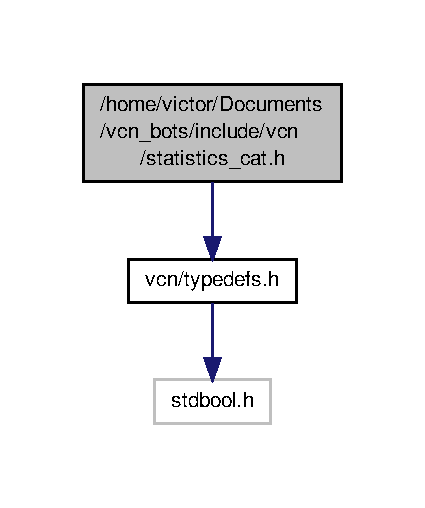
\includegraphics[width=204pt]{statistics__cat_8h__incl}
\end{center}
\end{figure}
\subsection*{Functions}
\begin{DoxyCompactItemize}
\item 
\hypertarget{statistics__cat_8h_aa452fd57961e671b6980a4f45b3c1740}{void {\bfseries runif} (int n, double min, double max, double $\ast$const out, uint $\ast$const seed)}\label{statistics__cat_8h_aa452fd57961e671b6980a4f45b3c1740}

\item 
\hypertarget{statistics__cat_8h_a6bd1afe9bf7ec6eeaf2cef6461dd9f2e}{void {\bfseries rnorm} (int n, double mean, double var, double $\ast$const out, uint $\ast$const seed1, uint $\ast$const seed2)}\label{statistics__cat_8h_a6bd1afe9bf7ec6eeaf2cef6461dd9f2e}

\end{DoxyCompactItemize}


\subsection{Detailed Description}
Simple statistics routines. 

\begin{DoxyAuthor}{Author}
Victor Eduardo Cardoso Nungaray ~\newline
 victorc@cimat.\+mx ~\newline
 \href{https://twitter.com/victore_cardoso}{\tt @victore\+\_\+cardoso } 
\end{DoxyAuthor}
\begin{DoxyDate}{Date}
10 August 2015
\end{DoxyDate}
\begin{DoxyParagraph}{License\+:}
This piece of code is in the P\+U\+B\+L\+I\+C D\+O\+M\+A\+I\+N, if your government does not recognizes such a dedication, then you are granted a perpetual and irrevocable license to copy and modify this file however you want. This does not imply any warranty. ~\newline
 Attributions and feedback are always welcome. 
\end{DoxyParagraph}

\hypertarget{ugrid__dst_8h}{\section{/home/victor/\+Documents/vcn\+\_\+bots/include/vcn/ugrid\+\_\+dst.h File Reference}
\label{ugrid__dst_8h}\index{/home/victor/\+Documents/vcn\+\_\+bots/include/vcn/ugrid\+\_\+dst.\+h@{/home/victor/\+Documents/vcn\+\_\+bots/include/vcn/ugrid\+\_\+dst.\+h}}
}


Uniform Grid Data Structure for geometric fast search.  


{\ttfamily \#include \char`\"{}vcn/typedefs.\+h\char`\"{}}\\*
{\ttfamily \#include \char`\"{}vcn/generic\+\_\+dst.\+h\char`\"{}}\\*
Include dependency graph for ugrid\+\_\+dst.\+h\+:
\nopagebreak
\begin{figure}[H]
\begin{center}
\leavevmode
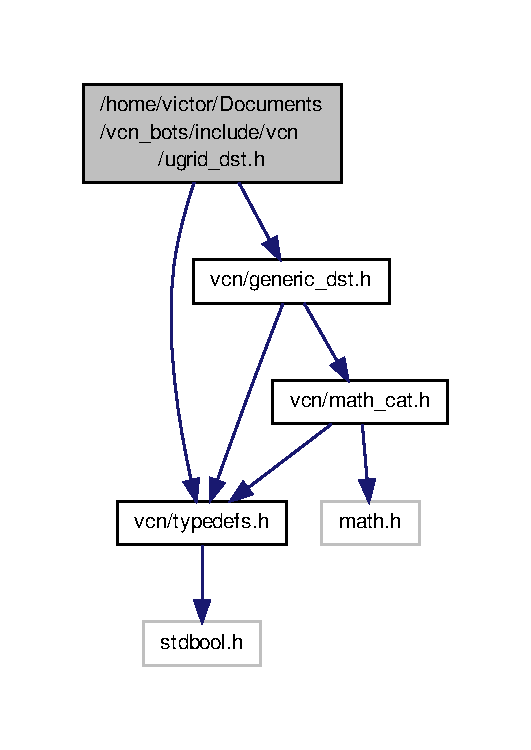
\includegraphics[width=255pt]{ugrid__dst_8h__incl}
\end{center}
\end{figure}
\subsection*{Classes}
\begin{DoxyCompactItemize}
\item 
struct \hyperlink{structpoint__t}{point\+\_\+t}
\end{DoxyCompactItemize}
\subsection*{Typedefs}
\begin{DoxyCompactItemize}
\item 
\hypertarget{ugrid__dst_8h_ac30067c07ae02c1441bb572a3e0425c0}{typedef struct vcn\+\_\+ugrid\+\_\+s {\bfseries vcn\+\_\+ugrid\+\_\+t}}\label{ugrid__dst_8h_ac30067c07ae02c1441bb572a3e0425c0}

\item 
\hypertarget{ugrid__dst_8h_ad493a172b07af0dfa3ecff58e4b0ccf7}{typedef struct vcn\+\_\+ugrid\+\_\+iter\+\_\+s {\bfseries vcn\+\_\+ugrid\+\_\+iter\+\_\+t}}\label{ugrid__dst_8h_ad493a172b07af0dfa3ecff58e4b0ccf7}

\end{DoxyCompactItemize}
\subsection*{Functions}
\begin{DoxyCompactItemize}
\item 
\hypertarget{ugrid__dst_8h_a4567218d5d1e06a700032b7e8369277d}{\hyperlink{structpoint__t}{point\+\_\+t} $\ast$ {\bfseries point\+\_\+create} ()}\label{ugrid__dst_8h_a4567218d5d1e06a700032b7e8369277d}

\item 
\hypertarget{ugrid__dst_8h_a4c693d5ad1fd609adb4f481dcfdd20c4}{void {\bfseries point\+\_\+free\+\_\+attribute\+\_\+and\+\_\+destroy} (\hyperlink{structpoint__t}{point\+\_\+t} $\ast$point)}\label{ugrid__dst_8h_a4c693d5ad1fd609adb4f481dcfdd20c4}

\item 
\hypertarget{ugrid__dst_8h_a500851401886580c65809d8d4c98d196}{void {\bfseries point\+\_\+destroy} (\hyperlink{structpoint__t}{point\+\_\+t} $\ast$point)}\label{ugrid__dst_8h_a500851401886580c65809d8d4c98d196}

\item 
\hypertarget{ugrid__dst_8h_a7e5fb2f816bf71cbd024c768c566ab09}{vcn\+\_\+ugrid\+\_\+t $\ast$ {\bfseries vcn\+\_\+ugrid\+\_\+create} (double size\+\_\+of\+\_\+cells, uint estimated\+\_\+\+N\+\_\+points)}\label{ugrid__dst_8h_a7e5fb2f816bf71cbd024c768c566ab09}

\item 
\hypertarget{ugrid__dst_8h_a930a312e0b990ee85c3f140813336de2}{void {\bfseries vcn\+\_\+ugrid\+\_\+destroy} (vcn\+\_\+ugrid\+\_\+t $\ast$grid, void($\ast$free\+\_\+point)(\hyperlink{structpoint__t}{point\+\_\+t} $\ast$))}\label{ugrid__dst_8h_a930a312e0b990ee85c3f140813336de2}

\item 
\hypertarget{ugrid__dst_8h_a6692f006b685b1b3346dd2a5460e54fe}{void {\bfseries vcn\+\_\+ugrid\+\_\+clear} (vcn\+\_\+ugrid\+\_\+t $\ast$grid, void($\ast$free\+\_\+point)(\hyperlink{structpoint__t}{point\+\_\+t} $\ast$))}\label{ugrid__dst_8h_a6692f006b685b1b3346dd2a5460e54fe}

\item 
\hypertarget{ugrid__dst_8h_aaaf074c7fbd8a1fb36e834345caa39a3}{void {\bfseries vcn\+\_\+ugrid\+\_\+insert} (vcn\+\_\+ugrid\+\_\+t $\ast$const grid, const \hyperlink{structpoint__t}{point\+\_\+t} $\ast$const point)}\label{ugrid__dst_8h_aaaf074c7fbd8a1fb36e834345caa39a3}

\item 
\hypertarget{ugrid__dst_8h_a5ed1b907d4e9fbe48be24ee118bde2f5}{void {\bfseries vcn\+\_\+ugrid\+\_\+remove} (vcn\+\_\+ugrid\+\_\+t $\ast$grid, \hyperlink{structpoint__t}{point\+\_\+t} $\ast$point)}\label{ugrid__dst_8h_a5ed1b907d4e9fbe48be24ee118bde2f5}

\item 
uint \hyperlink{ugrid__dst_8h_a2101c240100566d25ad779bf063b1bf6}{vcn\+\_\+ugrid\+\_\+get\+\_\+knn} (const vcn\+\_\+ugrid\+\_\+t $\ast$const grid, uint k, \hyperlink{structpoint__t}{point\+\_\+t} $\ast$$\ast$knn, double $\ast$knn\+\_\+dist, const \hyperlink{structpoint__t}{point\+\_\+t} $\ast$const p, bool($\ast$filter)(const \hyperlink{structpoint__t}{point\+\_\+t} $\ast$const p\+\_\+ref, const \hyperlink{structpoint__t}{point\+\_\+t} $\ast$const p, const void $\ast$const data), const void $\ast$const filter\+\_\+data)
\begin{DoxyCompactList}\small\item\em Calculate the m nearest neighbours available, with m $<$= k. \end{DoxyCompactList}\item 
\hypertarget{ugrid__dst_8h_a0746e5b5bdd2669d904b643586312941}{vcn\+\_\+list\+\_\+t $\ast$ {\bfseries vcn\+\_\+ugrid\+\_\+get\+\_\+candidate\+\_\+points\+\_\+to\+\_\+min\+\_\+delaunay} (const vcn\+\_\+ugrid\+\_\+t $\ast$const grid, const \hyperlink{structpoint__t}{point\+\_\+t} $\ast$const p1, const \hyperlink{structpoint__t}{point\+\_\+t} $\ast$const p2, bool($\ast$filter)(const \hyperlink{structpoint__t}{point\+\_\+t} $\ast$const p1, const \hyperlink{structpoint__t}{point\+\_\+t} $\ast$const p2, const \hyperlink{structpoint__t}{point\+\_\+t} $\ast$const p, const void $\ast$const data), const void $\ast$const filter\+\_\+data)}\label{ugrid__dst_8h_a0746e5b5bdd2669d904b643586312941}

\item 
\hypertarget{ugrid__dst_8h_a491eabdde896d1286668fe4bbb994e07}{uint {\bfseries vcn\+\_\+ugrid\+\_\+get\+\_\+points\+\_\+inside\+\_\+circle} (const vcn\+\_\+ugrid\+\_\+t $\ast$const grid, double center\mbox{[}2\mbox{]}, double radius, vcn\+\_\+avl\+\_\+t $\ast$output\+\_\+points)}\label{ugrid__dst_8h_a491eabdde896d1286668fe4bbb994e07}

\item 
\hypertarget{ugrid__dst_8h_ab0a1db45ed5cc978a61e93abe51ffe96}{bool {\bfseries vcn\+\_\+ugrid\+\_\+are\+\_\+there\+\_\+points\+\_\+inside\+\_\+circle} (const vcn\+\_\+ugrid\+\_\+t $\ast$const grid, double center\mbox{[}2\mbox{]}, double radius)}\label{ugrid__dst_8h_ab0a1db45ed5cc978a61e93abe51ffe96}

\item 
\hypertarget{ugrid__dst_8h_ae45f8d706083bed77fd3fff57775f5b1}{uint {\bfseries vcn\+\_\+ugrid\+\_\+get\+\_\+ncells} (const vcn\+\_\+ugrid\+\_\+t $\ast$const grid)}\label{ugrid__dst_8h_ae45f8d706083bed77fd3fff57775f5b1}

\item 
\hypertarget{ugrid__dst_8h_a6b9aafc3583d443fcd39d7650ac4818b}{uint {\bfseries vcn\+\_\+ugrid\+\_\+internal\+\_\+vcn\+\_\+htable\+\_\+size} (const vcn\+\_\+ugrid\+\_\+t $\ast$const grid)}\label{ugrid__dst_8h_a6b9aafc3583d443fcd39d7650ac4818b}

\item 
\hypertarget{ugrid__dst_8h_a069a6b80eebd7d72f85197245462b2a3}{uint {\bfseries vcn\+\_\+ugrid\+\_\+min\+\_\+points\+\_\+in\+\_\+a\+\_\+cell} (const vcn\+\_\+ugrid\+\_\+t $\ast$const grid)}\label{ugrid__dst_8h_a069a6b80eebd7d72f85197245462b2a3}

\item 
\hypertarget{ugrid__dst_8h_addab063901af0031ad151957679d005a}{uint {\bfseries vcn\+\_\+ugrid\+\_\+length} (const vcn\+\_\+ugrid\+\_\+t $\ast$const grid)}\label{ugrid__dst_8h_addab063901af0031ad151957679d005a}

\item 
\hypertarget{ugrid__dst_8h_aeb9e1012da46db2ebf3a41162941f05b}{double {\bfseries vcn\+\_\+ugrid\+\_\+get\+\_\+size\+\_\+of\+\_\+cells} (const vcn\+\_\+ugrid\+\_\+t $\ast$const grid)}\label{ugrid__dst_8h_aeb9e1012da46db2ebf3a41162941f05b}

\item 
\hypertarget{ugrid__dst_8h_a49cabc05926799b097ebb6fcf5404de2}{vcn\+\_\+ugrid\+\_\+iter\+\_\+t $\ast$ {\bfseries vcn\+\_\+ugrid\+\_\+iter\+\_\+create} (const vcn\+\_\+ugrid\+\_\+t $\ast$const grid)}\label{ugrid__dst_8h_a49cabc05926799b097ebb6fcf5404de2}

\item 
\hypertarget{ugrid__dst_8h_ae29503fd595c3afe1d889ebe6296acc3}{void {\bfseries vcn\+\_\+ugrid\+\_\+iter\+\_\+destroy} (vcn\+\_\+ugrid\+\_\+iter\+\_\+t $\ast$iter)}\label{ugrid__dst_8h_ae29503fd595c3afe1d889ebe6296acc3}

\item 
\hypertarget{ugrid__dst_8h_a98bebf5e5939e77a0893af8fc51412a4}{\hyperlink{structpoint__t}{point\+\_\+t} $\ast$ {\bfseries vcn\+\_\+ugrid\+\_\+iter\+\_\+get\+\_\+next} (vcn\+\_\+ugrid\+\_\+iter\+\_\+t $\ast$iter)}\label{ugrid__dst_8h_a98bebf5e5939e77a0893af8fc51412a4}

\item 
\hypertarget{ugrid__dst_8h_ab09150af5ca6945a23e194643c42a02e}{char {\bfseries vcn\+\_\+ugrid\+\_\+iter\+\_\+has\+\_\+more} (vcn\+\_\+ugrid\+\_\+iter\+\_\+t $\ast$iter)}\label{ugrid__dst_8h_ab09150af5ca6945a23e194643c42a02e}

\item 
\hypertarget{ugrid__dst_8h_aaea27bb3279cdb5716ca06e4fd74e2d2}{void {\bfseries vcn\+\_\+ugrid\+\_\+iter\+\_\+restart} (vcn\+\_\+ugrid\+\_\+iter\+\_\+t $\ast$iter)}\label{ugrid__dst_8h_aaea27bb3279cdb5716ca06e4fd74e2d2}

\end{DoxyCompactItemize}


\subsection{Detailed Description}
Uniform Grid Data Structure for geometric fast search. 

\begin{DoxyAuthor}{Author}
Victor Eduardo Cardoso Nungaray ~\newline
 victorc@cimat.\+mx ~\newline
 \href{https://twitter.com/victore_cardoso}{\tt @victore\+\_\+cardoso } 
\end{DoxyAuthor}
\begin{DoxyDate}{Date}
10 August 2015
\end{DoxyDate}
\begin{DoxyParagraph}{License\+:}
This piece of code is in the P\+U\+B\+L\+I\+C D\+O\+M\+A\+I\+N, if your government does not recognizes such a dedication, then you are granted a perpetual and irrevocable license to copy and modify this file however you want. This does not imply any warranty. ~\newline
 Attributions and feedback are always welcome. 
\end{DoxyParagraph}


\subsection{Function Documentation}
\hypertarget{ugrid__dst_8h_a2101c240100566d25ad779bf063b1bf6}{\index{ugrid\+\_\+dst.\+h@{ugrid\+\_\+dst.\+h}!vcn\+\_\+ugrid\+\_\+get\+\_\+knn@{vcn\+\_\+ugrid\+\_\+get\+\_\+knn}}
\index{vcn\+\_\+ugrid\+\_\+get\+\_\+knn@{vcn\+\_\+ugrid\+\_\+get\+\_\+knn}!ugrid\+\_\+dst.\+h@{ugrid\+\_\+dst.\+h}}
\subsubsection[{vcn\+\_\+ugrid\+\_\+get\+\_\+knn}]{\setlength{\rightskip}{0pt plus 5cm}uint vcn\+\_\+ugrid\+\_\+get\+\_\+knn (
\begin{DoxyParamCaption}
\item[{const vcn\+\_\+ugrid\+\_\+t $\ast$const}]{grid, }
\item[{uint}]{k, }
\item[{{\bf point\+\_\+t} $\ast$$\ast$}]{knn, }
\item[{double $\ast$}]{knn\+\_\+dist, }
\item[{const {\bf point\+\_\+t} $\ast$const}]{p, }
\item[{bool($\ast$)(const {\bf point\+\_\+t} $\ast$const p\+\_\+ref, const {\bf point\+\_\+t} $\ast$const p, const void $\ast$const data)}]{filter, }
\item[{const void $\ast$const}]{filter\+\_\+data}
\end{DoxyParamCaption}
)}}\label{ugrid__dst_8h_a2101c240100566d25ad779bf063b1bf6}


Calculate the m nearest neighbours available, with m $<$= k. 

\begin{DoxyReturn}{Returns}
The output is sorted based on the dist(...) function. 
\end{DoxyReturn}

%--- End generated contents ---

% Index
\newpage
\phantomsection
\addcontentsline{toc}{chapter}{Index}
\printindex

\end{document}
